%Thesis Main Page used with thesis.sty (Dorothea Brosius, August 2006) based on the
%University of Maryland, College Park  "Thesis and Dissertation Style Guide," 
%2005-2006, Fall 2005 Edition

\documentclass[12pt]{thesis-2}  % USE 12 IN FINAL VERSION
%\documentclass[11pt]{nice-thesis}
\usepackage{times}
\usepackage[svgnames]{xcolor}
\usepackage[sort,round]{natbib}
\usepackage{lscape}
\usepackage{indentfirst}
\usepackage{latexsym}
\usepackage{multirow}
\usepackage{amsmath}
\usepackage[pointedenum]{paralist}
\usepackage{amssymb}
\usepackage{amsthm}
\usepackage[noend]{algpseudocode}
% Chinese stuff (borrowed from HLT 2005 paper)
\usepackage{CJK}
\usepackage{ucs}
\usepackage[utf8x]{inputenc}
\usepackage{mathptm}
\usepackage{afterpage}
\usepackage{tikz}
\usepackage{sparklines}
\usepackage{hyperref}
\usepackage{lopez}
\usepackage{extraction-fig-macros}

\hypersetup{
    pdftitle={Machine Translation by Pattern Matching},    % title
    pdfauthor={Adam Lopez},     % author
    pdfsubject={computer science},   % subject of the document
    colorlinks=true,       % false: boxed links; true: colored links
    linkcolor=MidnightBlue,          % color of internal links
    citecolor=MidnightBlue,        % color of links to bibliography
    urlcolor=DarkGreen           % color of external links
}



\usetikzlibrary{snakes}
\usetikzlibrary{matrix}

\pdfmapfile{+cyberbit}
\newcommand{\zh}[1]{\begin{CJK*}{UTF8}{cyberbit}#1\end{CJK*}}


\renewcommand{\baselinestretch}{2} % 2 IN OFFICIAL VERSION
\setlength{\textwidth}{5.9in}
\setlength{\textheight}{9in}
\setlength{\topmargin}{-.50in}
\setlength{\oddsidemargin}{.55in}
\setlength{\parindent}{.4in}
\pagestyle{empty}

\newcommand{\figpreamble}{\renewcommand{\baselinestretch}{1}}
\newcommand{\figpostamble}{\renewcommand{\baselinestretch}{2}} % 2 IN OFFICIAL VERSION
\newcommand{\figfontsize}[1]{{\small #1}} % USE IN OFFICIAL VERSION
%\newcommand{\figfontsize}[1]{#1} 

\begin{document}

%Abstract Page 

\hbox{\ }

\figpreamble
% \renewcommand{\baselinestretch}{1} % USE IN FINAL VERSION
\small \normalsize

{\LARGE \begin{center}Abstract\end{center}} % this is a bit hackish
%\addcontentsline{toc}{chapter}{Abstract}
%\vspace{20pt}

\vspace{3em} 

\hspace{-.15in}
\begin{tabular}{ll}
Title of dissertation:    & {\sc Machine Translation by Pattern Matching}\\
& \\
&                          {Adam Lopez, Doctor of Philosophy, 2008}\\ 
& \\
Dissertation directed by: & {Professor Philip Resnik} \\
&  				{Department of Linguistics and} \\
&  				{Institute for Advanced Computer Studies} \\
\end{tabular}
\figpostamble

\vspace{3em}

%\renewcommand{\baselinestretch}{2}
\large \normalsize
The best systems for machine translation of natural language
are based on statistical models learned from data.  Conventional
representation of a statistical translation model requires substantial
offline computation and representation in main memory.
Therefore, the principal bottlenecks to the amount of data we can exploit
and the complexity of models we can use are available memory and CPU time,
and current state of the art already pushes these limits.  With data size
and model complexity continually increasing, a scalable solution to this
problem is central to future improvement.

\citet{Callison-Burch:2005:acl} and \citet{Zhang:2005:eamt} proposed a solution
that we call {\em translation by pattern matching}, which we bring to fruition
in this dissertation.  The training data itself serves as a proxy to the
model; rules and parameters are computed on demand.  It achieves our
desiderata of minimal offline computation and compact representation, but is
dependent on fast pattern matching algorithms on text.  They demonstrated
its application to a common model based on the translation of contiguous
substrings, but leave some open problems.  Among these is a question: can
this approach match the performance of conventional methods despite
unavoidable differences that it induces in the model?  We show how to answer
this question affirmatively.

The main open problem we address is much harder.  Many translation models
are based on the translation of discontiguous substrings.  The best pattern
matching algorithm for these models is much too slow, taking several minutes
per sentence.  We develop new algorithms that reduce empirical computation
time by two orders of magnitude for these models, making translation by
pattern matching widely applicable.  We use these algorithms to build a
model that is two orders of magnitude larger than the current state of the
art and substantially outperforms a strong competitor in Chinese-English
translation.  We show that a conventional representation of this model would
be impractical.  Our experiments shed light on some interesting properties
of the underlying model.  The dissertation also includes the most
comprehensive contemporary survey of statistical machine translation.


 %(must be first, required, non-numbered) 
\renewcommand{\baselinestretch}{1}
%Titlepage

\thispagestyle{empty}
\hbox{\ }
\vspace{1in}
\small\normalsize
\begin{center}

\huge{{\sc Machine Translation by Pattern Matching}}\\
\ \\
\large{by} \\
\ \\
\large{Adam David Lopez}%Your full name as it appears in University records.
\ \\
\ \\
\ \\
\ \\
\normalsize
Dissertation submitted to the Faculty of the Graduate School of the \\
University of Maryland, College Park in partial fulfillment \\
of the requirements for the degree of \\
Doctor of Philosophy \\
2008
\end{center}

\vspace{7.5em}

\noindent Advisory Committee: \\
Professor Philip Resnik, Chair/Advisor \\
Professor David Chiang \\
Professor Bonnie Dorr \\
Professor David Fushman \\
Professor Douglas Oard
 %(must follow Abstract, required, non-numbered)
\renewcommand{\baselinestretch}{2} % 2 IN OFFICIAL VERSION
%Copyright

\thispagestyle{empty}
\hbox{\ }

\vfill
% \renewcommand{\baselinestretch}{1} % USE IN FINAL VERSION
\small\normalsize

\vspace{-.65in}

%\chapter*{} % this is a bit hackish
%\addcontentsline{toc}{chapter}{Copyright}

\begin{center}
\large{\copyright{} Adam Lopez 2008\\
~\\
Licensed under the \textit{Creative Commons Attribution-Noncommercial-Share Alike 3.0} license %
(http://creativecommons.org/licenses/by-nc-sa/3.0/). %
Some rights reserved.\\
~\\
A portion of this work is based on: Statistical Machine Translation, in {\em ACM Computing Surveys}, 40(3), Aug. \copyright{} Association for Computing Machinery, 2008.  \url{http://doi.acm.org/10.1145/1380584.1380586}}
\end{center}

\vfill
 %(highly recommended, non-numbered)

%Pages from this point start at lower-case Roman number ii)
\pagestyle{plain}
\pagenumbering{roman}
\setcounter{page}{2}

%\include{Preface}  %(if present, start at lower-case Roman number ii)
%\include{Foreword} %(if present, lower-case Roman)
%Dedication

% \renewcommand{\baselinestretch}{2} % USE IN FINAL VERSION
\small\normalsize
\hbox{\ }
 
\vspace{-.65in}

\chapter*{} % this is a bit hackish
\addcontentsline{toc}{chapter}{Dedication}

\vspace{2cm}

\begin{center}
For Jennifer.
\end{center} 

 %(if present, lower-case Roman)
%Acknowledgments

\small\normalsize
\hbox{\ }
 
\vspace{-.65in}


\chapter*{\LARGE \begin{center}Acknowledgements\end{center}} % this is a bit hackish
\addcontentsline{toc}{chapter}{Acknowledgements}
\vspace{40pt}


I am deeply indebted to Philip Resnik for guiding me through this process.  This dissertation is a testament to his faith in me, which was often greater than my own.  I would not have found my own path if he had not given me the freedom to get lost, and direction when I stayed lost for too long.  His enthusiasm and encouragement were crucial to my success, and I can only hope that I one day inspire someone else as much as he has inspired me.

I am also grateful for the guidance of my committee---David Chiang, Bonnie Dorr, Doug Oard, and David Fushman.  
Much of the work described herein was influenced in one way or another by my interactions with David Chiang.  In 2005, I asked him whether the suffix array trick would work with hierarchical models, and he told me he didn't think so.  It's about the only time I've ever known him to be wrong about anything, and even that took over two years and an enormous amount of work to prove.  David also gave me very constructive early feedback that shaped the survey chapter, and it is not hyperbole to say that I learned much of what I know about statistical translation just from reading his elegant code.
Bonnie Dorr gave me tremendously detailed and helpful feedback on several drafts of the dissertation, and Doug Oard directly challenged me to broaden its scope and vision.  The final result is much stronger than it would have been without them.
Finally, David Fushman gamely served on my committee and engaged with me throughout this process even though his own work is very far afield from mine.  Together with Philip, they held this dissertation to a high standard.  Any errors that remain are my own.

Several people in the Department of Computer Science and UMIACS helped along the way.  I am grateful to Bill Gasarch for serving on my proposal committee, but more importantly for his unvarnished advice.  Mihai Pop graciously allowed me to audit and actively engage with his bioinformatics seminar, where I found most of the tools that I needed to solve David's challenge.  Fritz McCall went above and beyond the call of the duty assisting me through my forays into network programming.

I learned most of what I know about natural language processing from the present and past students, postdoctoral researchers, and visitors who have been my colleagues in the CLIP lab.  Many ideas were developed and refined in discussions with
Fazil Ayan,
Dina Demner-Fushman,
Mona Diab,
Nizar Habash,
Tim Hunter,
Okan Kolak,
Nitin Madnani,
Smaranda Muresan,
Christof Monz,
Mike Nossal,
Michael Subotin,
Davic Zajic, and
Dan Zeman.
I owe special thanks to Chris Dyer for all of the brainstorming, critiquing, and commiserating during the course of writing this dissertation.  Most especially, I thank Rebecca Hwa for being my mentor and my friend.

Outside of the lab, I thank Bill Woods for my earliest exposure to NLP research, and I'm enormously grateful to Philipp Koehn---first for offering me a fantastic job that I'm very excited about, and then for waiting on me while I completed this obligation.

I had a lot of fun in grad school.  This I owe to the friends I spent time with outside of the lab:
Laura Bright,
Gene Chipman,
Ric Crabbe,
Shaun Gittens,
Debbie Heisler,
Omer Horvitz,
Dave Hovemeyer,
Doc Hunter,
Aram Khalili,
Jordan Landes,
Jeremy Manson,
Jan Neumann,
Brian Postow,
Reiner Schulz,
Jaime Spacco,
Kate Swope, and
Chadd Williams.
Thank you all for keeping me sane.

My family has been supportive of me throughout this endeavor, even though it seemed prolonged and bewildering when beheld from afar.  I am thankful to Lisa and Josh Friedman, and my parents Richard and Edith Lopez.

Most importantly, Jennifer Baugher has filled my days, nights, and dreams with love throughout my time here.  She has been with me for every moment of triumph and despair, through countless adventures and many bottles of wine.  I know I could accomplish anything when she is with me.  Thank you for everything, for ever.

\newpage
~
\vspace{1.5in}

This research was supported in part by NSA Contract RD-02-5700, ONR MURI Contract FCPO.810548265 and the GALE program of the Defense Advanced Research Projects Agency, Contract No. HR0011-06-2-001. 
Any opinions, findings, conclusions or recommendations expressed in this work are those of the author and do not necessarily reflect the view of DARPA.  
Additional support was provided by the EuroMatrix project funded by the European Commission (6th Framework Programme).


 %(if present, lower-case Roman)

\renewcommand{\baselinestretch}{1}
\small\normalsize
\chapter*{} %hack
\addcontentsline{toc}{chapter}{Contents}
\tableofcontents %(required, lower-case Roman)
\newpage
\setlength{\parskip}{1em}
\listoftables %(if present, lower-case Roman)
\newpage
\listoffigures %(if present, lower-case Roman) % USE IN FINAL VERSION
\newpage % USE IN FINAL VERSION

\newpage
\setlength{\parskip}{0em}
\renewcommand{\baselinestretch}{2} % 2 IN OFFICIAL VERSION
\small\normalsize

%Pages from this point start at Arabic numeral 1
\setcounter{page}{1}
\pagenumbering{arabic}

\renewcommand{\topfraction}{1}

\chapter{Introduction}\label{chap:introduction}

\begin{quote}
	{\em Computer Science is no more about computers than astronomy is about telescopes.}
	\begin{flushright}
		--Edsger Dijkstra
	\end{flushright}
\end{quote}
\begin{quote}
	{\em The purpose of computing is insight, not numbers.}
	\begin{flushright}
		--Richard Hamming
	\end{flushright}
\end{quote}

Machine translation is an old problem.  Like many other
computational problems it has been largely reinvented in 
the last fifteen years through the incorporation of machine 
learning methods.  The machine learning approach to machine
translation---called {\em statistical machine translation}---
requires considerable data and careful modeling.  
With available data increasing in size
and the best models increasing in complexity,
efficient algorithms are central to continued
progress.  This dissertation presents an algorithmic approach
to statistical machine translation that enables scaling to
large data and complex models, and fosters the rapid experimentation
needed to exploit them.

Most statistical machine translation systems implement a 
{\em direct representation} of the model.  This entails
offline computation of the complete model and storage of
this model in an efficient data structure in main memory 
at runtime.  In practice, these requirements
restrict the size of training data and the complexity
of the model, since both factors can affect model size.

\citet{Callison-Burch:2005:acl} and \citet{Zhang:2005:eamt}
proposed an alternative that we call {\em translation by pattern matching},
which we bring to fruition in this dissertation.  This
approach relies on an indirect representation of the model.
We store the training data itself in memory as its proxy.
Model parameters are then computed as needed at runtime.  This
representation is much more compact than the full model
and requires substantially less offline computation.  
It depends crucially on the ability to quickly search for 
relevant sections of the training data and compute
parameters as needed.   To perform this search, we need
algorithms for fast pattern matching on text, drawn primarily
from the literature in bioinformatics and information
retrieval.  Although
\citet{Callison-Burch:2005:acl} and \citet{Zhang:2005:eamt}
resolve several problems in the application of translation
by pattern matching to a standard phrase-based model, they leave behind several
open problems.  The first is whether their approach
can equal the performance of direct representation, 
a question that we answer affirmatively.

The next open problem we address is much harder.
\citet{Callison-Burch:2005:acl} and \citet{Zhang:2005:eamt}
applied their approach only to phrase-based translation models 
based on the translation of contiguous strings.  However,
a variety of translation models are now based on the 
translation of {\em discontiguous} phrases.  This new wrinkle
poses a difficult algorithmic challenge.
Exact pattern matching algorithms used for contiguous phrases don't work and
the best approximate pattern matching algorithms are much too slow,
taking several minutes per sentence.  A major contribution of
this dissertation is the development of new approximate 
pattern matching algorithms for translation models based on
discontiguous phrases.  Our algorithms reduce the empirical computation
time by two orders of magnitude, making translation by pattern matching
feasible for these models.

With these tools in hand, we address the problem of scaling
our translation model.  We then explore several scaling axes---some obvious and 
some novel---and show that we can significantly improve on 
a state-of-the-art hierarchical phrase-based translation system.  
Our experiments highlight interesting characteristics of the model
and interactions of various components.
Finally, we conclusively demonstrate that reproducing our results
with a direct representation would be extremely impractical.

\section{Outline of the Dissertation}

To set the stage for our research, Chapter~\ref{chap:survey} surveys the
current state of the art in statistical machine translation.  This is the
most extensive contemporary survey of the field.  It serves as a foundation 
on which the remaining chapters build.

Chapter~\ref{chap:overview} introduces translation by pattern matching.  We first
review previous work that serves as inspiration for our approach.  We then identify
some limitations of this work
and describe how we overcame these, transforming a clever idea into a 
practical solution.  We establish for the first time 
that translation by pattern matching is a
viable replacement for direct representation in a state-of-the-art phrase-based
translation model.

In Chapter~\ref{chap:algorithms} we apply translation by pattern matching to models
based on the translation of discontiguous strings.  This requires the invention 
of new pattern matching algorithms.  We describe our
algorithms in detail and analyze them theoretically and empirically.  Our algorithms
allow us to apply translation by pattern matching to hierarchical
phrase-based translation, a stronger baseline than the model used
in \ref{chap:overview}.  It matches the state of the art
achieved by direct representation.

In Chapter~\ref{chap:scaling} we apply translation by pattern matching to the problem of scaling
translation models.  We describe a number of axes along which
we can scale the models and investigate each of these empirically.  We then show
that our scaling methods improve translation quality over our strong
baseline.  Our experiments illuminate some interesting qualities
of these models and their interaction with aligned bilingual texts.  Finally,
we demonstrate that our results would be extremely difficult to replicate
using a direct representation.

Chapter~\ref{chap:conclusion} contains conclusions and future work.  We also
relate our work to other developments in the field, and describe
future research plans.

\section{Research Contributions}

The dissertation contains several important research contributions.

\begin{itemize}

	\item We describe a complete algorithmic framework for machine translation
	by pattern matching that enables scaling to large data, richer modeling,
	and rapid prototyping.

	\item We identify unanswered questions in the prior work that provides the foundation
	of our framework, and describe how we answer them to give
	state-of-the-art performance in standard phrase-based translation models.

	\item We introduce a novel approximate pattern matching algorithm that
	extends our framework to a variety of important models based on 
	discontiguous phrases.  Our algorithm solves an empirically difficult algorithmic problem.  
	It is two orders of magnitude faster than the previous state of the art, and 
	enables a number of previously difficult or impossible applications.

	\item We show how our framework can be applied to scale statistical translation
	models along several axes, leading to improvement in translation accuracy over
	a state-of-the-art baseline.

	\item We show that our method can scale to extremely large models, at least
	two orders of magnitude larger than most contemporary models.

	\item We include the most comprehensive survey of the field of statistical
	machine translation to date.
\end{itemize}








\chapter{A Survey of Statistical Machine Translation}\label{chap:survey}

\begin{quote}
	{\em It is very tempting to say that a book written in Chinese is simply a 
	book written in English which was coded into the “Chinese code.” If we 
	have useful methods for solving almost any cryptographic problem, may it 
	not be that with proper interpretation we already have useful methods for 
	translation?}
	\begin{flushright}
		--Warren Weaver
	\end{flushright}
\end{quote}


We begin with a tutorial overview and survey of 
statistical machine translation.\footnote{This chapter has been accepted to appear in {\em ACM Computing Surveys} \citep{Lopez:2008:csur}.}  It is the most
comprehensive contemporary survey of this rapidly growing field.
Additionally, it introduces many of the concepts and definitions
that are used throughout the remainder of the dissertation.  The 
organization is horizontal---we show that the creation of a statistical
translation system requires making a number of important decisions, but 
that many of these decisions are in fact orthogonal.  Two
systems that are radically different in one aspect may nonetheless share
a common basis in several other aspects.  We believe that this type of
organization is beneficial to continued progress of the field since
it encourages cross-pollination of ideas.

The goals of this chapter are to characterize 
the core ideas of SMT and provide a taxonomy of  
various approaches.  We have tried to make the
survey as self-contained as possible.  
However, SMT draws from many
fundamental research areas in computer science, so some
knowledge of automata theory, formal languages, 
search, and data structures will be beneficial.
Familiarity with statistical theory
and mathematical optimization techniques used in 
machine learning will also be helpful,
but we will focus on the main ideas and intuitions 
behind the mathematics rather than 
full mathematical rigor, which
is in any case beyond the scope of this work.
We will touch briefly on a few linguistic concepts, 
but for our purposes SMT can be understood in
pure computer science terms.

\section{Previous Work}

\citet{Knight:1997:ai,Knight:1999:unpublished} has 
written excellent tutorial introductions, but they do not 
cover many later developments in the field.
\citet{Knight:2005:icassp} briefly survey the recent landscape, while 
\citet[chapter 2]{Ayan:2005:thesis} provides a longer treatment, focusing
primarily on word alignment (\textsection\ref{sec:word-alignment}).
At the time of this writing, other materials 
in preparation include \citet{Koehn:2008:book} 
and a chapter in a planned future
edition of \citet{Jurafsky:2000:book}.  For greater 
coverage of related fundamental research, 
refer to textbooks on natural language processing
\citep[NLP;][]{Manning:1999:book,Jurafsky:2000:book},
artificial intelligence \citep{Russell:2003:book}
machine learning \citep{Mitchell:1997:book},
or formal language theory \citep{Hopcroft:1979:book,Sipser:2005:book}.


\section{Background and Context}\label{sec:background-and-context}

\term{Machine translation} (MT) is the
automatic translation from one natural
language into another using computers.  Interest in 
MT is nearly as old as the electronic
computer---popular accounts trace
its modern origins to a letter written by Warren Weaver
in 1949, only a few years after ENIAC came online.\footnote{
This letter is reproduced as \citet{Weaver:1955:mt}.}
It has since remained
a key application in the field of natural
language processing (NLP).
A good historical overview is given by 
\citet{hutchins:2006:cuhk}, and a comprehensive
general survey is given by \citet{Dorr:1999:aic}.

\term{Statistical machine translation} (SMT) 
is an approach to MT
that is characterized by the use of machine
learning methods.  In less than two decades,
SMT has come to dominate academic MT research,
and has gained a share of the commercial MT market.
Progress is rapid and the state-of-the-art 
is a moving target.  However, as the field has matured, 
some common themes have emerged.

SMT treats translation as a machine learning problem.  
This means that we apply a learning algorithm to a large body of 
previously translated text, known variously as
a \term{parallel corpus}, \term{parallel text}, 
\term{bitext}, or \term{multitext}.
The learner is then able translate
previously unseen sentences.  With an SMT toolkit and 
enough enough parallel text, we can build an MT system for
an new language pair within a very short period of time---
perhaps as little as a day 
\citep{Al-Onaizan:1999:tr,Oard:2003:mtsummit,Oard:2003:naacl}.
For example, \citet{Oard:2003:mtsummit} report
constructing a Cebuano-to-English SMT system in a matter of 
weeks.  Workshops have shown that translation systems
can be built for a wide variety of language pairs within
similar time frames \citep{Koehn:2005:wpt,Koehn:2006:smt,Callison-Burch:2007:smt}.
The accuracy of these systems depends crucially on the quantity,
quality, and domain of the data,
but there are many tasks for which even poor translation 
is useful \citep{Church:1993:mt}.  

Interest in SMT can be attributed to the convergence of
several factors.

\begin{asparaenum}
\item The growth of the Internet has strongly affected
two constituencies of translation consumers.  The first 
of these is interested in the \term{dissemination}
of information in multiple languages.  Examples are multilingual
governments and news agencies and companies
operating in the global marketplace.  The Internet enables them
to easily publish information in multiple languages.
Due to this widespread dissemination, SMT researchers 
now have access to Biblical texts \citep{Resnik:1997:tei}, 
bilingual government text \citep{Koehn:2005:mtsummit}, 
bilingual news text, and
other data mined from the Internet \citep{Resnik:2003:cl}.
These data are the fundamental resource in SMT research. 
Because they are the product of day-to-day human activities,
they are constantly growing.  Multilingual governments 
interested in dissemination, such as the European Union,
have increased MT research funding to further
their domestic policy interests.

\item The other consumers of translation are those
interested in the \term{assimilation} of information not in their
native language.  These include intelligence agencies, researchers,
and casual Internet users.  The Internet has made such information
much more readily accessible, and
increasing demand from these users helps drive popular interest in MT.
The United States government is interested in
assimilation, and has increased MT research funding
to further its international policy interests.

\item Fast, cheap computing hardware has enabled applications
that depend on large data and billions of statistics.
Advances in processor speed, random access memory 
size, secondary storage, and
grid computing have all helped to enable SMT.

\item The development of automatic translation 
metrics---although controversial---has
enabled rapid iterative development of MT systems and 
fostered competition between research groups.  Objective
measurable goals have naturally led to objective
measurable progress.  The National Institute of Standards
has used these metrics since 2002 in a yearly competition at its
MT Evaluation conference.\footnote{These evaluations
are described at \url{http://www.nist.gov/speech/tests/mt}.}
Academic workshops coordinate similar evaluations
\citep{Koehn:2005:wpt,Koehn:2006:smt,Callison-Burch:2007:smt}.

\item Several projects have focused on the development
of freely available SMT toolkits
\citep{Al-Onaizan:1999:tr,Germann:2001:acl,Och:2003:cl,Koehn:2004:amta,Burbank:2005:tr,Olteanu:2006:smt,Koehn:2007:acl-demo}.
Many are open-source.  These implementations help lower the barrier for entry
into SMT research.
\end{asparaenum}

\subsection{Formal Description} \label{sec:formal-description}

Formally, our task is to take a sequence of tokens in
the \term{source language} with vocabulary $V_F$, 
and transform it into a sequence of tokens in the 
\term{target language} with vocabulary 
$V_E$.\footnote{We follow the widely used notation
of \citet{Brown:1993:cl}, who use $E$ for English and 
$F$ for French (or foreign).}  We will assume that 
tokens are words and sequences are sentences. 
Agglutinative languages
such as German and Inuktitut, or languages with no clearly marked
word boundaries, such as Chinese, may require special preprocessing. 
The most important consideration is that all data are
preprocessed consistently, since statistical systems are sensitive
to discrepancies.  There is often no special
treatment of morphological variants---for instance, the English 
words {\em translate} and {\em translation} are treated as unrelated,
indivisible tokens.  Therefore, it is possible for the size
of the vocabularies $V_E$ and $V_F$ to reach into the tens or
hundreds of thousands, or even millions in the case of 
morphologically complex languages such as Arabic.

We denote a sequence of $J$ source words 
as $f_1 f_2... f_J$ or $f_1^J \in {V_F}^J$, 
and a sequence of $I$ target words as 
$e_1 e_2... e_I$ or $e_1^I \in {V_E}^I$.
The goal of a translation system, when 
presented with an input sequence $f_1^J$,
is to find a sequence $e_1^I$ that is
\term{translationally equivalent}. 

An example of translationally equivalent sequences is 
shown in \figureref{example}.  An exercise
familiar to those who have learned a foreign
language is to draw a line between the words in the sentence
that are translations of each other.  For instance,
we can see that Chinese word \zh{北} is translated as
the English word {\em north}, and we could draw 
a line between them.  We say that such 
words are \term{aligned}.  An example word alignment is shown in 
\figureref{alignment}.  This illustrates 
that translational equivalence can be decomposed into
a number of smaller equivalence problems at the word level.

\figpreamble
\begin{figure*}[t]
\figfontsize{\begin{center}
\begin{tikzpicture}[node distance=1cm]

	% this figure uses invisible nodes to make the
	% top and bottom of the alignment links to line up,
	% which is a little hacky.
	\matrix (english sentence) [nodes={anchor=mid}] {
		\node {However}; & 
		\node{,}; & 
		\node{the}; & 
		\node{sky}; & 
		\node{remained}; & 
		\node{clear}; & 
		\node{under}; & 
		\node{the}; & 
		\node{strong}; & 
		\node{north}; & 
		\node{wind}; & 
		\node{.}; \\
		\node (english however){}; & 
		\node (english comma){}; & 
		\node (english the){}; & 
		\node (english sky){}; & 
		\node (english remained){}; & 
		\node (english clear){}; & 
		\node (english under){}; & 
		\node (english the){}; & 
		\node (english strong){}; & 
		\node (english north){}; & 
		\node (english wind){}; & 
		\node (english period){};\\
	};

	\matrix (chinese sentence) [nodes={anchor=mid},column sep=1.5,below of=english sentence] {
		\node (chinese although){}; & 
		\node (chinese north){}; & 
		\node (chinese wind){}; & 
		\node (chinese howls){}; & 
		\node (chinese comma){}; & 
		\node (chinese but){}; & 
		\node (chinese sky){}; & 
		\node (chinese still){}; & 
		\node (chinese extremely){}; & 
		\node (chinese limpid){}; & 
		\node (chinese period){}; \\
		\node{\zh{虽然}}; & 
		\node{\zh{北}}; & 
		\node{\zh{风}}; & 
		\node{\zh{呼啸}}; & 
		\node{\zh{,}}; & 
		\node{\zh{但}}; & 
		\node{\zh{天空}}; & 
		\node{\zh{依然}}; & 
		\node{\zh{十分}}; & 
		\node{\zh{清澈}}; & 
		\node{~~\zh{。}}; \\
		\node{\em Although}; & 
		\node{\em north}; & 
		\node{\em wind}; & 
		\node{\em howls}; & 
		\node{\em ,}; & 
		\node{\em but}; & 
		\node{\em sky}; & 
		\node{\em still}; & 
		\node{\em extremely}; & 
		\node{\em limpid}; & 
		\node{\em .~}; \\
	};

\end{tikzpicture}

\end{center}}
\figpostamble
\caption[An example of translationally equivalent sentences.]{\label{fig:example}An example of translationally equivalent sentences.  We give an English gloss for each Chinese word.}
\end{figure*}

Word translation is often ambiguous.  
For instance, we might reasonably translate \zh{北} 
 as {\em northern} without loss of
meaning.  However, it is not uncommon for the different
possible translations of a word to have very different
meanings.  Often, the correct choice
will depend on context.  Therefore, our 
system will need some mechanism to choose between 
several possible options for each translation decision.

In addition to word translation, the other main
problem that can be seen from the figure is that
words with equivalent meanings do not appear in the
same order in both sentences.  Therefore, our
system will need some mechanism to correctly {\em reorder} the
words.  Reordering is typically dependent on the syntactic
structure of the target language.  For instance, in English
sentences, the typical sentence order is 
{\em subject-verb-object} (SVO).  In
Japanese, it is {\em subject-object-verb} (SOV).
As with word translation, reordering decisions often
entail resolving some kind of ambiguity.

Translation can therefore be thought of as making
a sequence of word translation and reordering
decisions.  We rewrite the source sentence
one decision at a time, until we have replaced
it completely with a target sentence.  At each decision
point, a large number of possible rules may apply.  We
will need some mechanism to disambiguate these rules.
Furthermore, both rules and methods of disambiguation
must be learned from our parallel data.

Following these core ideas, there are 
four problems that we must solve in order
to build a functioning SMT system.

\begin{asparaenum}

\item First, we must describe the series of steps
that transform a source sentence into a target sentence.
We can think of this as creating a story about how a human
translator might perform this task.  This story is called
a {\em translational equivalence model}, or more simply a
{\em model}.  All of the translational equivalence models
that we will consider derive from concepts from
automata and language theory.  We describe them in 
\sectionref{translational-equivalence-models}.

\item Next, we want to enable our model to make good
choices when faced with a decision to resolve some ambiguity.
We need to develop a {\em parameterization} of the model that will
enable us to assign a score to every possible source and target
sentence pair that our model might consider. We describe 
parameterization in \sectionref{mathematical-modeling}.
Taken together, translational equivalence modeling and
parameterization are often combined under the rubric of
{\em modeling}.\footnote{Although these two steps
are conflated under this term in the literature, 
following \citet{Brown:1990:cl}, for didactic 
reasons we find it helpful to separate them.}

\item The parameterization defines a set of statistics 
called {\em parameters} used to score the model,
but we need to associate values to these parameters.
This is called \term{parameter estimation}, and it
is based on machine learning methods.
We describe parameter estimation 
in \sectionref{parameter-estimation}.

\item Finally, when we are presented with 
input sentence, we must search for the
highest-scoring translation according to our model.  
This is called \term{decoding}.  
We describe decoding in 
\sectionref{decoding}.
\end{asparaenum} 

\figpreamble
\begin{figure*}[t]
\figfontsize{\begin{center}
\begin{tikzpicture}[node distance=2cm]

	% this figure uses invisible nodes to make the
	% top and bottom of the alignment links to line up,
	% which is a little hacky.
	\matrix (english sentence) [nodes={anchor=mid}] {
		\node {However}; & 
		\node{,}; & 
		\node{the}; & 
		\node{sky}; & 
		\node{remained}; & 
		\node{clear}; & 
		\node{under}; & 
		\node{the}; & 
		\node{strong}; & 
		\node{north}; & 
		\node{wind}; & 
		\node{.}; \\
		\node (english however){}; & 
		\node (english comma){}; & 
		\node (english the){}; & 
		\node (english sky){}; & 
		\node (english remained){}; & 
		\node (english clear){}; & 
		\node (english under){}; & 
		\node (english the){}; & 
		\node (english strong){}; & 
		\node (english north){}; & 
		\node (english wind){}; & 
		\node (english period){};\\
	};

	\matrix (chinese sentence) [nodes={anchor=mid},column sep=1.5,below of=english sentence] {
		\node (chinese although){}; & 
		\node (chinese north){}; & 
		\node (chinese wind){}; & 
		\node (chinese howls){}; & 
		\node (chinese comma){}; & 
		\node (chinese but){}; & 
		\node (chinese sky){}; & 
		\node (chinese still){}; & 
		\node (chinese extremely){}; & 
		\node (chinese limpid){}; & 
		\node (chinese period){}; \\
		\node{\zh{虽然}}; & 
		\node{\zh{北}}; & 
		\node{\zh{风}}; & 
		\node{\zh{呼啸}}; & 
		\node{\zh{,}}; & 
		\node{\zh{但}}; & 
		\node{\zh{天空}}; & 
		\node{\zh{依然}}; & 
		\node{\zh{十分}}; & 
		\node{\zh{清澈}}; & 
		\node{~~\zh{。}}; \\
		\node{\em Although}; & 
		\node{\em north}; & 
		\node{\em wind}; & 
		\node{\em howls}; & 
		\node{\em ,}; & 
		\node{\em but}; & 
		\node{\em sky}; & 
		\node{\em still}; & 
		\node{\em extremely}; & 
		\node{\em limpid}; & 
		\node{\em .~}; \\
	};

	\draw (english however.north) -- (english however.north |- chinese  although.south);
	\draw (english however.north)  -- (chinese  but.south);
	\draw (english comma.north)  -- (chinese  comma.south);
	\draw (english sky.north)  -- (chinese  sky.south);
	\draw (english remained.north)  -- (chinese  still.south);
	\draw (english clear.north)  -- (chinese  limpid.south);
	\draw (english strong.north)  -- (chinese  howls.south);
	\draw (english north.north)  -- (chinese  north.south);
	\draw (english wind.north)  -- (chinese  wind.south);
	\draw (english period.north) -- (english period.north |- chinese  period.south);
\end{tikzpicture}

\end{center}}
\figpostamble
\caption{\label{fig:alignment}An alignment of
the the sentence in \figureref{example}.}
\end{figure*}

In addition to these four problems, we will 
discuss the important 
topic of evaluation in \sectionref{evaluation}.  The 
article concludes with notes on current directions 
in \sectionref{future-research}.

\section{Modeling Part I: Translational Equivalence}\label{sec:translational-equivalence-models}

Broadly speaking, 
a  model is simply the set of
all rules employed by an MT system to transform a source
sentence into a target sentence.  In principle
these rules may come from anywhere.  In most SMT systems
they are automatically extracted from a 
parallel corpus.  The extraction process is described in
more detail in \sectionref{word-alignment}.  In this 
section, we describe the various types of models.

Most popular models
can be described by one of two formalisms:
finite-state transducers (FST) or 
synchronous context-free grammars (SCFG).\footnote{
This distinction may be confusing, since finite
state transducers come to us from automata theory
and synchronous context-free grammars from formal language
theory.  Although concepts from each theory have dual
representations in the other, it is a historical accident
that in the first case, the automata theory concept
is generally used, and in the second case, the language theory
concept is generally used.  We simply follow the prevailing
terminology in the literature.  However, we note that there is growing 
interest in {\em tree transducers}, a class of objects in the
automata literature with computational properties similar
(but not identical) to those of context-free grammar
\citep{Knight:2005:cicling,Galley:2006:acl,Marcu:2006:emnlp}.}
These formalisms are generalizations of finite-state
automata (FSA) and context-free grammar (CFG), respectively.
Rather than producing single output strings
as in those formalisms, they produce two output strings,
and define an alignment between them.\footnote{We 
can generalize these formalisms even further
to handle an arbitrary number of dimensions 
\citep{Melamed:2003:naacl-main}.
This is useful for \term{multi-source translation}, wherein
we have a document already translated in multiple languages, and
we would like to translate into another language \citet{Och:2001:mtsummit-multi}.}
Translational equivalence models are important
in decoding, where they constrain the search
space in which we will attempt to find translations.

The remainder of this section discusses 
translational equivalence
models.  FST models are 
described in \sectionref{finite-state-models},
and SCFG models are described in 
\sectionref{hierarchical-models}.
We briefly touch on other model types in
\sectionref{other-models-of-translational-equivalence}.

\subsection{Finite-State Transducer Models}\label{sec:finite-state-models}

Finite-state transducers are extensions
of finite-state automata (FSA).  Recall that
we can define a finite-state automaton $(S,L,D)$ as a set of states $S$,
a set of labels $L$, and a set of transitions $D$. Each transition in 
$D \subseteq \{S \times S \times L\}$ 
is defined as a pair of states and a label that must be
output (or read, depending on the use of the FSA)
as we move from the first state to the second.
Finite-state methods are widely used in NLP for problems
such as automatic speech recognition and part-of-speech tagging.

Finite-state transducers extend  FSAs 
with a second label set.  Each transition includes a label
from both sets.  We can imagine that the transducer operates
on an input string and an output string.  When a label from the 
first set is read from the input while traversing the transition, the label for the 
other is written to the output.  A transition labelled with $x$ from set
$L_1$ and $y$ from set $L_2$ therefore signifies a correspondence
between $x$ and $y$.  Additionally, either or both labels may
consist of the empty string $\varepsilon$, which indicates that
there is no change in that output for that particular transition.
We can compose FSTs by making the output of one FST the input to
another, giving us a useful modeling tool.  For each of the model
types that we describe in this section, we will show how it can
be implemented with composed FSTs.

We first describe {\em word-based models} (\sectionref{word-based-models}), which introduce
many common problems in translation modeling.  They are
followed by {\em phrase-based
models} (\sectionref{phrase-based-models}).

\subsubsection{Word-Based Models}\label{sec:word-based-models}

SMT continues to be influenced by the groundbreaking
IBM approach \citep{Brown:1990:cl,Brown:1993:cl,Berger:1994:hlt}.
The IBM Models are \term{word-based models} and 
represent the first generation of SMT models.
They illustrate many common modeling concepts.
We focus on a representative example, IBM Model~4.

For reasons that we will explain
in \sectionref{generative-models}, IBM Model~4
is described as a target-to-source model---that is, a model that produces
the source sentence $f_1^J$ from the target
sentence $e_1^I$.  We follow this convention in our
description.

The model entails three steps (\figureref{model4}).
Each step corresponds to a single
transducer in a composed set \citep{Knight:1998:amta}.
The transducers are illustrated in Figure~\ref{fig:fst}.


\begin{enumerate}
\item Each target word chooses the number of
source words that it will generate.  
We call this number $\phi_i$ the \term{fertility}
of $e_i$.  One way of thinking about fertility
is that when the transducer encounters the
word $e_i$ in the input, it outputs $\phi_i$
copies of $e_i$ in the output.
The length $J$ of the source sentence is 
determined at this step since $J = \sum_{i=0}^I \phi_i$.
This enables us to define a translational equivalence
between source and target sequences of different lengths.

\item Each copy of each source word produces a single target word.  This represents the translation
of individual words.

\item The translated words are permuted into their final order.
\end{enumerate}

\figpreamble
\begin{figure*}[t]
\figfontsize{\begin{center}
\begin{tikzpicture}[node distance=3cm]
	\usetikzlibrary{arrows}
	\matrix (english sentence) [nodes={anchor=mid}] {
		\node (epsilon) {$\varepsilon$}; &
		\node (word 0) {However}; & 
		\node (word 1) {,}; & 
		\node (word 2) {the}; & 
		\node (word 3) {sky}; & 
		\node (word 4) {remained}; & 
		\node (word 5) {clear}; & 
		\node (word 6) {under}; & 
		\node (word 7) {the}; & 
		\node (word 8) {strong}; & 
		\node (word 9) {north}; & 
		\node (word 10) {wind}; & 
		\node (word 11) {.}; \\
	};
	
	\matrix (words) [nodes={anchor=mid},column sep=1pt,row sep=1cm,below of=english sentence] {
		\node (phi epsilon) {$\varepsilon$}; &
		\node (phi word 0 1) {However}; & 
		\node (phi word 0 2) {However}; & 
		\node (phi word 1) {,}; & 
		\node (phi word 3) {sky}; & 
		\node (phi word 4) {remained}; & 
		\node (phi word 5) {clear}; & 
		\node (phi word 8) {strong}; & 
		\node (phi word 9) {north}; & 
		\node (phi word 10) {wind}; & 
		\node (phi word 11) {.}; \\
		\node (zh word 8) {\zh{十分}}; & 
		\node (zh word 0) {\zh{虽然}}; & 
		\node (zh word 5) {\zh{但}}; & 
		\node (zh word 4) {\zh{,}}; & 
		\node (zh word 6) {\zh{天空}}; & 
		\node (zh word 7) {\zh{依然}}; & 
		\node (zh word 9) {\zh{清澈}}; & 
		\node (zh word 1) {\zh{北}}; & 
		\node (zh word 2) {\zh{风}}; & 
		\node (zh word 3) {\zh{呼啸}}; & 
		\node (zh word 10) {~~\zh{。}}; \\
	};

	\path (english sentence.center) -- +(0,-1.25) coordinate (fertility cutpoint);

	\draw(epsilon |- word 3.south) -- (epsilon |- fertility cutpoint) node [pos=0.5,fill=white]{1};
	\draw(word 0 |- word 3.south) -- (word 0 |- fertility cutpoint)  node [pos=0.5,fill=white]{2};
	\draw(word 1 |- word 3.south) -- (word 1 |- fertility cutpoint)  node [pos=0.5,fill=white]{1};
	\draw[-|](word 2 |- word 3.south) -- (word 2 |- fertility cutpoint)  node [pos=0.5,fill=white]{0};
	\draw(word 3 |- word 3.south) -- (word 3 |- fertility cutpoint)  node [pos=0.5,fill=white]{1};
	\draw(word 4 |- word 3.south) -- (word 4 |- fertility cutpoint)  node [pos=0.5,fill=white]{1};
	\draw(word 5 |- word 3.south) -- (word 5 |- fertility cutpoint)  node [pos=0.5,fill=white]{1};
	\draw[-|](word 6 |- word 3.south) -- (word 6 |- fertility cutpoint)  node [pos=0.5,fill=white]{0};
	\draw[-|](word 7 |- word 3.south) -- (word 7 |- fertility cutpoint)  node [pos=0.5,fill=white]{0};
	\draw(word 8 |- word 3.south) -- (word 8 |- fertility cutpoint)  node [pos=0.5,fill=white]{1};
	\draw(word 9 |- word 3.south) -- (word 9 |- fertility cutpoint)  node [pos=0.5,fill=white]{1};
	\draw(word 10 |- word 3.south) -- (word 10 |- fertility cutpoint) node [pos=0.5,fill=white]{1};
	\draw(word 11 |- word 3.south) -- (word 11 |- fertility cutpoint) node [pos=0.5,fill=white]{1};

	\draw[->] (epsilon |- fertility cutpoint) -- (phi epsilon |- phi word 0 1.north);
	\draw[->] (word 0 |- fertility cutpoint) -- (phi word 0 1 |- phi word 0 1.north);
	\draw[->] (word 0 |- fertility cutpoint) -- (phi word 0 2 |- phi word 0 1.north);
	\draw[->] (word 1 |- fertility cutpoint) -- (phi word 1 |- phi word 0 1.north);
	\draw[->] (word 3 |- fertility cutpoint) -- (phi word 3 |- phi word 0 1.north);
	\draw[->] (word 4 |- fertility cutpoint) -- (phi word 4 |- phi word 0 1.north);
	\draw[->] (word 5 |- fertility cutpoint) -- (phi word 5 |- phi word 0 1.north);
	\draw[->] (word 8 |- fertility cutpoint) -- (phi word 8 |- phi word 0 1.north);
	\draw[->] (word 9 |- fertility cutpoint) -- (phi word 9 |- phi word 0 1.north);
	\draw[->] (word 10 |- fertility cutpoint) -- (phi word 10 |- phi word 0 1.north);
	\draw[->] (word 11 |- fertility cutpoint) -- (phi word 11 |- phi word 0 1.north);

	\draw[->](phi epsilon |- phi word 3.south) -- (zh word 8 |- zh word 6.north);
	\draw[->](phi word 0 1 |- phi word 3.south) -- (zh word 0|- zh word 6.north);
	\draw[->](phi word 0 2 |- phi word 3.south) -- (zh word 5|- zh word 6.north);
	\draw[->](phi word 1 |- phi word 3.south) -- (zh word 4 |- zh word 6.north);
	\draw[->](phi word 3 |- phi word 3.south) -- (zh word 6 |- zh word 6.north);
	\draw[->](phi word 4 |- phi word 3.south) -- (zh word 7 |- zh word 6.north);
	\draw[->](phi word 5 |- phi word 3.south) -- (zh word 9 |- zh word 6.north);
	\draw[->](phi word 8 |- phi word 3.south) -- (zh word 1 |- zh word 6.north);
	\draw[->](phi word 9 |- phi word 3.south) -- (zh word 2 |- zh word 6.north);
	\draw[->](phi word 10 |- phi word 3.south) -- (zh word 3 |- zh word 6.north);
	\draw[->](phi word 11 |- phi word 3.south) -- (zh word 10 |- zh word 6.north);


	\matrix (chinese sentence) [nodes={anchor=mid},column sep=3,below of=words] {
		\node (zh final 0) {\zh{虽然}}; & 
		\node (zh final 1) {\zh{北}}; & 
		\node (zh final 2) {\zh{风}}; & 
		\node (zh final 3) {\zh{呼啸}}; & 
		\node (zh final 4) {\zh{,}}; & 
		\node (zh final 5) {\zh{但}}; & 
		\node (zh final 6) {\zh{天空}}; & 
		\node (zh final 7) {\zh{依然}}; & 
		\node (zh final 8) {\zh{十分}}; & 
		\node (zh final 9) {\zh{清澈}}; & 
		\node (zh final 10) {~~\zh{。}}; \\
		\node{\em Although}; & 
		\node{\em north}; & 
		\node{\em wind}; & 
		\node{\em howls}; & 
		\node{\em ,}; & 
		\node{\em but}; & 
		\node{\em sky}; & 
		\node{\em still}; & 
		\node{\em extremely}; & 
		\node{\em limpid}; & 
		\node{\em .~}; \\
	};
	\draw[->] (zh word 0.center |- zh word 6.south) -- (zh final 0.center |- zh final 6.north);
	\draw[->] (zh word 1.center |- zh word 6.south) -- (zh final 1.center |- zh final 6.north);
	\draw[->] (zh word 2.center |- zh word 6.south) -- (zh final 2.center |- zh final 6.north);
	\draw[->] (zh word 3.center |- zh word 6.south) -- (zh final 3.center |- zh final 6.north);
	\draw[->] (zh word 4.center |- zh word 6.south) -- (zh final 4.center |- zh final 6.north);
	\draw[->] (zh word 5.center |- zh word 6.south) -- (zh final 5.center |- zh final 6.north);
	\draw[->] (zh word 6.center |- zh word 6.south) -- (zh final 6.center |- zh final 6.north);
	\draw[->] (zh word 7.center |- zh word 6.south) -- (zh final 7.center |- zh final 6.north);
	\draw[->] (zh word 8.center |- zh word 6.south) -- (zh final 8.center |- zh final 6.north);
	\draw[->] (zh word 9.center |- zh word 6.south) -- (zh final 9.center |- zh final 6.north);
	\draw[->] (zh word 10.center |- zh word 6.south) -- (zh final 10.center |- zh final 6.north);

	\node [anchor=east,below=1cm,left=2pt] at (english sentence.west) {(1)};
	\node [anchor=east,below=2.875cm,left=2pt] at (english sentence.west) {(2)};
	\node [anchor=east,below=4.75cm,left=2pt] at (english sentence.west) {(3)};
\end{tikzpicture}
\end{center}}
\figpostamble
\caption[Visualization of IBM Model 4.]{\label{fig:model4}Visualization of IBM Model~4. This
model of translation takes three steps. 
(1) Each English word (and the null word)
selects a fertility---the number of Chinese words
to which it corresponds.
(2) Each English word produces  a number of 
Chinese words corresponding to its fertility.  Each
Chinese word is generated independently.
(3) The Chinese words are reordered.}
\end{figure*}

These steps are also applied
to a special empty token
$\varepsilon$, called the \term{null word}---or 
more simply \term{null}---and denoted $e_0$.  
\term{Null translation} 
accounts for source words that
are dropped in translation,
as is often the case with function words.

Note that the IBM Model~4 alignment 
is asymmetric.  Each source word
can align to exactly one target word or the 
null word.  However, a target word can link to 
an arbitrary number of source words, as defined 
by its fertility.  This will be important when
we discuss word alignment (\sectionref{asymmetric-models}).

%\subsubsection{Reordering in Finite-State Models}\label{sec:fst-reordering}

The reordering step exposes a key difficulty of 
finite-state transducers for translation.  
There is no efficient way to represent
reordering in a standard finite-state transducer.  They
are designed to represent relationships between
strings with a monotonic alignment 
---in other words, if an input label at position $i$
is aligned to an output label at position $j$, 
then an input label at position $i' > i$ will be aligned
to an output label at position $j' > j$.
This is fine for problems such as automatic
speech recognition, optical character recognition, and part-of-speech tagging,
where monotonicity is the natural relationship
between two sequences.  However, as we
have seen, words are typically reordered in 
real translation.

One solution to this discrepancy 
is to simply ignore the reordering
problem and require monotonic alignments
\citep{Tillman:1997:acl,Zens:2004:hlt-naacl,Banchs:2005:wpt}.  This enables
very fast decoding, but generally leads to
less accurate translation, particularly for
languages with naturally different word orders.

At the other end of the spectrum is 
full permutation of the $J$ source words.  
An FST representation of a permuted sequence contains $O(J!)$ paths and $O(2^J)$ states \citep{Och:2003:cl}.
However, search for the best permutation is NP-complete,
as \citet{Knight:1999:cl}
shows by reduction to the Traveling Salesman Problem.

Most models take a middle ground,
using a mostly monotonic approach but allowing
any of the $k$ leftmost uncovered words to be translated.  The 
setting $k=4$ is sometimes called the {\em IBM constraint}, 
following \citet{Berger:1996:patent}.
This method enables local reordering, which accounts
for much language variation.  However, it still prevents
{\em long-distance reordering}, such as the movement of ``north'' (\zh{北})
in our example.  Accounting for long-distance reordering without
resorting to arbitrary permutation requires additional modeling.
For instance, \citet{Tillman:2003:cl} describe targeted
long-distance reordering for verb movement in German to English
translation, using language-specific heuristics.

As we can see, a dominant theme of translation modeling is the 
constant tension between expressive modeling of reordering 
phenomena, and model complexity.

\figpreamble
\begin{figure*}[t]
\figfontsize{\begin{center}
\begin{tikzpicture}[node distance=2.5cm]
	\tikzstyle{state} = [circle,draw]

	% step 1
	\node (fert start) [state] {}; 
	\node (fert 0) [state,right of=fert start] {}; 
	\node (fert 1) [state,right of=fert 0] {}; 
	\node (fert 2) [state,right of=fert 1] {}; 
	\node (fert 3) [state,right of=fert 2] {}; 
	
	\draw[->] (fert start) -- (fert 0) node [pos=0.5,below] {However : $\varepsilon$};
	\draw[->] (fert 0) -- (fert 1) node [pos=0.5,below] {$\varepsilon$ : However};
	\draw[->] (fert 1) -- (fert 2) node [pos=0.5,below] {$\varepsilon$ : However};
	\draw[->] (fert 2) -- (fert 3) node [pos=0.5,below] {$\varepsilon$ : However};
	\draw[->] (fert 0) .. controls +(-1,0.5) and (1,0.5) .. (fert start) node[pos=0.5,below] {$\varepsilon$ : $\varepsilon$};
	\draw[->] (fert 1) .. controls +(-1,1.0) and (1,1.0) .. (fert start) node[pos=0.5,below] {$\varepsilon$ : $\varepsilon$};
	\draw[->] (fert 2) .. controls +(-1,1.5) and (1,1.5) .. (fert start) node[pos=0.5,below] {$\varepsilon$ : $\varepsilon$};
	\draw[->] (fert 3) .. controls +(-1,2.0) and (1,2.0) .. (fert start) node[pos=0.5,below] {$\varepsilon$ : $\varepsilon$};
	\node (label 1)[anchor=east,left=3pt] at (fert start.north west) {(1)};

	% step 2
	\node (trans) [state,below of=fert 1] {};

	\node (trans 1) [left of=trans,node distance=4cm,above=0.7cm] {};
	\draw[->,rounded corners] (trans.west) .. controls +(-1,0.7) .. (trans 1.center) node[pos=0.8,below] {However : \zh{虽然}}.. controls +(1,0.5) and +(0,1.2) .. (trans.north west);

	\node (trans 2) [left of=trans,node distance=4cm,below=0.7cm] {};
	\draw[->,rounded corners] (trans.west) .. controls +(-1,-0.7) .. (trans 2.center) node[pos=0.8,above] {However : \zh{但}}.. controls +(1,-0.5) and +(0,-1.2) .. (trans.south west);

	\node (trans 1) [right of=trans,node distance=4cm,above=0.7cm] {};
	\draw[->,rounded corners] (trans.east) .. controls +(1,0.7) .. (trans 1.center) node[pos=0.8,below] {sky : \zh{天空}}.. controls +(-1,0.5) and +(0,1.2) .. (trans.north east);

	\node (trans 2) [right of=trans,node distance=4cm,below=0.7cm] {};
	\draw[->,rounded corners] (trans.east) .. controls +(1,-0.7) .. (trans 2.center) node[pos=0.8,above] {remained : \zh{依然}}.. controls +(-1,-0.5) and +(0,-1.2) .. (trans.south east);

	\node (label 2) [below of=label 1] {(2)};

	% step 3
	\node (reorder start) [state,below of=fert start,node distance=6cm] {};
	\node (reorder 1) [state,right of=reorder start,node distance=5cm] {};
	\node (reorder 2) [state,right of=reorder 1,node distance=2cm,above=1cm] {};
	\node (reorder 3) [state,right of=reorder 1,node distance=2cm] {};
	\node (reorder 4) [state,right of=reorder 1,node distance=2cm,below=1cm] {};
	\node (reorder 5) [state,right of=reorder 1,node distance=4cm,above=1.5cm] {};
	\node (reorder 6) [state,right of=reorder 1,node distance=4cm,above=0.5cm] {};
	\node (reorder 7) [state,right of=reorder 1,node distance=4cm,below=0.5cm] {};
	\node (reorder 8) [state,right of=reorder 1,node distance=4cm,below=1.5cm] {};

	\draw[->] (reorder start) -- (reorder 1) node [pos=0.5,above,text centered,text width=5cm] {\zh{十分} \zh{虽然} \zh{但} \zh{,} \zh{天空} \zh{依然} \zh{清澈} \zh{北} \zh{风} \zh{呼啸} \zh{。} : $\varepsilon$};
	\draw[->] (reorder 1) ..controls +(0,1) .. (reorder 2) node [pos=0.8,above] {$\varepsilon$ : \zh{十分}};
	\draw[->] (reorder 1) -- (reorder 3) node [pos=0.5,above] {$\varepsilon$ : \zh{虽然}};
	\draw[->] (reorder 1) ..controls +(0,-1) .. (reorder 4) node [pos=0.8,above] {$\varepsilon$ : \zh{但}};

	\draw[->] (reorder 2) ..controls +(0,0.5) .. (reorder 5) node[pos=0.7,above] {$\varepsilon$ : \zh{但}};
	\draw[->] (reorder 2) ..controls +(1,0) .. (reorder 6) node[pos=0.3,above] {$\varepsilon$ : \zh{虽然}};
	\draw[->] (reorder 3) ..controls +(1,0) .. (reorder 6) node[pos=0.3,above] {$\varepsilon$ : \zh{十分}};
	\draw[->] (reorder 3) ..controls +(1,0) .. (reorder 7) node[pos=0.3,below] {$\varepsilon$ : \zh{但}};
	\draw[->] (reorder 4) ..controls +(1,0) .. (reorder 7) node[pos=0.3,below] {$\varepsilon$ : \zh{虽然}};
	\draw[->] (reorder 4) ..controls +(0,-0.5) .. (reorder 8) node[pos=0.7,below] {$\varepsilon$ : \zh{天空}};

	\draw[->] (reorder 5) -- +(1,0.25);
	\draw[->] (reorder 5) -- +(1,0);
	\draw[->] (reorder 5) -- +(1,-0.25);

	\draw[->] (reorder 6) -- +(1,0.25);
	\draw[->] (reorder 6) -- +(1,0);
	\draw[->] (reorder 6) -- +(1,-0.25);

	\draw[->] (reorder 7) -- +(1,0.25);
	\draw[->] (reorder 7) -- +(1,0);
	\draw[->] (reorder 7) -- +(1,-0.25);
	
	\draw[->] (reorder 8) -- +(1,0.25);
	\draw[->] (reorder 8) -- +(1,0);
	\draw[->] (reorder 8) -- +(1,-0.25);

	\node (label 3) [below of=label 1,node distance=6cm] {(3)};

\end{tikzpicture}
\end{center}}
\figpostamble
\caption[Visualization of the finite-state transducer conception of IBM Model~4.]{\label{fig:fst}Visualization of the finite-state
transducer conception of IBM Model~4.  We show only a portion
of each transducer.  Transducer (1) copies the input word 
to its output a number of times according to its fertility;
(2) corresponds to word-to-word translation, and (3)
corresponds to reordering.  Transducer (3) is the most 
complex, because it must represent all possible reorderings.
We can compose these transducers to represent
the process shown in \figureref{model4}.  }
\end{figure*}


\subsubsection{Phrase-Based Models}\label{sec:phrase-based-models}

In real translation, it is common for contiguous
sequences of words to translate as a unit.  For instance,
the expression ``\zh{北} \zh{风}'' is usually translated
as ``north wind''.
However, in word-based translation models, a substitution 
and reordering decision is made separately
for each individual word.  For instance, our model would have 
to translate \zh{北} as ``north'' and \zh{风} as ``wind'', and
then order them monotonically, with no intervening words.
Many decisions invite many opportunities for error. 
This often produces ``word salad''---
a translation in which many words are correct, but
their order is a confusing jumble. 

\figpreamble
\begin{figure*}[t]
\figfontsize{\begin{center}
\begin{tikzpicture}[node distance=1.5cm]
	% this figure uses invisible nodes to make the
	% top and bottom of the alignment links to line up,
	% which is a little hacky.
	\matrix (english sentence) [nodes={anchor=mid}] {
		\node (word 0) {However}; & 
		\node (word 1) {,}; & 
		\node (word 2) {the}; & 
		\node (word 3) {sky}; & 
		\node (word 4) {remained}; & 
		\node (word 5) {clear}; & 
		\node (word 6) {under}; & 
		\node (word 7) {the}; & 
		\node (word 8) {strong}; & 
		\node (word 9) {north}; & 
		\node (word 10) {wind}; & 
		\node (word 11) {.}; \\
	};

	\matrix (english phrases) [inner sep=0,nodes={inner sep=2pt,anchor=mid},column sep=5,below of=english sentence] {
		\node (phrase 0) {However}; & 
		\node (phrase 1) {,}; & 
		\node (phrase 2) {the sky remained clear}; & 
		\node (phrase 3) {under the strong north wind}; & 
		\node (phrase 4) {.}; \\
	};
	\draw (phrase 0.north west |- english phrases.north) rectangle (phrase 0.south east |- english phrases.south);
	\draw (phrase 1.north west |- english phrases.north) rectangle (phrase 1.south east |- english phrases.south);
	\draw (phrase 2.north west |- english phrases.north) rectangle (phrase 2.south east |- english phrases.south);
	\draw (phrase 3.north west |- english phrases.north) rectangle (phrase 3.south east |- english phrases.south);
	\draw (phrase 4.north west |- english phrases.north) rectangle (phrase 4.south east |- english phrases.south);

	\draw[snake=brace] (word 5.south east |- english sentence.south west) -- (word 2.south west |- english sentence.south west) coordinate [pos=0.5,below=2] (phrase 2 span);
	\draw[snake=brace] (word 10.south east |- english sentence.south west) -- (word 6.south west |- english sentence.south west) coordinate [pos=0.5,below=2] (phrase 3 span);
	\draw[->] (word 0.south |- english sentence.south) -- (phrase 0 |- english phrases.north);
	\draw[->] (word 1.south |- english sentence.south) -- (phrase 1 |- english phrases.north);
	\draw[->] (phrase 2 span) -- (phrase 2 |- english phrases.north);
	\draw[->] (phrase 3 span) -- (phrase 3 |- english phrases.north);
	\draw[->] (word 11.south |- english sentence.south) -- (phrase 4 |- english phrases.north);

	\matrix (chinese phrases) [inner sep=0,nodes={inner sep=2pt,anchor=mid},column sep=7,below of=english phrases] {
		\node (zh phrase 0) {\zh{虽然}}; & 

		\node (zh phrase 4) {\zh{,}}; & 
		\node (zh phrase 5) {\zh{但}}; & 

		\node (zh phrase 6) {\zh{天空}}; & 
		\node (zh phrase 7) {\zh{依然}}; & 
		\node (zh phrase 8) {\zh{十分}}; & 
		\node (zh phrase 9) {\zh{清澈}}; & 

		\node (zh phrase 1) {\zh{北}}; & 
		\node (zh phrase 2) {\zh{风}}; & 
		\node (zh phrase 3) {\zh{呼啸}}; & 

		\node (zh phrase 10) {~~\zh{。}}; \\
	};
	\draw (zh phrase 0.north west |- chinese phrases.north) rectangle (zh phrase 0.south east |- chinese phrases.south);
	\draw (zh phrase 4.north west |- chinese phrases.north) rectangle (zh phrase 5.south east |- chinese phrases.south);
	\draw (zh phrase 6.north west |- chinese phrases.north) rectangle (zh phrase 9.south east |- chinese phrases.south);
	\draw (zh phrase 1.north west |- chinese phrases.north) rectangle (zh phrase 3.south east |- chinese phrases.south);
	\draw (zh phrase 10.north west |- chinese phrases.north) rectangle (zh phrase 10.south east |- chinese phrases.south);

	\path (zh phrase 4) -- (zh phrase 5) coordinate[pos=0.5] (zh phrase 45);
	\path (zh phrase 7) -- (zh phrase 8) coordinate[pos=0.5] (zh phrase 78);

	\draw[->] (phrase 0 |- english phrases.south) -- (zh phrase 0 |- chinese phrases.north);
	\draw[->] (phrase 1 |- english phrases.south) -- (zh phrase 45 |- chinese phrases.north);
	\draw[->] (phrase 2 |- english phrases.south) -- (zh phrase 78 |- chinese phrases.north);
	\draw[->] (phrase 3 |- english phrases.south) -- (zh phrase 2 |- chinese phrases.north);
	\draw[->] (phrase 4 |- english phrases.south) -- (zh phrase 10 |- chinese phrases.north);

	\matrix (chinese sentence) [inner sep=0,nodes={inner sep=2pt,anchor=mid},column sep=1.5,below of=chinese phrases] {
		\node (zh final 0) {\zh{虽然}}; & 
		\node (zh final 1) {\zh{北}}; & 
		\node (zh final 2) {\zh{风}}; & 
		\node (zh final 3) {\zh{呼啸}}; & 
		\node (zh final 4) {\zh{,}}; & 
		\node (zh final 5) {\zh{但}}; & 
		\node (zh final 6) {\zh{天空}}; & 
		\node (zh final 7) {\zh{依然}}; & 
		\node (zh final 8) {\zh{十分}}; & 
		\node (zh final 9) {\zh{清澈}}; & 
		\node (zh final 10) {~~\zh{。}}; \\
		\node{\em Although}; & 
		\node{\em north}; & 
		\node{\em wind}; & 
		\node{\em howls}; & 
		\node{\em ,}; & 
		\node{\em but}; & 
		\node{\em sky}; & 
		\node{\em still}; & 
		\node{\em extremely}; & 
		\node{\em limpid}; & 
		\node{\em .~}; \\
	};

	\path (zh final 4) -- (zh final 5) coordinate[pos=0.5] (zh final 45);
	\path (zh final 7) -- (zh final 8) coordinate[pos=0.5] (zh final 78);

	\draw (zh final 0.north west |- chinese sentence.north) rectangle (zh final 0.south east |- chinese sentence.center);
	\draw (zh final 4.north west |- chinese sentence.north) rectangle (zh final 5.south east |- chinese sentence.center);
	\draw (zh final 6.north west |- chinese sentence.north) rectangle (zh final 9.south east |- chinese sentence.center);
	\draw (zh final 1.north west |- chinese sentence.north) rectangle (zh final 3.south east |- chinese sentence.center);
	\draw (zh final 10.north west |- chinese sentence.north) rectangle (zh final 10.south east |- chinese sentence.center);

	\draw[->] (zh phrase 0 |- chinese phrases.south) -- (zh final 0 |- chinese sentence.north);
	\draw[->] (zh phrase 45 |- chinese phrases.south) -- (zh final 45 |- chinese sentence.north);
	\draw[->] (zh phrase 78 |- chinese phrases.south) -- (zh final 78 |- chinese sentence.north);
	\draw[->] (zh phrase 2 |- chinese phrases.south) -- (zh final 2 |- chinese sentence.north);
	\draw[->] (zh phrase 10 |- chinese phrases.south) -- (zh final 10 |- chinese sentence.north);

	\node [anchor=east,below=0.5cm] at (english sentence.west) {(1)};
	\node [anchor=east,below=2cm] at (english sentence.west) {(2)};
	\node [anchor=east,below=3.5cm] at (english sentence.west) {(3)};

\end{tikzpicture}

\end{center}}
\figpostamble
\caption[Visualization of the phrase-based model of translation.]{\label{fig:pbsmt}Visualization of the phrase-based model of translation.
The model involves three steps.  (1) The English sentence is segmented into 
``phrases''---arbitrary contiguous sequences of words. (2) Each phrase is 
translated. (3) The translated phrases are reordered.}
\end{figure*}

\figpreamble
\begin{figure*}[t]
\figfontsize{\begin{center}
\begin{tikzpicture}[node distance=3cm]
	\tikzstyle{state} = [circle,draw]
	
	%step 1
	\node (segment start) [state] {};

	\node (segment 1) [left of=segment start,node distance=3cm,above=0.7cm] {};
	\draw[->,rounded corners] (segment start.west) .. controls +(-0.2,0.7) .. (segment 1.center) node[pos=0.85,below] {However : However}.. controls +(1,0.5) and +(0,1.2) .. (segment start.north west);

	\node (segment 2) [left of=segment start,node distance=3cm,below=0.2cm] {};
	\draw[->,rounded corners] (segment start.west) .. controls +(-0.2,-0.2) .. (segment 2.center) node[pos=0.8,above] {, : ,}.. controls +(1,-0.5) and +(0,-0.9) .. (segment start.south west);

	\node (segment 1) [right of=segment start,node distance=8cm,above=0.7cm] {};
	\draw[->,rounded corners] (segment start.east) .. controls +(0.2,0.7) .. (segment 1.center) node[pos=0.8,below=1pt] {the sky remained clear : the\_sky\_remained\_clear}.. controls +(-1,0.5) and +(0,1.2) .. (segment start.north east);

	\node (segment 2) [right of=segment start,node distance=8cm,below=0.7cm] {};
	\draw[->,rounded corners] (segment start.east) .. controls +(0.2,-0.7) .. (segment 2.center) node[pos=0.83,above=3pt,text width=6cm,text centered] {under the strong north wind : under\_the\_strong\_north\_wind}.. controls +(-1,-0.5) and +(0,-1.2) .. (segment start.south east);

	\node (label 1)[anchor=east,left=3cm] at (segment start.north west) {(1)};

	%step 2
	\node (segment start) [state,below of=segment start] {};

	\node (segment 1) [right of=segment start,node distance=8cm,above=0.7cm] {};
	\draw[->,rounded corners] (segment start.east) .. controls +(0.2,0.7) .. (segment 1.center) node[pos=0.8,below=1pt] {the\_sky\_remained\_clear : \zh{天空}\_\zh{依然}\_\zh{十分}\_\zh{清澈}}.. controls +(-1,0.5) and +(0,1.2) .. (segment start.north east);

	\node (segment 2) [right of=segment start,node distance=8cm,below=0.7cm] {};
	\draw[->,rounded corners] (segment start.east) .. controls +(0.2,-0.7) .. (segment 2.center) node[pos=0.83,above=3pt] {under\_the\_strong\_north\_wind : \zh{北}\_\zh{风}\_\zh{呼啸}}.. controls +(-1,-0.5) and +(0,-1.2) .. (segment start.south east);

	\node (segment 1) [left of=segment start,node distance=3cm,above=0.7cm] {};
	\draw[->,rounded corners] (segment start.west) .. controls +(-0.2,0.7) .. (segment 1.center) node[pos=0.85,below] {However : \zh{虽然}}.. controls +(1,0.5) and +(0,1.2) .. (segment start.north west);

	\node (segment 2) [left of=segment start,node distance=3cm,below=0.2cm] {};
	\draw[->,rounded corners] (segment start.west) .. controls +(-0.2,-0.2) .. (segment 2.center) node[pos=0.8,above] {, : ,\_\zh{但}}.. controls +(1,-0.5) and +(0,-0.9) .. (segment start.south west);

	\node (label 2)[anchor=east,left=3cm] at (segment start.north west) {(2)};
	
	% step 3
	\node (reorder start) [state,below of=segment 2,node distance=4cm] {};
	\node (reorder 1) [state,right of=reorder start,node distance=6cm] {};

	\node (reorder 2) [state,right of=reorder 1,node distance=4.5cm,above=2cm] {};
	\node (reorder 3) [state,right of=reorder 1,node distance=4.5cm,above=1cm] {};
	\node (reorder 4) [state,right of=reorder 1,node distance=4.5cm] {};
	\node (reorder 5) [state,right of=reorder 1,node distance=4.5cm,below=1cm] {};
	\node (reorder 6) [state,right of=reorder 1,node distance=4.5cm,below=2cm] {};

	\draw[->] (reorder start) -- (reorder 1) node [pos=0.5,above,text centered,text width=6cm] {\zh{虽然} ,\_\zh{但} \zh{北}\_\zh{风}\_\zh{呼啸} \zh{天空}\_\zh{依然}\_\zh{十分}\_\zh{清澈} \zh{。} : $\varepsilon$};
	\draw[->] (reorder 1) ..controls +(0.5,2) and +(-3.5,0) .. (reorder 2) node[pos=0.8,above] {$\varepsilon$ : \zh{虽然}};
	\draw[->] (reorder 1) ..controls +(0.5,1) and +(-3.5,0) .. (reorder 3) node[pos=0.8,above] {$\varepsilon$ : ,\_\zh{但}};
	\draw[->] (reorder 1) -- (reorder 4) node[pos=0.5,above] {$\varepsilon$ : \zh{北}\_\zh{风}\_\zh{呼啸}};
	\draw[->] (reorder 1) ..controls +(0.5,-1) and +(-3.5,0) .. (reorder 5) node[pos=0.8,above=3pt] {$\varepsilon$ : \zh{天空}\_\zh{依然}\_\zh{十分}\_\zh{清澈}};
	\draw[->] (reorder 1) ..controls +(0.5,-2) and +(-3.5,0) .. (reorder 6) node[pos=0.8,above] {$\varepsilon$ : \zh{。}};

	\draw[->] (reorder 2) -- +(0.5,0.25);
	\draw[->] (reorder 2) -- +(0.5,0);
	\draw[->] (reorder 2) -- +(0.5,-0.25);

	\draw[->] (reorder 3) -- +(0.5,0.25);
	\draw[->] (reorder 3) -- +(0.5,0);
	\draw[->] (reorder 3) -- +(0.5,-0.25);

	\draw[->] (reorder 4) -- +(0.5,0.25);
	\draw[->] (reorder 4) -- +(0.5,0);
	\draw[->] (reorder 4) -- +(0.5,-0.25);

	\draw[->] (reorder 5) -- +(0.5,0.25);
	\draw[->] (reorder 5) -- +(0.5,0);
	\draw[->] (reorder 5) -- +(0.5,-0.25);

	\draw[->] (reorder 6) -- +(0.5,0.25);
	\draw[->] (reorder 6) -- +(0.5,0);
	\draw[->] (reorder 6) -- +(0.5,-0.25);

	\node (label 3)[below of=label 2,node distance=4cm] {(3)};
	
\end{tikzpicture}
\end{center}}
\figpostamble
\caption[Visualization of the finite-state transducer conception of phrase-based translation.]{\label{fig:fst-phrases}Visualization of the finite-state
transducer conception of phrase-based translation.  
We show only a portion of each transducer.  Transducer (1) 
segments the target sentence into phrases; (2) 
performs word-to-word translation; (3) reorders the
phrases in the same way that the reordering transducer
of \figureref{fst} reorders words.  }
\end{figure*}

\term{Phrase-based} translation addresses this problem
\citep{Och:1999:emnlp,Marcu:2002:emnlp,Koehn:2003:naacl,Och:2004:cl}.  
In phrase-based models the unit of 
translation may be any contiguous sequence of words,
called a \term{phrase}.\footnote{In this usage, the term ``phrase''
has no specific linguistic sense.} 
Null translation and fertility are gone.  Each source phrase 
is nonempty and translates to exactly one nonempty target phrase.
However, we do not require the phrases to have equal length, so
our model can still produce translations of different length.
Now we can characterize the substitution of ``north wind'' 
with ``\zh{北} \zh{风}'' as an atomic operation.
If in our parallel corpus
we have only ever seen ``north'' and ``wind'' separately, 
we can still translate them using one-word phrases.

The translation process takes three steps (\figureref{pbsmt}).   

\begin{enumerate}
\item The sentence is first split into phrases.

\item Each phrase is translated.

\item The translated phrases are permuted 
into their final order.  The permutation
problem and its solutions are identical to
those in word-based translation.
\end{enumerate}

A cascade of transducers implementing 
this is shown in \figureref{fst-phrases}.  A more
detailed implementation is described by \citet{Kumar:2006:nle}.

The most general form of phrase-based model makes no
requirement of individual word alignments \citep{Marcu:2002:emnlp}.  
Explicit internal word alignments are sometimes assumed for the 
purposes of parameterization
\citep{Koehn:2003:naacl,Kumar:2006:nle}.  

A variant of phrase-based models is the {\em alignment template
model}  \citep{Och:1999:emnlp,Och:2004:cl}.  In this model explicit phrase-to-phrase translations are not used.
Instead, each phrase is first associated with an alignment template,
which is a reordering of the words in the phrase based on word categories rather than
specific word identities.  The words in the phrase are then translated
using word-to-word translation, and the alignment templates are reordered
as in phrase-based models.

\citet{Simard:2005:hlt-emnlp} present another
variant of phrase-based translation in which phrases can be 
discontiguous, and gaps must be filled in with other 
phrases. 

Phrase-based translation is implemented in the
Pharaoh toolkit \citep{Koehn:2004:amta} and its open-source
successor Moses \citep{Koehn:2007:acl-demo}.\footnote{The Moses toolkit
is available at \url{http://www.statmt.org/moses}.}  They are widely
used in the SMT research community.

Phrase-based models produce better translations 
than word-based models and they are widely used.  They
successfully model many local reorderings, and individual
passages are often fluent.  However, they cannot 
easily model long-distance reordering without invoking 
the expense of arbitrary permutation.  This sometimes leads
to {\em phrase salad}.  It is sometimes
argued that linguistic notions of syntax are needed to
adequately model these phenomena \citep{Burbank:2005:tr}.  
However, incorporation of syntax into
phrase-based models has had mixed results, with
some failures \citep{Koehn:2003:naacl,Och:2004:naacl}
and some successes \citep{Collins:2005:acl,Wang:2007:emnlp-conll}.
In general, phrase-based models seem to be a poor fit for
syntax, which usually depends on 
hierarchical models of string generation.

Formal language theory tells us that the set of 
{\em regular languages} that can be generated using finite-state
automata is a strict subset of the set of {\em context-free languages}
that can be generated using push-down automata.  To gain
modeling power, we will now look at synchronous formalisms from this
theoretically more powerful class.

%%%%% Syntax %%%%%%%%%%%%%%%%%%%%%%%%%%%%%%%%%%%%%%%%%%%%%%%%%%%%%%%%%%%%%%%%%%%%%%%%%%%%%%%%%%
\subsection{Synchronous Context-Free Grammar Models}\label{sec:hierarchical-models}

Compared with the regular languages generated by FSAs,
{\em context-free grammars} (CFG) confer a couple of potential benefits
that relate to our modeling problem.  First, they are closely tied
to some linguistic representations of syntax.  Second, in their
synchronous form, they can easily represent long-distance reordering
without the exponential complexity of permutation.  However, added modeling
power comes with added modeling challenges, and meeting these challenges
is currently an area of much active research.  Indeed, there is some
skepticism over the superiority of synchronous grammar models over
finite-state methods.  For the remainder of this section, we
describe translation models based on 
{\em synchronous context-free grammars} (SCFG), and
describe some of their modeling challenges.

SCFGs are known in different guises as 
{\em syntax-directed translation}
\citep{Lewis:1968:acm}, {\em inversion transduction grammar}
\citep{Wu:1995:ijcai}, {\em head transducers}
\citep{Alshawi:2000:cl}, and a number of other names.
A formalism that generalizes
these is multitext grammar \citep{Melamed:2003:naacl-main}.
\citet{Chiang:2006:tut} provides a good overview of SCFG and
several variants.  In the following discussion, 
we will use the notation of
SCFG, which is relatively easy to understand.

SCFG is a generalization of CFG to the case
of two output strings.  Recall that
a CFG $(N,T,D)$ consists of a set of non-terminal symbols $N$, 
terminal symbols $T$, and productions 
$D=\{N \rightarrow \{N^* \times T^*\}\}$.  
Each production describes the in-place replacement
of the productions {\em right-hand side} nonterminal
with the {\em left-hand side} sequence of terminals
and nonterminals.
We begin by writing a special {\em root} 
non-terminal symbol to the output. 
This symbol is rewritten using a rule $d \in D$.  
Rewriting of non-terminal symbols continues recursively
until the output contains only terminal symbols. 
CFG is popular in natural language parsing, where
terminal symbols are words (i.e. $T = E$)
and non-terminal symbols 
represent syntactic categories.  Consider the following 
fragment of a CFG grammar.\footnote{The 
nonterminal categories are borrowed from those used
in an widely used syntactic annotation of several thousand
sentences from the Wall Street Journal \citep{Marcus:1993:cl}.
They represent English syntactic categories such
as noun phrase (NP), 
adjective (JJ), preposition (IN), determiner (DT), and
noun (NN).}


\begin{align} 
\NP & \longrightarrow  \DT~\NPB \tag{C1} \label{eq:NP-rule}\\
\NPB & \longrightarrow  \JJ~\NPB \tag{C2}\\
\NPB & \longrightarrow  \NP \tag{C3} \\
\DT & \longrightarrow  \textrm{the} \tag{C4}\\
\JJ & \longrightarrow  \textrm{strong} \tag{C5}\\
\JJ & \longrightarrow  \textrm{north} \tag{C6}\\
\NN & \longrightarrow  \textrm{wind} \tag{C7}
\end{align}

\noindent In this grammar, the syntactic category NP can be rewritten
as ``the strong north wind'' via a series of productions, as
shown in \figureref{cfg}.  

In SCFG, the grammar specifies {\em two} output strings
for each production.  It defines a correspondence between
strings via the use of {\em co-indexed} nonterminals.
Consider a fragment of SCFG grammar.

\newcommand\mtg[2]{\begin{array}{c}#1\\#2\end{array}}

\begin{align} 
\NP  &\longrightarrow  \cidx{\DT}{1}\cidx{\NPB}{2} ~/~ \cidx{\DT}{1}\cidx{\NPB}{2} \tag{S1}\\
\NPB & \longrightarrow  \cidx{\JJ}{1}\cidx{\NN}{2} ~/~ \cidx{\JJ}{1}\cidx{\NN}{2} \tag{S2}\\
\NPB & \longrightarrow  \cidx{\NPB}{1}\cidx{\JJ}{2} ~/~ \cidx{\JJ}{2}\cidx{\NPB}{1} \tag{S3}\\
\DT  &\longrightarrow  \textrm{the} ~/~ \varepsilon \tag{S4}\\
\JJ  &\longrightarrow  \textrm{strong} ~/~ \textrm{\zh{呼啸}} \tag{S5}\\
\JJ  &\longrightarrow  \textrm{north} ~/~ \textrm{\zh{北}} \tag{S6}\\
\NN  &\longrightarrow  \textrm{wind} ~/~ \textrm{\zh{风}} \tag{S7}
\end{align}

The two outputs are separated by
a slash (/).  The boxed numbers are
co-indexes.  When two nonterminals share
the same co-index, they are aligned. 
We can think of SCFG as generating isomorphic
trees, in which the non-terminal nodes of each
tree are aligned.  One tree can be transformed
into another by rotating its non-terminal nodes, 
as if it were an Alexander Calder mobile (\figureref{cfg}).
Note that if we ignore the source string dimension,
the rules in this SCFG correspond to the rules that
appear in our CFG example.  Also note that we
can infer an alignment between source and target
words based on the alignment of their parent nonterminals.  
In this way SCFG defines a mapping between both
strings and trees, and has a number of uses 
depending on the relationship that we are
interested in \citep{Wu:1995:ijcai,Melamed:2004:acl:smtbyp}.

\figpreamble
\begin{figure*}[t]
\figfontsize{\begin{center}
\begin{tikzpicture}[node distance=4cm]
	\tikzstyle{every child} = [level distance=1cm]
	\tikzstyle{edge from parent} = [draw,->]
	\node (cfg) {NP} 
		child {node {DT}{
			child {node {the}}
		}} 
		child {node {NPB} 
			child {node {JJ}{
				child {node {strong}}
			}} 
			child {node {NPB}{[sibling distance=1cm]
				child {node {JJ}{
					child {node {north}}
				}}
				child {node {NN}{
					child {node {wind}}
				}}
			}
		} 
	}; 

	\node (scfg 1) [right of=cfg] {NP}{
		child {node (dt 1) {DT}{
			child {node {the}}
		}} 
		child {node (npb1 1)[fill=lightgray]{NPB}{
			child {node (jj1 1) {JJ}{
				child {node {strong}}
			}} 
			child {node (npb2 1){NPB}{[sibling distance=1cm]
				child {node (jj2 1){JJ}{
					child {node {north}}
				}}
				child {node (nn 1) {NN}{
					child {node {wind}}
				}}
			}}
		}}
	}; 

	\node (scfg 2) [right of=scfg 1] {NP}{
		child {node (dt 2){DT}{
			child {node {$\varepsilon$}}
		}} 
		child {node (npb1 2)[fill=lightgray]{NPB}{
			child {node (npb2 2){NPB}{[sibling distance=1cm]
				child {node (jj2 2){JJ}{
					child {node (north){\zh{北}}}
				}}
				child {node (nn 2){NN}{
					child {node (wind){\zh{风}}}
				}}
			}}
			child {node (jj1 2){JJ}{
				child {node (howls){\zh{呼啸}}}
			}} 
		}}
	}; 
	\tikzstyle{scfg connector} = [thin,gray,densely dotted]
	
	\draw[scfg connector] (scfg 1) ..controls +(1,0.5) and +(-1,0.5) .. (scfg 2);
	\draw[scfg connector] (dt 1) ..controls +(1,0.5) and +(-1,0.5) .. (dt 2);
	\draw[scfg connector] (npb1 1) ..controls +(1,-0.5) and +(-1,-0.5) .. (npb1 2);
	\draw[scfg connector] (npb2 1) ..controls +(1,0.5) and +(-1,0.5) .. (npb2 2);
	\draw[scfg connector] (jj1 1) ..controls +(1,-0.5) and +(-1,-0.5) .. (jj1 2);
	\draw[scfg connector] (jj2 1) ..controls +(1,0.5) and +(-1,0.5) .. (jj2 2);
	\draw[scfg connector] (nn 1) ..controls +(1,-0.5) and +(-1,-0.5) .. (nn 2);
	
	\node [anchor=north] at (north.south) {\em north};
	\node [anchor=north] at (wind.south) {\em wind};
	\node [anchor=north] at (howls.south) {\em howls};
	
	\node [anchor=south east,left=5mm] at (cfg.west) {(1)};
	\node [anchor=south east,left=5mm] at (scfg 1.west) {(2)};
\end{tikzpicture}






\end{center}}
\figpostamble
\caption[Visualization of CFG and SCFG derivations.]{\label{fig:cfg}Visualization of 
CFG and SCFG derivations.  Derivation
happens in exactly the same way in CFG (1) and SCFG (2).
Each nonterminal symbol is replaced by the contents of 
the right-hand-side of a rule whose left-hand-side matches
the symbol.  The difference in SCFG is that 
we specify two outputs rather than one.  Each of the 
non-terminal nodes in one output is linked to exactly one node 
in the other; the only difference between the outputs
is the order in which these nodes appear.  Therefore, 
the trees are isomorphic.  Although terminal nodes are
not linked, we can infer a word alignment between words
that are generated by the same non-terminal node.  In this
illustration, the only reordering production is highlighted.
Note that if we ignore the Chinese dimension of the 
output, the SCFG derivation in the English dimension is exactly
the same as in (1).}
\end{figure*}

Normal forms and complexity analysis
for various flavors of SCFG 
are presented in \citet{Aho:1969:css}
and \citet{Melamed:2003:naacl-main}.  
The number of possible reorderings
is quite large.  \citet{Church:1982:cl} shows that the
number of binary-branching trees that can generate a string is
related to a combinatorial
function, the {\em Catalan number}. \citet{Zens:2003:acl}
shows that the number of reorderings in a binary SCFG are related
to another combinatorial function, the {\em Shr\"{o}der number}.
However, due to recursive sharing of subtrees among many derivations, 
we can parse SCFG in polynomial time with
dynamic programming algorithms \citep{Melamed:2003:naacl-main}.
This makes SCFG models of translational equivalence 
less computationally expensive than 
full permutation, even though they can model long-distance
reordering \citep{Wu:1996:acl}. 

Numerous different approaches to SMT can be
expressed in the SCFG formalism.
In the following sections we will illustrate three 
applications of SCFG that are representative
of their use in SMT.  We will consider 
\term{bracketing grammars} used to constrain reordering 
(\sectionref{bracketing-transduction-grammar}),
\term{syntax-based translation} that exploits linguistic syntax
(\sectionref{syntax-based-translation}), and 
{\em hierarchical phrase-based translation} that combines
the insights of phrase-based models with formal syntactic models
(\sectionref{hiero}).

\subsubsection{Bracketing Grammars}\label{sec:bracketing-transduction-grammar}

One reason to use SCFG is efficient expression of reordering.
In FST models, long-distance reordering is difficult to model.  The
most permissive approach---arbitrary permutation---is exponential in 
sentence length.  In contrast, SCFG can represent long-distance
reordering while remaining polynomial in sentence length.
This motivates the use of bracketing grammars.  They
represent all possible reorderings
consistent with a binary bracketing of the input string 
\citep{Wu:1996:acl}.  Bracketing grammars use
a single undifferentiated nonterminal symbol and
three rules.

\begin{align}
\X & \longrightarrow \cidx{\X}{1} \cidx{\X}{2} ~/~ \cidx{\X}{1}\cidx{\X}{2} \tag{B1} \\
\X & \longrightarrow \cidx{\X}{1} \cidx{\X}{2} ~/~ \cidx{\X}{2}\cidx{\X}{1} \tag{B2} \\
\X & \longrightarrow e ~/~ f \tag{B3}
\end{align}

\noindent In Rule~B1 we define symbols 
$e \in V_E \cup \varepsilon$ and $f \in V_F \cup \varepsilon$.
Instances of this rule model word-to-word alignments.

The polynomial runtime of bracketing grammar comes at a cost.
In contrast with permutation, the bracketing grammar
cannot represent certain reorderings.
A canonical example is the so-called
inside-outside alignment (\figureref{inside-outside-alignment}).
It was originally argued that this reordering does not occur in 
real translation \citep{Wu:1995:tmi}.  However, \citet{Wellington:2006:acl-coling}
provided counterexamples from real data.  On the other hand,
\citet{Zens:2003:acl} show empirically that
bracketing grammars can model more of the
reorderings observed in real data than a 
word-based model using the IBM constraint.

One way to increase the reordering power of an SCFG is to
increase the number of coindexed nonterminal symbols in each rule.
In general, any alignment can
be expressed in a grammar with enough coindexed
nonterminals \citep{Aho:1969:css}.  The tradeoff 
is increased complexity.  In particular, upper bound
complexity is exponential in the maximum
number of coindexed nonterminals.  As this number increases,
the reordering power and the complexity of the grammar
approach those of permutation.

A \term{lexicalized} bracketing grammar, 
in which nonterminal
symbols are annotated with words, is described in
\citet{Zhang:2005:acl}.  A related formalism 
is the head transduction grammar 
\citep{Alshawi:2000:cl}.
\citet{Xiong:2006:acl-coling} adapted bracketing grammars
to phrase translation. 

\figpreamble
\begin{figure*}[t]
\figfontsize{\begin{center}
\begin{tikzpicture}[node distance=5cm]
	\tikzstyle{every child} = [level distance=1cm]
	\tikzstyle{edge from parent} = [draw,->]
	\node (scfg 1) {X}{
		child {node (dt 1) {X}{
			child {node {the}}
		}} 
		child {node (npb1 1)[fill=lightgray]{X}{
			child {node (jj1 1) {X}{
				child {node {strong}}
			}} 
			child {node (npb2 1){X}{[sibling distance=1cm]
				child {node (jj2 1){X}{
					child {node {north}}
				}}
				child {node (nn 1) {X}{
					child {node {wind}}
				}}
			}}
		}}
	}; 

	\node (scfg 2) [right of=scfg 1] {X}{
		child {node (dt 2){X}{
			child {node {$\varepsilon$}}
		}} 
		child {node (npb1 2)[fill=lightgray]{X}{
			child {node (npb2 2){X}{[sibling distance=1cm]
				child {node (jj2 2){X}{
					child {node (north){\zh{北}}}
				}}
				child {node (nn 2){X}{
					child {node (wind){\zh{风}}}
				}}
			}}
			child {node (jj1 2){X}{
				child {node (howls){\zh{呼啸}}}
			}} 
		}}
	}; 
	\tikzstyle{scfg connector} = [thin,gray,densely dotted]
	
	\draw[scfg connector] (scfg 1) ..controls +(1,0.5) and +(-1,0.5) .. (scfg 2);
	\draw[scfg connector] (dt 1) ..controls +(1,0.5) and +(-1,0.5) .. (dt 2);
	\draw[scfg connector] (npb1 1) ..controls +(1,-0.5) and +(-1,-0.5) .. (npb1 2);
	\draw[scfg connector] (npb2 1) ..controls +(1,0.5) and +(-1,0.5) .. (npb2 2);
	\draw[scfg connector] (jj1 1) ..controls +(1,-0.5) and +(-1,-0.5) .. (jj1 2);
	\draw[scfg connector] (jj2 1) ..controls +(1,0.5) and +(-1,0.5) .. (jj2 2);
	\draw[scfg connector] (nn 1) ..controls +(1,-0.5) and +(-1,-0.5) .. (nn 2);
	
	\node [anchor=north] at (north.south) {\em north};
	\node [anchor=north] at (wind.south) {\em wind};
	\node [anchor=north] at (howls.south) {\em howls};
\end{tikzpicture}

\end{center}}
\figpostamble
\caption[Visualization of a bracketing grammar derivation.]{\label{fig:itg}Visualization of 
a bracketing grammar derivation.  Rules that involve reordering
are highlighted, and the order of the target language
sentence is illustrated beneath the syntax tree.}
\end{figure*}

\figpreamble
\begin{figure*}[t]
\figfontsize{\begin{center}
\begin{tikzpicture}[node distance=3cm]
	\usetikzlibrary{matrix}
	\matrix (ex 1) [matrix of nodes,row sep=7mm,column sep=2mm] {
		A & B & C & D \\
		b & d & a & c \\
	};
	\draw (ex 1-1-1.south) -- (ex 1-2-3.north);
	\draw (ex 1-1-2.south) -- (ex 1-2-1.north);
	\draw (ex 1-1-3.south) -- (ex 1-2-4.north);
	\draw (ex 1-1-4.south) -- (ex 1-2-2.north);

	\matrix (ex 2)[matrix of nodes,row sep=7mm,column sep=2mm,right of=ex 1] {
		A & B & C & D \\
		c & a & d & b \\
	};
	\draw (ex 2-1-1.south) -- (ex 2-2-2.north);
	\draw (ex 2-1-2.south) -- (ex 2-2-4.north);
	\draw (ex 2-1-3.south) -- (ex 2-2-1.north);
	\draw (ex 2-1-4.south) -- (ex 2-2-3.north);
\end{tikzpicture}
\end{center}}
\figpostamble
\caption[Visualization of inside-outside alignments.]{Visualization
of inside-outside alignments that are not possible
using bracketing transduction grammar.  Due to the interleaving
words in these configurations, we cannot construct a binary-branching
SCFG that is isomorphic for these strings, although a SCFG with four nonterminals
can produce them.  These are the smallest
impossible configurations in this grammar; as the number of words
in each string increases, so does the number of impossible 
configurations.}
\label{fig:inside-outside-alignment}
\end{figure*}

\subsubsection{Syntax-Based Translation}\label{sec:syntax-based-translation}

In addition to long-distance reordering, a perceived benefit
of SCFG is that 
it allows us to easily incorporate knowledge
based on natural language syntax.
This follows from developments in syntactic 
modeling for ASR \citep{Chelba:1998:acl}.

Often, we will have meaningful linguistic grammars
only for one language.\footnote{Usually
this is the target language \citep{Wu:1998:acl,Yamada:2002:acl}.
This imbalance reflects the fact that many of the
translation systems reported in the literature
are designed to translate into well-studied
languages, such as English, for which we
already have high-quality syntactic parsers.
}
Monolingual syntax resembles our
example fragment CFG (Rules C1-C8).  To use
this monolingual syntax in an SMT model, 
we construct an SCFG where productions 
mirror the known syntax.  In the other language,
we allow arbitrary reorderings of these symbols
\citep{Wu:1998:acl,Yamada:2001:acl}.  The objective 
of such a SCFG is to keep linguistic phrases intact, a property that is often (but not universally) observed in real translation \citep{Fox:2002:emnlp,Wellington:2006:acl-coling}. 
Collectively, models that use linguistic syntax are called
\term{syntax-based models}. 
The example derivation from \figureref{cfg}
is an illustration of this.  

The hypothesis investigated by syntax-based translation
was that reorderings would respect linguistic
syntax in translation.  
Empirical evidence only partially supports this.  
\citet{Fox:2002:emnlp} shows that reordering tends to
respect the boundaries of syntactic phrases, but also
describes some systematic exceptions.  Additional
discrepancies are described by \citet{Wellington:2006:acl-coling}.
The rigidity of full isomorphism at the level of SCFG
productions harms syntax-based translation.  These difficulties
have prompted investigation into more powerful formalisms
for syntactic translation 
\citep{Galley:2004:naacl,Knight:2005:cicling,Galley:2006:acl}.

\subsubsection{Hierarchical Phrase-Based Translation}\label{sec:hiero}

The SCFG models that we have described share
a key weakness of word-based FST-models: they enable only
word-to-word translation, which requires a reordering
decision for each word.  We know that phrase-based models
solve this.  Ideally, we would like to benefit
from the insights behind both hierarchical models and 
phrase-based models.  This is accomplished in hierarchical
phrase-based translation \citep{Chiang:2007:cl,Chiang:2005:acl,Chiang:2005:hlt}.

In this grammar, no linguistic syntax is required. 
A single undifferentiated
non-terminal X is used in the main productions, 
and a maximum of two nonterminals are permitted in
the right-hand size of any rule, just as in bracketing grammar.  
However, unlike a bracketing grammar, 
the right-hand side may also contain a number
of terminal symbols in both languages.  This corresponds
to the basic insight of phrase-based translation, in that 
each rule can represent a mapping between sequences of words.
Essentially, the rules represent phrases that may 
be reordered recursively.  Consider the
following grammar fragment.

\begin{align}
X  \longrightarrow & \textrm{However , }\cidx{\X}{1} \cidx{\X}{2} \textrm{ . }/  
 \textrm{\zh{虽然} }\cidx{\X}{2}\textrm{ , \zh{但} }\cidx{\X}{1} \textrm{ \zh{。}}\tag{H1} \\
X  \longrightarrow & \textrm{under the strong north wind } / 
                    \textrm{\zh{北} \zh{风} \zh{呼啸}} \tag{H2} \\
X \longrightarrow & \textrm{the sky remained clear } /
                   \textrm{\zh{天空} \zh{依然} \zh{十分} \zh{清澈}} \tag{H3} 
\end{align}

\noindent In this grammar, recursivity is captured in 
Rule~H1.  A derivation is illustrated in \figureref{hiero}.

\citet{Chiang:2005:acl,Chiang:2007:cl} showed that this model was
competitive with a standard phrase-based models, outperforming Pharaoh
on standard test sets.

\figpreamble
\begin{figure*}[t]
\figfontsize{\begin{center}
\begin{tikzpicture}[node distance=5cm]
	\tikzstyle{every child} = [level distance=1cm]
	\tikzstyle{edge from parent} = [draw,->]

	\node (scfg 1) [fill=lightgray]{X}{
		child [sibling distance=1cm]{node {However}} 
		child [sibling distance=1cm]{node {,}}
		child [sibling distance=2cm]{node (x1 1){X}{[sibling distance=1.1cm]
			child {node {the}} 
			child {node {sky}} 
			child {node {remained}} 
			child {node {clear}} 
		}}
		child {node {} edge from parent[draw=none]}
		child [level distance=2.5cm,sibling distance=1cm]{node (x2 1){X}{[sibling distance=1.1cm]
			child {node {under}} 
			child {node {the}} 
			child {node {strong}} 
			child {node {north}} 
			child {node {wind}} 
		}}
		child [sibling distance=5mm]{node {.}}
	}; 


	\node (scfg 2) [fill=lightgray,right of=scfg 1,above=1cm]{X}{[sibling distance=1cm]
		child [sibling distance=1.2cm]{node (although){\zh{虽然}}} 
		child [level distance=1.5cm]{node (x2 2){X}{[sibling distance=1.1cm]
			child {node (north) {\zh{北}}} 
			child {node (wind) {\zh{风}}} 
			child {node (howls) {\zh{呼啸}}} 
		}}
		child [sibling distance=7mm]{node (comma){,}}
		child [sibling distance=7mm]{node (but){\zh{但}}}
		child [level distance=3cm,sibling distance=1.2cm]{node (x1 2){X}{[sibling distance=1.3cm]
			child {node (sky) {\zh{天空}}} 
			child {node (still) {\zh{依然}}} 
			child {node (extremely) {\zh{十分}}} 
			child {node (limpid) {\zh{清澈}}} 
		}}
		child {node (period){~~\zh{。}}}
	}; 
	
	\node [anchor=north] at (although.south) {\em Although};
	\node [anchor=north] at (north.south) {\em north};
	\node [anchor=north] at (wind.south) {\em wind};
	\node [anchor=north] at (howls.south) {\em howls};
	\node [anchor=north] at (comma.south) {\em ,};
	\node [anchor=north] at (but.south) {\em but};
	\node [anchor=north] at (sky.south) {\em sky};
	\node [anchor=north] at (still.south) {\em still};
	\node [anchor=north] at (extremely.south) {\em extremely};
	\node [anchor=north] at (limpid.south) {\em limpid};
	\node [anchor=north] at (period.south) {\em .~};
	
	\tikzstyle{scfg connector} = [thin,gray,densely dotted]

	\draw[scfg connector] (scfg 1) ..controls +(1,0.5) and +(-1,0.5) .. (scfg 2);
	\draw[scfg connector] (x1 1) ..controls +(2,0.5) and +(-6,-2) .. (x1 2);
	\draw[scfg connector] (x2 1) ..controls +(1.5,-0.5) and +(-0.5,-2) .. (x2 2);

\end{tikzpicture}
\end{center}}
\figpostamble
\caption{\label{fig:hiero}Visualization of 
hierarchical phrase-based translation.}
\end{figure*}

\subsection{Other Models of Translational 
Equivalence}\label{sec:other-models-of-translational-equivalence}

FST and SCFG models represent a good cross-section of popular
models.  However, a number of models do not
fit these characterizations.

\subsubsection{More Powerful Formalisms}\label{sec:powerful-formalisms}

Moving up the hierarchy of formal languages, 
there are synchronous models based on language formalisms more
powerful than context-free languages.
A good example is tree-adjoining grammar \citep{Joshi:1997:hfl}, which 
we can generalize to synchronous tree-adjoining grammar 
\citep{Shieber:1990:coling}.  Formally,
tree-adjoining grammars are part of a large class of formalisms known
as linear context-free rewriting systems \citep{Vijay-Shanker:1987:acl,Joshi:1991:finlp}.  These
formalisms can parse a restricted subset of context-sensitive
languages in polynomial time.  Much of
the work in this area is currently theoretical.  
However, {\em generalized multitext grammar} \citep{Melamed:2004:acl:gmtg},
which is equivalent to a linear context-free rewriting system,
is the basis of an SMT system \citep{Burbank:2005:tr}.

\subsubsection{Syntactic Phrase-Based Models}\label{sec:syntactic-phrase-based}

Much active research aims to combine the
advantages of hierarchical reordering, syntax, and phrases
\citep{Marcu:2006:emnlp,Galley:2006:acl,Quirk:2005:acl}.
Most of these models employ syntactic reordering models more
complex than those that can be described with SCFG.  The
formal description for several of these models is based on 
{\em tree transducers}, which describe
operations on tree fragments rather than strings.  SCFG
translation can be modeled with tree transducers, although
in general they are strictly more powerful than SCFG.
Systems described using tree transducers are increasingly common, though
many of these are equivalent to SCFG
\citep{Graehl:2004:naacl,Galley:2006:acl,Marcu:2006:emnlp}.
For a good introduction to tree transducers, refer to \citet{Knight:2004:cicling}.

\subsubsection{Alternative Linguistic Models}\label{sec:alternative-syntactic-models}

A wide variety of linguistic theories
are computationally equivalent to CFG, and these can be
used as the basis for translation using SCFG.
Head transducers may be seen as a form of
synchronous \term{dependency grammar} \citep{Alshawi:2000:cl}.  In dependency grammar,
the nodes of the rooted tree which describes the sentence
structure are also the words of the sentence.  It is possible
to derive transformations that will convert many dependency grammars
to context-free grammars, and vice versa \citep{Collins:1999:acl}.  
Therefore, we can construct SCFGs that correspond to 
dependency grammar \citep{Melamed:2003:naacl-main}.
Dependency grammar translation models
are described by \citet{Gildea:2004:emnlp} and \citet{Quirk:2005:acl}.

%%%%% Mathematical Models %%%%%%%%%%%%%%%%%%%%%%%%%%%%%%%%%%%%%%%%%%%%%%%%%%%%%%%%%%%%%%%%%%%%%%%%%%%%%

\section{Modeling Part II: Parameterization}\label{sec:mathematical-modeling}

Translational equivalence models allow us to enumerate
possible structural relationships between pairs
of strings.
However, even within the constraints of a strict
model, the ambiguity of natural language
results in a very large number of possible target sentences for any 
input source sentence.  Our translation
system needs a mechanism to choose between them.

This mechanism comes from our second topic in modeling: \term{parameterization}.
We design a function that allows us to assign a real-valued score 
to any pair of source and target sentences.  The
general forms of these models are similar to those in other machine 
learning problems.  There are a vast number of approaches;
we will only briefly describe the most common ones here.
For more detail, the reader is referred to a general text 
on machine learning, such as \citet{Mitchell:1997:book}.

In typical machine learning problems, we are given 
an input $y \in Y$, and the goal is to 
find the best output $x \in X$.  Note that $x$ and
$y$ may be multidimensional.   We introduce 
a function $f: X \times Y \rightarrow \mathbb{R}$
that maps input and output pairs to a real-valued score
that is used to rank possible outputs.
We introduce the \term{random variables} $\xvar$ and
$\yvar$ which range over the sets $X$ and $Y$,
respectively.  Let $x \in X$ and $y \in Y$
be specific values drawn from these sets. 
The model may be probabilistic,
meaning that we constrain it in one of two ways.
In a \term{joint model}, denoted $P(\xvar,\yvar)$, 
we introduce two constraints.

\begin{eqnarray*} 
&&\sum_{(x,y) \in \{X \times Y\}} P(\xvar=x,\yvar=y) = 1\\
&&\forall_{(x,y) \in \{X \times Y\}}P(\xvar=x,\yvar=y) \in [0,1]
\end{eqnarray*}

\noindent The value $P(\xvar=x,\yvar=y)$ is the
\term{joint probability} of the assignments $\xvar=x$
and $\yvar=y$ occurring, out of all possible
combinations of assignments to these variables.
We will often abbreviate this as $P(x,y)$.

In a \term{conditional model},
denoted $P(\xvar|\yvar)$, we introduce the following constraints.

\begin{eqnarray*}
&&\forall_{y \in Y} \sum_{x \in X} P(\xvar=x|\yvar=y) = 1\\
&&\forall_{(x,y) \in \{X \times Y\}}P(\xvar=x|\yvar=y) \in [0,1]
\end{eqnarray*}

\noindent The conditional probability
$P(\xvar=x|\yvar=y)$, abbreviated $P(x|y)$, 
is simply the probability of the 
assignment $\xvar=x$, given that the assignment
$\yvar=y$ is fixed. In this case, we assume that
knowledge of the value assigned to $\yvar$ will
help us determine the assignment to $\xvar$.

These constraints represent the 
\term{distribution} of finite probability mass 
across all combinations of assignments to $\xvar$ and $\yvar$.  
In many machine learning problems,
it is not unusual for the input set $Y$ to be
complex.  Often, the set $X$ of possible outputs 
is a small, finite set of \term{labels} or \term{classes}
and our goal is simply to find the best 
\term{classification} of the input.
This is not the case in SMT, where our input
$\fvar$ ranges over ${V_F}^*$ and our output $\evar$ ranges
over ${V_E}^*$. We will usually expand our definition of
the output to include the decisions made by our
translational equivalence model defining the 
relationship between $\fvar = f_1^J$ and 
$\evar = e_1^I$.  We denote this structure
using the variable $\dvar = d_1^M \subset D$.
Recall that $D$ is a set of transitions in the 
case of FST models (\sectionref{finite-state-models})
and a set of grammar productions in the case of 
SCFG models (\sectionref{hierarchical-models}); in 
other words, $D$ is simply a set of rules. In the SMT
problem, we are given an input $\fvec$ and we are
interested in finding multidimensional ``class'' $(e_1^I, d_1^M)$
drawn from a domain that is exponential in the size of the input.
This problem is known as \term{structured classification}
or \term{structured prediction} \citep{Taskar:2004:thesis}.
Note that the set $\dvec$ of derivations exactly defines
$\evec$ for a given input $\fvec$, and we could simply
denote the label using $\dvec$; we use
$(\evec,\dvec)$ to remind us of our ultimate goal.  For
notational purposes we also
define a predicate $Y(\evec,\dvec)$ that is true
when the derivation $\dvec$ yields $\evec$, and false otherwise.

The mathematical function that we are truly interested
in is $P(\evar|\fvar)$.  This function
ignores the derivation of the output.  However, these models usually
define multiple structures that
can relate the same pair $(e_1^I,f_1^J)$.  The value of 
$P(\evar|\fvar)$ is therefore obtained by summing the probabilities
of all derivations that yield $\evar$.

\begin{equation}
P(\evar|\fvar) = \sum_{\dvar : Y(\dvar,\evar)} P(\evar,\dvar|\fvar)
\end{equation}

\noindent Unfortunately, computation of this sum involves
exponential complexity in both 
FST \citep{Brown:1993:cl} and
SCFG models \citep{Melamed:2004:acl:smtbyp}.  Therefore
we will use the simpler function $P(\evar,\dvar|\fvar)$
for classification.
We can view the classification problem as one in which
the decoder produces candidate labels according to
our translational equivalence model, and the parameterization
of the model determines the rank of candidates.  Usually these
tasks are integrated, but not necessarily 
(see \sectionref{reranking}).

Although the function $P(\evar,\dvar|\fvar)$ ranges over
discrete sets, these sets are very large or even infinite.  
This poses both practical
and theoretical problems.  There is no efficient way to
enumerate the function.  Furthermore, we will never have
enough training data to reliably learn what its values
should be.  The goal of mathematical 
modeling, then, is to {\em parameterize} the function in such 
a way that we can efficiently and reliably learn it.  
There are a number of ways to accomplish this.
We describe \term{generative models}
in \sectionref{generative-models} 
and \term{discriminative models}
in \sectionref{discriminative-models}.

\subsection{Generative Models}\label{sec:generative-models}

We begin our discussion of generative models by 
introducing some statistical machinery.  Later in the
section, we will illustrate this with an example.

One method of manipulating probabilistic
models is through use of the chain rule.

\begin{equation}
P(\xvar,\yvar) = P(\xvar|\yvar) P(\yvar)
\end{equation}

\noindent Generative models decompose 
$P(\xvar|\yvar)$ using Bayes' rule, which we derive
using the chain rule and a bit of algebra 
as shown in Equation~\ref{eq:bayes-general}.

\begin{equation}\label{eq:bayes-general}
P(\xvar|\yvar) = \frac{P(\xvar,\yvar)}{P(\yvar)} = 
\frac{P(\yvar|\xvar)P(\xvar)}{P(\yvar)} 
\end{equation}

\noindent Applying Bayes' rule to our structured
classification problem, we arrive at the following
decomposition:

\begin{equation}\label{eq:bayes}
P(\evar,\dvar|\fvar) = \frac{P(\fvar,\dvar|\evar)P(\evar)}{P(\fvar)}
\end{equation}

\noindent In decoding we can 
ignore the denominator $P(\fvar)$
because it is constant for any input $f_1^J$.  Therefore, we do not
need to consider this model any further and we can focus on 
$P(\fvar,\dvar|\evar)$ and $P(\evar)$.
The decomposition was inspired by its successful
use in automatic speech recognition
\citep{Brown:1990:cl}.

In SMT we call $P(\evar)$ the \term{language model}
and $P(\fvar,\dvar|\evar)$ the \term{translation model}.
Note that while our objective is to discover 
$e_1^I$ given $f_1^J$, we actually model the reverse.
This originated with the IBM 
system, and it is for this reason that IBM Model
4 is described as a translation from $e_1^I$ to
$f_1^J$ as we saw in \sectionref{word-based-models}.
The advantage of this over modeling 
$P(\evar,\dvar|\fvar)$ directly is that we can apply two
independent models to the disambiguation 
of $\evar$ \citep{Brown:1990:cl}. 
This is beneficial because our estimates for each model 
are errorful.  By applying them together 
we hope to counterbalance
their errors.

In fact, we can think of the language model $P(\evar)$ as
a stochastic model that generates target language sentences,
and the translation model $P(\fvar,\dvar|\evar)$ as a
second stochastic process that ``corrupts'' the target
language to produce source language sentences.
This idea was suggested by Weaver.

\begin{quotation}
\noindent One naturally wonders if the
problem of translation could conceivably be 
treated as a problem in cryptography.  When I 
look at an article in Russian, I say: ``This 
is really written in English, but it has been 
coded in some strange symbols.  I will now 
proceed to decode.'' \citep{Weaver:1955:mt}
\end{quotation}

\noindent Weaver makes analogy to information theoretic
work on signal transmission over a physical medium,
called the \term{noisy channel} problem.  
It is illustrated in \figureref{noisy-channel}.
Following Weaver, the
process to recover $e_1^I$ is called \term{decoding}.

\figpreamble
\begin{figure*}[t]
\figfontsize{\begin{center}
\begin{tikzpicture}
	\node [draw] (source) {$\Pe$};
	\node [right of=source,node distance=1.5cm] (e) {$e_1^I$};
	\node [right of=e,node distance=4cm] (f) {$f_1^J$};
	\draw [->] (source) -- (e);
	\draw [->,snake=snake,line after snake=1mm,line before snake=1mm] (e) -- (f);
	\node [fill=white,right of=e,node distance=2cm] (channel) {$\Pfe$};
	\node [anchor=south,above=2mm] at (source.north) {source};
	\node [anchor=south,above=2mm] at (channel.north) {noisy channel};
\end{tikzpicture}
\end{center}}
\figpostamble
\caption[The noisy channel model of sentence pair generation.]{\label{fig:noisy-channel}The noisy channel model 
of sentence pair generation.  The source model $P(\e)$ 
produces $e_1^I$, which is then transformed
by the channel model $P(\f|\e)$ to produce $f_1^J$.  
If we are given only $f_1^J$, we can try to deduce an $e_1^I$
using our knowledge of both models.}
\end{figure*}

\subsubsection{Language Models}\label{sec:language-models}

In language modeling, our goal is to find a tractable
representation of the function $P(e_1^I)$.
Generative models use probabilistic tools for
this.  One of these is chain rule, which allows us
to write the following.

\begin{align}
P(e_1^I) = \prod_{i=1}^I P(e_i|e_1^{i-1})\label{eq:lm-full}
\end{align} 

\noindent This equation tells us that the conditional probability
of the sentence $e_1^I$ is
simply the product of many small probabilities, each
of which corresponds to a single word.

Equation~\ref{eq:lm-full} helps to simplify our
problem, but not completely.  For instance, the distribution
$P(e_I|e_1^{I-1})$ assigned to the last word of the sentence
contains nearly as many terms as $P(e_1^I)$ itself.
In order to simplify the model even further
we introduce the idea of \term{conditional
independence}.  When we say that a variable $\xvar$ is
conditionally independent of $\yvar$, we mean that
$P(\xvar|\yvar) = P(\xvar)$.  In other words, conditional
independence means that knowing the value of $\yvar$ 
does not affect the probability distribution 
of $\xvar$.  By making independence assumptions
about our data, we can drop enough 
terms from our functions that they become 
tractable.  The obvious danger, of course, is that 
if we make too many or wrong independence assumptions,
our resulting probability distributions will be incorrect.
This is a constant danger in SMT modeling.  In general,
nearly any independence assumption will be unrealistic; 
our hope is that they are approximately close enough
to that it will not harm our results.  
Making conditional independence assumptions 
is a matter of art and pragmatism.

In language modeling, the simplest assumption we
can make is that the probability of word $e_i$ is
conditionally independent of all but the $n-1$ preceding
words $e_{i-n}^{i-1}$.  We call $e_{i-n}^i$ an {\em $n$-gram}
and the language model based on this independence assumption is an \term{$n$-gram
language model}.  We assume without loss of generality that
the first word $e_1$ is preceded by $n-1$ distinguished
start symbols not in $V_E$.

We will use the notation $P_\delta(\xvar|\yvar)$ to represent
the distribution $P(\xvar|\yvar)$ that has been rewritten
to include only elements of $\yvar$ on which $\xvar$ is
conditionally dependent.  Using this notation,
we can rewrite Equation~\ref{eq:lm-full} as an $n$-gram
model.

\begin{align}
P(e_1^I) = \prod_{j=1}^I P_\delta(e_i|e_1^{i-1}) = \prod_{j=1}^I P(e_i|e_{i-n}^{i-1})\label{eq:ngram-lm}
\end{align} 

\noindent Most language models take this form,
inherited from SMT's roots in speech recognition.
The discussion of $n$-grams barely scratches the surface
of language modeling, which is a full topic in its own
right, well beyond the scope of this paper.  
For a good overview, refer to a text on speech
recognition, such as \citet{Jelinek:1998:book}.

Language modeling has not received much 
special attention in the 
SMT community, which has preferred to focus on the more 
specialized translation models.  However, it continues
to be an active area of research, especially in the
speech recognition community.  Most SMT systems simply
borrow models that were popularized for speech.  However,
there is little doubt that better language modeling leads
to better translation
\citep{Eck:2004:lrec,Kirchhoff:2005:wpt,Och:2005:wpt,Zhang:2006:emnlp,Brants:2007:emnlp-conll}.
A few syntax-based models 
are constructed to take advantage of syntactic language
models based on context-free grammars
\citep{Wu:1998:acl,Charniak:2003:mtsummit,Marcu:2006:emnlp}.

\subsubsection{Translation Models}\label{sec:translation-models}

Taking advantage of the statistical machinery that we have
introduced, we now turn to the {\em translation model}
$P(f_1^J,d_1^M|e_1^I)$.  As we have seen, we can use the 
chain rule to decompose this into a series of smaller models.

\begin{align}
P(f_1^J,d_1^M|e_1^I) = \prod_{j=1}^J P(f_j|f_1^{j-1},d_1^M,e_1^I) \times
\prod_{m=1}^M P(d_m|d_1^{m-1},e_1^I) \label{eq:generative}
\end{align} 

\noindent This equation tells us that the conditional probability
of the pair $(f_1^J,d_1^M)$ with respect to $e_1^I$ is
simply the product of many small probabilities, each
of which corresponds to a single action taken by our
translational equivalence model.  Thus, in our FST
model, there is a probability for each transition in
each transducer; in our SCFG model, there is a probability
for each production.  Using our notation for conditional independence,
we can now rewrite Equation~\ref{eq:generative}.

\begin{equation}
	P(f_1^J,d_1^M|e_1^I) = \prod_{j=1}^J P_\delta(f_j|f_1^{j-1},d_1^M,e_1^I) \times
	\prod_{m=1}^M P_\delta(d_m|d_1^{m-1},e_1^I) 
\end{equation} 

\noindent Assuming that we have made strong enough
independence assumptions, each distribution on the right
side of this equation 
contains a sufficiently small number of terms that we 
can actually learn them.  At runtime,
we will simply look up the values associated with
the terms and use them to compute the function.
Each of these values is a \term{parameter} of our model.
In other words, a parameter is an element of the 
smallest distribution that we represent in
our models---a distribution that we do not represent
as a function of other distributions. We will use 
$p(x,y)$ or $p(x|y)$ to denote parameters.  We already
saw a parameter in the section on language modeling:
$p(e_i|e_{i-n}^{i-1})$ was a parameter.

We do not have space to describe all of the 
parameterizations that have been proposed for 
even the small selection of translational equivalence
models we described in \sectionref{translational-equivalence-models}.  
However, we will use a slightly simplified version of
IBM Model~4 as an example to illustrate parameterization of generative
models.  Recall the steps of this model.

\begin{enumerate}
	\item Each target word $e_i$ selects a fertility $\phi_i$ and copies itself $\phi_i$ times.
	\item Each copy of each target word is translated to a single source word.
	\item The source words are reordered into their final positions.
\end{enumerate}

Let us now take a look a parameterization of this model.  We know that
we want to assign a probability to each step taken by the model.  Therefore,
we will need a {\em fertility probability}, a {\em word translation probability},
and some probability to control the reordering, which we call a {\em distortion
probability}.

Fertility is simple.  We can make it conditionally
dependent on the word identity.  We define the
fertility probability for word $e_i$ 
by the parameter $p(\phi_i|e_i)$.  We can think of
this as the probability that a human translator
would choose $\phi_i$ source words to translate the 
target word $e_i$.

Word translation is equally simple if we limit ourselves to the identities of
the words being translated.  Let  $\tau_{i,k} \in V_F$ be the translation
of the $k$th copy of $e_i$.  The word translation probability is then
$p(\tau_{i,k}|e_i)$.  This is quite intuitive.  We can think of it
as the probability that a translator, when presented with word $e_i$, 
will choose to translate it using word $\tau_{i,k}$.

Let $T$ denote the set of all random variables 
$T = \{\tau_{i,k}:0 \leq i \leq I, 0 \leq k \leq \phi_i\}$ representing 
target word translations.

Modeling the reordering step is a bit more complicated.  We will
use two parameters to control this.  The first parameter controls
the placement of the {\em first} word generated by $e_i$, $\tau_{i,1}$.
Let random variable $\pi_{i,1}\in [1,J]$ denote its final position.
IBM Model~4 models this
according to the distribution $p(\pi_{i,1}-\odot_{i-1}|C_E(e_{i-1}),C_F(\tau_{i,1}))$.
Here, $\pi_{i,1} \in [1,M]$ represents the final absolute location of the translated
word and $\odot_{i-1} = \frac{1}{k} \lceil \sum_{k=1}^{\phi_{i-1}} \pi_{i-1,k} \rceil$ 
represents the average location of all translations of
$e_{i-1}$.  In other words, we make its position dependent on the positions
of the previously translated word.  The functions $C_E : E \rightarrow [1,K]$ 
and $C_F : F \rightarrow [1,K]$ partition the vocabularies $V_E$ and $V_F$ onto suitably
small sets of $K$ classes to avoid the sparseness that would arise from conditioning
on the words themselves \citep{Brown:1992:cl,Och:1999:eacl}.

Just as we condition the positioning of the first translated word $\tau_{i,1}$
on the position of the translations of the adjacent target word, we condition
the positioning of $\tau_{i,k}$ on $\pi_{i,k-1}$.  Let this be controlled by the distribution  $p(\pi_{i,k}-\pi_{i,k-1}|C(\tau_{i,k}))$. 
We use $\Pi$ to denote the set of all random variables 
$\Pi = \{\pi_{i,k}:0 \leq i \leq I, 0 \leq k \leq \phi_i\}$ representing word positions.

We can now show the complete parameterization of the IBM Model~4.\footnote{For
simplicity, we leave out the parameterization of null translation.}

\begin{equation} \label{eq:models45} 
\begin{array}{lll}
\displaystyle \Pfe = \sum_{T,\Pi} & \displaystyle \prod_{i=0}^I p(\phi_i|e_i) \times & {\rm fertility} \\
 \nonumber               & \displaystyle ~~\prod_{i=0}^I \prod_{k=1}^{\phi_i} p(\tau_{i,k}|e_i) \times & {\rm translation}\\
 \nonumber               & \displaystyle ~~~~\prod_{i=0}^I p(\pi_{i,1}-\odot_{i-1}|C_E(e_{i-1}),C_F(\tau_{i,1})) \times & {\rm distortion~for~}\tau_{i,1}\\
 \nonumber               & \displaystyle ~~~~~~\prod_{i=0}^I\prod_{k=2}^{\phi_i} p(\pi_{i,k}-\pi_{i,k-1}|C(\tau_{i,k})) \times & {\rm distortion~for~}\tau_{i,k}, k>1\\
\end{array}
\end{equation}

As we can see from this discussion, 
the parameterization of generative models is closely
tied to the form of the underlying translational equivalence model.
However, many of these parameters have obvious analogues in other models.
For instance, phrase-based models are parameterized using
{\em phrase translation probabilities}, which apply to pairs of phrases,
and are analogous to word translation probabilities
\citep{Marcu:2002:emnlp,Koehn:2003:naacl}.
Numerous other parameterizations of distortion have been proposed for FST models
\citep{Al-Onaizan:2006:acl-coling,Vogel:1996:coling,Och:2000:coling,Toutanova:2002:emnlp,Lopez:2005:wpt,DeNero:2007:acl}.  
The parameterization of SCFG models follows a similar pattern of diversity.

\subsection{Discriminative Models}\label{sec:discriminative-models}

Generative models are useful
in decoding (\sectionref{decoding}) because they
correspond so closely to the translational
equivalence models that define the search space.
However, there are tradeoffs.  As we have seen,
 to make them both theoretically well-founded and 
tractable, we must make very strong independence
assumptions.  This means that the
information that we can bring to bear at each individual
decision point is very limited.  For instance, we 
are generally limited to translation between small
numbers of words in each sentence, although we 
expect in principle that knowledge of all words
in a source sentence may help us translate any particular word.
Using generative models, there is no tractable 
mechanism to represent this.

We can bring additional context into modeling by moving from 
generative to \term{discriminative} models.  In SMT,
a popular form for this is \term{log-linear}
modeling \citep{Berger:1996:cl,Och:2002:acl}.\footnote{
In the more general literature this is often simply 
called a {\em linear model}.}  
The introduction
of log-linear models to SMT follows from
their increasing use in NLP  
\citep{Berger:1996:cl,Ratnaparkhi:1998:thesis,Smith:2006:thesis},
and reflects general trends in machine learning.

Log-linear models define a relationship between 
a set of $K$ fixed \term{features} $h_1^K(\evar,\dvar,\fvar)$ 
of the data and the function $P(\evar,\dvar|\fvar)$
that we are interested in.  A feature can be 
any function $h : E^* \times D^* \times F^* \longrightarrow [0,\infty)$,
that maps every pair of input and output strings 
to a non-negative value.  An example of a 
feature might be the number of times a particular
word pair $(e_i,f_j)$ appears in the data 
\citep{Och:2002:acl}; the number of phrases
in a segmentation of $\evec$ \citep{Koehn:2004:pharaoh}; 
or the logarithm of the probability defined by  
a generative model (or even one of its distributions)
from the previous section.  Most features used in 
SMT to date have taken the latter form.  
Log-linear models take the form of Equation~\ref{eq:loglinear}.

\begin{equation}
P(\evar,\dvar|\fvar) =
\frac{\exp \sum_{k=1}^K \lambda_k h_k(\evar,\dvar,\fvar)}{ \sum_{\evar',\dvar':Y(\evar',\dvar')} \exp \sum_{k=1}^K \lambda_k h_k(\evar',\dvar',\fvar)}\label{eq:loglinear}
\end{equation}

\noindent The daunting normalization factor in the denominator
is required only to make the function a well-formed 
probability.  Fortunately, we can ignore it during decoding
because it constant for any given $f_1^J$.  Its computation
may or may not be required during parameter estimation, depending
on the algorithm.

The log-linear model defined in Equation~\ref{eq:loglinear}
has $K$ parameters, $\lambda_1^K$.\footnote{Confusingly,
in the general literature this is sometimes
called a {\em parameter-free} model.  It is also known as
a {\em distribution-free} model, which can be understood
from the fact that the normalization is not 
strictly required.}  These are called 
\term{feature weights} or \term{model scaling factors}.
They determine the contribution of a feature to the overall 
value of $P(\evar,\dvar|\fvar)$.  Ideally, each parameter
would indicate the pairwise correspondence between the
feature and the output probability.  A positive value 
$\lambda_k$ should indicate that the feature
$h_1^K(\evar,\dvar,\fvar)$ correlates with  
$P(\evar,\dvar|\fvar)$; a negative value should indicate
an inverse correlation; and a value near zero should
indicates that the feature is not a useful predictor of
$P(\evar,\dvar|\fvar)$.  However, in practice, if two features
are highly correlated with each other, an estimator might distribute the
weight in any fashion between them.  If a feature is
uncorrelated with the output, then the estimator might
assign an arbitrary weight to it.  This complicates
parameter estimation and motivates the task of {\em feature
selection}, which seeks to identify the smallest set
of the most predictive features.  Feature selection is
a very open problem in SMT.

Note that Equation~\ref{eq:bayes} corresponds to a 
special case of Equation~\ref{eq:loglinear}
when the following conditions hold.

\begin{eqnarray*}
&&K = 2 \\
&&\lambda_1 = \lambda_2 = 1 \\
&&h_1(\e,\f) = \log P(\fvar,\dvar|\evar)\\
&& h_2(\e,\f) = \log P(\evar)
\end{eqnarray*}

\noindent Log-linear models \term{discriminate}
between different possible values $e_1^I$ when presented
with a particular $f_1^J$.  In contrast
with generative models, there is no requirement that we
assign a single probability to every element of data.  
We may assign multiple probabilities to an element or none
at all.  In fact, the values that we assign are not
required to be well-formed probabilities at all---
the normalization factor in Equation~\ref{eq:loglinear}
takes care of this for us.
In particular, we are not required to define
probabilities for our input data as we do in 
generative models.  Because we are 
freed from the constraints of Bayes' rule, features 
can be overlapping---we could, for instance, use 
several of the generative models discussed previously,
even though each of them will have a different 
explanation of each word in the target language.
In principle, any other model of
$\Pe$, $\Pfe$, $\Pef$, or $\Pefj$, or combination
thereof, can be a feature.\footnote{A 
justification for using log-linear models in this way was that  
a system based on $\Pe \cdot P(\evar,\dvar|\fvar)$ worked nearly as well as 
$\Pe \cdot P(\fvar,\dvar|\evar)$ in empirical studies, even though the former
cannot be theoretically motivated using Bayes' rule
\citep{Och:1999:emnlp,Och:2002:acl}.  Beginning with \citep{Koehn:2004:amta},
many systems use both \citep{Simard:2005:hlt-emnlp,Marcu:2006:emnlp,Chiang:2007:cl}.
It is not clear if this is beneficial \citep{Lopez:2006:amta}.}  A 
popular technique is to simply take the summed logarithm of
all instances of a particular distribution in an underlying 
generative model.  This yields a small number of features,
usually less than ten.  Another important feature of
most models is the {\em word count} or {\em word penalty}
feature, which is the number of words in the
target sentence.  Its weight therefore controls
target sentence length.\footnote{\citet{Lopez:2006:amta} found this
feature to be quite important.  This is partly due to the use
of evaluation metrics that are very sensitive to length
\textsection\ref{sec:evaluation}.}

Discriminative modeling is powerful because it 
frees us from the generative modeling requirement
that each term must conform to an event in our
translational equivalence model, which is often
chosen for computational reasons rather than for
its ability to distinguish between good 
translations.  This allows
us to define arbitrary features that may help to 
improve translation.  The primary art in 
discriminative modeling is defining useful features.  
However, with some exceptions this area has not
been fully explored
\citep{Och:2003:jhu,Och:2004:naacl,Marcu:2006:emnlp,Liang:2006:acl-coling,Venugopal:2007:hlt-naacl}.
Many models use little more than a word penalty feature and a
small set of generative features that can be traced directly to 
the IBM Models.

%%%%% Parameter Estimation %%%%%%%%%%%%%%%%%%%%%%%%%%%%%%%%%%%%%%%%%%%%%%%%%%%%%%%%%%%%%%%%%%%%%%%%%%%%%

\section{Parameter Estimation}\label{sec:parameter-estimation}

Once we have defined $\Pedf$, we need to 
assign values to its parameters, 
the actual values that are used to compute it.
We call this \term{parameter estimation}.
In SMT, we use a parallel corpus as input
to a machine learning algorithm in order
to learn the parameter values.  Broadly speaking, 
we can say that SMT relies on \term{supervised learning},
because we are given samples of input/output pairs.

Most SMT systems use a log-linear model of $\Pedf$ that
incorporates generative models as feature functions.
Before we can learn the parameters of 
the log-linear model, we must fix values of the feature
functions, including any generative models used as features.
This means that we must first estimate any underlying
generative models independently, and then separately estimate
the parameters of the log-linear models.  An method for
iteratively estimating both is presented by \citet{Fraser:2006:acl-coling}.

We describe parameter estimation for generative
models in \sectionref{parameter-estimation-generative}.
We will then discuss the important concept of word
alignment in \sectionref{word-alignment}.
Finally, we describe parameter 
estimation for log-linear models in
\sectionref{log-linear-estimation}.



\subsection{Parameter Estimation in Generative
Models}\label{sec:parameter-estimation-generative}

An example parameter from our generative models
is the translation probability $p($\zh{风}$|$wind$)$.
Our model says that we will use this value whenever
we translate the word ``\zh{风}'' as ``wind''.  To
estimate this parameter, we turn to our parallel
corpus.

One way to capitalize on our data comes to us
from statistical estimation theory.  We assume
that the parallel corpus was produced by our model 
using the unknown, true parameter values.
Our goal, then, is to \term{estimate} those values
so that our estimates are as close as possible 
to the true ones.

If we denote our training data as $C \subset \{E^* \times F^*\}$, 
the complete set of parameters as $\Theta$, and the probability 
(or likelihood) of $C$ under parameter set $\Theta$ as 
$P_\Theta(C)$, then our goal is to choose $\Theta$ that
satisfies Equation~\ref{eq:mle}.

\begin{equation}\label{eq:mle} 
\Theta = \argmax_{\hat{\Theta}} P_{\hat{\Theta}}(C).  
\end{equation}

\noindent Parameter estimation, then, is equivalent to finding 
the maximum of a function (the \term{objective function})
---in this case, the \term{likelihood} function $P_\Theta(C)$.  
We call this \term{maximum likelihood estimation} (MLE).  
The parameter set $\Theta$ that satisfies the
maximization problem in Equation~\ref{eq:mle}
is the \term{maximum likelihood estimate}.  
This is not the only
possible objective function, but it is the one
that is typically used for generative models.  We will
discuss a different objective function in 
\sectionref{minimum-error-rate-training}.

\subsubsection{Learning Word Translation Probabilities}
\label{sec:unsupervised-learning-generative}

Recall that in our generative models, each probability
is tied to a single decision taken by the model.
MLE is easy when we can observe all of these decisions.
Consider a very simple model, the coin-flip model.
In this model, we have a coin that comes up
heads with probability $p(h)$.  We do not know $p(h)$
and we would like to guess what it is.  If we have 
access to the coin itself, we can flip it a number 
of times and see how many times each side comes up.  
Suppose that we flip the coin a number of times, and
we count the number of times it comes up heads, which
we denote $\#(h)$.  The total number of flips is the
sum of the number of heads and tails, $\#(h+t)$.
Most people know intuitively
that the value for $p(h)$ should be $\#(h)/\#(h+t)$.  In fact,
we can show analytically that this relative 
frequency estimate corresponds to the MLE.
The accuracy of MLE depends crucially on the
number of examples---we
can see that if we flip the coin only once, then the
only possible outcomes are $p(h)=1$ and $p(h)=0$, either
of which is likely to be far from the true value of
the parameter.  This
issue has not received much attention in SMT,
although \citet{Foster:2006:emnlp} show that 
methods to {\em smooth} poorly estimated probabilities
can improve performance.\footnote{A discussion of smoothing
is highly relevant, as it is to most NLP problems, but
well beyond the scope of this paper.  
\citet{Chen:1998:tr}, \citet{Manning:1999:book}, and 
\citet{Jurafsky:2000:book}
and are good starting points.}\footnote{In fact, the unsmoothed values 
used by most phrase-based models are so
imprecise that they can be stored in four bits without
loss of performance \citep{Och:2005:wpt,Federico:2006:smt}.
}


Now suppose that we wish to estimate the
parameters of a word-based generative translation
model.  If we had access to an alignment---such as the one 
depicted in \figureref{alignment}---for every sentence in our corpus,
then it would be easy to count the fertility,
substitution, and distortion outcomes for each word, 
and we could estimate our parameters as
easily as we did in the coin-flipping model.
For instance, if we saw the word ``wind'' $\#($wind$)$
times, and it was aligned to the word ``\zh{风}''
$\#(a($\zh{风}$,$wind$))$ times, 
then we would compute $p($\zh{风}$|$wind$) = \#(a($\zh{风}$,$wind$))/\#($wind$)$.

It is not that easy, however.  The data that we collect
from the real world contains only sentence pairs, not alignments.\footnote{
In fact, we have even glossed over the conversion of raw text data
to sentence pairs, which is not an entirely trivial problem 
\citep{Church:1993:cl-align,Smith:2002:emnlp}.}
So, while we can 
see that ``wind'' and ``\zh{风}'' both \term{cooccur} 
in many of these sentence pairs, we cannot see how many times 
they are actually aligned to each other.   We can make
some estimates based only on cooccurrence---for instance,
we will estimate $p(f|e)=0$ for words $f$ and
$e$ that never cooccur in our training data.  How can
we estimate the probability for words that {\em do} cooccur?

One solution to this problem is to automatically generate
an alignment, and then to use this alignment as
our training data for maximum likelihood estimation. 
We will describe word alignment methods in 
\sectionref{word-alignment}.  Alternatively,
we need a method to estimate our parameters that will work 
even when we cannot explicitly count all of the decisions
that we are interested in.  Since we 
will not be able to directly observe the outcome
of each decision made by our model, 
we can view the learning of 
the associated parameters as a form of 
\term{unsupervised learning}.
A method that is commonly used to solve this problem in SMT is the 
Expectation-Maximization (EM) algorithm \citep{Dempster:1977:rss}.  
It works by substituting
observed counts of events with \term{expected counts}.
Although we cannot actually observe the number of times that 
``wind'' aligns to ``\zh{风}'', we can compute the
expected number of times that this happens if we
have some initial value for $\Theta$, which we
will call $\Theta_0$.  Let $\Theta_0$
be random, uniform, or initialized from some
simpler model.  We can then compute the 
expected count of the event
$E(a(\textrm{\zh{风}},$wind$))$ in any particular
sentence pair $(\e,\f)$ as follows.

\begin{equation*}
E(a(\textrm{\zh{风}},\textrm{wind})) = \frac{P_{\Theta_0}(a(\textrm{\zh{风}},\textrm{wind}), \fvec|\evec)}
{P_{\Theta_0}(\fvec|\evec)}
\end{equation*}

\noindent In other words, we compute all possible alignments
between $\fvec$ and $\evec$,
and their probabilities under $\Theta_0$.  We then 
sum the probability of those alignments that contain
the decision that we are interested in, and divide this
by the summed probability of all possible alignments.  This
gives a fractional expected probability that the event 
occurred.  If we apply
this method to all parameters over the entire corpus,
we can produce a new estimate, $\Theta_1$.  Under
certain conditions this offers the minimal guarantee that
$P_{\Theta_1}(C) > P_{\Theta_0}(C)$.  Thus, it works by
{\em hill-climbing}, or constantly improving its estimate
of $\Theta$.  We can define EM according to the following 
recursion, for our observed training data $C$ and unknown 
alignment data $D$.

\begin{equation}
\Theta_i = \argmax_{\hat{\Theta}} P_{\hat{\Theta}}(C,E_{\Theta_{i-1}}(D))
\end{equation}

\noindent The EM algorithm does not, 
in general---and in particular for most SMT models---
guarantee convergence to a globally
optimal value for $\Theta$.  In fact, it depends 
crucially on a good initial estimate $\Theta_0$
to avoid a poor local maximum.  A method for
generating this estimate for the IBM Models is 
sketched in \sectionref{word-alignment}.
Despite the various difficulties in using EM, it
has been applied to a variety of other NLP problems 
\citep{lari:1990:csl,merialdo:1994:cl}.

A full discussion of the EM
algorithm is beyond the scope of this paper.  
For a more detailed overview, refer to
\citet{Dempster:1977:rss}.  For a full account 
of the analytical solution to the EM algorithm
in the case the IBM Models, refer to 
\citet{Brown:1993:cl}.

\subsubsection{Learning Phrase Translation Probabilities}
\label{sec:supervised-estimation-generative}

In order to train the parameters of a phrase-based model 
we must have access to a \term{phrase-to-phrase alignment}.
EM for phrase-based models involves many approximations
and tradeoffs \citep{Marcu:2002:emnlp,DeNero:2006:smt,Birch:2006:smt}.
A pragmatic solution is to generate
a word alignment (\sectionref{word-alignment}), 
and then count all phrases that
are consistent with the alignment 
\citep{Och:1999:emnlp,Koehn:2003:naacl}.  We then 
compute the MLE using the hypothesized phrases as our
observed events.  We say that a bilingual 
phrase is consistent with a word alignment if no 
word inside the phrase is aligned to any word outside
the phrase---in other words, the phrase contains the
transitive closure of some set of nodes in the bipartite
alignment graph.  This is illustrated in 
\figureref{phrase-learning}.

\figpreamble
\begin{figure*}[t]
\figfontsize{\begin{center}
\begin{tikzpicture}
	\matrix (alignment)[nodes={anchor=east,minimum height=12pt},matrix of nodes]{
		However \\
		, \\
		the \\
		sky \\
		remained \\
		clear \\
		under \\
		the \\
		strong \\
		north \\
		wind \\
		. \\
		|[rotate=-90,anchor=west]| ~ & 
		|[rotate=-90,anchor=west]| \zh{虽然}~{\em (Although)} & 
		|[rotate=-90,anchor=west]| \zh{北}~{\em (north)} & 
		|[rotate=-90,anchor=west]| \zh{风}~{\em (wind)} & 
		|[rotate=-90,anchor=west]| \zh{呼啸}~{\em (howls)} & 
		|[rotate=-90,anchor=west]| \zh{,}~{\em (,)} & 
		|[rotate=-90,anchor=west]| \zh{但}~{\em (but)} & 
		|[rotate=-90,anchor=west]| \zh{天空}~{\em (sky)} & 
		|[rotate=-90,anchor=west]| \zh{依然}~{\em (still)} & 
		|[rotate=-90,anchor=west]| \zh{十分}~{\em (extremely)} & 
		|[rotate=-90,anchor=west]| \zh{清澈}~{\em (limpid)} & 
		|[rotate=-90,anchor=west]| ~~\zh{。}~{\em (.)} \\
	};
	\tikzstyle{alignment grid} = [gray,thin]
	\foreach \e in {1,...,12}{
		\draw[alignment grid] (alignment-\e-1.north -| alignment-13-2.south) -- (alignment-\e-1.north -| alignment-13-12.north);
	}
	\draw[alignment grid] (alignment-12-1.south -| alignment-13-2.south) -- (alignment-12-1.south -| alignment-13-12.north);

	\foreach \f in {1,...,12}{
		\draw[alignment grid] (alignment-13-\f.north |- alignment-12-1.south) -- (alignment-13-\f.north |- alignment-1-1.north);
	}
	
	\tikzstyle{phrase} = [rounded corners,fill=black,draw,fill opacity=0.1];
	\foreach \ej/\ek/\fj/\fk  in {
			2/2/6/6, 
			4/4/8/8, 
			5/5/9/9, 
			6/6/11/11/,
			9/9/5/5,
			9/8/5/5,
			9/7/5/5,
			10/10/3/3,
			11/11/4/4,
			12/12/12/12,
			5/4/8/9,
			5/3/8/9,
			6/4/8/11,
			6/3/8/11,
			6/5/9/11,
			7/4/8/11,
			7/3/8/11,
			7/5/9/11,
			8/4/8/11,
			8/3/8/11,
			8/5/9/11,
			11/10/3/4,
			11/9/3/5,
			11/8/3/5,
			11/7/3/5,
			12/1/2/12,
			11/1/2/11}{
		\path [phrase] (alignment-\ej-1.south -| alignment-13-\fj.south) 
			rectangle (alignment-\ek-1.north -| alignment-13-\fk.north);
	}
	\tikzstyle{aligned word} = [circle,fill=black]
	\foreach \e/\f in {1/2, 1/7, 2/6, 4/8, 5/9, 6/11, 9/5, 10/3, 11/4, 12/12}{
		\node [aligned word] at (alignment-\e-1 -| alignment-13-\f) {};
	}
	
\end{tikzpicture}
\end{center}}
\figpostamble
\caption[Supervised learning of phrases from word alignments.]{\label{fig:phrase-learning}Supervised learning
of phrases from word alignments.  Here, we view each 
sentence pair on a grid.  Word alignment is indicated
by the presence of dark circles in the grid point
corresponding to the word pair.  The rectangles 
outline bilingual phrase pairs that are consistent 
with this word alignment. }
\end{figure*}


\subsubsection{Learning Parameters of Generative
SCFG Models}\label{sec:hierarchical-estimation}
As we have seen, SCFG models usually contain
a word translation probability, which can be learned
using EM under the specific model \citep{Wu:1996:acl,Yamada:2001:acl},
or using word-translation probabilities learned from
other alignments (\sectionref{word-alignment}) and
a supervised learning method. \citet{Melamed:2004:acl:smtbyp}
presents a series of steps whereby parallel corpora
and parsing statistics can be coordinated to learn the parameters
of an arbitrary SCFG, using MLE (including EM) where 
necessary.  Hierarchical phrase-based grammars
can be learned using a supervised method similar
to the one used for finite-state phrase-based models
\citep{Chiang:2007:cl,Chiang:2005:acl}.


\subsection{Interlude: Word Alignment}\label{sec:word-alignment}

We need a method for word alignment as a precursor to most of
our learning methods in generative models.
Word alignment is a microcosm of
translation: we need a model, parameter estimation, and a
search algorithm.  The word alignment task can be viewed as a warm-up
for decoding, since it is more constrained---in word alignment,
we need only find a correspondence between sequences, whereas in
decoding we will be required to find both the correspondence and
the target sequence.  

Over the past decade, a number of additional 
uses have been proposed for word alignment, including the automatic
acquisition of bilingual dictionaries \citep{Melamed:1996:amta}
which can be used in cross-language information retrieval 
\citep{Wang:2005:thesis}; and cross-lingual syntactic learning
\citep{Yarowsky:2001:hlt,Hwa:2005:nle,Smith:2004:emnlp}.  
For this reason, word alignment
has become a topic of significant study in its own
right.  The remainder of this section provides a brief
overview of the word alignment task.  We will return to 
the more general topic of parameter estimation in 
\sectionref{log-linear-estimation}.

\subsubsection{Formal Definition}\label{sec:wa-formal-definition}
Formally, we say that the objective of the word alignment 
task is to discover the word-to-word correspondences in
a sentence pair $(e_1^I,f_1^J)$.  The alignment $A$ of 
this pair is simply a set of these correspondences.
We say that $A \subset [1,I] \times [1,J]$.
If $(i,j) \in A$, then word $e_i$ is aligned to word $f_j$.
Models for word alignment depend on the way in which they
decompose this problem.

\subsubsection{Asymmetric Models}\label{sec:asymmetric-models}

Recall that in our word-based translational equivalence model
(\sectionref{word-based-models}) an asymmetry 
exists in the alignment between $e_1^I$ and $f_1^J$.  In 
particular, each source word $f_j$ corresponds 
to one and only one target word (or null).
The target words are unconstrained, 
and each can link to an arbitrary number of
words (even zero), defined by its fertility.  
When we are generating an initial alignment to train 
this model, we must observe the same constraints.

In fact, we can exploit this asymmetry to produce 
an efficient alignment algorithm by
modeling the  alignment directly.  To do this 
we introduce the alignment variable $\avar$ 
to which we must assign a value $a_1^J$.
In this representation each element $a_j$ is 
a value in the range $\{0,1,...,I\}$.
The value of $a_j$ represents the position of the 
target word $e_{a_j}$ to which $f_j$ corresponds.  
By making the very strong assumption that each 
variable $a_j$ is independent, we arrive at 
Equation~\ref{eq:model1}, which tells us how
to find the optimal alignment $\avar$.

\begin{equation}\label{eq:model1}
\avar = \argmax_{a_1^J} \prod_{j=1}^J p(a_j) \cdot p(f_j|e_{a_j})
\end{equation}

\noindent This is the form of IBM Model~1 
\citep{Brown:1993:cl}.  If we make the
additional simplifying assumption that 
the distribution $p(a_j)$ is uniform,
the only parameters that are required 
in order to compute the optimal alignment
are the word translation parameters $p(f_j|e_i)$.
Note that our independence 
assumptions reduce the model to a set of
$J$ independent decisions each with $I+1$ possible 
outcomes.  In this simple form, the space of 
all possible alignments can be compactly represented, 
and the EM search is guaranteed to converge
to a single solution \citep{Brown:1993:cl}.  
Although this convergence will guarantee an
optimal value for $P_\Theta(C)$, this optimal
value may not produce the best alignments in
practice, because maximizing likelihood does
not necessarily guarantee a reduction in error.
This is particularly true if the model makes
too many independence assumptions, as Model~1 does.
\citet{Moore:2004:acl} proposes an alternative
method of Model~1 parameter estimation that
produces better results in practice.

Note that we can compute $\Pfe$ as a sum over 
Model~1 alignments as follows:

\begin{equation}
\Pfe = \prod_{j=1}^J \sum_{a_j=0}^I p(a_j) \cdot p(f_j|e_{a_j})
\end{equation}

\noindent Thus Model~1 is a translation model,
although it will not produce very good translations
on its own \citep{Knight:1999:cl}.  However, it is useful as
a feature function in log-linear models, most likely because
it computes a correspondence between all source and 
target words \citep{Och:2004:naacl,Lopez:2006:amta}.

We obtain better alignments
when we move to a first-order dependency between
the alignment variables, 
as in Equation~\ref{eq:hmmAlign} 
\citep{Vogel:1996:coling}.

\begin{equation}\label{eq:hmmAlign}
\mathbf{a} =  \argmax_{a_1^J} \prod_{j=1}^J p(a_j|a_{j-1}) \cdot p(f_j|e_{a_j})
\end{equation}

\noindent Equation~\ref{eq:hmmAlign} is in the 
basic form of a Hidden Markov Model (HMM).  
HMMs have been applied to numerous problems in 
NLP, such as part-of-speech tagging \citep{merialdo:1994:cl}.
A key benefit of HMMs is that 
standard algorithms for EM parameter estimation \citep{Baum:1972} 
and maximization \citep{Viterbi:1967:ieeetit} are widely
known.  HMMs have been the subject of several studies
in word alignment 
\citep{Och:2000:coling,Toutanova:2002:emnlp,Lopez:2005:wpt,DeNero:2007:acl}.
In general, they are very accurate, significantly
outperforming IBM Models~1,~2, and~3 in 
detailed empirical studies 
\citep{Och:2000:coling,Och:2003:cl}.  HMMs are 
a common form of a {\em sequence model} that
assigns a label to each element of a sequence.
In the case of alignment, the sequence is the
source sentence and the labels are the target
words to which each source word corresponds.
HMMs are generative models.  A discriminative
relative, the {\em conditional random field}
has also been used for alignment \citep{Blunsom:2006:acl-coling}.

Finally, we can use IBM Model~4 itself to 
perform alignment.  Search is done by first
generating a good alignment with a simpler model,
and then modifying it using hill-climbing techniques 
in conjunction with the IBM Model~4 parameters
\citep{Brown:1993:cl,Och:2003:cl}.  The translation parameters
can also be imported from a simpler model; this makes
IBM Model~4 highly dependent on the models used to bootstrap 
it \citep{Och:2003:cl,Lopez:2005:wpt}.
\citet{Och:2003:cl} note that the likely reason
for the good performance of Model~4 is the
first-order reordering dependence in the distortion
parameters, and proposes combining it with the
HMM, which has a complementary first-order 
dependence.  This is accomplished 
by using both models as features
in a log-linear framework.

The IBM Models for alignment are implemented in the
open-source toolkit GIZA and its successor GIZA++
\citep{Al-Onaizan:1999:tr,Och:2003:cl}.\footnote{
GIZA++ is available from \url{http://www.fjoch.com/GIZA++.html}.}
They are widely used in the SMT research community for
a variety of purposes,
including parameter learning for other models
\citep{Och:1999:emnlp,Yarowsky:2001:naacl,Koehn:2003:naacl,Smith:2004:emnlp}.
Various improvements to Model~4 have been proposed
\citep{Dejean:2003:wpt,Fraser:2006:acl-coling,Fraser:2007:emnlp-conll}.


\subsubsection{Symmetric Alignment Models}\label{sec:symmetric-models}

The alignment models that we have described so
far are asymmetric, following IBM Model~4.
This is a necessity if we plan to train 
a translation model with a corresponding asymmetry.  
However, many models are symmetric.  We would like
symmetric alignments as well.

One approach to symmetric alignment is 
to align our training corpus twice using an 
asymmetric method, applying the asymmetry to 
each side in turn.  We 
symmetrize by combining these two alignments.
This is done via 
set union, set intersection, or a number of 
heuristic methods, which usually begin with 
the intersection and proceed by 
iteratively adding links from the union
\citep{Och:1999:emnlp,Koehn:2003:naacl}.
\citet{Matusov:2004:coling} present
a symmetric word alignment method based on linear 
combination of complementary 
asymmetric word alignment probabilities. \citet{Ayan:2006:acl-coling}
investigate the effect of various symmetrization heuristics
on the performance of phrase-based translation.

An alternative is to simply use an 
alignment algorithm that explicitly generates
symmetric alignments.  In this case, the 
alignment task corresponds to solving
$I\cdot J$ binary decision problems: one
for each potential link in the set $A$.
The complexity of this space depends on
any constraints we put on the links.  With
no constraints, the problem reduces to a
set of binary decision problems and is
tractable under a wide variety of models and
learning algorithms 
\citep{Ayan:2005:hlt:tbl,Ayan:2005:hlt:neuralign,Ayan:2006:hlt-naacl,Liang:2006:hlt-naacl}.
A common constraint is to require that each word
in either sentence be linked exactly once,
or to null \citep{Melamed:2000:cl}.  This 
constraint produces an exponential space of
allowable alignments because decisions
are not independent of each other.  A 
solution to this is to use a greedy search
algorithm called competitive linking
\citep{Melamed:2000:cl}.  A number of 
cooccurrence-based 
correlation metrics have been used to
score each link in this algorithm 
\citep{Gale:1991:wsnl,Melamed:2000:cl,Cherry:2003:acl,Moore:2005:wpt}.

\citet{Fraser:2007:emnlp-conll} extended
the IBM Models to produce
symmetric many-to-many alignments that
can be viewed as phrase alignments.

\subsubsection{Supervised Learning for Alignment}\label{sec:supervised-alignment}

Although the alignment learning methods that we have 
described so far depend on unsupervised learning of
the alignment model parameters, it is possible
to learn alignment models using supervised learning.
\citet{Callison-Burch:2004:acl} construct an
experiment showing that alignment with the 
IBM Models could be significantly improved 
with supervised learning.  However, a primary
limitation of supervised learning for alignment
is that the number of sentences that have
been aligned by human annotators is nearly always
several orders of magnitude smaller than 
the number of unannotated sentences.  Supervised learning 
algorithms must learn from a few hundred or thousand annotated
sentences.  Contrast with unsupervised 
learning, where we typically have 
access to hundreds of thousands or millions of 
sentences.  Therefore supervised learning of
alignments is highly dependent on models which
are sufficiently general, with a compact 
set of parameters.  The
solution to this is to use discriminative
models with rich feature sets that do not
depend heavily (or at all) on the specific
identities of the words being aligned.  In
particular, it is unrealistic to expect such
models to learn weights for word-to-word features,
since we not have enough training data to 
populate the tables.  However, we can use 
probabilities learned using unsupervised methods
as features in a discriminative model.

Numerous discriminative alignment models have been 
proposed, based on a wide variety of machine learning
methods.  Most of these methods depend on supervised
training, and depend on the availability
of a small set of manually produced alignments.
Learning methods include
transformation-based learning \citep{Ayan:2005:hlt:tbl},
neural networks \citep{Ayan:2005:hlt:neuralign},
maximum margin estimation \citep{Taskar:2005:hlt},
perceptron learning \citep{Moore:2005:hlt},
and log-linear models \citep{Ittycheriah:2005:hlt-emnlp,Fraser:2006:acl-coling}.
When annotated alignments are available, these
methods outperform unsupervised methods according to common
alignment metrics, and sometimes in downstream
translation results.

\subsubsection{Evaluation of Word Alignment}\label{sec:evaluation-of-word-alignment}

The ultimate measure of word alignment is 
in its contribution to parameter estimation of our
translation models.  If one alignment method produces
a better translation system than another, 
we might conclude that it
is more accurate overall.

Word alignment is used 
for tasks other than SMT parameter estimation, 
so other task-based evaluations might be applicable.  
Although this is preferable, it is common to
evaluate word alignment intrinsically, by comparison 
with alignments prepared by human annotators.  
Most of these test sets contain a few hundred sentences.
They are available in several languages
\citep{Melamed:1998:tr-bp,Och:2000:coling,Mihalcea:2003:wpt}.
Ideally, each sentence is aligned by multiple annotators
and the results are combined in some way.
In much of the reported literature, the annotations contain two sets 
of links.  The \term{sure} set $S$
contains links about which all annotators agreed.
The \term{probable} set $P$ is a superset of $S$ that additionally contains links
about which annotators disagreed or expressed uncertainty about, such as ``idiomatic
expressions, free translations, and missing function words'' \citep{Och:2000:coling}.
However, \citet{Fraser:2007:cl} found that the use of probable 
links reduced the ability of alignment metrics to 
predict translation accuracy.  They
recommend an annotation style that does not contain
them \citep{Melamed:1998:tr-bp}.

Given the set of hypothesized alignment links $A$, 
we compute the \term{precision} 
$|A \cap P|/|A|$ corresponding to the fraction of accurate
links in the hypothesized alignment, and the \term{recall}
$|A \cap S|/|S|$ corresponding to the fraction of 
``true'' links were discovered by the alignment 
algorithm.\footnote{Precision and recall metrics are common
in NLP evaluation.}  A widely used metric that combines
these statistics is the \term{alignment error
rate} (AER) given in Equation~\ref{eq:aer} \citep{Och:2000:coling}.

\begin{equation}\label{eq:aer}
AER = 1 - \frac{|S \cap A| + | P \cap A |}{|S|+|A|}
\end{equation}

\noindent A similar metric was proposed by \citet{Ahrenberg:2000:lrec}. 

Although intrinsic evaluation of word alignments
is popular, the exact relationship
between alignment evaluations and SMT performance is not entirely clear.
Several studies report poor correlation
between alignment performance and MT performance
\citep{Koehn:2003:naacl,Callison-Burch:2004:acl,Ittycheriah:2005:hlt-emnlp},
and a number of researchers have investigated the relationship
directly \citep{Ayan:2006:acl-coling,Fraser:2007:cl,Lopez:2006:amta}.
In particular, 
\citet{Fraser:2007:cl} advocate {\em unbalanced}
F-measure as a better predictor of SMT performance 
than AER.  The F-measure is
given in Equation~\ref{eq:f-measure}.

\begin{equation}\label{eq:f-measure}
F = \frac{|S \cap A|}{\alpha|S|+(1-\alpha)|A|}
\end{equation}

\noindent The parameter $\alpha$ is used to move balance 
towards either precision or recall.  \citet{Fraser:2007:cl} show that
$\alpha$ can be tuned to more reliably 
predict translation accuracy.

\subsection{Estimation in Log-Linear Models}\label{sec:log-linear-estimation}

We now return to the subject of estimating translation model parameters.
One we have estimated the parameters of all of our generative
models, we can turn our attention to the estimation of the 
log-linear feature weights $\lambda_1^K$ (\sectionref{discriminative-models}).
This is usually done on a training set separate from the one
used to learn underlying generative model probabilities.

As in generative models, the maximum likelihood 
objective (Equation~\ref{eq:mle}) 
can be used to train the feature weights.  
A nice property of log-linear models is the availability
convenient objective function obtained via
the \term{maximum entropy principle} \citep{Berger:1996:cl}.\footnote{
For this reason, log-linear models are often called 
maximum entropy models in the NLP literature.}
It corresponds to the maximum
likelihood objective function and has a single
optimum point, which we can find using an iterative search
method called \term{generalized iterative scaling} 
\citep{Darroch:1972:ams}.  The training of
log-linear SMT models is a supervised learning problem, since
we are given inputs and the corresponding best output, and
all features are known.
Unfortunately, the normalization factor represented 
by the denominator of Equation~\ref{eq:loglinear} must be 
computed for the MLE, and this is expensive to compute even
in the supervised case because it involves a sum over all
possible translations. \citet{Och:2002:acl} show that
the $N$-best output of the previous parameter setting can be used to
approximate this sum.

\subsubsection{Minimum Error-Rate Training}
\label{sec:minimum-error-rate-training}

Automatic evaluation metrics for MT 
have become widespread (\sectionref{evaluation}).  
They facilitate a different 
method of parameter estimation: 
\term{minimum error-rate training}
\citep[MERT;][]{Och:2003:acl}.  In MERT, we assume that the
best model is the one that produces the smallest 
overall error with respect to a given error 
function.  Unfortunately, determining the 
amount of error in a translation is not a 
well-defined problem with an objective answer, and 
numerous error metrics have been proposed.  
However, \citet{Och:2003:acl} shows
empirically that we achieve best results for
any particular error function when we use
that function in our objective function under MERT.
This suggests that we can
improve the accuracy of our SMT systems simply 
by devising an error function that more closely
corresponds to human judgements of translation 
error, or with some task-based notion of accuracy.
Ideally, this means that SMT researchers can focus on the
question of what makes a good translation,
instead of what makes a good translation model 
(a task fraught with many orthogonal considerations).
With MERT, better evaluation functions should
lead directly to better translation.

Formally, we say that if we are given an error
function $E(\hat{\e},\e)$ defining the amount of error in
some hypothesized translation $\hat{\e}$ with
respect to a known good actual translation $\e$, 
then the objective function is:\footnote{As we will
see in \sectionref{evaluation}, we sometimes have 
access to multiple good translations of $\f$.  It
is straightforward to modify our functions to accommodate
this and it has no impact on the mathematics.}

\figpreamble
\begin{figure*}[t]
\figfontsize{\begin{center}
\begin{tikzpicture}
	\tikzstyle{axes} = [->,gray,thin]
	\tikzstyle{boundary} = [thin,densely dotted]

	% step 1
	\node [anchor=east,left=3pt] at (0,1) {(1)};
	\draw[axes] (0,0) -- +(0,1.5);
	\draw[axes] (0,0) -- +(4,0);
	\draw (0,0.25) node (a 1){} -- (4,1.45) node (b 1){};
	\draw (0,0.75) node (a 2){} -- (4,1.25) node (b 2){};
	\draw (0,0.9)node (a 3){} -- (4,1) node (b 3){};

	\path (intersection of a 1--b 1 and a 2--b 2) coordinate (bound 1);
	\draw[boundary] (bound 1 |- 0,1.5) -- (bound 1 |- 0,0);

	\path (intersection of a 3--b 3 and a 2--b 2) coordinate (bound 2);
	\draw[boundary] (bound 2 |- 0,1.5) -- (bound 2 |- 0,0);
	
	\fill[gray] (bound 1) circle (2pt);
	\fill[gray] (bound 2) circle (2pt);

	% step 2
	\node [anchor=east,left=3pt] at (0,-1) {(2)};
	\draw[axes] (0,-2) -- +(0,1.5);
	\draw[axes] (0,-2) -- +(4,0);

	\draw[boundary] (bound 1 |- 0,-2) -- (bound 1 |- 0,-0.5);
	\draw[boundary] (bound 2 |- 0,-2) -- (bound 2 |- 0,-0.5);

	\draw (0,-1.1) -- (0,-1.1 -| bound 2);
	\draw (4,-1.2 -| bound 1) -- (4, -1.2);
	\draw (bound 2 |- 0,-1.6) -- (bound 1 |- 0,-1.6);
	
	% step 3
	\node [anchor=east,left=3pt] at (6,1) {(3)};
	\draw[axes] (6,0) -- +(0,1.5);
	\draw[axes] (6,0) -- +(4,0);
	\draw (6,0.1) node (a 4){} -- (10,1.45) node (b 4){};
	\draw (6,0.5) node (a 5){} -- (10,1.35) node (b 5){};
	\draw (6,0.6) node (a 6){} -- (10,0.9) node (b 6){};

	\path (intersection of a 4--b 4 and a 5--b 5) coordinate (bound 3);
	\draw[boundary] (bound 3 |- 0,1.5) -- (bound 3 |- 0,0);

	\path (intersection of a 6--b 6 and a 5--b 5) coordinate (bound 4);
	\draw[boundary] (bound 4 |- 0,1.5) -- (bound 4 |- 0,0);
	
	\fill[gray] (bound 3) circle (2pt);
	\fill[gray] (bound 4) circle (2pt);


	% step 4
	\node [anchor=east,left=3pt] at (6,-1) {(4)};
	\draw[axes] (6,-2) -- +(0,1.5);
	\draw[axes] (6,-2) -- +(4,0);
	
	\draw[boundary] (bound 3 |- 0,-2) -- (bound 3 |- 0,-0.5);
	\draw[boundary] (bound 4 |- 0,-2) -- (bound 4 |- 0,-0.5);

	\draw (6,-1.7) -- (0,-1.7 -| bound 4);
	\draw (10,-1.8 -| bound 3) -- (10, -1.8);
	\draw (bound 4 |- 0,-1.5) -- (bound 3 |- 0,-1.5);

	% step 5
	\begin{scope}[xshift=3cm,yshift=-4cm]
		\node [anchor=east,left=3pt] at (0,1) {(5)};
		\draw[axes] (0,0) -- +(0,1.5);
		\draw[axes] (0,0) -- +(4,0);

		\path (0,0.25) node (a 1){} -- (4,1.45) node (b 1){};
		\path (0,0.75) node (a 2){} -- (4,1.25) node (b 2){};
		\path (0,0.9) node (a 3){} -- (4,1) node (b 3){};

		\path (intersection of a 1--b 1 and a 2--b 2) coordinate (bound 1);
		\draw[boundary] (bound 1 |- 0,1.5) -- (bound 1 |- 0,0);

		\path (intersection of a 3--b 3 and a 2--b 2) coordinate (bound 2);
		\draw[boundary] (bound 2 |- 0,1.5) -- (bound 2 |- 0,0);

		\path (0,0.1) node (a 4){} -- (4,1.45) node (b 4){};
		\path (0,0.5) node (a 5){} -- (4,1.35) node (b 5){};
		\path (0,0.6) node (a 6){} -- (4,0.9) node (b 6){};

		\path (intersection of a 4--b 4 and a 5--b 5) coordinate (bound 3);
		\draw[boundary] (bound 3 |- 0,1.5) -- (bound 3 |- 0,0);

		\path (intersection of a 6--b 6 and a 5--b 5) coordinate (bound 4);
		\draw[boundary] (bound 4 |- 0,1.5) -- (bound 4 |- 0,0);

		\draw (bound 2 |- 0,0.9) -- (bound 1 |- 0,0.9);
		\draw (bound 2 |- 0,1.4) -- (bound 4 |- 0,1.4);
		\draw (bound 1 |- 0,1.3) -- (bound 3 |- 0,1.3);

		\draw (0,1.2) -- (0,1.2 -| bound 4);
		\draw (4,1.0 -| bound 3) -- (4, 1.0);
	\end{scope}
	
\end{tikzpicture}
\end{center}}
\figpostamble
\caption[Illustration of the MERT line minimization algorithm.]{\label{fig:mer}Illustration of the MERT line minimization algorithm for optimizing a single parameter.  (1) For each candidate translation $\hat{\e}$, compute $P_{\lambda_k}(\hat{\e}|\f)$ as a function of $\lambda_k$, and
find the intervals at which the optimal candidate changes.  (2) Using these intervals, compute
$E_{\lambda_k}(\argmax_{\hat{\e}}P(\hat{\e}|\f),\e)$ as a function of $\lambda_k$.
(3) and (4) Repeat this procedure for each sentence.  (5) Add the single-sentence
error functions (2) and (4) to compute the aggregate error function 
for both input sentences.  To optimize, we simply walk along all intervals of the aggregate function
until we determine the minimum.}
\end{figure*}

\begin{equation}
\lambda_1^K = \argmin_{\hat{\lambda}_1^K} \sum_{(\e,\f)\in C}E(\argmax_{\hat{\e}} P_{\hat{\lambda}_1^K}(\hat{\e}|\f),\e)
\end{equation}


\algorithm{Minimum Error Rate Training}{
\begin{algorithmic}[1]
\State \textbf{Input} initial estimate $\lambda_{1,0}^K$ \Comment Uniform or random
\State \textbf{Input} training corpus $C$
\State $\lambda_1^K = \lambda_{1,0}^K$ 
\State $E_{best} = \sum_{(\e,\f) \in C}E(\argmax_{\hat{\e}}P_{\lambda_1^K}(\hat{\e}|\f),\e)$ \Comment Decode
\Repeat
  \State Generate $M$ random estimates $\lambda_{1,1}^K,...,\lambda_{1,M}^K$ \Comment To avoid poor local maximum
  \For {$m=\{0,1,...,M\}$}
    \For {$k=\{1,2,...,K\}$}
      \State $\lambda'_{k,m} =$ \Call{line-minimize}{$k, \lambda_{1,m}^K, C$}
      \State $E_{k,m} = \sum_{(\e,\f) \in C}E(\argmax_{\hat{\e}}P_{\lambda_{1,m}^{k-1}\lambda'_{k,m}\lambda_{k+1,m}^K}(\hat{\e}|\f),\e)$ \Comment $N$-best list
      \If {$E_{k,m} < E_{best}$}
        \State $\lambda_1^K = \lambda_{1,m}^{k-1}\lambda'_{k,m}\lambda_{k+1,m}^K$
        \State $E_{best} = E_{k,m}$
      \EndIf
    \EndFor
  \EndFor
  \State $\lambda_{1,0}^K=\lambda_1^K$
  \State $E_{best} = \sum_{(\e,\f) \in C}E(\argmax_{\hat{\e}}P_{\lambda_1^K}(\hat{\e}|\f),\e)$ \Comment Decode
\Until {no change in $\lambda_{1}^K$}
\State \Return $\lambda_{1,0}^K$
\State
\Function{line-minimize}{$k, \lambda_1^K, C$}
\State $E_{\lambda_k}(C) = 0$
\ForAll {$(\e,\f) \in C$}
  \ForAll {$\hat{\e} \in$ \Call{Decoder-N-Best}{$\f$}}
    \State $m_{\hat{\e}} = h_k(\hat{\e},\f)$  \Comment{slope of $P_{\lambda_k}(\hat{\e},\f)$}
    \State $b_{\hat{\e}} = \sum_{k'=1}^{k-1} \lambda_{k'}\cdot h_{k'}(\hat{\e},\f) + \sum_{k'=k+1}^{K} \lambda_{k'}\cdot h_{k'}(\hat{\e},\f)$  \Comment{intercept of $P_{\lambda_k}(\hat{\e},\f)$}
  \EndFor
  \State $i=0$
  \State $\Delta[i]= -\infty$ \Comment{left interval boundary}
  \State $e[i] = \argmin_{\hat{e}} m_{\hat{\e}}$ \Comment{equivalent to $\argmax_{\hat{\e}}\lim_{\lambda_k \rightarrow -\infty}P(\hat{\e},\f)$}
  \Repeat
    \State $i = i+1$
    \State $\Delta[i] =\min_{\hat{\e}}$ \Call{x-intersect}{$m_{\hat{e}},m_{e[i-1]},b_{\hat{e}},b_{e[i-1]}$} $ > \Delta[i-1]$
    \State $e[i] =\argmin_{\hat{\e}}$ \Call{x-intersect}{$m_{\hat{e}},m_{e[i-1]},b_{\hat{e}},b_{e[i-1]}$} $ > \Delta[i-1]$
  \Until {No more intersection points found}
  \State $\Delta_{i+1} = \infty$
  \State $E_{\lambda_k}(\argmax_{\hat{\e}}P(\hat{\e}|\f),\e) = \{ \lambda_k \rightarrow E(\hat{\e},\e) : \hat{\e} = e[i], \Delta[i] \leq \lambda_k \leq \Delta_{i+1}\}$
  \State $E_{\lambda_k}(C) += E_{\lambda_k}(\argmax_{\hat{\e}}P(\hat{\e}|\f),\e)$
\EndFor
\State \Return $\lambda_k = \argmin E_{\lambda_k}(C)$
\EndFunction
\end{algorithmic}
}

\noindent The optimization contains an
argmax operator, which precludes calculation
of a gradient.  Although there is
no way to find a guaranteed optimal solution
under these circumstances, we can find
a good solution using the method 
sketched in \citet{Och:2003:acl}, which
we describe in greater detail here due to its 
widespread use.
Pseudocode appears in Algorithm 1.

The MERT algorithm works by iteratively generating
random values for $\lambda_1^K$, which
it then tries to improve by minimizing each parameter
$\lambda_k$ in turn while holding the others constant. At the end of 
this optimization step, the optimized $\lambda_1^K$ yielding
the greatest error reduction is used as input
to the next iteration.

The single-parameter line minimization algorithm at the core of MERT 
is illustrated in \figureref{mer}.  It
is based on the observation that if we hold all but 
one parameter $\lambda_k$ constant, then $\Pef$ 
for any given pair $\e$ and $\f$ is $\Pef = \lambda_k h_k(\e,\f) + 
(\sum_{k'\neq k}\lambda_{k',m}h_{k'}(\e,\f))$.  
Note that the second term of the sum is constant,
making the function linear in $\lambda_k$.
Using the intersections of
these lines for all candidate translations
in a decoder's $N$-best list for a
single input sentence, the algorithm
exhaustively computes a representation of the
piecewise linear function $E(\argmax_{\hat{\e}} P(\hat{\e}|\f),\e))$.
Assuming that our error function is 
additive, we simply sum over all input
$(\e,\f)\in C$ to compute the complete function
that we are trying to  minimize.\footnote{Sometimes
this function is not additive, as is
the case with the commonly used BLEU score \citep{Papineni:2002:acl}.
Usually, however, the function is computed in terms of aggregate values
over the training set
which are additive.  If this is the case, we simply keep track of all
of the additive values which are used to compute the error function over
each interval, and then perform the computation once all intervals are 
known.}
We then select the midpoint in the interval which minimizes the 
function.

\figpreamble
\begin{figure*}[t]
\figfontsize{\begin{center}
\begin{tikzpicture}[node distance=1.25cm]
	\tikzstyle{flow} = [text centered,text width=3.25cm]
	\tikzstyle{data} = [draw,rectangle,flow]
	\tikzstyle{process} = [draw,rectangle,rounded corners,flow]
	\node (corpus) [data] {parallel corpus};
	\node (mle) [process,below of=corpus] {maximum likelihood estimation};
	\node (tm) [data,below of=mle] {generative translation model};
	\node (lm) [data,below of=tm] {generative language model};
	\node (features) [data,below of=lm] {other generative models or features};
	\node (mert) [process,right of=lm,node distance=4cm] {minimum error rate training};
	\node (discriminative) [data,above of=mert] {log-linear model};
	\node (decoding) [process,above of=discriminative] {decoding};
	\node (input) [data,above of=decoding] {input sentences};
	\node (output) [data,right of=decoding,node distance=4cm] {output sentences};
	\node (dev) [data,right of=mert,node distance=4cm] {small parallel corpus};
	
	\draw[->] (corpus) -- (mle);
	\draw[->] (mle) -- (tm);
	\draw[->] (mle.west) .. controls +(-0.5,-1) and +(-0.5,1) .. (lm.west);
	\draw[->] (mle.west) .. controls +(-1,-1) and +(-1,1) .. (features.west);
	\draw[->] (tm.east) -- (mert);
	\draw[->] (lm.east) -- (mert.west);
	\draw[->] (features.east) -- (mert);
	\draw[->] (mert) -- (discriminative);
	\draw[->] (discriminative) -- (decoding);
	\draw[->] (input) -- (decoding);
	\draw[->] (dev) -- (mert);
	\draw[->] (decoding) -- (output);
\end{tikzpicture}
\end{center}}
\figpostamble
\caption{\label{fig:overview}The flow of data, models, and processes commonly involved in the deployment of an SMT system.}
\end{figure*}



\subsubsection{Purely Discriminative Training}\label{sec:pure-discriminative}

Most current state-of-the-art SMT systems use log-linear models
with a small number of generative submodels and use MERT in order 
to optimize whatever error function is chosen for evaluation.  
An overview of the architecture used in these systems is 
shown in \figureref{overview}.  This approach is not {\em purely}
discriminative; it uses generative model estimates as input
to a discriminative learner that optimizes a small number of 
feature weights.  In pure discriminative learning, 
features are usually binary or integral.  For instance, we might
define a word pair feature $h(e,f)$ as follows:

\begin{displaymath}
h(e,f) = \left\{\begin{array}{l}
1~{\rm if~the~input~contains~}f{\rm~and~the~output~contains}~e\\
0~{\rm otherwise}
\end{array}\right.
\end{displaymath}


\noindent Under this definition, the weight given
to this feature by the combined generative and discriminative 
training procedure outlined above is $\lambda\log p(f|e)$.  However,
as we have noted, $p(f|e)$ is estimated to maximize likelihood,
not translation performance.  We might instead wish to assign
a weight to this feature that is estimated to directly optimize
translation performance.  This is the goal of pure discriminative
learning, which can be accomplished by a number of different
algorithms.  Examples include the perceptron 
algorithm \citep{Liang:2006:acl-coling}, large margin learning
\citep{Tillman:2006:acl-coling,Watanabe:2007:emnlp-conll}, decision tree learning
\citep{Wellington:2006:amta}, and transductive learning 
\citep{Ueffing:2007:acl}.  Pure discriminative
learning is promising, but there are still a number of significant
obstacles to overcome, most notably the ability to scale to
the very large datasets and billions of parameters required for SMT.  The
present approaches are quite slow compared to generative model estimation
and MERT.


\section{Decoding}\label{sec:decoding}

Now that we have a model and estimates for all of our parameters, 
we can translate new input sentences.  This is called decoding.  
In principle, decoding corresponds solving the maximization problem
in Equation~\ref{eq:maximization}.

\begin{equation}\label{eq:maximization}
\evar = \argmax_{(\hat{\evar}:Y(\hat{\evar},\dvar))} P(\hat{\e},\dvar|\f)
\end{equation}

\noindent We call this the \term{decision rule}.  Equation~\ref{eq:maximization}
is not the only possible decision rule, although it is by far
the most common. Alternative decision rules are presented in
\citet{Kumar:2004:hlt} and \citet{Venugopal:2005:wpt}.

This is a difficult optimization.
Recall that $\Pedf$ ranges over $\{E^* \times D^* \times F^*\}$.  Even
though $\fvar$ is fixed, and even though the number of
possible outputs $(\evar,\dvar)$ is finite due to the 
constraints of our translational equivalence model,
there is still a very large number of them to
consider in order to maximize the function.
Therefore, a primary objective of decoding is
to search this space as efficiently as possible.

There are two types of decoders, corresponding to 
our two broad types of translational equivalence
models: FST and SCFG.

\subsection{FST Decoding}\label{sec:finite-state-decoding}

Nearly all approaches to finite-state decoding follow
a general framework described by \citet{Wang:1997:acl} and
\citep{Koehn:2004:amta}.  It is a generalization of speech
recognition algorithms originating in information 
theory \citet{Jelinek:1969:tr}.

In this algorithm, search proceeds through a directed
acyclic graph of 
states representing partial or completed translation
hypotheses, which are constructed from left-to-right in 
the target language word order.  An example graph
is depicted in \figureref{fst-search}.
Each state consists of the following elements.

\begin{asparaenum}
\item A coverage set $C \subseteq \{1,2,...,J\}$
enumerates the positions of the source
string $f_1^J$ that have been translated.
\item If using an $n$-gram language model,
the $n-1$ most recently generated target words 
are kept for computing the $n$-gram
language model component of the probability.
These words and the subset $C$ constitute the
state's signature.
\item The cost $h$ of our partial hypothesis is computed as
the combination of model costs associated with the hypothesis.
This will be fairly straightforward for any generative 
model based on the underlying translational equivalence
model, since we will be reconstructing the events that 
occur in that model, and we can simply apply the 
associated probabilities.  It may or may not be difficult
for a discriminative model, depending on the specific
feature functions.
\item The estimated cost $g$ of completing the partial hypothesis
is computed heuristically.  Because this computation must be
done quickly, we usually use only the single-best
word-to-word (or phrase-to-phrase) costs in this 
heuristic function \citep{Koehn:2004:amta}.
\end{asparaenum}

\figpreamble
\begin{figure*}[t]
\figfontsize{\begin{center}
\begin{tikzpicture}
	\tikzstyle{state} = [draw,fill=white]
	\tikzstyle{uncovered} = [scale=0.4,circle,draw]
	\tikzstyle{covered} = [uncovered,fill=black]
	\tikzstyle{word 1} = [uncovered]
	\tikzstyle{word 2} = [uncovered]
	\tikzstyle{word 3} = [uncovered]
	\tikzstyle{word 4} = [uncovered]
	\tikzstyle{word 5} = [uncovered]
	\tikzstyle{word 6} = [uncovered]
	\tikzstyle{word 7} = [uncovered]
	\tikzstyle{word 8} = [uncovered]
	\tikzstyle{word 9} = [uncovered]
	\tikzstyle{word 10} = [uncovered]
	\tikzstyle{word 11} = [uncovered]

	\newcommand{\searchitem}[3]{
		\matrix (#1) [state,anchor=south,above=3pt] at (#3) {
			\node[minimum height=12pt]{#2}; \\
			\node (center) [word 6] {}; 
			\node (cover) [anchor=west,word 7] at (center.east) {}; 
			\node (cover) [anchor=west,word 8] at (cover.east) {}; 
			\node (cover) [anchor=west,word 9] at (cover.east) {}; 
			\node (cover) [anchor=west,word 10] at (cover.east) {}; 
			\node (cover) [anchor=west,word 11] at (cover.east) {}; 
			\node (cover) [anchor=east,word 5] at (center.west) {}; 
			\node (cover) [anchor=east,word 4] at (cover.west) {}; 
			\node (cover) [anchor=east,word 3] at (cover.west) {}; 
			\node (cover) [anchor=east,word 2] at (cover.west) {}; 
			\node (cover) [anchor=east,word 1] at (cover.west) {}; \\
		};
	}

	\path (0,0) coordinate (stack 1);
	\path (4.5,0) coordinate (stack 2);
	\path (9,0) coordinate (stack 3);

	\node [anchor=south,rectangle,minimum height=5.5cm,minimum width=2.25cm,fill=lightgray] at (stack 1) {};
	\node [anchor=south,rectangle,minimum height=5.5cm,minimum width=2.25cm,fill=lightgray] at (stack 2) {};
	\node [anchor=south,rectangle,minimum height=5.5cm,minimum width=2.25cm,fill=lightgray] at (stack 3) {};


	\searchitem{start}{$\varepsilon$}{stack 1}

	\tikzstyle{word 1} = [covered]
	\searchitem{item 1}{Although}{stack 2}
	\searchitem{item 2}{However}{item 1.north}

	\tikzstyle{word 1} = [uncovered]
	\tikzstyle{word 7} = [covered]
	\searchitem{item 3}{sky}{item 2.north}
	
	\tikzstyle{word 7} = [uncovered]
	\tikzstyle{word 1} = [covered]
	\tikzstyle{word 2} = [covered]
	\searchitem{item 4}{north}{stack 3}
	\searchitem{item 5}{northern}{item 4.north}

	\tikzstyle{word 7} = [covered]
	\tikzstyle{word 1} = [uncovered]
	\searchitem{item 6}{north}{item 5.north}

	\tikzstyle{word 2} = [uncovered]
	\tikzstyle{word 8} = [covered]
	\searchitem{item 7}{remained}{item 6.north}

	\tikzstyle{word 7} = [uncovered]
	\tikzstyle{word 8} = [uncovered]
	\tikzstyle{word 2} = [covered]
	\tikzstyle{word 3} = [covered]
	\searchitem{item 8}{wind}{item 7.north}


	
	\draw[->] (start.east) -- (start.east -| item 1.west) node [pos=0.6,above] {1: Although};
	\draw[->] (start.east) ..controls +(1,0.5) and +(-3,0) .. (item 2.west) node [pos=0.8,above] {1: However};
	\draw[->] (start.east) ..controls +(1,1) and +(-3,0) .. (item 3.west) node [pos=0.8,above] {7: sky};
	\draw[->] (item 1.east) -- (item 1.east -| item 4.west) node [pos=0.5,below] {2: north};
	\draw[->] (item 1.east) ..controls +(1,0.5) and +(-3,0) .. (item 2.east -| item 5.west) node [pos=0.85,below] {2: northern};
	\draw[->] (item 2.east) ..controls +(1,-0.5) and +(-3,0) .. (item 1.east -| item 4.west) node [pos=0.85,above] {2: north};
	\draw[->] (item 2.east) -- (item 2.east -| item 5.west) node [pos=0.5,above] {2: northern};
	\draw[->] (item 3.east) -- (item 3.east -| item 6.west) node [pos=0.5,above] {2: north};
	\draw[->] (item 3.east) ..controls +(1,0.5) and +(-3,0) .. (item 7.west) node [pos=0.8,above] {8: remained};
	\draw[->] (start) ..controls +(1,3) and +(-6,0) .. (item 8.west) node [pos=0.9,above] {2--3: north wind};

	\draw[->] (item 4.east) -- +(0.5,0.25);
	\draw[->] (item 4.east) -- +(0.5,0);
	\draw[->] (item 4.east) -- +(0.5,-0.25);
	\draw[->] (item 5.east) -- +(0.5,0.25);
	\draw[->] (item 5.east) -- +(0.5,0);
	\draw[->] (item 5.east) -- +(0.5,-0.25);
	\draw[->] (item 6.east) -- +(0.5,0.25);
	\draw[->] (item 6.east) -- +(0.5,0);
	\draw[->] (item 6.east) -- +(0.5,-0.25);
	\draw[->] (item 7.east) -- +(0.5,0.25);
	\draw[->] (item 7.east) -- +(0.5,0);
	\draw[->] (item 7.east) -- +(0.5,-0.25);
	\draw[->] (item 8.east) -- +(0.5,0.25);
	\draw[->] (item 8.east) -- +(0.5,0);
	\draw[->] (item 8.east) -- +(0.5,-0.25);

	\matrix (chinese sentence) [nodes={anchor=mid},above of=item 3,node distance=4.5cm] {
		\node{\zh{虽然}}; & 
		\node{\zh{北}}; & 
		\node{\zh{风}}; & 
		\node{\zh{呼啸}}; & 
		\node{\zh{,}}; & 
		\node{\zh{但}}; & 
		\node{\zh{天空}}; & 
		\node{\zh{依然}}; & 
		\node{\zh{十分}}; & 
		\node{\zh{清澈}}; & 
		\node{~~\zh{。}}; \\
		\node{\em Although}; & 
		\node{\em north}; & 
		\node{\em wind}; & 
		\node{\em howls}; & 
		\node{\em ,}; & 
		\node{\em but}; & 
		\node{\em sky}; & 
		\node{\em still}; & 
		\node{\em extremely}; & 
		\node{\em limpid}; & 
		\node{\em .~}; \\
		\node{1}; & 
		\node{2}; &
		\node{3}; &
		\node{4}; &
		\node{5}; &
		\node{6}; &
		\node{7}; &
		\node{8}; &
		\node{9}; & 
		\node{10}; &
		\node{11}; \\
	};
	
	\node (label 2) [anchor=south east,left=5mm] at (start.west) {(2)};
	\node (label 1) [above of=label 2,node distance=6cm] {(1)};
	
\end{tikzpicture}
\end{center}}
\figpostamble
\caption[Illustration of search in a finite-state decoder]{Illustration of search in a finite-state decoder.  The input
sentence (1) generates a large search graph, partially illustrated
in (2).  In this illustration, each arrow represents extension of a
hypothesis by appending the words on the arrow.  To recover the best 
translation, we traverse the highest scoring path.  In each state, we
show the coverage set and most recently generated target word,
which is needed for computation of a bigram language model.  
Note that states can only be combined if
the coverage set and the most recently produced words match.  Items with
the same number of covered words are stored in the same stack.}
\label{fig:fst-search}
\end{figure*}

Hypotheses in this space are extended 
by adding one or more source word indices to the coverage set
and appending one or more target words to the 
hypothesis string to produce a new state.  This corresponds
to the translation of the newly covered source words by
the newly generated target words.  We apply model
probabilities accordingly to update the partial cost $h$.
We implement model-specific extension
operators to apply this algorithm to IBM Model~4 
\citep{Tillman:2003:cl,Germann:2004:ai},
phrase-based models \citep{Koehn:2004:amta}, or any number of other
finite-state translation models 
\citep{Wang:1997:acl,Niessen:1998:acl}.  

In order to organize the search space, hypotheses may be
stored in one or more priority queues, usually corresponding
to either the cardinality $|C|$ of the coverage set,
or to the coverage sets themselves \citep{Tillman:2003:cl}.\footnote{This priority
queue is often called a \term{stack} in literature, and the 
algorithm that we describe is called \term{stack decoding},
although its central object is technically not a stack.
The terminology dates back to \citet{Jelinek:1969:tr}.}
This is done to ensure that comparisons between
hypotheses---used for sorting and pruning purposes within
each priority queue---
are done on hypotheses of relatively equal depth in the search
space.~\citep{Wang:1997:acl}  If we were to compare hypotheses
of unequal length, our heuristic functions, which favor
shorter hypotheses, will cause more complete hypotheses
to be pruned from the priority queue prior to full
evaluation.  

Each hypothesis contains a backpointer to the hypothesis that generated
it.  If two hypotheses have matching signatures, only the 
higher-scoring hypothesis is kept \citep{Och:2001:ddmmt,Koehn:2004:amta}.  
This is a risk-free optimization because the set of all extensions
to these two hypotheses will be the same; therefore the higher-scoring
partial hypothesis is guaranteed to generate a higher-scoring completed 
hypothesis.

The search space defines a finite-state 
word lattice, in which we can 
find the score of any particular hypothesis by 
traversing the lattice~\citep{Ueffing:2002:emnlp,Koehn:2004:amta}.  We can
use standard finite-state methods for finding the 
best path (or paths) through this lattice.  It is possible
to directly implement such decoders as a cascade
of weighted finite-state transducers 
\citep{Knight:1998:amta,Kumar:2006:nle}.  These
transducers will differ from the ones we describe
in \sectionref{finite-state-models}.  However, 
the decoding algorithm we have described does, in
principle, reverse the set of transductions 
represented by those models; we can see, for instance,
that it reconstructs the English sentence in the order
that it was fed into the transducer, at 
each step consuming the source words that were 
created by transductions over the associated 
target word or words.

A variant algorithm allows the target language
hypothesis to be extended to either left or right
\citep{Watanabe:2002:coling}.


\subsubsection{Optimality and Pruning}\label{sec:optimality-and-pruning}
Using $A^*$ heuristics, we can solve the optimization in 
Equation~\ref{eq:maximization} exactly \citep{Och:2001:ddmmt}.
\citet{Germann:2004:ai} illustrate
how we can also do this by converting the problem to a linear integer
programming problem and using standard tools to solve it.  Due to
the large number of translations for each word or phrase, 
even with limited reordering this can be very slow.
Fortunately, optimal search is not strictly necessary,
because there are many good translations of 
any sentence.  If many of these receive high probability under
our model, then we may safely permit a certain amount of \term{search error}.
Search error occurs when the decoder does not choose the globally highest-scoring
hypothesis according to the model, but rather some other high-scoring
hypothesis that can be found more quickly.  We can optimize for speed
by {\em pruning} the search graph \citep{Tillman:2003:cl,Koehn:2004:amta}.
In {\em threshold pruning}, any hypothesis
with a probability less than $t$ times the probability of the 
best estimate in the same priority queue is removed.  In {\em histogram
pruning}, only the $n$ best hypotheses are kept in any priority queue.
Search with pruning is sometimes called \term{beam search},
where $t$ or $n$ is the size of the {\em beam}.
With a well-tuned beam size, we 
gain large speedups with very little loss of accuracy
\citep{Tillman:2003:cl,Zens:2004:hlt-naacl,Koehn:2004:amta,Germann:2004:ai}.


\subsubsection{Greedy Decoding}\label{sec:greedy-decoding}
An alternative to standard finite-state decoding is 
greedy decoding \citep{Marcu:2002:emnlp,Germann:2003:naacl,Germann:2004:ai}.
In greedy decoding, we generate an initial hypothesis
by substituting each source word with the 
highest-probability target word, using the
original target word order.  This gives us a complete word-for-word
gloss of the source sentence.  We then use hill-climbing 
heuristics in an attempt to find higher-scoring hypotheses
by considering neighboring translations produced by
changing the order or translation of one or two words
at a time, and choosing the highest-scoring neighbor.
This new hypothesis becomes the starting point for
the next iteration of the algorithm. 
The algorithm terminates when 
no higher-scoring hypothesis can
be found.  With some optimizations, it algorithm runs
in time nearly linear in target sentence length 
\citep{Germann:2003:naacl}.  A tradeoff of 
is that the search error rate is 
much higher than stack decoding \citep{Germann:2004:ai}.



\subsection{SCFG Decoding}\label{sec:syntax-based-decoding}

Decoding with SCFG models is equivalent
to CFG parsing \citep{Melamed:2004:acl:smtbyp}.
The goal is to infer the highest-scoring tree that
generates the input sentence using the source side of the
grammar, and then read off the tree in target order.
Most practical SCFG decoders are straightforward 
extensions of dynamic programming algorithms
for parsing monolingual context-free grammars 
\citep{Wu:1998:acl,Yamada:2002:acl,Zens:2003:acl,Chiang:2007:cl,Marcu:2006:emnlp,Venugopal:2007:hlt-naacl}.  
A benefit of this is that the standard algorithms and 
optimizations that have been developed for CFG
parsing can be applied to SMT 
\citep{Melamed:2004:acl:smtbyp}.

SCFG decoding works by attempting to cover larger
and larger \term{spans} of the input sentence.  A span
is simply a contiguous sequence of words. States
in the search space consist of a span, a nonterminal
symbol which covers the span, and any language model
information needed to combine spans 
\citep{Melamed:2004:tmi,Chiang:2007:cl,Zhang:2006:hlt-naacl}.  In order to 
construct larger spans, we find SCFG productions whose
right-hand sides match a sequence of nonterminals that
we have already inferred to cover a set of smaller, adjacent spans.  Once
we have constructed the full source language parse,
we produce output using an in-order traversal based
on target language ordering of the tree.  This is illustrated in 
\figureref{cky}.

\figpreamble
\begin{figure*}[t]
\figfontsize{\begin{center}
\begin{tikzpicture}[node distance=2cm]

	\matrix (words) [column sep=3cm,matrix of nodes]{
		|(word 2)| \zh{北} & 
		|(word 3)| \zh{风} & 
		|(word 4)| \zh{呼啸} \\
		{\em north} &
		{\em wind} &
		{\em howls} \\
		2 &
		3 &
		4 \\
	};


	\matrix (item 1)[draw,matrix of nodes,above of=word 2]{
		& |[minimum width=8mm]| JJ & \\
		1 & & 2 \\
	};
	\draw (item 1-1-2.south) -- (item 1-2-1.east) -- (item 1-2-3.west) -- cycle;

	\matrix (item 2)[draw,matrix of nodes,above of=word 3]{
		& |[minimum width=8mm]| NN & \\
		2 & & 3 \\
	};
	\draw (item 2-1-2.south) -- (item 2-2-1.east) -- (item 2-2-3.west) -- cycle;

	\matrix (item 3)[draw,matrix of nodes,above of=word 4]{
		& |[minimum width=8mm]| JJ & \\
		3 & & 4 \\
	};
	\draw (item 3-1-2.south) -- (item 3-2-1.east) -- (item 3-2-3.west) -- cycle;

	\draw[->] (word 2) -- (item 1) node [pos=0.5,fill=white] {JJ $\longrightarrow $ \zh{北}~/~north};
	\draw[->] (word 3) -- (item 2) node [pos=0.5,fill=white] {NN $\longrightarrow $ \zh{风}~/~wind};
	\draw[->] (word 4) -- (item 3) node [pos=0.5,fill=white] {JJ $\longrightarrow $ \zh{呼啸}~/~strong};

	\path (item 1.north) -- (item 2.north) coordinate[pos=0.5] (item 1 2);
	\path (item 1 2) -- +(0,1.5) coordinate (item 4 pos);

	\matrix (item 4)[draw,matrix of nodes,anchor=south] at (item 4 pos){
		& |[minimum width=8mm]| NPB & \\
		1 & & 3 \\
	};
	\draw (item 4-1-2.south) -- (item 4-2-1.east) -- (item 4-2-3.west) -- cycle;
	
	\draw[->,rounded corners] (item 1.north) -- +(0,0.25) coordinate (knee) -- (knee -| item 4 pos) -- (item 4.south);
	\draw[->,rounded corners] (item 2.north) -- +(0,0.25) coordinate (knee) -- (knee -| item 4 pos) -- (item 4.south) node [pos=0.5,fill=white] {$\NPB \longrightarrow  \cidx{\JJ}{1}\cidx{\NN}{2} ~/~ \cidx{\JJ}{1}\cidx{\NN}{2}$};


	\path (item 4.north) -- (item 4.north -| item 3.north) coordinate[pos=0.5] (item 3 4);
	\path (item 3 4) -- +(0,1.5) coordinate (item 5 pos);
	
	\matrix (item 5)[draw,matrix of nodes,anchor=south] at (item 5 pos){
		& |[minimum width=8mm]| NPB & \\
		1 & & 4 \\
	};
	\draw (item 5-1-2.south) -- (item 5-2-1.east) -- (item 5-2-3.west) -- cycle;

	\draw[->,rounded corners] (item 4.north) -- +(0,0.25) coordinate (knee) -- (knee -| item 5 pos) -- (item 5.south);
	\draw[->,rounded corners] (item 3.north) -- (item 3.north |- knee) -- (knee -| item 5 pos) -- (item 5.south) node [pos=0.5,fill=white] {$\NPB \longrightarrow  \cidx{\NPB}{1}\cidx{\JJ}{2} ~/~ \cidx{\JJ}{2}\cidx{\NPB}{1}$};

	\matrix (item 6)[draw,matrix of nodes,left of=item 5,node distance=3cm] {
		& |[minimum width=8mm]| DT & \\
		1 & & 1 \\
	};
	\draw (item 6-1-2.south) -- (item 6-2-1.east) -- (item 6-2-3.west) -- cycle;

	\draw[<-|,rounded corners] (item 6.south) -- +(0,-1) -- +(-3,-1) node[pos=0.5,above] {$\DT \longrightarrow  \textrm{the} ~/~ \varepsilon$};

	\path (item 5.north) -- (item 6.north) coordinate [pos=0.5] (item 5 6);
	\path (item 5 6) -- +(0,1.5) coordinate (item 7 pos);

	\matrix (item 7)[draw,matrix of nodes,anchor=south] at (item 7 pos) {
		& |[minimum width=8mm]| NP & \\
		1 & & 4 \\
	};
	\draw (item 7-1-2.south) -- (item 7-2-1.east) -- (item 7-2-3.west) -- cycle;
	
	\draw[->,rounded corners] (item 5.north) -- +(0,0.25) coordinate (knee) -- (knee -| item 7 pos) -- (item 7.south);
	\draw[->,rounded corners] (item 6.north) -- (item 6.north |- knee) -- (knee -| item 7 pos) -- (item 7.south) node [pos=0.5,fill=white] {$\NP  \longrightarrow  \cidx{\DT}{1}\cidx{\NPB}{2} ~/~ \cidx{\DT}{1}\cidx{\NPB}{2}$};


	\tikzstyle{every child} = [level distance=1cm]
	\tikzstyle{edge from parent} = [draw,->]
	\node (cfg) [right of=item 7,node distance=4.5cm] {NP} 
		child {node {DT}{
			child {node {the}}
		}} 
		child {node {NPB} 
			child {node {JJ}{
				child {node {strong}}
			}} 
			child {node {NPB}{[sibling distance=1cm]
				child {node {JJ}{
					child {node {north}}
				}}
				child {node {NN}{
					child {node {wind}}
				}}
			}
		} 
	}; 
	
	\draw[->,gray,densely dotted] (item 7) -- (cfg);

	\node (label 1) [anchor=east,left=5mm] at (words.west) {(1)};
	\node (label 2) at (label 1 |- item 1) {(2)};
	\node (label 3) at (label 1 |- item 4) {(3)};
	\node (label 4) at (label 1 |- item 6) {(4)};
	\node (label 5) at (label 1 |- item 7) {(5)};


\end{tikzpicture}
\end{center}}
\figpostamble
\caption[Illustration of SCFG decoding.]{Illustration of SCFG decoding.
(1) Scan each source word and associate it with a span. 
(2) Apply SCFG rules that match the target spans.
(3) Recursively infer larger spans from smaller spans. 
(4) Optionally infer any target language words with no
matching span in the source language.
(5) Read off the tree in target-language order.}
\label{fig:cky}
\end{figure*}

There are $O(J^2)$ possible spans in the source sentence,
and they can be computed in polynomial time.  
It is easy to see from this that SCFG decoding
is, {\em in principle}, much less computationally expensive
than FST decoding with full reordering.  However,
most practical FST decoders allow only a limited amount
of reordering, and in practice they are often much faster
than SCFG decoders.\footnote{It is possible to apply
reordering constraints of FST models to SCFG models.
\citet{Chiang:2005:acl,Chiang:2007:cl} restricts
hierarchical reordering to spans that are shorter than
ten words.  Spans longer than this are required to be
monotonic orderings of smaller
hierarchical phrases.  This prevents some long-distance
reordering.}  Search optimization for these models
is therefore an active area of research.

\citet{Chiang:2007:cl} describes a optimization
called {\em cube pruning} that prevents excessive combination
of hypotheses in adjacent subspans.  \citet{Zhang:2006:hlt-naacl}
describe a method for {\em binarizing} rules containing more
than two nonterminals, which helps reduce grammar constants for
parsing and simplifies $n$-gram language model integration.
\citet{Venugopal:2007:hlt-naacl} present a
method based on delayed language model integration, in which
the parse graph is first constructed quickly with simplified language
model statistics, and then expanded in a second pass using a full
language model, following only the most promising paths.  A number of
other optimizations have also been investigated
\citep{Huang:2005:iwpt:k-best,Huang:2007:acl}

\subsection{Reranking}\label{sec:reranking}

Even if there are no search errors and we produce the 
translation that exactly optimizes our decision rule, 
the translations produced by our decoder may not be 
the actual best translations according to human judgement.
It is possible that the search space explored by the decoder 
contained a better translation, and our decoder 
assigned a lower score for this hypothesis because its
estimate of $\Pedf$ was incorrect.
This is called \term{model error}.

One approach to reducing model error 
is \term{reranking} or \term{rescoring}.  In reranking, 
we first run our decoder, and rather than merely returning the 
highest-scoring translation, we return $N$ highest-scoring 
translations for some value $N$.
These translations are then input to an alternative model with 
access to more feature functions than may be efficiently computed in 
our decoder, or which are otherwise difficult to incorporate.
Hopefully, this alternative model can give us more
accurate scores than the one used in decoding.

Reranking approaches to SMT are described in 
\citet{Och:2004:naacl} and \citet{Shen:2004:naacl}.
\citet{Och:2004:naacl} show using oracle studies on
decoder $n$-best lists that large gains in accuracy are possible
with rescoring, although so far these are unrealized.

\section{Evaluation}\label{sec:evaluation}

How can we know if the output of our SMT system is any good?
Many methods have been proposed to evaluate MT output. 
\citet{Hovy:2002:mt} attribute to Yorick Wilks the remark that
``more has been written about MT evaluation over the past 50 
years than about MT itself''.
In the discussion that follows, we will narrowly focus on methods that
have figured prominently in the evaluation of statistical systems.

Traditionally accepted measures of MT evaluation have
required examination of MT system output by human
judges, who rank the \term{adequacy} of the translation
in conveying the source language meaning and the 
\term{fluency} of expression in the target language \citep{White:1994:amta}.
More ideal than this are measures which
determine how well some human task can be performed when
the human subject is provided with machine 
translated text.  If possible, we would optimize for 
task-related metrics directly.  
Unfortunately, human metrics require time and money.  
This usually rules out their use in 
iterative system development, where
we will need to perform regular evaluation to 
determine if changes are beneficial to performance.
The next best thing is to develop automatic
metrics that closely correlate with human 
evaluations.  The closer that these metrics are 
to the real objective, the better our performance
on that objective will be after we apply 
discriminative training (\sectionref{log-linear-estimation}).

A common element of automatic metrics is their use of a 
set of test sentences for which we already 
have human translations, called \term{reference translations}.
They can come from a parallel corpus, although we
must take care to use a separate set of sentences 
from the set we used for training.  The intuition
behind metrics based on reference sentences is
that MT must be good if it closely resembles human
translation of the same sentence \citep{Papineni:2002:acl}. 
These metrics are based on partial string 
matching between the output and
the reference translations, as illustrated
in \figureref{multi-evaluation}.  However, the use
of a single reference may bias the evaluation towards
a particular translation style.  In order to mitigate
against this and reflect the diversity of possible 
good translations, we may use multiple references.  This requires the use
of human translators to produce the additional
references, but it is a one-time cost.

\figpreamble
\begin{figure*}[t]
\figfontsize{\begin{center}
\begin{tikzpicture}[node distance=0.6cm]
	\tikzstyle{eval hilite}=[fill=lightgray]

	% hypothesis
	\matrix (sentence) [inner sep=0pt,column sep=1pt,nodes={inner sep=1.5pt,anchor=mid}]{
		\node (segment 0) {Although}; &
		\node (segment 1) {the}; &
		\node (segment 2) {northern}; &
		\node (segment 3) {wind}; &
		\node (segment 4) {shrieked across}; &
		\node (segment 5) {the sky}; &
		\node (segment 6) {,}; &
		\node (segment 7) {but}; &
		\node (segment 8) {was still}; &
		\node (segment 9) {very clear .}; \\
	};
	\path[eval hilite] 
		(segment 0.north west |- sentence.north west) rectangle (segment 0.south east |- sentence.south west);
	\path[eval hilite] 
		(segment 1.north west |- sentence.north west) rectangle (segment 1.south east |- sentence.south west);
	\path[eval hilite] 
		(segment 3.north west |- sentence.north west) rectangle (segment 3.south east |- sentence.south west);
	\path[eval hilite] 
		(segment 5.north west |- sentence.north west) rectangle (segment 5.south east |- sentence.south west);
	\path[eval hilite] 
		(segment 6.north west |- sentence.north west) rectangle (segment 6.south east |- sentence.south west);
	\path[eval hilite] 
		(segment 8.north west |- sentence.north west) rectangle (segment 8.south east |- sentence.south west);
	\path[eval hilite] 
		(segment 9.north west |- sentence.north west) rectangle (segment 9.south east |- sentence.south west);
	
	\node at (segment 0) {Although};
	\node at (segment 1) {the};
	\node at (segment 3) {wind};
	\node at (segment 5) {the sky};
	\node at (segment 6) {,};
	\node at (segment 8) {was still};
	\node at (segment 9) {very clear .};

	\path (sentence.west) -- +(0cm,-0.5cm) coordinate (separator start);
	\draw[thin,gray] (separator start) -- (separator start -| sentence.south east);

	% first reference sentence 
	\matrix (sentence) [inner sep=0pt,column sep=1pt,nodes={inner sep=1.5pt,anchor=mid},below of=sentence,node distance=1cm]{
		\node (segment 0) {However}; &
		\node (segment 1) {,}; &
		\node (segment 2) {the sky}; &
		\node (segment 3) {remained}; &
		\node (segment 4) {clear}; &
		\node (segment 5) {under}; &
		\node (segment 6) {the}; &
		\node (segment 7) {strong north}; &
		\node (segment 8) {wind}; &
		\node (segment 9) {.}; \\
	};
	\path[eval hilite] 
		(segment 1.north west |- sentence.north west) rectangle (segment 1.south east |- sentence.south west);
	\path[eval hilite] 
		(segment 2.north west |- sentence.north west) rectangle (segment 2.south east |- sentence.south west);
	\path[eval hilite] 
		(segment 4.north west |- sentence.north west) rectangle (segment 4.south east |- sentence.south west);
	\path[eval hilite] 
		(segment 6.north west |- sentence.north west) rectangle (segment 6.south east |- sentence.south west);
	\path[eval hilite] 
		(segment 8.north west |- sentence.north west) rectangle (segment 8.south east |- sentence.south west);
	\path[eval hilite] 
		(segment 9.north west |- sentence.north west) rectangle (segment 9.south east |- sentence.south west);
	\node at (segment 1) {,};
	\node at (segment 2) {the sky};
	\node at (segment 4) {clear};
	\node at (segment 6) {the};
	\node at (segment 8) {wind};
	\node at (segment 9) {.};

	% second reference sentence
	\matrix (sentence) [inner sep=0pt,column sep=1pt,nodes={inner sep=1.5pt,anchor=mid},below of=sentence]{
		\node (segment 0) {Although}; &
		\node (segment 1) {a north}; &
		\node (segment 2) {wind}; &
		\node (segment 3) {was howling}; &
		\node (segment 3 2) {,}; & % oops
		\node (segment 4) {the sky}; &
		\node (segment 5) {remained}; &
		\node (segment 6) {clear}; &
		\node (segment 7) {and blue}; &
		\node (segment 8) {.}; \\
	};
	\path[eval hilite] 
		(segment 0.north west |- sentence.north west) rectangle (segment 0.south east |- sentence.south west);
	\path[eval hilite] 
		(segment 2.north west |- sentence.north west) rectangle (segment 2.south east |- sentence.south west);
	\path[eval hilite] 
		(segment 4.north west |- sentence.north west) rectangle (segment 4.south east |- sentence.south west);
	\path[eval hilite] 
		(segment 6.north west |- sentence.north west) rectangle (segment 6.south east |- sentence.south west);
	\path[eval hilite] 
		(segment 8.north west |- sentence.north west) rectangle (segment 8.south east |- sentence.south west);
	\path[eval hilite] 
		(segment 3 2.north west |- sentence.north west) rectangle (segment 3 2.south east |- sentence.south west);
	\node at (segment 0) {Although};
	\node at (segment 2) {wind};
	\node at (segment 3 2) {,};
	\node at (segment 4) {the sky};
	\node at (segment 6) {clear};
	\node at (segment 8) {.};

	% third reference sentence
	\matrix (sentence) [inner sep=0pt,column sep=1pt,nodes={inner sep=1.5pt,anchor=mid},below of=sentence]{
		\node (segment 0) {The sky}; &
		\node (segment 1) {was still}; &
		\node (segment 2) {crystal}; &
		\node (segment 3) {clear}; &
		\node (segment 4) {,}; &
		\node (segment 5) {though}; &
		\node (segment 6) {the}; &
		\node (segment 7) {north}; &
		\node (segment 8) {wind}; &
		\node (segment 9) {was howling}; &
		\node (segment 10){.};\\
	};
	\path[eval hilite] 
		(segment 0.north west |- sentence.north west) rectangle (segment 0.south east |- sentence.south west);
	\path[eval hilite] 
		(segment 1.north west |- sentence.north west) rectangle (segment 1.south east |- sentence.south west);
	\path[eval hilite] 
		(segment 3.north west |- sentence.north west) rectangle (segment 3.south east |- sentence.south west);
	\path[eval hilite] 
		(segment 4.north west |- sentence.north west) rectangle (segment 4.south east |- sentence.south west);
	\path[eval hilite] 
		(segment 6.north west |- sentence.north west) rectangle (segment 6.south east |- sentence.south west);
	\path[eval hilite] 
		(segment 8.north west |- sentence.north west) rectangle (segment 8.south east |- sentence.south west);
	\path[eval hilite] 
		(segment 10.north west |- sentence.north west) rectangle (segment 10.south east |- sentence.south west);
	\node at (segment 0) {The sky};
	\node at (segment 1) {was still};
	\node at (segment 3) {clear};
	\node at (segment 4) {,};
	\node at (segment 6) {the};
	\node at (segment 8) {wind};
	\node at (segment 10) {.};

	% fourth reference sentence
	\matrix (sentence) [inner sep=0pt,column sep=1pt,nodes={inner sep=1.5pt,anchor=mid},below of=sentence]{
		\node (segment 0) {Despite}; &
		\node (segment 1) {the}; &
		\node (segment 2) {strong northerly winds}; &
		\node (segment 3) {,}; &
		\node (segment 4) {the sky}; &
		\node (segment 5) {remains}; &
		\node (segment 6) {very clear .}; \\
	};
	\path[eval hilite] 
		(segment 1.north west |- sentence.north west) rectangle (segment 1.south east |- sentence.south west);
	\path[eval hilite] 
		(segment 3.north west |- sentence.north west) rectangle (segment 3.south east |- sentence.south west);
	\path[eval hilite] 
		(segment 4.north west |- sentence.north west) rectangle (segment 4.south east |- sentence.south west);
	\path[eval hilite] 
		(segment 6.north west |- sentence.north west) rectangle (segment 6.south east |- sentence.south west);
	\node at (segment 1) {the};
	\node at (segment 3) {,};
	\node at (segment 4) {the sky};
	\node at (segment 6) {very clear .};



\end{tikzpicture}
\end{center}}
\figpostamble
\caption[Example of partial string matching used for most evaluation methods]{Example of partial string matching used for most
evaluation methods.  Here we show a single output hypothesis
compared with four reference translations.  Sequences of words
in the hypothesis that match sequences in any of the reference
translations are highlighted.  Likewise, sequences of words in 
each reference that are found in the hypothesis are highlighted.
Most evaluation metrics are based on functions of counts of
these matches.}
\label{fig:multi-evaluation}
\end{figure*}

One metric for evaluation is the well-known
Levenshtein or edit distance, which is borrowed
from ASR evaluation, where it is known as the
\term{word error rate} (WER) \citep{Och:1999:emnlp}.
The WER sums the number of insertions, deletions,
and substitutions required to transform an
output sentence into the reference sentence.  Unfortunately, 
this metric is less appropriate for MT than ASR,
because it does not recognize word reorderings.  A
word that is translated correctly but in the wrong
location will be penalized as a deletion (in the 
output location) and an insertion (in the correct
location).  This problem motivates the use
of \term{position-independent word error rate}
(PER), which is similar to WER but does not
penalize reorderings, because it regards the 
output and reference sentences as unordered 
bags of words rather than totally ordered strings
\citep{Och:1999:emnlp}.

The most widely
used metric is the \term{bilingual evaluation understudy}
\citep[BLEU;][]{Papineni:2002:acl}.  BLEU 
considers not only single word matches between the 
output and the reference sentence, but also 
$n$-gram matches, up to some maximum $n$.  This allows
it to reward sentences where local word order is closer
to the local word order in the reference.  BLEU
is a \term{precision}-oriented metric;
that is, it considers the number of $n$-gram 
matches as a fraction of the number of total $n$-grams
in the output sentence.  Let $\#(g)$ be the count 
of an n-gram $g$ in a particular hypothesis 
sentence $\hat{e}$, and $\#_{clip}(g)$ be the maximum 
number of times that $g$ appears in any corresponding 
reference sentence.  We can compute the $n$-gram precision $p_n$
for a set of hypothesis translations $H$.

\begin{displaymath}
	p_n = \frac{\sum_{\hat{e} \in H} \sum_{g \in ngrams(\hat{e})} \#_{clip}(g)}{\sum_{\hat{e} \in H} \sum_{g' \in ngrams(\hat{e})} \#(g')}
\end{displaymath}	

\noindent To get a better idea of the accuracy, we combine
multiple $n$-gram precisions, up to some maximum $n$,
by taking the geometric average $\sum_n \log p_n$.
This biases the metric towards translations with fewer words, 
because denominator contains the total number of hypothesis $n$-grams.
To correct this defect, the metric includes a {\em brevity penalty}, which penalizes
output sentences that are much shorter than the reference.  It compares
the overall number of words $h$ of the entire hypothesis set with
{\em effective reference length} $r$, created by summing the lengths
of the closest reference sentences to each candidate sentence.\footnote{
The NIST evaluation uses an alternative definition of effective reference
length, always choosing the shortest reference.}
This gives us BLEU.

\begin{displaymath}
	BP = \left\{\begin{array}{ll} 
		1 & \mathrm{if~} h > r \\
		e^{(1-r/h)} & \mathrm{otherwise}
	\end{array} \right.
\end{displaymath}
\begin{displaymath}
	BLEU = BP \cdot \exp \left( \sum_n \log p_n \right)
\end{displaymath}

Automatic evaluation is an active research area.
A number of other metrics based on word matching include \term{precision}
and \term{recall} \citep{Melamed:2003:naacl-short},
and length of the longest common subsequence \citep{Lin:2004:acl}. 
METEOR enhances token matching
with weighted matching based on morphological
or semantic similarity \citep{banerjee:2005:mteval}.  Translation edit rate \citep[TER;][]{Snover:2006:amta} computes an edit
distance between hypotheses and human-corrected versions
of those hypotheses.  The intuition is that it corresponds
to ``the amount of work needed to correct the translations.'' 
It is an fully automatic approximation to human TER (hTER), a true
task-based metric which measures the amount of work done by human
post-editors.

It is important to note when interpreting metrics
such as BLEU that they can be used to rank systems relative 
to each other, but the scores are generally uninterpretable 
as absolute measures of correctness.  A key element of most research
in this area is the identification of metrics that correlate
with human rankings of systems in controlled studies 
\citep{Papineni:2002:acl,Callison-Burch:2007:smt}. 
Since this correlation is important, a natural line of
research involves the use of machine learning to optimize
metrics for correlation
\citep{Kulesza:2004:tmi,Russo-Lassner:2005:tr,Lita:2005:hlt-emnlp,Liu:2007:hlt-naacl,Albrecht:2007:acl}.

It is not always clear when a difference in scores
between two systems represents a significant difference in their
output.  \citet{Koehn:2004:emnlp} describes a method
to compute statistical confidence intervals for most automatic
metrics using bootstrap resampling.

BLEU has been highly influential in SMT research.
It is extensively used SMT literature, and it
has been used as the basis for a number of
comparative evaluations \citep{doddington:2002:hlt,Koehn:2005:wpt,Koehn:2006:smt,Callison-Burch:2007:smt}.
It is commonly used in the objective function for
minimum error-rate training \citep{Och:2003:acl}.

Use of BLEU is controversial.  
\citet{Turian:2003:mtsummit} and \citet{Callison-burch:2006:eacl}
provide counterexamples to its claimed correlation with human judgement.
Other problems have been illustrated by construction
\citep{Callison-burch:2006:eacl}.
Despite controversy, automatic evaluation has had a profound impact
on progress in SMT research, and it is likely to continue.

With the proliferation of available metrics, it is not always 
clear which one to use.  Practical considerations such as comparison 
with previous benchmarks encourages continued use of BLEU, despite 
criticism.  The use of discriminative training depends on computationally
simple metrics, including BLEU, METEOR, and TER.  Correlation with
human judgement is also a desirable characteristic.  For a good 
contemporary evaluation of several metrics in this regard across several
language pairs, refer to \citet{Callison-Burch:2007:smt}.

\section{Current Directions and Future Research}\label{sec:future-research}

There are many common
elements in the best systems, although there is also 
growing diversity.  Most can be characterized as follows: 
phrase-based models (in either the FST or SCFG framework);
log-linear models with a small set of generative
features; and discriminative training.  The success of these
methods is seen in academic workshops
\citep{Koehn:2005:wpt,Koehn:2006:smt,Callison-Burch:2007:smt}
and the yearly NIST evaluations.

All of these methods were popularized very quickly after their
initial introduction.  SMT has made swift progress
and there is great optimism for future success.
Nonetheless, there are many hurdles
and open questions in the field.

Most of the community evaluations in SMT focus
the translation of news and government texts.  There is very
little work on open-domain translation,
particularly for informal genres---which describes much of the
information found on the Internet, and for which translation
is in demand.  Although it is possible to mine data from
the Web \citep{Resnik:2003:cl}, this resource is
underutilized.  Since statistical methods are
sensitive to both domain differences and noise, the move
to informal text and Internet data will present many interesting
challenges.

Application of SMT to language pairs with very little
parallel text presents an interesting challenge.  \citet{Banard:2005:acl}
and \citet{Callison-Burch:2006:hlt-naacl} describe a novel
method for solving this problem by learning paraphrases of the
source language using a parallel text in a third language, and
applying these paraphrases to generate sentences that can be
translated by an impoverished SMT system.

Another understudied problem is the
translation of English into other languages.  In the United States, research focuses almost exclusively
on translation from other languages into English.  This
is dictated by government funding, but has the effect
of obscuring deficiencies in the current
approaches.  For instance, it is easier to map morphologically
rich languages such as German and Arabic onto a relatively
morphologically simple language such as English.  This can
be seen as a movement from a higher-dimensional to a lower 
dimensional space, where some loss of meaning and nuance is harmless.
Translation in the other direction requires
much more attention to this issue
\citep{Niessen:2004:cl,Goldwater:2005:hlt-emnlp,Schafer:2005:wpt,Minkov:2007:acl}.
\citet{Koehn:2007:emnlp} and \citet{Koehn:2007:acl-demo} 
describe {\em factored models}, a
framework for modeling with morphology and other annotations.

Evaluation of MT systems will continue to 
be a focus, since discriminative training
illustrates the importance of metrics
that correspond to human judgement.   However,
most popular metrics provide very little insight
into the typical errors made by any particular system, as they
only produce a single aggregate score over an entire test set. 
They are especially useless for identifying sentence-level errors 
since they provide only an aggregate measure of accuracy.  For this
reason, the relative merits and drawbacks of different
models with respect to different types of translation error 
are not well understood.  Error analysis techniques have not
been substantially explored, although it has recently
been identified as an important task \citep{Och:2005:wpt}.
A few techniques for error analysis \citep{Deneefe:2005:acl,Chiang:2005:hlt,Popovic:2006:smt}
and confidence estimation \citep{Ueffing:2005:hlt} have been investigated, 
but in general this area remains underexplored.

The fundamental issues in 
SMT will remain a focus of all future research.
Refinements to modeling techniques and parameter
estimation methods will no doubt continue.
New developments in machine learning will
increasingly be applied to machine translation,
although additional work is needed to scale them
up to data sizes commonly used in SMT.  There is
also increasing interest in the incorporation of
linguistic knowledge into models and parameter estimation.
As we described, syntactic modeling is an area
of active research.  There are also some steps
toward semantic modeling \citep{Carpuat:2005:acl,Carpuat:2007:emnlp-conll,Chan:2007:acl}.

\section{Conclusions}

This chapter has presented a comprehensive tutorial
overview of statistical machine translation.  To cover 
a wide variety of approaches, some parts of the discussion
have been left abstract.  In particular, we have ignored the
practical details of efficient implementation of these models.
However, increasingly large knowledge sources and the
increasingly complex models that exploit them
place growing pressure on these algorithms to scale
efficiently.  The remainder of this dissertation will
describe an innovative solution to this problem, allowing
current models to scale far beyond the current state of the
art.



\chapter{Machine Translation by Pattern Matching}\label{chap:overview}

\begin{quote}
	{\em 
	\begin{itemize}
		\item[\rm Calvin:] You can't just turn on creativity like a faucet. You have to be in the right mood.
		\item[\rm Hobbes:] What mood is that?
		\item[\rm Calvin:] Last-minute panic.
	\end{itemize}
	}
	\begin{flushright}
		--Bill Watterson
	\end{flushright}
\end{quote}

Statistical MT models typically contain many millions of parameters.
So far in our discussion, the implications of this have been abstract.
We now turn our attention to the implementation of translation models.
Our main concern will be efficient representation of and access to 
model parameters.

The number of model parameters depends on training data size and
model complexity.  Trends toward larger data and more articulated models 
place increasing pressure on implementations.  If we rely on direct
representation of a model trained on large data, it is already quite easy to create a
translation system that exhausts the main memory of the commodity hardware
on which most research systems are developed.

\citet{Callison-Burch:2005:acl} and \citet{Zhang:2005:eamt} introduced
an alternative that we call {\em translation by pattern matching}.
It relies on indirect representation of the
translation model, using the training data itself as its proxy.  This
representation is compact.  More importantly, it is independent of model size,
enabling us to scale to arbitrarily large models (Chapter~\ref{chap:scaling}).   
Rather than enumerate and compute all parameters of the model offline, translation by pattern
matching works by efficiently searching for relevant sections of the training
data at runtime, and extracting and computing the needed parameters
from these sections.  This efficient search is based on algorithms
for pattern matching.

Although \citet{Callison-Burch:2005:acl} and \citet{Zhang:2005:eamt}
lay the foundation for pattern matching, there are some open problems.
They did not demonstrate that they could match---let alone 
exceed---the performance of a common baseline system.  In fact, a few elements
of their approach appear to be incompatible with other methods used
in the state of the art.  Therefore, it is unclear whether 
translation by pattern matching is even a viable replacement for 
direct representation.  In this chapter, we answer this question affirmatively.

This chapter is organized as follows.  We first describe a standard
baseline model (\textsection\ref{sec:overview-baseline}).  We
describe direct representation of the model and illustrate its limitations (\textsection\ref{sec:phrase-tables}).  We introduce translation by
pattern matching, a alternative to direct representation that 
generalizes previous work (\textsection\ref{sec:tbpm}).
We resolve some open problems in the previous
work (\textsection\ref{sec:getting-to-state-of-the-art}), 
and show that translation by pattern matching produces
equivalent results to a direct representation 
(\textsection\ref{sec:overview-results}).

\section{Baseline Model} \label{sec:overview-baseline}

In \textsection\ref{sec:discriminative-models}, we loosely described some
common model features.  Here, we describe
the exact features of the widely used phrase-based system
Pharaoh \citep{Koehn:2004:amta}.\footnote{
Moses \citep{Koehn:2007:acl-demo}, the successor to Pharaoh, uses nearly identical features.
The main difference is that Moses uses a lexicalized distortion model \citep{Tillman:2004:hlt-naacl,Koehn:2005:iwslt}.  We examine the significance of
this difference in \textsection\ref{sec:lexicalized-reordering}.}
They have been widely replicated in several other
related models \cite[see, e.g.][]{Chiang:2005:acl,Chiang:2007:cl,Simard:2005:hlt-emnlp}.
There are eight features.

\begin{asparaenum}
\item We take a logarithm of the joint probability of all
target-to-source phrase translation probabilities used in the
translation.  
\begin{equation}\label{eq:inv-ptp}
	\log \prod_{(\tilde{e},\tilde{f}) \in D} p(\tilde{f}|\tilde{e}) 
\end{equation}
\noindent This feature is roughly
equivalent to the translation model in a Bayesian framework
(\textsection\ref{sec:translation-models}).

\item We also take the logarithm of the equivalent source-to-target
phrase translation probabilities.  
\begin{equation}
	\log \prod_{(\tilde{e},\tilde{f}) \in D} p(\tilde{e}|\tilde{f}) \label{eq:ptp}
\end{equation}
\noindent This feature is difficult
to justify from a Bayesian perspective.  However, 
\citet{Och:1999:emnlp} found that it could be used interchangeably
with the target-to-source probabilities.  In the Pharaoh baseline system, both features
are used together.  This combination is widely reproduced in other models.

\item We use the logarithm of a target-to-source lexical weighting feature.
\begin{equation}
	\log \prod_{i=1}^I \left[\sum_{j: (i,j) \in A(D)}1\right]^{-1}\sum_{j: (i,j) \in A(D)} p(f_i|e_j) \label{eq:inv-lex}
\end{equation}
\noindent This feature computes a word-to-word translation
probability over aligned words in each phrase pair.  It was
introduced by \citet{Koehn:2003:naacl}, and it has been suggested by 
\citet{Foster:2006:emnlp} that it acts as a type of smoothing distribution
for the target-to-source phrase translation probabilities, which are estimated from
sparse data.

\item We use the logarithm of the source-to-target lexical weighting, 
following the same logic as for the target-to-source probabilities.
\begin{equation}
	\log \prod_{j=1}^J \left[\sum_{i: (i,j) \in A(D)}1\right]^{-1}\sum_{i: (i,j) \in A(D)} p(e_j|f_i) \label{eq:lex}
\end{equation}

\item We use the logarithm of a trigram language model.

\item We use a {\em distortion count} feature.  To compute this feature,
we simply count the number of intervening words between source phrases 
that are translated consecutively in the target sentence 
\citep{Marcu:2002:emnlp,Koehn:2003:naacl}. 

\item We use a {\em phrase count} feature that counts the number of phrase pairs used.

\item We use a {\em word count} feature that counts the number of words in the
target sentence.\footnote{In the literature, these last two features are 
sometimes called the {\em phrase penalty} and {\em word penalty}, respectively.} 
It enables the model to control the average length of translation output, which is
important to the BLEU evaluation criterion 
\citep[see also \textsection\ref{sec:evaluation}]{Papineni:2002:acl}.
\end{asparaenum}

%\begin{eqnarray}
%&\log \prod_{(\tilde{e},\tilde{f}) \in D} p(\tilde{f}|\tilde{e}) \label{eq:inv-ptp}\\
%&\log \prod_{(\tilde{e},\tilde{f}) \in D} p(\tilde{e}|\tilde{f}) \label{eq:ptp}\\
%&\log \prod_{i=1}^I \left[\sum_{j: (i,j) \in A}1\right]^{-1}\sum_{j: (i,j) \in A} p(f_i|e_j) \label{eq:inv-lex}\\
%&\log \prod_{j=1}^J \left[\sum_{i: (i,j) \in A}1\right]^{-1}\sum_{i: (i,j) \in A} p(e_j|f_i) \label{eq:lex}
%\end{eqnarray}

We can easily eliminate the three count features (6--8) from further discussion.
Each is a monotonic function of the derivation with no
probabilistic parameters.  This leaves us with the phrase translation, lexical weighting, and
language model features, all requiring many parameters.
We can further delimit the five probabilistic models into two groups:
those that depend only on the phrase pair, and those that depend on additional
context.  

Of these features, only the language model probabilities 
depend on context outside the phrase pair. Although efficient 
representation of language models is important and highly relevant
to our goal of scaling, large-scale language modeling is a separate
body of research with applications beyond machine 
translation, including speech recognition, document classification,
optical character recognition, and many more \citep{rosenfeld:2000:ieee}.
For the remainder of this dissertation, we will focus on the four 
translation model features that depend only on the phrase pairs.\footnote{In \textsection\ref{sec:lm-scaling} we briefly discuss 
related work in language model scaling.  We simply note here that
some of those techniques are similar to our techniques for
translation models \citep[e.g.][]{Zhang:2006:emnlp}.}

\section{Phrase Tables}\label{sec:phrase-tables}

In a phrase-based system, the set of translation rules is simply
the complete set of bilingual phrase pairs
(\textsection\ref{sec:translational-equivalence-models}).
Because the phrase translation and lexical weighting probabilities 
are dependent only on the rule identities, it is convenient to store 
them directly with the rules.  All that we then require is efficient 
access to any translation rules containing a source phrase 
of the input sentence, which in turn gives us both its target 
phrases and the necessary parameters.  The data structure containing 
these rules and parameters is called the {\em phrase table}.  Abstractly,
we can think of it as a table containing the source side and target side
of each rule and all of their associated probabilities 
(Figure~\ref{fig:phrase-table}).

\figpreamble
\begin{figure}
	\figfontsize{
	\begin{center}
	\begin{center}
	\begin{tabular}{llcccc}
		$\tilde{f}$ & $\tilde{e}$ & $\log p(\tilde{f}|\tilde{e})$ & $\log lex(\tilde{f}|\tilde{e})$ & $\log p(\tilde{e}|\tilde{f})$ & $\log lex(\tilde{e}|\tilde{f})$ \\ \hline \hline  
		\zh{北} & north & 0.88 & 0.53 & 0.69 & 0.43 \\
			& northbound & 0.02 & 0.31 & 0.00 & 0.09 \\ 
			& northern side & 0.33 & 0.15 & 0.00 & 0.00 \\ \hline
		\zh{北~风} & north wind & 0.33 & 0.16 & 0.16 & 0.05 \\ \hline
		\zh{北~约} & nato & 0.79 & 0.19 & 0.82 & 0.10 \\
			& by nato & 0.43 & 0.19 & 0.00 & 0.10\\ \hline
		\zh{依然} & remained strong & 0.07 & 0.01 & 0.00 & 0.00 \\
			& is still very & 0.03 & 0.01 & 0.08 & 0.03\\ \hline
		\zh{依然~充满} & is filled with & 0.05 & 0.00 & 0.25 & 0.00 \\ \hline
		\zh{十分} & is still clear & 1.00 & 0.00 & 0.11 & 0.00 \\
			& is still very & 0.05 & 0.00 & 0.22 & 0.01\\
	\end{tabular}
\end{center}

	\end{center}}
	\figpostamble
	\caption[Example phrase table.]{Example phrase table.
	It represents each source phrase along with each possible 
	translation and the associated parameter values}
	\label{fig:phrase-table}	
\end{figure}

The phrase table can be implemented as a {\em prefix tree}
\citep[or {\em trie}; ][]{Briandias:1959:wjcc,Fredkin:1960:cacm}
using the source side of each rule as a key.  Formally, a prefix tree is an
unminimized deterministic finite-state automaton recognizing 
all of the patterns in a set.  Each node in the 
tree uniquely represents a prefix of one or more patterns.
This prefix is identical to the concatenation of edge
labels along the path from the root to the corresponding node.

In the prefix tree implementation of a phrase table, the set of patterns
is simply the set of all source phrases in the model 
(Figure~\ref{fig:prefix-tree-phrase-table}).  This exploits
the fact that in most cases, the prefix of a valid source phrase
is itself a valid source phrase.  To find an $m$-length source phrase in the
tree, we traverse the $m$ edges that spell out the phrase.  Target
phrases and associated scores are stored at the node.

\figpreamble
\begin{figure}
	\figfontsize{
	\begin{center}
		\begin{center}
	\begin{tikzpicture}
		\tikzstyle{level 1}=[sibling distance=6cm,level distance=5cm]
		\tikzstyle{level 2}=[sibling distance=4cm,level distance=5cm]
		\tikzstyle{level 3}=[sibling distance=2cm,level distance=4cm]
		\tikzstyle{edge from parent}=[->,draw]
		\node [circle,draw] {}[grow=right]
			child {
				node [rectangle,draw] {\begin{tabular}{ccccc}remained strong & $\langle 0.07, 0.01, 0.00, 0.00 \rangle$ \\ is still & $\langle 0.03, 0.01, 0.08, 0.03 \rangle$ \end{tabular}}
					child {
						node [rectangle,draw] {\begin{tabular}{ccccc}is still clear & $\langle 1.00, 0.00, 0.11, 0.00 \rangle$ \\ is still very & $\langle 0.05, 0.00, 0.22, 0.01\rangle$ \end{tabular}}
						edge from parent
							node[left] {\zh{十分}}
					} 
					child {
						node [rectangle,draw] {\begin{tabular}{ccccc}is filled with & $\langle 0.05, 0.00, 0.25, 0.00\rangle$ \end{tabular}}
							child { node {} edge from parent node[above] {\zh{了}}}
						edge from parent
							node[left] {\zh{充满}}
				}
				edge from parent
					node[left] {\zh{依然}}
			} 
			child {
				node [rectangle,draw] {\begin{tabular}{ccccc}north & $\langle 0.88, 0.53, 0.69, 0.43 \rangle$ \\ northbound & $\langle 0.02, 0.31, 0.00, 0.09\rangle$\\ northern side & $\langle 0.33, 0.15, 0.00, 0.00 \rangle$\end{tabular}}
					child {
						node [rectangle,draw] {\begin{tabular}{ccccc}nato & $\langle 0.79, 0.19, 0.82, 0.10 \rangle$\\by nato & $\langle 0.43, 0.19, 0.00, 0.10\rangle$\end{tabular}}
							child { node {} edge from parent node[below] {\zh{在}}}
							child { node {} edge from parent node[above] {\zh{国家}}}
						edge from parent
							node[left] {\zh{约}}
					} 
				child {
					node [rectangle,draw] {\begin{tabular}{ccccc}north wind & $\langle 0.33, 0.16, 0.16, 0.05 \rangle$ \end{tabular}}
					edge from parent
						node[left] {\zh{风}}
				}
				edge from parent
					node[left] {\zh{北}}
			};
	\end{tikzpicture}	
\end{center}

	\end{center}}
	\figpostamble
	\caption[Prefix tree representation of the phrase table.]{Prefix tree representation of the phrase table in Figure~\ref{fig:phrase-table}.  Each unique source phrase is represented by a single node of the tree, which is found by traversing the path from the root that is labelled with the phrase.  The node associated with a source phrase stores all of its possible target phrases, and a vector of scores for the phrase pair.}\label{fig:prefix-tree-phrase-table}
\end{figure}

This direct representation enables very fast lookup.  A sentence
of length $J$ contains $J^2$ possible source phrases and lookup for a
length $m$ source phrase starting at the root
requires $O(m)$ time.  However, if we begin the search at the node
representing the phrase's prefix, we need only traverse a single edge,
which reduces lookup to constant $O(1)$ time.  The upper bound on 
lookup time for all rules is therefore $O(J^2)$.  This is a loose upper
bound, since many phrases will not be found and we can terminate
lookup as soon as any prefix of the phrase is not found.  Since
the constant factors in these lookup times are very small, the overall effect
is that lookup takes only a very small fraction of the overall decoding time.

\figpreamble
\begin{figure}
	\figfontsize{
	\begin{center}
		\begin{center}
	\begin{tikzpicture}
		\node (mem)[rectangle,rounded corners,fill=lightgray,minimum height=5.0cm,minimum width=2.8cm,label=90:main memory] at (10,-0.75){};
		\node (corpus)[rectangle,draw,label=90:parallel text,minimum height=1.5cm,minimum width=1.5cm] at (0,0) {};
		\foreach \y in {0.05,0.1,...,1.4}{
			\draw[yshift=-0.7cm] (-0.65,\y) -- (-0.05,\y);
			\draw[yshift=-0.7cm] (0.05,\y) -- (0.65,\y);
		}

		\node (rules)[rectangle,draw,label=90:extracted rules,minimum height=2.5cm,minimum width=0.75cm] at (5,0) {};
		\foreach \y in {0.05,0.1,...,2.4}{
			\draw[xshift=5.0cm,yshift=-1.2cm] (-0.3,\y) -- (-0.05,\y);
			\draw[xshift=5.0cm,yshift=-1.2cm] (0.05,\y) -- (0.3,\y);
		}

		\node (pt)[rectangle,draw,fill=white,label=90:phrase table,minimum height=2.0cm,minimum width=2.20cm] at (10,0) {};
		\foreach \y in {0.05,0.1,...,1.9}{
			\draw[xshift=10.0cm,yshift=-0.95cm] (-1.0,\y) -- (-0.75,\y);
			\draw[xshift=10.0cm,yshift=-0.95cm] (-0.65,\y) -- (-0.4,\y);
			\draw[xshift=10.0cm,yshift=-0.95cm] (-0.3,\y) -- (-0.05,\y);
			\draw[xshift=10.0cm,yshift=-0.95cm] (0.05,\y) -- (0.3,\y);
			\draw[xshift=10.0cm,yshift=-0.95cm] (0.4,\y) -- (0.65,\y);
			\draw[xshift=10.0cm,yshift=-0.95cm] (0.75,\y) -- (1.0,\y);
		}

		\draw[->] (corpus.east) -- (rules.west);
		\draw[->] (rules.east) -- (pt.west);

		\node [fill=white,draw,rectangle,rounded corners] at (2.65,0) {\begin{tabular}{c}rule\\extraction\end{tabular}};
		\node [fill=white,draw,rectangle,rounded corners] at (7.0,0) {\begin{tabular}{c}parameter\\estimation\end{tabular}};
		
		\node (input) [rectangle,draw,label=90:input source text] at (2.2,-2.5) {\zh{虽然 北 风 呼啸 , 但 天空 依然 十分 清澈 。}};
		\node (decoder)[rectangle,rounded corners,draw,fill=white] at (10,-2.5) {\begin{tabular}{c}decoding\\algorithm\end{tabular}};

		\draw[->] (pt.south) -- (decoder.north);
		\draw[->] (input.east) -- (decoder.west);
	\end{tikzpicture}
\end{center}

	\end{center}}
	\figpostamble
	\caption[Architecture of a simple table-based decoder.]{Architecture of a simple table-based decoder.  This architecture requires that
	the entire model fit into main memory.}\label{fig:table-based}
\end{figure}

Fast lookup comes at a price.  The space consumption of the prefix
tree can be very high.   Consider extraction of rules from a single training sentence.
If each substring of the sentence is a valid source phrase, then
we would extract up to $J^2$ source phrases from a sentence
with $J$ words.  Since each source phrase corresponds to a prefix
tree node, the prefix tree representation requires much more space than the
sentence that produced it.  This is not the only source of redundancy,
as we can see from Figure~\ref{fig:prefix-tree-phrase-table}. Target phrases
at each node are represented independently, although the target
phrases of a source phrase and its prefix are highly correlated and
overlapping.

To make matters concrete, we estimated the size of a phrase
table extracted from the data used in our experiments 
(see \textsection\ref{sec:overview-results}, below).  The data 
contains over 27 million words of Chinese in over one million 
sentences.  Currently, this is among the largest in-domain
training corpora for newswire translation tasks.
From this it is easy to compute counts and sizes
of all unique source phrases.  We did not compute the size of a 
complete model based on arbitrary length phrases, for reasons
that will become apparent.  Instead, we estimate the size of such 
a phrase table using the following assumptions.

\begin{enumerate}
	\item Each unique source phrase has exactly one translation.
	\item All data types require four bytes of storage. 
	\item A node {\em sans} data
		requires twelve bytes of storage: four for a pointer to the node from
		its parent node, four for the edge label, and four for a pointer to the
		variable-length data contained in the node.\footnote{We assume a
		integerized representation of words.}
	\item Each source phrase translates to a target phrase of the same
		length.  Therefore, the data stored at the node
		representing an $m$-length source phrase requires
		$4m+20$ bytes: $4m+4$ bytes for the null-terminated target phrase and
		$16$ bytes for the four scores associated with the rule.
\end{enumerate}

Assumption 1 is conservative, particularly for frequent short phrases
which often have hundreds or thousands of translations.  The other assumptions
assume a compact implementation similar to one described by 
\citet{Zens:2007:hlt-naacl}.\footnote{In fact, its compactness entails a slight
tradeoff in speed, since a binary search is needed to find an outgoing edge
at each node.}  Actual phrase table
sizes also depend on phrase extraction heuristics, which we don't 
address.\footnote{We will examine these heuristics empirically in \textsection\ref{sec:extraction-heuristics}.}
Nonetheless, our estimate seems reasonable for illustrative purposes.
Figure~\ref{fig:unique_source_phrases} shows the number of unique $m$-length
source phrases and their cumulative impact on phrase table size.  We
estimate that a complete model extracted from our data 
would require 46 gigabytes of space.  This is large enough to be
impractical for offline computation, let alone storage in main 
memory.\footnote{A 46 gigabyte model might not seem unreasonable within
a few years.  However, we will show in Chapter~\ref{chap:scaling}
that a combination of larger training data and more 
complex models can generate representations
that are at least three orders of magnitude larger than this.
Considering the pace of corpus acquisition and model development,
we don't expect hardware capacity to catch up with potential model 
sizes at any time in the foreseeable future.}

Obviously, a tradeoff is required. We need to reduce the number of
unique phrases in the model.  To do this we either need to reduce the
amount of training data, or reduce the number of phrases that
are extracted from the training data.

Figure~\ref{fig:unique_source_phrases} suggests an easy implementation
of the latter option.  We can reduce the number of phrases by limiting
the length of phrases rather than allowing any arbitrary-length substring
to be a phrase.  This is the prevailing strategy in most systems.
Obviously the phrase length limit should be low, since the
estimate shows that phrases of even a few words can consume
gigabytes of storage.  Limits from anywhere between two and seven words
are typically used \citep{Ayan:2006:acl-coling,Koehn:2003:naacl,Zens:2007:hlt-naacl}.
As suggested by this range, there is some debate over the best cutoff, a matter
which we will examine empirically in Chapter~\ref{chap:scaling}.
From a practical perspective, it is acceptable
to remove longer phrases from the model, since it is very unlikely that
they will ever be encountered.  Although it is rare for test sentences to
match a long phrase, on those occasions we miss the opportunity
to fully exploit the training data for what is likely to be a very good
translation.

\figpreamble
\begin{figure}
	\figfontsize{
	\begin{center}
		\begin{center}
	\begin{tikzpicture}[ycomb]
		\node [anchor=east,text width=2.5cm] at (-1,0.75){$y$ = \# of unique source phrases of length $x$ (M)};
		\node [anchor=west,text width=2.7cm]  at (8,0.75) {$y$ = estimated phrase table size (Gb) for phrases of length $\leq x$};

		\draw[gray,thin] (0.42,0.0) -- +(0, -0.1) node [black,anchor=north] {6};
		\draw[gray,thin] (6.68667,0.0) -- +(0, -0.1) node [black,anchor=north] {100};

		\draw[gray,thin] (0.4, 1.42816) -- (-0.1, 1.42816) node [black,anchor=east] {18.5};
		\draw[gray,thin] (0.44, 0.109143) -- (7.0, 0.109143) node [black,anchor=west] {3.4};
		\draw[gray,thin] (6.70667, 1.4858) -- (7.0, 1.4858) node [black,anchor=west] {46};

		\node at (3.5,-1.0) {$x$ = maximum phrase length};
		\draw[gray,thick] plot file {chap-overview/data-ngram-phrases};
		\draw[black,thick] plot file {chap-overview/data-ngram-memory};

		\fill[gray] (0.4, 1.42816) circle (0.05);
		\fill[black] (0.44, 0.109143) circle (0.05);
		\fill[black] (6.70667, 1.4858) circle (0.05);
	\end{tikzpicture}
\end{center}

	\end{center}}
	\figpostamble
	\caption{Number of unique source phrases of different lengths and 
	their cumulative effect on estimated phrase table size.}
	\label{fig:unique_source_phrases}
\end{figure}

If our training data grows large enough, setting a maximum phrase
length might not be enough to prevent our model from outgrowing 
available memory. Phrase table filtering is a popular solution to this.
It is used in batch translation, a common scenario
occurring in optimization or in translation of benchmark
data such as those used in the NIST evaluations.  
After the model is computed, source phrases that
don't appear in the test set are removed along with their
translations and parameters, and only parameters needed to
translate the test data are loaded into memory 
(Figure~\ref{fig:filtering}).  Obviously, this method is limited
to cases where we know the test data in advance, such as 
translation of benchmark data for evaluation purposes.
However, it does allow the system to translate with a somewhat
larger model than can reasonably be stored in main memory.
To alleviate test set dependency, we can also filter on 
other criteria \citep{johnson:2007:emnlp-conll}.

Figure~\ref{fig:filtering} illustrates an inefficiency of filtering.
Although we never require the parameters of the complete model at runtime, 
our parameter estimation step still computes all of them.  
We spend additional time removing many 
of them from the model.  For the large corpora
used in contemporary systems, these steps take many hours.

\citet{Zens:2007:hlt-naacl} relax the
dependence on main memory.  They store their model
in an external prefix tree.  Portions of the tree that are 
needed at runtime are paged in from disk.
This allows the model to scale somewhat beyond the limits of memory.
However, they still must make tradeoffs in order to compute their
model offline.  They impose a strict maximum phrase length.

\figpreamble
\begin{figure}
	\figfontsize{
	\begin{center}
		\begin{tikzpicture}
	\node (mem)[rectangle,rounded corners,fill=lightgray,minimum height=4.0cm,minimum width=2.8cm] at (10,-5.6){};
	\node (corpus)[rectangle,draw,label=90:parallel text,minimum height=2.5cm,minimum width=1.5cm] at (0,0) {};
	\foreach \y in {0.05,0.1,...,2.4}{
		\draw[yshift=-1.2cm] (-0.65,\y) -- (-0.05,\y);
		\draw[yshift=-1.2cm] (0.05,\y) -- (0.65,\y);
	}

	\node (rules)[rectangle,draw,label=90:extracted rules,minimum height=4.0cm,minimum width=0.75cm] at (5,0) {};
	\foreach \y in {0.05,0.1,...,3.9}{
		\draw[xshift=5.0cm,yshift=-1.95cm] (-0.3,\y) -- (-0.05,\y);
		\draw[xshift=5.0cm,yshift=-1.95cm] (0.05,\y) -- (0.3,\y);
	}

	\node (pt)[rectangle,draw,fill=white,label=90:phrase table,minimum height=3.5cm,minimum width=2.20cm] at (10,0) {};
	\foreach \y in {0.05,0.1,...,3.4}{
		\draw[xshift=10.0cm,yshift=-1.7cm] (-1.0,\y) -- (-0.75,\y);
		\draw[xshift=10.0cm,yshift=-1.7cm] (-0.65,\y) -- (-0.4,\y);
		\draw[xshift=10.0cm,yshift=-1.7cm] (-0.3,\y) -- (-0.05,\y);
		\draw[xshift=10.0cm,yshift=-1.7cm] (0.05,\y) -- (0.3,\y);
		\draw[xshift=10.0cm,yshift=-1.7cm] (0.4,\y) -- (0.65,\y);
		\draw[xshift=10.0cm,yshift=-1.7cm] (0.75,\y) -- (1.0,\y);
	}

	\node (filtered pt)[rectangle,draw,fill=white,minimum height=0.75cm,minimum width=2.20cm] at (10,-5.35) {};
	\foreach \y in {0.05,0.1,...,0.7}{
		\draw[xshift=10.0cm,yshift=-5.7cm] (-1.0,\y) -- (-0.75,\y);
		\draw[xshift=10.0cm,yshift=-5.7cm] (-0.65,\y) -- (-0.4,\y);
		\draw[xshift=10.0cm,yshift=-5.7cm] (-0.3,\y) -- (-0.05,\y);
		\draw[xshift=10.0cm,yshift=-5.7cm] (0.05,\y) -- (0.3,\y);
		\draw[xshift=10.0cm,yshift=-5.7cm] (0.4,\y) -- (0.65,\y);
		\draw[xshift=10.0cm,yshift=-5.7cm] (0.75,\y) -- (1.0,\y);
	}

	\draw[->] (corpus.east) -- (rules.west);
	\draw[->] (rules.east) -- (pt.west);

	\node [fill=white,draw,rectangle,rounded corners] at (2.65,0) {\begin{tabular}{c}rule\\extraction\end{tabular}};
	\node [fill=white,draw,rectangle,rounded corners] at (7.0,0) {\begin{tabular}{c}parameter\\estimation\end{tabular}};
	\node (filtering) [fill=white,draw,rectangle,rounded corners] at (10,-2.5) {~~filtering~~};

	\node (input) [rectangle,draw,label=90:input source text] at (2.2,-6.75) {\zh{虽然 北 风 呼啸 , 但 天空 依然 十分 清澈 。}};
	\node (decoder)[rectangle,rounded corners,draw,fill=white] at (10,-6.75) {\begin{tabular}{c}decoding\\algorithm\end{tabular}};

	\draw[->] (pt.south) -- (filtering.north);
	\draw[->] (filtering.south) -- (filtered pt.north);
	\draw[->] (filtered pt.south) -- (decoder.north);
	\draw[->] (input.east) -- (decoder.west);
	\draw[->] (6.0,-6.75) -- (6.0,-2.5) -- (filtering.west);
	\node [fill=white,anchor=south] at (mem.north) {main memory};
	\node [fill=lightgray] at (10.0,-4.2){\begin{tabular}{c}filtered\\phrase table\end{tabular}};
\end{tikzpicture}

	\end{center}}
	\figpostamble
	\caption[Architecture of a table-based decoder with filtering.]{Architecture of a table-based decoder with filtering.  
	Filtering is necessary when the model becomes to big to fit into memory 
	(cf. Figure~\ref{fig:table-based}).}\label{fig:filtering}
\end{figure}


We now describe an architecture that requires neither offline computation
of a full model nor limitation to maximum phrase length.


\section{Translation by Pattern Matching}\label{sec:tbpm}

An alternative to direct representation
comes from work in {\em example-based translation}, sometimes called
{\em memory-based translation} \citep{Nagao:1984:ahi,Sato:1990:coling,Somers:2003:raebmt}.  
Like statistical MT, example-based MT
is a data-driven approach to translation.  However, the two approaches
draw on largely separate research traditions.  As we saw in Chapter~\ref{chap:survey},
a unifying principle in statistical MT is optimization.
It draws largely on methods from machine learning.  In contrast, example-based
translation draws from a number of different disciplines.  These include
statistics, but example-based translation is typically not implemented as 
an exercise in optimization.  \citet{Wu:2005:mtjournal} argues
that its distinguishing characteristic is
treatment of the training data as a runtime library and translation by
analogy, making it similar to case-based reasoning.  In fact,
practitioners of example-based MT are not agreed on a precise characterization 
\citep{Hutchins:2005:mtsummit}, and it is sometimes argued that it subsumes
statistical MT \citep{Somers:2003:raebmt}.

Definitions aside, a clear characteristic of
example-based translation is its view of the training
corpus as a database of examples.  To translate a sentence,
the system searches for matching fragments of text in this database at runtime.  
Subsequent steps are system-specific.  However, we are mainly
interested in the idea of efficient search over a
training corpus.  For this, example-based systems use data structures for
efficient efficient pattern matching \citep{Brown:2004:amta}. 

\citet{Callison-Burch:2005:acl} and \citet{Zhang:2005:eamt} independently
applied pattern matching to phrase-based statistical MT.  
They employ a strategy in which the corpus itself is stored in 
main memory, just as in example-based translation.
To decode a new sentence, the system employs pattern matching to
search for each candidate source phrase
in the source language corpus.  Matching phrases
are extracted along with their aligned target phrases
and scored. The resulting sentence-specific phrase table is 
then used in the decoding algorithm, and subsequently freed from
memory.  In this indirect representation, the
training data itself serves as a proxy for the complete model, and
is queried for model parameters only as needed.
We call this translation by pattern matching.
It is illustrated in Figure~\ref{fig:pattern-matching-architecture}.

\figpreamble
\begin{figure}
	\figfontsize{
	\begin{center}
		\begin{tikzpicture}
	\node (mem)[rectangle,rounded corners,fill=lightgray,minimum height=4.3cm,minimum width=12.6cm] at (5.15,-0.15){};
	\node (corpus)[rectangle,fill=white,draw,label=90:parallel text,minimum height=2.5cm,minimum width=1.5cm] at (0,0) {};
	\foreach \y in {0.05,0.1,...,2.4}{
		\draw[yshift=-1.2cm] (-0.65,\y) -- (-0.05,\y);
		\draw[yshift=-1.2cm] (0.05,\y) -- (0.65,\y);
	}

	\node (rules)[rectangle,fill=white,draw,minimum height=1.5cm,minimum width=0.75cm] at (5,0) {};
	\foreach \y in {0.05,0.1,...,1.45}{
		\draw[xshift=5.0cm,yshift=-0.74cm] (-0.3,\y) -- (-0.05,\y);
		\draw[xshift=5.0cm,yshift=-0.74cm] (0.05,\y) -- (0.3,\y);
	}
	\node [anchor=south] at (rules.north) {\begin{tabular}{c}sentence-specific\\extracted rules\end{tabular}};

	\node (pt)[rectangle,draw,fill=white,minimum height=0.75cm,minimum width=2.20cm] at (10,0) {};
	\foreach \y in {0.05,0.1,...,0.7}{
		\draw[xshift=10.0cm,yshift=-0.36cm] (-1.0,\y) -- (-0.75,\y);
		\draw[xshift=10.0cm,yshift=-0.36cm] (-0.65,\y) -- (-0.4,\y);
		\draw[xshift=10.0cm,yshift=-0.36cm] (-0.3,\y) -- (-0.05,\y);
		\draw[xshift=10.0cm,yshift=-0.36cm] (0.05,\y) -- (0.3,\y);
		\draw[xshift=10.0cm,yshift=-0.36cm] (0.4,\y) -- (0.65,\y);
		\draw[xshift=10.0cm,yshift=-0.36cm] (0.75,\y) -- (1.0,\y);
	}
	\node [anchor=south] at (pt.north) {\begin{tabular}{c}sentence-specific\\phrase table\end{tabular}};

	\draw[->] (corpus.east) -- (rules.west);
	\draw[->] (rules.east) -- (pt.west);

	\node (pm) [fill=white,draw,rectangle,rounded corners] at (2.65,0) {\begin{tabular}{c}pattern matching\\and source-driven\\rule extraction\end{tabular}};
	\node [fill=white,draw,rectangle,rounded corners] at (7.0,0) {\begin{tabular}{c}parameter\\estimation\end{tabular}};

	\node (input) [rectangle,draw] at (2.65,-3.5) {\zh{虽然 北 风 呼啸 , 但 天空 依然 十分 清澈 。}};

	\node (decoder)[rectangle,rounded corners,draw,fill=white] at (10,-1.5) {\begin{tabular}{c}decoding\\algorithm\end{tabular}};

	\draw[->] (pt.south) -- (decoder.north);
	\draw[<-] (decoder.south) -- (10,-3.5) -- (input.east);
	\draw[->] (input.north) -- (pm.south);
	\node [fill=white,anchor=south] at (mem.north) {main memory};

	\node [anchor=south,fill=white] at (input.north) {input source text};

\end{tikzpicture}

	\end{center}}
	\figpostamble
	\caption[Translation by pattern matching.]{Translation by pattern matching.  In this architecture, the complete
	model is no longer bound by what we can fit in main memory, or even what we
	can efficiently compute offline.}\label{fig:pattern-matching-architecture}
\end{figure}

Translation by pattern matching has several potential advantages.

\begin{itemize}
	\item It is possible to scale to large corpora without the tradeoffs 
	required by direct representation.

	\item There is no need to filter the model for a specific test set.  This makes
	translation by pattern matching suitable for online settings where arbitrary
	input is expected.

	\item Where applicable, arbitrarily long phrases can be used, since we generate
	and discard phrase pairs as necessary and do not need to keep them in memory all at once.

	\item Because there is no need to extract, score, and store a complete
	model, it becomes much easier to experiment with grammar parameters
	and features. This is illustrated in Chapter~\ref{chap:scaling}.

\end{itemize}

\noindent These are all potentially valuable benefits.  However, 
while \citet{Callison-Burch:2005:acl} and \citet{Zhang:2005:eamt}
lay the foundation for translation by pattern matching, they leave
some unanswered questions.

\begin{itemize}
	\item It is difficult to include the target-to-source translation
	feature (Equation~\ref{eq:inv-ptp}).  To compute the 
	probability $p(\tilde{f}|\tilde{e})$ we need a count of 
	all source phrases in the corpus that align to the target
	phrase $\tilde{e}$.  This implies that after searching for and
	extracting rules for a source phrase, we must then search for 
	and extract rules for all of its possible target phrases.
	As we will see, the initial search and extraction for the source
	phrase is expensive.  An additional search for target 
	phrases would be onerous, so we sacrifice the feature for efficiency.  
	However, as we saw in Chapter~\ref{chap:survey}, 
	this feature originated in the earliest Bayesian approaches to 
	statistical MT (\textsection\ref{sec:generative-models}), 
	and has since been considered indispensable.  It is not
	clear how a system will fare without it.

	\item The models of \citet{Callison-Burch:2005:acl} and \citet{Zhang:2005:eamt}
	were not optimized for translation accuracy using minimum error rate training
	\citep[see \textsection\ref{sec:minimum-error-rate-training}]{Och:2003:acl}.
	In fact, as we will show, an optimization technique used by their approach
	has an undesirable interaction with the MERT algorithm
	\cite[\textsection\ref{sec:minimum-error-rate-training}]{Och:2003:acl}
	used for optimization.  Therefore, paradoxically, although they can easily exploit 
	very large corpora, neither paper reports state-of-the-art results on 
	benchmark data.\footnote{\citet{Callison-Burch:2005:acl} evaluate on a 
	unique test set, making their results difficult to situate in
	the literature.  \citet{Zhang:2005:eamt} evaluate on the
	NIST 2002 Chinese-English task achieving a BLEU
	score of 17.6.  A comparable phrase-based system achieves a score
	of 34.9 on the same task \citep{DeNeefe:2007:emnlp-conll}.  The latter score is 
	typical of the best models on this data.  Under most circumstances,
	we caution that it is misleading to directly compare self-reported 
	BLEU scores.  Differences in implementation, tokenization, and capitalization 
	can lead to differences of several BLEU points.  However, due to the 
	extreme difference in this case, we can confidently state these are 
	extremely poor results.}  It is therefore unclear whether translation by pattern 
	matching is a viable approach for state-of-the-art 
	results, or merely a clever algorithmic curiosity.

	\item The algorithms could only be applied to phrase-based models based on 
	contiguous phrases.  In Chapter~\ref{chap:survey}, we described an increasingly
	complex progression of models.  Several of these, such as the model of 
	\citet{Chiang:2005:acl,Chiang:2007:cl}, allow translation of discontiguous
	phrases.  The pressures we described above for standard
	phrase-based models are much more acute for these models.  However, the
	method of \citet{Callison-Burch:2005:acl} and \citet{Zhang:2005:eamt}
	does not work for discontiguous phrases.
\end{itemize}

In this chapter and the next, we solve these problems.  In order to 
gain a deeper understanding of them, we first review
the suffix array data structure used to implement
translation by pattern matching (\textsection\ref{sec:suffix_arrays}).  We
also describe source-driven rule extraction
(\textsection\ref{sec:source-driven-rule-extraction}).

\subsection{Pattern Matching and Suffix Arrays}\label{sec:suffix_arrays}

A fundamental task in pattern matching is {\em exact pattern matching} on strings.
We are given a {\em query pattern} $w$ and a {\em text} $T$,
and our goal is to find all occurrences of $w$ in $T$.  Exact
pattern matching has a vast array of applications and many
algorithms have been developed. \citet{Gusfield:1997:book}
gives an excellent introduction, with a focus on algorithms used in 
biological sequence analysis.  

In phrase-based translation, we are given an input sentence of length $J$.
Each of its $J^2$ substrings is a possible source phrase.  We
need to query the source side of the training bitext for each of these
substrings (Figure~\ref{fig:pb-query}).  If we have a fast enough exact
pattern matching algorithm for single query patterns,
we can implement our framework by enumerating all substrings
of the input and searching the training text for each of them.

\figpreamble
\begin{figure}
	\figfontsize{
	\begin{center}
		Input Sentence:
{\em it persuades him and it disheartens him}

~

Query Patterns:
{\em
it, persuades, him, and, disheartens,
it~persuades, persuades~him, him~and, and~it, disheartens~him,
it~persuades~him, persuades~him~and, him~and~it, and~it~disheartens, it~disheartens~him,
it~persuades~him~and, persuades~him~and~it, him~and~it~disheartens, and~it~disheartens~him,
it~persuades~him~and~it, persuades~him~and~it~disheartens, him~and~it~disheartens~him,
it~persuades~him~and~it~disheartens, persuades~him~and~it~disheartens~him,
it~persuades~him~and~it~disheartens~him
}

	\end{center}}
	\figpostamble
	\caption[Example input sentence and resulting query patterns for phrase-based translation.]{Example input sentence and resulting query 
	patterns for phrase-based translation.
	For clarity, all of our pattern matching examples are in
	English, though in practice our source text is Chinese.}
	\label{fig:pb-query}
\end{figure}

To implement fast lookup on the text, we use an indexing data structure
called a {\em suffix array} \citep{Manber:1993:sicomp}.  It 
represents all {\em suffixes} of the text in lexicographical order.
Formally, the $i$th suffix of text $T$ is the substring
beginning at position $i$ and continuing to the end of $T$ (Figure~\ref{fig:text}).
This suffix is uniquely identified by the index $i$ of its first word.
The suffix array $SA_T$ of $T$ is a permutation on the 
set of suffix identifiers $[0,|T|-1]$ 
corresponding to the lexicographical order of the
suffixes (Figure~\ref{fig:suffix-array}).\footnote{Actually,
any total ordering on the tokens can be used.
In our implementation we use the natural order on a
integerized representation of words.}

\figpreamble
\begin{figure}
	\figfontsize{
	\begin{center}
		\begin{tikzpicture}
	\matrix (sentence) [nodes={text height=10pt}] at (5.5,7){
	\node {it}; & \node(word){makes}; & \node{him}; & \node{and}; & \node{it}; & \node{mars}; & \node {him}; & \node{,}; & \node{it}; & \node{sets}; & \node{him}; & \node{on}; & \node{and}; & \node{it}; & \node{takes}; & \node{him}; & \node{off}; & \node{.}; & \node{\#};\\
	\node {0}; & \node(num){1}; & \node{2}; & \node{3}; & \node{4}; & \node{5}; & \node {6}; & \node{7}; & \node{8}; & \node{9}; & \node{10}; & \node{11}; & \node{12}; & \node{13}; & \node{14}; & \node{15}; & \node{16}; & \node{17}; & \node{18};\\
	};

	\matrix [nodes={rectangle,minimum size=6mm}] at (0,0){
		\node (suffix 0) {0}; \\
		\node (suffix 1) {1}; \\
		\node (suffix 2) {2}; \\
		\node (suffix 3) {3}; \\
		\node (suffix 4) {4}; \\
		\node (suffix 5) {5}; \\
		\node (suffix 6) {6}; \\
		\node (suffix 7) {7}; \\
		\node (suffix 8) {8}; \\
		\node (suffix 9) {9}; \\
		\node (suffix 10) {10}; \\
		\node (suffix 11) {11}; \\
		\node (suffix 12) {12}; \\
		\node (suffix 13) {13}; \\
		\node (suffix 14) {14}; \\
		\node (suffix 15) {15}; \\
		\node (suffix 16) {16}; \\
		\node (suffix 17) {17}; \\
		\node (suffix 18) {18}; \\
	};
	\node [anchor=west] at (suffix 0.east) {it makes him and it mars him , it sets him on and it takes him off . \#};
	\node [anchor=west] at (suffix 1.east) {makes him and it mars him , it sets him on and it takes him off . \#};
	\node [anchor=west] at (suffix 2.east) {him and it mars him , it sets him on and it takes him off . \#};
	\node [anchor=west] at (suffix 3.east) {and it mars him , it sets him on and it takes him off . \#};
	\node [anchor=west] at (suffix 4.east) {it mars him , it sets him on and it takes him off . \#};
	\node [anchor=west] at (suffix 5.east) {mars him , it sets him on and it takes him off . \#};
	\node [anchor=west] at (suffix 6.east) {him , it sets him on and it takes him off . \#};
	\node [anchor=west] at (suffix 7.east) {, it sets him on and it takes him off . \#};
	\node [anchor=west] at (suffix 8.east) {it sets him on and it takes him off . \#};
	\node [anchor=west] at (suffix 9.east) {sets him on and it takes him off . \#};
	\node [anchor=west] at (suffix 10.east) {him on and it takes him off . \#};
	\node [anchor=west] at (suffix 11.east) {on and it takes him off . \#};
	\node [anchor=west] at (suffix 12.east) {and it takes him off . \#};
	\node [anchor=west] at (suffix 13.east) {it takes him off . \#};
	\node [anchor=west] at (suffix 14.east) {takes him off . \#};
	\node [anchor=west] at (suffix 15.east) {him off . \#};
	\node [anchor=west] at (suffix 16.east) {off . \#};
	\node [anchor=west] at (suffix 17.east) {. \#};
	\node [anchor=west] at (suffix 18.east) {\#};

\end{tikzpicture}

	\end{center}}
	\figpostamble
	\caption[Example of a text and its set of suffixes]{Example of a 
	text and its set of suffixes.  Note that each suffix can be uniquely
	identified by its starting position in the text.
	In keeping with a common convention of the pattern matching literature,
	the text ends with a special
	symbol ({\em \#}) that is distinct from every other symbol in the
	alphabet.}
	\label{fig:text}
\end{figure}

Suffix arrays enable fast exact pattern matching.  Every substring of $T$
is the prefix of a suffix of $T$.  Because $SA_T$ represents
the suffixes in lexicographical order, we can find all occurrences of a 
substring $w$ with binary search.  Every occurrence of $w$ will correspond to exactly one
suffix of $T$, and they will all be found within a contiguous range of $SA_T$.
This range can be identified with a pair of binary searches on the suffix
array.  Specifically, a length-$m$ substring can be found in $O(m + \log |T|)$ time 
\citep{Manber:1993:sicomp}.\footnote{This result requires a bit of algorithmic
subtlety that we ignore here.  In fact, this simple algorithm is not the most
efficient solution.  \citet{Abouelhoda:2004:jda} show that
lookup can be done in optimal $O(m)$ time using some auxiliary data structures.
However, for our purposes $O(m + \log |T|)$ is reasonable.  The latter term, which we
can think of as a corpus-specific constant, is fairly mild.}

\figpreamble
\begin{figure}
	\figfontsize{
	\begin{center}
			\begin{tikzpicture}
		\matrix (sentence) [nodes={text height=10pt}] at (5.5,7){
		\node (word 0) {it}; & 
		\node (word 1) {makes}; & 
		\node (word 2) {him}; & 
		\node (word 3) {and}; & 
		\node (word 4) {it}; & 
		\node (word 5) {mars}; & 
		\node (word 6) {him}; & 
		\node (word 7) {,}; & 
		\node (word 8) {it}; & 
		\node (word 9) {sets}; & 
		\node (word 10) {him}; & 
		\node (word 11) {on}; & 
		\node (word 12) {and}; & 
		\node (word 13) {it}; & 
		\node (word 14) {takes}; & 
		\node (word 15) {him}; & 
		\node (word 16) {off}; & 
		\node (word 17) {.}; & 
		\node (word 18) {\#};\\
		\node (num 0) {0}; & 
		\node (num 1) {1}; & 
		\node (num 2) {2}; & 
		\node (num 3) {3}; & 
		\node (num 4) {4}; & 
		\node (num 5) {5}; & 
		\node (num 6) {6}; & 
		\node (num 7) {7}; & 
		\node (num 8) {8}; & 
		\node (num 9) {9}; & 
		\node (num 10) {10}; & 
		\node (num 11) {11}; & 
		\node (num 12) {12}; & 
		\node (num 13) {13}; & 
		\node (num 14) {14}; & 
		\node (num 15) {15}; & 
		\node (num 16) {16}; & 
		\node (num 17) {17}; & 
		\node (num 18) {18};\\
		};


		\draw[snake=brace,segment amplitude=2mm] (word 2.north west) -- (word 2.north east);
		\draw[snake=brace,segment amplitude=2mm] (word 6.north west) -- (word 6.north east);
		\draw[snake=brace,segment amplitude=2mm] (word 10.north west) -- (word 10.north east);
		\draw[snake=brace,segment amplitude=2mm] (word 15.north west) -- (word 15.north east);

%		\fill[lightgray] (word 2.north west) rectangle (num 2.south east) rectangle (word 2.north east);
%		\fill[lightgray] (word 6.north west) rectangle (num 6.south east) rectangle (word 6.north east);
%		\fill[lightgray] (word 10.north west) rectangle (num 10.south east) rectangle (word 10.north east);
%		\fill[lightgray] (word 15.north west) rectangle (num 15.south east) rectangle (word 15.north east);
%
%		\node [text height=10pt] at (word 2.center) {him};
%		\node [text height=10pt] at (word 6.center) {him};
%		\node [text height=10pt] at (word 10.center) {him};
%		\node [text height=10pt] at (word 15.center) {him};
%		\node [text height=10pt] at (num 2.center) {2};
%		\node [text height=10pt] at (num 6.center) {6};
%		\node [text height=10pt] at (num 10.center) {10};
%		\node [text height=10pt] at (num 15.center) {15};

		\matrix [nodes={rectangle,draw,minimum width=6.5mm,minimum height=6mm}] at (0,0){
			\node (suffix 3) {3}; \\
			\node (suffix 12) {12}; \\
			\node (suffix 2)  [fill=lightgray]{2}; \\
			\node (suffix 15) [fill=lightgray]{15}; \\
			\node (suffix 10) [fill=lightgray]{10}; \\
			\node (suffix 6)  [fill=lightgray]{6}; \\
			\node (suffix 0) {0}; \\
			\node (suffix 4) {4}; \\
			\node (suffix 8) {8}; \\
			\node (suffix 13) {13}; \\
			\node (suffix 1) {1}; \\
			\node (suffix 5) {5}; \\
			\node (suffix 16) {16}; \\
			\node (suffix 11) {11}; \\
			\node (suffix 9) {9}; \\
			\node (suffix 14) {14}; \\
			\node (suffix 7) {7}; \\
			\node (suffix 17) {17}; \\
			\node (suffix 18) {18}; \\
		};

		\node [anchor=west,xshift=6pt] at (suffix 0.east) {it makes him and it mars him , it sets him on and it takes him off . \#};
		\node [anchor=west,xshift=6pt] at (suffix 1.east) {makes him and it mars him , it sets him on and it takes him off . \#};
		\node [anchor=west,xshift=3pt] at (suffix 2.east) {\colorbox{lightgray}{him} and it mars him , it sets him on and it takes him off . \#};
		\node [anchor=west,xshift=6pt] at (suffix 3.east) {and it mars him , it sets him on and it takes him off . \#};
		\node [anchor=west,xshift=6pt] at (suffix 4.east) {it mars him , it sets him on and it takes him off . \#};
		\node [anchor=west,xshift=6pt] at (suffix 5.east) {mars him , it sets him on and it takes him off . \#};
		\node [anchor=west,xshift=3pt] at (suffix 6.east) {\colorbox{lightgray}{him} , it sets him on and it takes him off . \#};
		\node [anchor=west,xshift=6pt] at (suffix 7.east) {, it sets him on and it takes him off . \#};
		\node [anchor=west,xshift=6pt] at (suffix 8.east) {it sets him on and it takes him off . \#};
		\node [anchor=west,xshift=6pt] at (suffix 9.east) {sets him on and it takes him off . \#};
		\node [anchor=west,xshift=3pt] at (suffix 10.east) {\colorbox{lightgray}{him} on and it takes him off . \#};
		\node [anchor=west,xshift=6pt] at (suffix 11.east) {on and it takes him off . \#};
		\node [anchor=west,xshift=6pt] at (suffix 12.east) {and it takes him off . \#};
		\node [anchor=west,xshift=6pt] at (suffix 13.east) {it takes him off . \#};
		\node [anchor=west,xshift=6pt] at (suffix 14.east) {takes him off . \#};
		\node [anchor=west,xshift=3pt] at (suffix 15.east) {\colorbox{lightgray}{him} off . \#};
		\node [anchor=west,xshift=6pt] at (suffix 16.east) {off . \#};
		\node [anchor=west,xshift=6pt] at (suffix 17.east) {. \#};
		\node [anchor=west,xshift=6pt] at (suffix 18.east) {\#};

	\end{tikzpicture}

	\end{center}}
	\figpostamble
	\caption[Suffix array example]{Suffix array for the example text of Figure~\ref{fig:text}.
	We also show the result of a query for the pattern {\em him}.  Note that each occurrence
	is the prefix of a suffix of the corpus, that there is a one-to-one correspondence between
	the occurrences and the suffixes, and that all of the suffixes occur in a contiguous 
	stretch of the array, meaning that we can find them using binary search.}
	 \label{fig:suffix-array}
\end{figure}


\subsection{Source-Driven Phrase Extraction and Scoring}\label{sec:source-driven-rule-extraction}

Once we have found the occurrences of a source phrase, we need to
extract its translations.  If we were computing a direct representation
of the model, we would simply extract all viable phrase pairs from the
sentence in which the source phrase occurs.  However, since we only
need the translation of the source phrase we are interested in,
this is inefficient.  Our goal is to extract only the translation
of the specific source phrase that we have found.  
We call this {\em source-driven phrase extraction}.

Given a source phrase, its target phrase will be the minimal
target span containing all words that are aligned to at least 
one of its words.  To find this span, we simply find the 
minimal and maximal target word indices of all words aligned
to any word in the source phrase.

We are not quite done.  Recall that none of the words in a valid
phrase pair can be aligned to words outside the pair 
(\textsection\ref{sec:supervised-estimation-generative}).
In order to extract the phrase pair,
we must check to see whether this condition is satisfied.
To do this, we invert the previous step and
find the minimal source span that is aligned
to the target span.  If this source span does not match the 
original source phrase, then the target phrase is aligned to
words outside of the source phrase and extraction fails.  Otherwise,
we extract the target phrase.  Under a {\em loose} heuristic \citep{Ayan:2006:acl-coling},
we can also extract target phrases containing any unaligned
target words immediately adjacent to the target span.  Phrase
extraction is illustrated in Figure~\ref{fig:phrase-extraction}.

Once we have collected all of the target phrases that are aligned
to a source phrase, we can compute the source-to-target translation
probabilities and lexical weightings.  For the latter we rely on
a precomputed table of word-to-word translation probabilities computed
from the word-level alignment.

\figpreamble
\begin{figure}
	\figfontsize{
	\begin{center}
		\begin{tikzpicture}
	\renewcommand\currentex[1]{\extractionex{5}{1, 5}{2,...,4}{1/1, 2/2, 3/4, 4/4, 5/5}{#1}}
	\currentex{}
	\node [anchor=south] at (source 3.north) {1. Find source phrase $f_2 f_3 f_4$};
	\path (target 1.south west) -- +(0,-3) coordinate (ex 1 left);
	\begin{scope}[xshift=5cm]
		\currentex{
			\path[style=main phrase] (target 2.north west) rectangle (target 4.south east);
		}
		\node [anchor=south] at (source 3.north) {2. Find target span};
	\end{scope}
	\begin{scope}[xshift=10cm]
		\currentex{
			\fill[main phrase] (source 2.north west) rectangle (target 4.south east);
		}
		\node [anchor=south] at (source 3.north) {3. Find reflected source span};
		\path (target 5.south east) -- +(0,-3) coordinate (ex 1 right);
		\draw[snake=brace,segment amplitude=2mm] (target 4.south east) -- (target 2.south west) 
			node (extract label) [below=2mm,pos=0.5] {4. Extract $f_2 f_3 f_4 / e_2 e_3 e_4$};
	\end{scope}
	\path (extract label.south) -- +(0,-0.15) coordinate (bottom);
	\draw [gray,thin] (bottom) -- (bottom -| ex 1 left) coordinate (label loc);
	\draw [gray,thin] (bottom) -- (bottom -| ex 1 right);
	\node [anchor=south west] at (label loc) {Successful phrase extraction};

	\begin{scope}[yshift=-3.5cm]
		\renewcommand\currentex[1]{\extractionex{5}{1, 5}{2,...,4}{1/3, 2/4, 3/4, 4/2, 5/5}{#1}}
		\currentex{}
		\node [anchor=south] at (source 3.north) {1. Find source phrase $f_2 f_3 f_4$};
		\path (target 1.south west) -- +(0,-3) coordinate (ex 1 left);
		\begin{scope}[xshift=5cm]
			\currentex{
				\path[style=main phrase] (target 2.north west) rectangle (target 4.south east);
			}
			\node [anchor=south] at (source 3.north) {2. Find target span};
		\end{scope}
		\begin{scope}[xshift=10cm]
			\currentex{
				\fill[main phrase] (source 1.north west) 
					-- (source 4.north east) 
					-- (target 4.south east) 
					-- (target 2.south west)
					-- (target 2.north west)
					-- (source 1.south west)
					--cycle;
			}
			\node [anchor=south] at (source 3.north) {3. Find reflected source span};
			\node (extract label) [anchor=north,text width=5cm] at (target 3.south) {\begin{center}4. Extraction fails because reflected source span exceeds original source phrase\end{center}};
			\path (target 5.south east) -- +(0,-3) coordinate (ex 1 right);
		\end{scope}
		\path (extract label.south) -- +(0,-0.15) coordinate (bottom);
		\draw [gray,thin] (bottom) -- (bottom -| ex 1 left) coordinate (label loc);
		\draw [gray,thin] (bottom) -- (bottom -| ex 1 right);
		\node [anchor=south west] at (label loc) {Unsuccessful phrase extraction};
	\end{scope}

	\begin{scope}[yshift=-7.6cm]
		\renewcommand\currentex[1]{\extractionex{5}{1, 5}{2,...,4}{2/2, 3/4, 4/4}{#1}}
		\currentex{}
		\node [anchor=south] at (source 3.north) {1. Find source phrase $f_2 f_3 f_4$};
		\node (explanation) [anchor=north,below=4mm,text width=4.5cm] at (target 4.south) {\begin{center}Under the loose heuristic, unaligned words to the left and right of the target span may be part of a phrase.\end{center}};
		\path (target 1.south west) -- +(0,-3) coordinate (ex 1 left);
		\begin{scope}[xshift=5cm]
			\currentex{
				\path[style=main phrase] (target 2.north west) rectangle (target 4.south east);
			}
			\node [anchor=south] at (source 3.north) {2. Find target span};
			\draw[->,gray,thin] (explanation.east) ..controls +(0.4,0) .. (target 1.south);
			\draw[->,gray,thin] (explanation.east) ..controls +(3.2,0) .. (target 5.south);
		\end{scope}
		\begin{scope}[xshift=10cm]
			\currentex{
				\fill[main phrase] (source 2.north west) rectangle (target 4.south east);
			}
			\node [anchor=south] at (source 3.north) {3. Find reflected source span};
			\draw[snake=brace,segment amplitude=2mm] (target 4.south east) -- (target 2.south west) 
				node[below=2mm,pos=0.5] {4. Extract $f_2 f_3 f_4 / e_2 e_3 e_4$};
			\draw[snake=brace,raise snake=8mm,segment amplitude=2mm] (target 4.south east) -- (target 1.south west) 
				node[below=10mm,pos=0.5] {5. Extract $f_2 f_3 f_4 / e_1 e_2 e_3 e_4$};
			\draw[snake=brace,raise snake=16mm,segment amplitude=2mm] (target 5.south east) -- (target 2.south west) 
				node[below=18mm,pos=0.5] {6. Extract $f_2 f_3 f_4 / e_2 e_3 e_4 e_5$};
			\draw[snake=brace,raise snake=24mm,segment amplitude=2mm] (target 5.south east) -- (target 1.south west) 
				node(extract label) [below=26mm,pos=0.5] {7. Extract $f_2 f_3 f_4 / e_1 e_2 e_3 e_4 e_5$};
			\path (target 5.south east) -- +(0,-3) coordinate (ex 1 right);
		\end{scope}
		\path (extract label.south) -- +(0,-0.15) coordinate (bottom);
		\path (bottom) -- (bottom -| ex 1 left) coordinate (label loc);
		\path (bottom) -- (bottom -| ex 1 right);
		\node [anchor=south west] at (label loc) {Phrase extraction using the {\em loose} heuristic};
	\end{scope}
\end{tikzpicture}

	\end{center}}
	\figpostamble
	\caption{Examples of source-driven phrase extraction.}
	\label{fig:phrase-extraction}
\end{figure}

The complexity of extraction and scoring is linear in the number
of occurrences of a source phrase.  In Figure~\ref{fig:ngram-histogram},
we see that the vast majority of source phrases occur only a handful
of times in our corpus.  However, a small handful of source phrases occur
hundreds of thousands of times in our corpus.  Extracting all of these
examples would be extremely expensive.  \citet{Callison-Burch:2005:acl} and 
\citet{Zhang:2005:eamt} counteract this problem with sampling.
Rather than extracting a translation for every occurrence of a source phrase, they 
place a cap on the number of of examples.  Both groups
arrived at a sample size of 100 via experimentation.\footnote{This sample
is obviously small for the handful of phrases occurring
tens or hundreds of thousands of times.  It is perhaps surprising
that this should work as well as the full data.
However, \citet{Och:2005:wpt} and \citet{Federico:2006:smt} show that 
phrase translation probabilities can be stored in four bits
without loss of precision, meaning that they are in fact very crude
even when computed from complete data.}
It is unclear how sampling interacts with the minimum error 
rate training algorithm.  We discuss this in more detail below.

\figpreamble
\begin{figure}
	\figfontsize{
	\begin{center}
		\begin{tikzpicture}
	\node [anchor=east,text width=2.7cm] at (-1,1.25){$y$ = \# of unique source phrases with frequency $x$};

	\draw[lightgray,very thin] (-0.3, 0.05    ) node[anchor=east,black] {$1~   $}-- +(7.3,0);
	\draw[lightgray,very thin] (-0.3, 0.378941) node[anchor=east,black] {$10~  $}-- +(7.3,0);
	\draw[lightgray,very thin] (-0.3, 0.707881) node[anchor=east,black] {$10^2$}-- +(7.3,0);
	\draw[lightgray,very thin] (-0.3, 1.03682 ) node[anchor=east,black] {$10^3$}-- +(7.3,0);
	\draw[lightgray,very thin] (-0.3, 1.36576 ) node[anchor=east,black] {$10^4$}-- +(7.3,0);
	\draw[lightgray,very thin] (-0.3, 1.6947  ) node[anchor=east,black] {$10^5$}-- +(7.3,0);
	\draw[lightgray,very thin] (-0.3, 2.02364 ) node[anchor=east,black] {$10^6$}-- +(7.3,0);
	\draw[lightgray,very thin] (-0.3, 2.35259 ) node[anchor=east,black] {$10^7$}-- +(7.3,0);
	
	\node at (3.5,-1.0) {$x$ = frequency};
	\draw[black,thick,ycomb] plot file {chap-overview/data-unigram-histogram};
	\draw[gray,thick,ycomb] plot file {chap-overview/data-bigram-histogram};
	\draw[lightgray,thick,ycomb] plot file {chap-overview/data-trigram-histogram};
	\draw[lightgray, thin] (0.04000, 0.0) -- +(0,-0.1) node [anchor=north,black] {$1  $};
	\draw[lightgray, thin] (1.13647, 0.0) -- +(0,-0.1) node [anchor=north,black] {$10$};
	\draw[lightgray, thin] (2.23294, 0.0) -- +(0,-0.1) node [anchor=north,black] {$10^2$};
	\draw[lightgray, thin] (3.32941, 0.0) -- +(0,-0.1) node [anchor=north,black] {$10^3$};
	\draw[lightgray, thin] (4.42588, 0.0) -- +(0,-0.1) node [anchor=north,black] {$10^4$};
	\draw[lightgray, thin] (5.52235, 0.0) -- +(0,-0.1) node [anchor=north,black] {$10^5$};
	\draw[lightgray, thin] (6.61881, 0.0) -- +(0,-0.1) node [anchor=north,black] {$10^6$};
	
	\draw (8,1.35) -- +(0.5,0) node [black,anchor=west] {unigrams};
	\draw[gray] (8,1.0) -- +(0.5,0) node [black,anchor=west] {bigrams};
	\draw[lightgray] (8,0.65) -- +(0.5,0) node [black,anchor=west] {trigrams};
\end{tikzpicture}

	\end{center}}
	\figpostamble
	\caption[Histogram of source phrase frequencies.]{Histogram of source phrase frequencies, up to length three (double logscale).}
	\label{fig:ngram-histogram}
\end{figure}

\section{Bringing Performance up to the State of the Art}\label{sec:getting-to-state-of-the-art}

We need to address two questions.  The first is the importance
of the target-to-source phrase translation feature.  This feature
is often assumed to be important to the success of phrase-based-systems.
However, a feature selection experiment by 
\citet{Lopez:2006:amta} suggests that several of the 
standard features were less important than previously thought.  In 
particular, source-to-target feature and target-to-source features 
appeared to be redundant.  Since our system can compute the former
feature, we hope that it will not need the latter.  This question is
answered empirically in \textsection\ref{sec:overview-results}.

A second concern is the application of minimum error rate training
\cite[MERT,][\textsection\ref{sec:minimum-error-rate-training}]{Och:2003:acl}.
Neither \citet{Callison-Burch:2005:acl} nor \citet{Zhang:2005:eamt}
applied it to their models.

A standard approach to sampling in statistical models, 
{\em random sampling}, interacts with the MERT algorithm.  Recall
that the MERT algorithm works by iteratively collecting $n$-best
hypotheses and their feature values.  These are used to compute 
an approximation to the error surface.  A problem with random
sampling is that it causes the feature values for a hypothesis 
to vary between different runs of the system.  This is especially
problematic if the system produces the same hypothesis with different
features during different iterations of the algorithm.  In this
case, the algorithm views these as separate hypotheses.  We found
that, under this strict interpretation, the algorithm would never
converge, because it would never meet the convergence criterion
that no new hypotheses be added in an iteration.  To solve this
problem, we modified the algorithm so that a hypothesis was
not considered new if it had been seen before with different weights.
However, this leads to a new problem: which set of weights should
we choose for the hypothesis?  We decided to take the first set
of weights that had been seen with the hypothesis.  Using this
definition, the algorithm eventually terminates. However, on average
it took twice as many iterations as it did for a standard decoder.

To resolve this issue, we used deterministic sampling.
Whenever a source phrase occurs more frequently than the maximum sample
size, we take our samples at uniform intervals over the set
of locations returned by the suffix array.  With this strategy
in place, hypotheses receive the same feature weights between different
runs of the decoder, the results are deterministic, and the MERT
algorithm converges at the same rate as it does without sampling.

\section{Results}\label{sec:overview-results}

We experimented on Chinese to English translation
in the newswire domain.  Our training data consisted 
of over 1 million sentences compiled from various corpora
provided by the Linguistic Data Consortium.  The corpus is roughly the same as the
one used for large-scale experiments by \citet{Chiang:2005:hlt}.
To generate alignments, we used GIZA++ \citep{Och:2003:cl}.
We symmetrized bidirectional alignments using the grow-diag-final-and
heuristic \citep{Koehn:2003:naacl}.  Each configuration of the system was
separately optimized on the NIST 2003 
Chinese-English test set (919 sentences) using
minimum error rate training 
\citep[\textsection\ref{sec:minimum-error-rate-training}]{Och:2003:acl}. 
We measure translation accuracy using the NIST implementation
of case-insensitive BLEU.\footnote{ftp://jaguar.ncsl.nist.gov/mt/resources/mteval-v11b.pl}
We test on the NIST 2005 Chinese-English test set (1082 sentences).

For our algorithms, we also measure the computational
overhead required to search for, extract, and score rules.
We report the average time required
per sentence on the NIST 2003 data.  All experiments were
performed on identical time-shared cluster machines 
with 8 gigabytes of memory and two dual-core 3GHz Xeon 
processors running Red Hat linux 2.6.9.  
To minimize discrepancies caused by CPU
load, we obtained exclusive use of the machines during 
timing runs.

Our decoder is Pyro, a clone of the Pharaoh decoder
written by David Chiang in the interpreted language 
Python.  We implemented the suffix array extensions in 
Pyrex, a language for writing 
compiled C extensions to Python.  For speed, we compile
our suffix array and other data structures offline 
into memory-mapped files, which are then read at decoder
initialization.
This takes only a few seconds, so the
amortized cost over our data is negligible.\footnote{
In fact, this is the same approach taken by \citet{Zens:2007:hlt-naacl}
for their direct representation.}

\subsection{Baseline System Results}

Our first experiment measures the impact of losing
the target-to-source translation feature (Equation~\ref{eq:inv-ptp}).
We did this using a standard direct representation of the phrase
table using prefix trees, with a phrase length limit of four.

We noticed during development that the phrase count
feature seemed to be minimally important.  Therefore, we
ran the experiments without this feature as well.  This
can be thought of as a kind of manual model selection.
The results are shown in Table~\ref{table:model-selection}.
We see a slight drop in accuracy when we lose the target-to-source
translation feature, but it is not statistically significant.
This indicates that removing the feature is not harmful to
translation accuracy.

\figpreamble
\begin{table}
	\begin{center}
	\begin{tabular}{lc}
		Configuration & BLEU \\ \hline
		baseline with standard eight features & 28.6 \\
		baseline without target-to-source translation feature & 28.3 \\
		baseline without target-to-source translation or phrase count features & 28.2 \\
		baseline without phrase count feature & 28.1 \\
	\end{tabular}
	\end{center}
	\figpostamble
	\caption{Baseline system results compared with systems missing one or more features.}
	\label{table:model-selection}
\end{table}

\subsection{Translation by Pattern Matching Results}

Our next experiment was designed to see if translation by 
pattern matching was a viable replacement for
phrase tables.  In order to make the comparison as fair as
possible, we enforced the same length restriction on phrases
as in the baseline model (Experiments with longer phrases
are in Chapter~\ref{chap:scaling}).  Therefore, the translation
model is nearly the same as in the baseline system.  The only
differences are in the missing target-to-source feature and
the fact that the source-to-target feature is computed by
sampling.

To measure the speed/accuracy tradeoff, we ran the system using
several different sample sizes.  We limited the maximum sample 
size to 800, because larger sizes would have been prohibitively
slow.  For each sample size we were curious
about what fraction of the phrase table was computed
via sampling.  We include the percentage of rules computed by
sampling out of the total number of rules computed.  
These statistics were measured on the development set.

Results are given in Table~\ref{table:overview-results}.  Several 
conclusions are evident.  The first is that translation by pattern 
matching is viable as a replacement for phrase tables. 
Neither \citet{Callison-Burch:2005:acl} and \citet{Zhang:2005:eamt}
matched state-of-the-art performance on a standard benchmark, but our
careful consideration of sampling and minimum error rate training make this possible.
Although the results for the table-based system are slightly higher,
the difference is not statistically significant.  A second result
is that a surprisingly large fraction of the model is computed
by sampling, well over half even for sample sizes giving the best
performance.  Finally, we see that accuracy plateaus once
the sample size reaches about 300.  This essentially confirms the
results of \citet{Callison-Burch:2005:acl} and \citet{Zhang:2005:eamt},
although our best sample size is slightly larger than their
suggested value of 100, which did not fare quite as well.

\figpreamble
\begin{table}
	\begin{center}
		\begin{tabular}{rccc}
			Sample size & \% sampled & time (s)  & BLEU \\ \hline
			{\bf Baseline} & -- & -- & {\bf 28.6} \\
			0  & -- & 0.0094 & -- \\
			10 & 75 & 0.0543 & 25.0 \\
			25 & 67 & 0.0910 & 26.4 \\
			50 & 62 & 0.1447 & 27.6 \\
			100 & 56 & 0.2198 & 27.7 \\
			200 & 51 & 0.3476 & 28.0 \\
			300 & 48 & 0.5216 & 28.4 \\
			{\bf 400} & {\bf 45} & {\bf 0.5557} & {\bf 28.6} \\
			500 & 44 & 0.6492 & 28.5 \\
			800 & 40 & 0.9139 & 28.4 \\
		\end{tabular}
	\end{center}
	\figpostamble
	\caption[Effect of different sample sizes on translation speed and translation accuracy.]{Effect of different sample sizes on translation speed and translation accuracy. We show in column two the percentage of the ruleset that was computed by sampling.  We include a sample size of zero to show the time required for lookup without phrase extraction or scoring.  For comparison, we also show the baseline system using prefix trees and the full feature set from Table~\ref{table:model-selection}.}
	\label{table:overview-results}
\end{table}

\subsection{Analysis of Memory Use}

Our implementation maps each source and target word to a unique 32-bit
integer.  To implement the algorithms, we require several memory-resident
data structures.

\begin{itemize}
	\item The source text $F$ is an array of integers.  Its length is
	dependent on the number of tokens in the source text.  We also
	include special tokens representing both the end of sentence and
	the end of the text.
	\item The target text $E$ is represented in the same way as the source
	text.
	\item The suffix array $SA_F$ is an array of integers.  Its length
	is identical to the length of the target text.
	\item The alignment is an array of integers.  Its length is identical
	to the number of alignment links.
	\item We keep an array of target sentence numbers, allowing us to 
	map from tokens to sentence number in constant time.
	\item We keep a compact array of word-to-word translation probabilities
	in order to compute lexical weighting scores.
\end{itemize}

These data structures are quite compact.  On our data, they require
a little less than 650 megabytes.  In contrast a phrase table may require 
several gigabytes.  We illustrated this using estimates in 
\textsection\ref{sec:phrase-tables}, and we will describe a real
example of a very large phrase table in \textsection\ref{sec:tera-scale-model}.

\section{Conclusions}\label{sec:overview-conclusions}

We have introduced translation by pattern matching, an algorithmic
solution to the problem of translation model scaling.  We have surveyed
past work, identified shortcomings, and overcome them to produce a system
that reproduces state-of-the-art performance in phrase-based translation.
This exercise is a warm-up for more complex models that improve on the standard
phrase-based model.  In the next chapter, we will show how translation
by pattern matching can be applied to these models.






\chapter{Pattern Matching for Phrases with Gaps}\label{chap:algorithms}

\begin{quote}
	{\em People who analyze algorithms have double happiness. First of all they experience the sheer beauty of elegant mathematical patterns that surround elegant computational procedures. Then they receive a practical payoff when their theories make it possible to get other jobs done more quickly and more economically.}  
	\begin{flushright}
		--Donald Knuth
	\end{flushright}
\end{quote}

Phrase-based translation is an important milestone in
statistical machine translation, but as we saw in Chapter~\ref{chap:survey},
it is far from the final word in translation modeling.  In the last few
years, statistical MT models have greatly diversified.
Most new models are inspired in some way by phrase-based translation, and motivated by
a desire to overcome its weaknesses.  Some notable examples include non-contiguous
phrase-based models \citep{Simard:2005:hlt-emnlp}, hierarchical phrase-based
models \citep[\textsection\ref{sec:hiero}]{Chiang:2005:acl,Chiang:2007:cl}, dependency treelet models
\citep{Quirk:2005:acl,Quirk:2006:hlt-naacl}, and syntax-based tree-to-string
transducer models \citep{Galley:2004:naacl,Galley:2006:acl,DeNeefe:2007:emnlp-conll}.

Given the heterogeneity of these models, it is notable that they all share
three specific characteristics.  First, like phrase-based models,
they can translate multi-word units.  Second, unlike phrase-based models,
they can also translate phrases with gaps---that is, multi-word
units composed of words that are not contiguous in the source sentence.
Finally, as a consequence of their greater expressivity, they
all require many more rules than standard phrase-based models.  In general,
the ruleset extracted from a corpus by any of them
is at least an order of magnitude larger than the ruleset of a phrase-based
model extracted from the same data.  In fact, the vast size of extracted
rulesets is a recurring topic in the literature of these models
\citep[see, e.g.][]{Chiang:2007:cl,DeNeefe:2007:emnlp-conll,Simard:2005:hlt-emnlp}.

The size of these rulesets makes efficient scaling techniques even 
more relevant to these models than it was to standard phrase-based models.
However, the introduction of gaps
poses an algorithmic challenge for translation by pattern matching.  The
pattern matching algorithm presented in Chapter~\ref{chap:overview} depended 
crucially on the fact that our query pattern was a contiguous string.  
If we no longer enforce contiguity, we
require new algorithms for pattern matching.  To the extent that phrases 
with gaps represent the future of statistical machine translation, the 
relevance of translation by pattern matching depends on its applicability
to these models.  We therefore seek to develop efficient pattern matching
algorithms for models where source phrases contain gaps.

To make matters concrete, we will focus on hierarchical phrase-based
translation \citep[\textsection\ref{sec:hiero}]{Chiang:2005:acl,Chiang:2007:cl}.  This model gives
statistically significant improvements in BLEU score over a standard 
phrase-based system trained on the same data.  Although we 
consider this specific model, we emphasize
that our pattern matching algorithms are general enough to be
applied to any of the aforementioned models, with the proviso that the
source-driven rule extraction algorithm is model-specific and must
be redeveloped for each case.

With this mind, we can now succinctly state the problem of this
chapter: {\em Given an input sentence, efficiently find and extract
all hierarchical phrase-based translation rules for that 
sentence in the training corpus.}

We first review the relevant aspects of 
hierarchical phrase-based translation
(\textsection\ref{sec:hierarchical-translation}).  
We show that the obvious solution using 
state-of-the-art pattern matching algorithms is 
hopelessly inefficient (\textsection\ref{sec:problem}).  We then describe a series 
of algorithms to address this inefficiency (\textsection\ref{sec:solution}).
Our algorithms reduce computation time by two orders of magnitude, making
the approach feasible and enabling us to replicate state-of-the-art
translation accuracy (\textsection\ref{sec:hiero-results}).


\section{Hierarchical Phrase-Based Translation (Redux)}\label{sec:hierarchical-translation}

\setlength{\fboxsep}{1pt}
\newcommand{\nt}[2]{#1_{\framebox{\scriptsize #2}}}

Hierarchical phrase-based 
translation is based on synchronous context-free grammar
(\textsection\ref{sec:hiero}).  The lexicalized translation rules of
this grammar may contain a single nonterminal symbol, denoted $X$.  
We will use $a$, $b$, $c$ and $d$ to denote terminal symbols, and $u$,
$v$, and $w$ to denote (possibly empty) sequences of these terminals.
We will additionally use $\alpha$ and $\beta$ to denote
(possibly empty) sequences containing both terminals and nonterminals.
A translation rule is written $X \rightarrow \alpha / \beta$.
This rule states that a span of the input matching $\alpha$ is replaced
by $\beta$ in translation.  We require that $\alpha$ and $\beta$ contain
an equal number (possibly zero) of coindexed nonterminals.  
An example rule with coindexes is
$X \rightarrow u\nt{X}{1}v\nt{X}{2}w / u'\nt{X}{2}v'\nt{X}{1}w'$.  When
discussing only the source side of such rules, we will leave out
the coindexes.  For instance, the source side of the above rule will be written
$uXvXw$.\footnote{In the canonical representation of the grammar,
source-side coindexes always appear in numerical order, so source phrases
are unambiguous despite this simplification.}

The pattern matching problem for this model is illustrated in 
Figure~\ref{fig:hiero-query} (cf. Figure~\ref{fig:pb-query}).  
If arbitrary sequences of terminals
and nonterminals may be rules, then the number of source phrases
that cover a sentence is exponential in sentence length.  This is
especially problematic for training the model.  \citet{Chiang:2007:cl}
employs several heuristics to limit the size of the extracted grammar.

\figpreamble
\begin{figure}
	\figfontsize{
	\begin{center}
		\noindent Input Sentence:
{\em it persuades him and it disheartens him}

~

\noindent Query Patterns:
{\em
it, persuades, him, and, disheartens, 
it~persuades, persuades~him, him~and, and~it, it~disheartens, disheartens~him,
it~persuades~him, persuades~him~and, him~and~it, and~it~disheartens, it~disheartens~him,
it~persuades~him~and, persuades~him~and~it, him~and~it~disheartens, and~it~disheartens~him,
it~persuades~him~and~it, persuades~him~and~it~disheartens, him~and~it~disheartens~him,
it~persuades~him~and~it~disheartens, persuades~him~and~it~disheartens~him,
it~persuades~him~and~it~disheartens~him,
% 2 words + 1 nonterminal
it~X~him, it~X~and, it~X~it, it~X~disheartens, it~X~him,
persuades~X~and, persuades~X~it, persuades~X~disheartens, persuades~X~him,
him~X~it, him~X~disheartens, him~X~him,
and~X~disheartens, and~X~him,
% 3 words + nonterminals
it~X~him~and, it~X~and~it, it~X~it~disheartens, it~X~disheartens~him,
it~persuades~X~and, it~persuades~X~it, it~persuades~X~disheartens, it~persuades~X~him,
it~X~him~X~it, it~X~him~X~disheartens, it~X~him~X~him,
it~X~and~X~disheartens, it~X~and~X~him,
it~X~it~X~him,
persuades~X~and~it, persuades~X~it~disheartens, persuades~X~disheartens~him,
persuades~him~X~it, persuades~him~X~disheartens, persuades~him~X~him,
persuades~X~and~X~disheartens, persuades~X~and~him,
persuades~X~it~X~him,
him~X~it~disheartens, him~X~disheartens~him, 
him~and~X~disheartens, him~and~X~him,
him~X~it~X~him,
% 4 words + nonterminals
it~X~him~and~it, it~X~and~it~disheartens, it~X~it~disheartens~him, 
it~persuades~X~it~disheartens, it~persuades~X~disheartens~him,
it~persuades~him~X~disheartens, it~persuades~him~X~him,
it~X~him~X~it~disheartens, it~X~him~X~disheartens~him,
it~X~him~and~X~disheartens, it~X~him~and~X~him,
it~X~and~it~X~him,
it~persuades~X~and~X~disheartens, it~persuades~X~and~X~him,
it~persuades~X~it~X~him,
it~X~him~X~it~X~him,
persuades~X~and~it~disheartens, persuades~X~it~disheartens~him,
persuades~him~X~it~disheartens, persuades~him~X~disheartens~him, 
persuades~him~and~X~disheartens, persuades~him~and~X~him,
him~X~it~disheartens~him,
him~and~X~disheartens~him,
him~and~it~X~him,
% 5 words + nonterminals
it~X~him~and~it~disheartens,
it~X~and~it~disheartens~him,
it~persuades~X~and~it~disheartens,
it~persuades~X~it~disheartens~him,
it~persuades~him~X~it~disheartens,
it~persuades~him~X~disheartens~him,
it~persuades~him~and~X~disheartens,
it~persuades~him~and~X~him,
it~X~him~X~it~disheartens~him,
it~X~him~and~X~disheartens~him,
it~X~him~and~it~X~him,
it~persuades~X~and~X~disheartens~him,
it~persuades~X~and~it~X~him,
it~persuades~him~X~it~X~him,
persuades~X~and~it~disheartens~him,
persuades~him~X~it~disheartens~him,
persuades~him~and~X~disheartens~him,
persuades~him~and~it~X~him,
% 6 words + nonterminals
it~X~him~and~it~disheartens~him,
it~persuades~X~and~it~disheartens~him,
it~persuades~him~X~it~disheartens~him,
it~persuades~him~and~X~disheartens~him,
it~persuades~him~and~it~X~him,
}.

	\end{center}}
	\figpostamble
\caption[Example input sentence and resulting query pattern for hierarchical phrase-based translation.]{Example input sentence and resulting query 
patterns for hierarchical phrase-based translation.  There
are many more query patterns than for a standard phrase-based system
on the same sentence (cf. Figure~\ref{fig:pb-query}).}
\label{fig:hiero-query}
\end{figure}

\begin{itemize}
	\item The span of any extracted rule in either the source or target text is restricted to some small value (henceforth $\maxphrasespan$).
	\item The number of nonterminal symbols in a rule is restricted to some small value (henceforth $\maxnts$).
	\item The total number of terminal and nonterminal symbols in the source side of a rule is restricted to some small value (henceforth $\maxphraselen$).\footnote{\citet{Chiang:2007:cl} does not explicitly restrict the number of target-side symbols, making $\maxphrasespan$ the {\em de facto} limit.}
%	\item Nonterminals are required to have a {\em minimum} span in the training data (henceforth $\mingapsize$).  If the span is one word, then nearly every word could be subtracted to form a nonterminal.  Therefore we can decrease the grammar size by increasing the minimum span.
\end{itemize}

\noindent Our algorithms are parameterized for these constraints
so they don't depend in any way on specific values for them.  We explore
this in greater detail in Chapter~\ref{chap:scaling}.

Abstractly, translation by pattern matching can be applied
using the same generic algorithm that we used for the standard
phrase-based model.

\begin{enumerate}
	\item Enumerate all source phrases that are licensed by the model.
	\item Query the source training text for each source phrase.
	\item Extract and score the translations of each source phrase.
	\item Decode using the scored translation rules.
\end{enumerate}

\noindent Implementing these steps for the hierarchical phrase-based
model requires new algorithms for pattern matching and phrase extraction.

\section{The Pattern Matching Problem for Hierarchical Phrases}\label{sec:problem}

As with standard phrase-based models, we can search for a contiguous source
phrase $\alpha=u$ using a suffix array (\textsection\ref{sec:suffix_arrays}).
However, source phrases in form $\alpha=uXv$ or $\alpha=uXvXw$ complicate matters.
We say that the contiguous sequences $u$ and $v$ are {\em collocated}
because in order to form a rule they must occur in the same sentence.  
However, they do not need to be adjacent.
The nonterminal symbol $X$ can match an arbitrary (non-empty) sequence 
of text.  Binary search will not work for these patterns.  

Consider a query pattern $uXv$.
All instances of this pattern contain the prefix $u$.
Therefore, they all occur in the range of the suffix array containing 
suffixes with the prefix $u$.  However, unlike the case of contiguous
query patterns, there is no guarantee of a one-to-one mapping between
suffixes in this range and occurrences of the query pattern
(Figure~\ref{fig:discontig-sa}).
First, it is possible that a single suffix prefixed by $u$
contains multiple instances of the search pattern.  For instance, the 
suffix $uavv\#$ matches the query pattern twice.  In the first match $X$ spans
$a$.  In the second $X$ spans $av$.  Second, it is possible that
non-matching suffixes are interspersed with matching suffixes.  Suppose that
our text has suffixes $uav...\#$, $ub\#$, and $ucv...\#$.  These suffixes are in
lexicographical order, yet only the first and third suffix contain the
query pattern.

\figpreamble
\begin{figure}
	\figfontsize{
	\begin{center}
		\begin{tikzpicture}
	\fboxsep2pt
	\matrix (sentence) [nodes={text height=10pt}] at (5.5,4){
	\node (word 0) {it}; & 
	\node (word 1) {makes}; & 
	\node (word 2) {him}; & 
	\node (word 3) {and}; & 
	\node (word 4) {it}; & 
	\node (word 5) {mars}; & 
	\node (word 6) {him}; & 
	\node (word 7) {,}; & 
	\node (word 8) {it}; & 
	\node (word 9) {sets}; & 
	\node (word 10) {him}; & 
	\node (word 11) {on}; & 
	\node (word 12) {and}; & 
	\node (word 13) {it}; & 
	\node (word 14) {takes}; & 
	\node (word 15) {him}; & 
	\node (word 16) {off}; & 
	\node (word 17) {.}; & 
	\node (word 18) {\#};\\
	\node (num 0) {0}; & 
	\node (num 1) {1}; & 
	\node (num 2) {2}; & 
	\node (num 3) {3}; & 
	\node (num 4) {4}; & 
	\node (num 5) {5}; & 
	\node (num 6) {6}; & 
	\node (num 7) {7}; & 
	\node (num 8) {8}; & 
	\node (num 9) {9}; & 
	\node (num 10) {10}; & 
	\node (num 11) {11}; & 
	\node (num 12) {12}; & 
	\node (num 13) {13}; & 
	\node (num 14) {14}; & 
	\node (num 15) {15}; & 
	\node (num 16) {16}; & 
	\node (num 17) {17}; & 
	\node (num 18) {18};\\
	};

	\draw[snake=brace,segment amplitude=2mm] (word 2.north west) -- (word 4.north east);
	\draw[snake=brace,raise snake=4mm,segment amplitude=2mm] (word 2.north west) -- (word 8.north east);
	\draw[snake=brace,raise snake=6mm,segment amplitude=2mm] (word 2.north west) -- (word 13.north east);
	\draw[snake=brace,segment amplitude=2mm] (word 6.north west) -- (word 8.north east);
	\draw[snake=brace,raise snake=2mm,segment amplitude=2mm] (word 6.north west) -- (word 13.north east);
	\draw[snake=brace,segment amplitude=2mm] (word 10.north west) -- (word 13.north east);

	\path (num 0.south west) -- +(0mm,-3mm) coordinate (dividing point);
	\draw[gray,thin] (dividing point) -- (dividing point -| num 18.south east);

	\matrix [nodes={rectangle,draw,minimum width=6.5mm,minimum height=6mm}] at (0,0){
		\node (suffix 3) {3}; \\
		\node (suffix 12) {12}; \\
		\node (suffix 2)  {2}; \\
		\node (suffix 15) {15}; \\
		\node (suffix 10) {10}; \\
		\node (suffix 6)  {6}; \\
		\node (suffix 0) {0}; \\
		\node (suffix 4) {4}; \\
		\node (suffix 8) {}; \\
		%\node (suffix 13) {13}; \\
		%\node (suffix 1) {1}; \\
		%\node (suffix 5) {5}; \\
		%\node (suffix 16) {16}; \\
		%\node (suffix 11) {11}; \\
		%\node (suffix 9) {9}; \\
		%\node (suffix 14) {14}; \\
		%\node (suffix 7) {7}; \\
		%\node (suffix 17) {17}; \\
		%\node (suffix 18) {18}; \\
	};

	\node [fill=white,minimum width=7mm,minimum height=6mm] at (suffix 8.south) {};
	\node [rotate=90] at (suffix 8.center) {...};

	\node [anchor=west,xshift=6pt] at (suffix 0.east) {it makes him and it mars him , it sets him on and it takes him off . \#};
	%\node [anchor=west,xshift=6pt] at (suffix 1.east) {makes him and it mars him , it sets him on and it takes him off . \#};
	\node [anchor=west,xshift=0pt] at (suffix 2.east) {\colorbox{gray!30}{\colorbox{gray!60}{\colorbox{gray}{him and it} mars him , it} sets him on and it} takes him off . \#};
	\node [anchor=west,xshift=6pt] at (suffix 3.east) {and it mars him , it sets him on and it takes him off . \#};
	\node [anchor=west,xshift=6pt] at (suffix 4.east) {it mars him , it sets him on and it takes him off . \#};
	%\node [anchor=west,xshift=6pt] at (suffix 5.east) {mars him , it sets him on and it takes him off . \#};
	\node [anchor=west,xshift=2pt] at (suffix 6.east) {\colorbox{gray!60}{\colorbox{gray}{him , it} sets him on and it} takes him off . \#};
	%\node [anchor=west,xshift=6pt] at (suffix 7.east) {, it sets him on and it takes him off . \#};
	%\node [anchor=west,xshift=6pt] at (suffix 8.east) {it sets him on and it takes him off . \#};
	\node [anchor=west,xshift=6pt] at (suffix 8.east) {...};
	%\node [anchor=west,xshift=6pt] at (suffix 9.east) {sets him on and it takes him off . \#};
	\node [anchor=west,xshift=4pt] at (suffix 10.east) {\colorbox{gray!60}{him on and it} takes him off . \#};
	%\node [anchor=west,xshift=6pt] at (suffix 11.east) {on and it takes him off . \#};
	\node [anchor=west,xshift=6pt] at (suffix 12.east) {and it takes him off . \#};
	%\node [anchor=west,xshift=6pt] at (suffix 13.east) {it takes him off . \#};
	%\node [anchor=west,xshift=6pt] at (suffix 14.east) {takes him off . \#};
	\node [anchor=west,xshift=6pt] at (suffix 15.east) {him off . \#};
	%\node [anchor=west,xshift=6pt] at (suffix 16.east) {off . \#};
	%\node [anchor=west,xshift=6pt] at (suffix 17.east) {. \#};
	%\node [anchor=west,xshift=6pt] at (suffix 18.east) {\#};

\end{tikzpicture}

	\end{center}}
	\figpostamble
	\caption[Matches in a suffix array fragment for the discontiguous query pattern $him~X~it$.]{Matches in a suffix array fragment for the
	discontiguous query pattern $him~X~it$.  For discontiguous patterns,
	there  is no guarantee of a
	one-to-one correspondence between occurrences of the
	query pattern and suffixes in the same range of the suffix array
	(cf. Figure~\ref{fig:suffix-array}).}\label{fig:discontig-sa}
\end{figure}

We will need another algorithm to find the source rules containing
at least one $X$ surrounded by nonempty sequences of terminal symbols.

\subsection{Baseline Algorithm}\label{sec:baseline}

In the pattern-matching literature, words spanned
by the nonterminal symbols of Chiang's grammar are called 
{\em don't cares} and a nonterminal symbol in a query pattern
that matches a sequence of don't cares is
called a {\em variable length gap}.  The search problem for
patterns containing these gaps is a variant on
approximate pattern matching \citep{Navarro:2001:csur}, a fundamental
algorithmic problem in string processing that is central
to bioinformatics and information retrieval.

The best algorithm for
pattern matching with variable-length gaps using a suffix 
array is a recent algorithm by 
\citet[henceforth RILMS]{Rahman:2006:cocoon}.  It works on a pattern
$\alpha = w_1 X w_2 X ... w_{K_\alpha}$ consisting of $K_\alpha$
contiguous subpatterns $w_1, w_2, ... w_{K_\alpha}$, each separated
by a gap.  We wish to find all occurrences of $\alpha$ in text $T$.
The algorithm is straightforward.  We first 
locate each contiguous subpattern $w_k$ in the suffix array.
This takes $O(|w_k| + \log |T|)$ time.  The result of 
the query is a set $M_{w_k}$ of indices at which $w_k$
occurs in the source text.  To find
occurrences of $w_1 X w_2$, we search for all
pairs $(m_1, m_2) \in M_{w_1} \times M_{w_2}$
such that $m_1$ and $m_2$ are in the same sentence
and meet the phrase length restrictions.  
The result set $M_{w_1 X w_2}$ must be 
the complete list of locations for $w_1 X w_2$.  We repeat
the computation for all pairs $w_1 X...X w_{k-1}$ and $w_k$.

Consider the pattern {\em him X it}.  Lookup
on the example suffix array (Figure~\ref{fig:suffix-array}) is 
illustrated in Figure~\ref{fig:baseline-algorithm}.

\begin{enumerate}
	\item Look up all occurrences of $him$.  These are enumerated in the
	suffix array range $[2,5]$.  The result is $M_{him} = \{2, 15, 10, 6\}$.
	\item Look up all occurrences of $it$.  These are enumerated in the suffix
	array range $[6,9]$.  The result is $M_{it} = \{0, 4, 8, 13\}$.
	\item\label{item:compare} Compare elements of the first set with elements
	of the second to find instances of the pattern.  In this simplified example,
	there is only one sentence, so the result set is $M_{him~X~it} = \{(2, 4), (2, 8), (2, 13), (6, 8), (6, 13), (10, 13)\}$.
	With a maximum span of ten, the instance $(2, 13)$ would not qualify as a
	match.
\end{enumerate}

\noindent  Note that the result is a set of tuples.  The $k$th 
element of each tuple is an index matching some occurrence of the $k$th 
subpattern of the query pattern in the source text.  The location of query pattern $\alpha$
with $K_\alpha$ subpatterns is therefore a $K_\alpha$-tuple.  
This is necessary to distinguish between cases in which multiple
matches share subpatterns.  There are several examples of
this in Figure~\ref{fig:baseline-algorithm}, including the matches 
$(2,4)$, $(2,8)$, and $(2,13)$, which share a subpattern located at position 2.
The list $M_{w_1 X ... X w_{K_\alpha}}$
of occurrences is a set of these $K_\alpha$-tuples.

The comparison step of the algorithm (step~\ref{item:compare})
is difficult because the set of locations that we find in the 
suffix array is not in numeric order---it is in lexicographical order.
Performing this step efficiently will be a key problem for our algorithms.
A na\"{i}ve implementation would simply compare all of the elements
in each set, giving an overall lookup complexity of 
$O(\sum_{k=1}^{K_\alpha} \left[|w_k| + log |T|\right] + \prod_{k=1}^{K_\alpha} |M_{w_k}|)$
for a single pattern $\alpha = w_1 X ... X w_{K_\alpha}$.  
To perform the comparison efficiently, 
RILMS inserts the elements of $M_{w_k}$ into 
an efficient data structure called a {\em stratified tree}
\citep{emde-boas:1977:mst}.\footnote{Often known in the literature as a
{\em van Emde Boas tree} or {\em van Emde Boas priority queue}.}  
This is a priority queue in which the
operations {\sc insert} and {\sc next-element} require $O(\log \log |T|)$ 
time.\footnote{Note that the dependence is on the size of the text, 
not the number of elements of the set.  $\log \log |T|$ is a very mild term---
on our corpus of 27 million words (\textsection\ref{sec:overview-results}) it is five.  
We can think of it as a very small corpus-specific constant.}
To find collocations, the algorithm runs the {\sc next-element} query
for each element of $M_{w_1 X ... X w_{k-1}}$.  This step is iterated
until it returns a value that is
in a different sentence or outside the phrase length constraints.
Therefore, the total running time for an algorithm to find all contiguous
subpatterns and compute their collocations is
$O(\sum_{k=1}^K \left[ |w_k| + log |T| + |M_{w_k}| \log \log |T| \right])$.

\figpreamble
\begin{figure}
	\figfontsize{
	\begin{center}
		\begin{tikzpicture}
	\fboxsep3pt
	\matrix (sentence) [nodes={text height=10pt}] at (-2,5.5){
	\node (word 0) {it}; & 
	\node (word 1) {makes}; & 
	\node (word 2) {him}; & 
	\node (word 3) {and}; & 
	\node (word 4) {it}; & 
	\node (word 5) {mars}; & 
	\node (word 6) {him}; & 
	\node (word 7) {,}; & 
	\node (word 8) {it}; & 
	\node (word 9) {sets}; & 
	\node (word 10) {him}; & 
	\node (word 11) {on}; & 
	\node (word 12) {and}; & 
	\node (word 13) {it}; & 
	\node (word 14) {takes}; & 
	\node (word 15) {him}; & 
	\node (word 16) {off}; & 
	\node (word 17) {.}; & 
	\node (word 18) {\#};\\
	\node (num 0) {0}; & 
	\node (num 1) {1}; & 
	\node (num 2) {2}; & 
	\node (num 3) {3}; & 
	\node (num 4) {4}; & 
	\node (num 5) {5}; & 
	\node (num 6) {6}; & 
	\node (num 7) {7}; & 
	\node (num 8) {8}; & 
	\node (num 9) {9}; & 
	\node (num 10) {10}; & 
	\node (num 11) {11}; & 
	\node (num 12) {12}; & 
	\node (num 13) {13}; & 
	\node (num 14) {14}; & 
	\node (num 15) {15}; & 
	\node (num 16) {16}; & 
	\node (num 17) {17}; & 
	\node (num 18) {18};\\
	};

	\path (num 0.south west) -- +(0mm,-3mm) coordinate (dividing point);
	\draw[gray,thin] (dividing point) -- (dividing point -| num 18.south east);

	\draw[snake=brace,segment amplitude=2mm] (word 2.north west) -- (word 4.north east) node [pos=0.5,anchor=south,above=2mm] {$2, 4$};
	\draw[snake=brace,raise snake=10mm,segment amplitude=2mm] (word 2.north west) -- (word 8.north east) node [pos=0.5,anchor=south,above=12mm] {$2, 8$};
	\draw[snake=brace,raise snake=18mm,segment amplitude=2mm] (word 2.north west) -- (word 13.north east) node [pos=0.5,anchor=south,above=20mm] {$2, 13$};
	\draw[snake=brace,segment amplitude=2mm] (word 6.north west) -- (word 8.north east) node [pos=0.5,anchor=south,above=2mm] {$6, 8$};
	\draw[snake=brace,raise snake=8mm,segment amplitude=2mm] (word 6.north west) -- (word 13.north east) node [pos=0.5,anchor=south,above=10mm] {$6, 13$};
	\draw[snake=brace,segment amplitude=2mm] (word 10.north west) -- (word 13.north east) node [pos=0.5,anchor=south,above=2mm] {$10, 13$};

	\matrix [nodes={rectangle,draw,minimum width=6.5mm,minimum height=6mm}] at (0,0){
		\node (suffix 3) {3}; \\
		\node (suffix 12) {12}; \\
		\node (suffix 2)  [fill=lightgray]{2}; \\
		\node (suffix 15) [fill=lightgray]{15}; \\
		\node (suffix 10) [fill=lightgray]{10}; \\
		\node (suffix 6)  [fill=lightgray]{6}; \\
		\node (suffix 0)  [fill=gray]{0}; \\
		\node (suffix 4)  [fill=gray]{4}; \\
		\node (suffix 8)  [fill=gray]{8}; \\
		\node (suffix 13) [fill=gray]{13}; \\
		\node (suffix 1) {1}; \\
		\node (suffix 5) {5}; \\
		\node (suffix 16) {16}; \\
		\node (suffix 11) {}; \\
		%\node (suffix 9) {9}; \\
		%\node (suffix 14) {14}; \\
		%\node (suffix 7) {7}; \\
		%\node (suffix 17) {17}; \\
		%\node (suffix 18) {18}; \\
	};

	\node [fill=white,minimum width=7mm,minimum height=6mm] at (suffix 11.south) {};
	\node [rotate=90] at (suffix 11.center) {...};


	\node [anchor=west,xshift=3pt] at (suffix 0.east) {\colorbox{gray}{it} makes him ...};
	\node [anchor=west,xshift=6pt] at (suffix 1.east) {makes him and it ...};
	\node [anchor=west,xshift=3pt] at (suffix 2.east) {\colorbox{lightgray}{him} and it mars ...};
	\node [anchor=west,xshift=6pt] at (suffix 3.east) {and it mars him ...};
	\node [anchor=west,xshift=3pt] at (suffix 4.east) {\colorbox{gray}{it} mars him , it ...};
	\node [anchor=west,xshift=6pt] at (suffix 5.east) {mars him , it sets ...};
	\node [anchor=west,xshift=3pt] at (suffix 6.east) {\colorbox{lightgray}{him} , it sets him ...};
	\node [anchor=west,xshift=3pt] at (suffix 8.east) {\colorbox{gray}{it} sets him on ...};
	\node [anchor=west,xshift=3pt] at (suffix 10.east) {\colorbox{lightgray}{him} on and it ...};
	\node [anchor=west,xshift=6pt] at (suffix 12.east) {and it takes him ...};
	\node [anchor=west,xshift=3pt] at (suffix 13.east) {\colorbox{gray}{it} takes him off ...};
	\node [anchor=west,xshift=3pt] at (suffix 15.east) {\colorbox{lightgray}{him} off . \#};
	\node [anchor=west,xshift=6pt] at (suffix 16.east) {off . \#};
	\node [anchor=west,xshift=6pt] at (suffix 11.east) {...};

	\draw[snake=brace,segment amplitude=2mm,raise snake=1mm] (suffix 6.south west) -- (suffix 2.north west);
	\draw[snake=brace,segment amplitude=2mm,raise snake=1mm] (suffix 13.south west) -- (suffix 0.north west) coordinate (it locations);
	
	\path (suffix 15.south west) --  +(-3mm,0) coordinate (him brace);
	\path (suffix 4.south west) --  +(-3mm,0) coordinate (it brace);
	
	\path (suffix 8.west) -- +(-1.3,0) coordinate (it locations);
	\path (suffix 8.west) -- +(-2.8,0) coordinate (him locations);
	
	\draw[->] (him brace) ..controls +(-2.5,0.0) .. (him locations);
	\draw[->] (it brace) ..controls +(-1,0.0) .. (it locations);

	\matrix (him)[inner sep=0,nodes={rectangle,draw,minimum width=6.5mm,minimum height=6mm},anchor=north] at (him locations){
		\node (suffix 2)  {2}; \\
		\node (suffix 15) {15}; \\
		\node (suffix 10) {10}; \\
		\node (suffix 6)  {6}; \\
	};

	\matrix (it)[inner sep=0,nodes={rectangle,draw,minimum width=6.5mm,minimum height=6mm},anchor=north] at (it locations){
		\node (suffix 0)  {0}; \\
		\node (suffix 4)  {4}; \\
		\node (suffix 8)  {8}; \\
		\node (suffix 13) {13}; \\
	};

	\draw[<->] (suffix 2.east) -- (suffix 4.west);
	\draw[<->] (suffix 2.east) -- (suffix 8.west);
	\draw[<->] (suffix 2.east) -- (suffix 13.west);
	\draw[<->] (suffix 10.east) -- (suffix 13.west);
	\draw[<->] (suffix 6.east) -- (suffix 8.west);
	\draw[<->] (suffix 6.east) -- (suffix 13.west);
	
	\draw[snake=brace,segment amplitude=2mm,raise snake=1mm] (suffix 6.south west) -- (suffix 2.north west);
	\path (suffix 15.south west) --  +(-3mm,0) coordinate (pairs brace);
	\draw[->] (pairs brace) -- +(-1.5,0) coordinate (pairs locations);

	\matrix (pairs) [inner sep=0,nodes={rectangle,draw,minimum width=12mm,minimum height=6mm},anchor=east] at (pairs locations){
		\node  {$2, 4$}; \\
		\node  {$2, 8$}; \\
		\node  {$2, 13$}; \\
		\node  {$10, 13$}; \\
		\node  {$6, 8$}; \\
		\node  {$6, 13$}; \\
	};
	\node [anchor=north] at (him.south) {$M_{him}$};
	\node [anchor=north] at (it.south) {$M_{it}$};
	\node [anchor=north] at (pairs.south) {$M_{him~X~it}$};

	\node at (-6,3.5){1. Find all locations of \colorbox{lightgray}{him}.};
	\node at (-6,2.5){2. Find all locations of \colorbox{gray}{it}.};
	\node [text width=5.5cm,text centered] at (-6,1){3. Compare the elements of $M_{him}$ and $M_{it}$ to compute $M_{him~X~it}$.};

\end{tikzpicture}

	\end{center}}
	\figpostamble
	\caption{Illustration of baseline pattern matching algorithm for query pattern $him~X~it$.}
	\label{fig:baseline-algorithm}
\end{figure}

We can improve on RILMS
using a variation on the idea of hashing.  We exploit
the fact that our large text is actually a collection
of relatively short sentences, and that collocated patterns must
occur in the same sentence in order to be considered a rule.  Therefore, we can use the
sentence number (henceforth $\sentnum$) of each subpattern occurrence 
as a kind of hash key.\footnote{Our current implementation encodes
the sentence number in a distinct length-$|T|$ array.  This is an inefficient
use of memory but enables constant-time access.  We are currently 
investigating alternative encodings that use less memory while
preserving constant-time access.}  We
create a hash table whose size is equal to the number of
sentences in our training corpus.  Each location of
the partially matched pattern $w_1 X ... X w_k$
is inserted into the hash bucket with the matching sentence
number.  To find collocated patterns $w_{k+1}$, we
probe the hash table with each of the $|M_{w_{k+1}}|$
locations for that subpattern.  When we find a non-empty 
bucket, we compare the element with all elements in the 
bucket to find matches licensed by
the phrase length constraints. Theoretically, the worst case 
for this algorithm occurs when all elements of both sets
resolve to the same hash bucket, and we must compare
all elements of one set with all elements of the other 
set.  This leads to a worst case complexity
of $O(\sum_{k=1}^{K_\alpha} \left[|w_k| + log |T|\right] + \prod_{k=1}^{K_\alpha} |M_{w_k}|)$.  
However, for real language data the average complexity
will be much closer $O(\sum_{k=1}^K \left[|w_k| + log |T| + |M_{w_k}|\right])$, 
since on average any hash probes will return fewer than one match.


\subsection{Analysis}\label{sec:baseline-analysis}

It is instructive to compare the complexity of our baseline
algorithm to the algorithm for the
contiguous case.  For a contiguous pattern $w$, the complexity of lookup
is $O(|w| + log |T|)$.  For a discontiguous pattern 
$\alpha = w_1 X w_2 X ... w_{K_\alpha}$, this complexity is
$O(\sum_{k=1}^{K_\alpha} \left[|w_k| + log |T| + |M_{w_k}|\right])$.
Note that the first two terms are analogous to 
the terms for the contiguous case.  However, 
for discontiguous lookup the complexity includes the additional 
term $\sum_{k=1}^{K_\alpha} |M_{w_k}|$, which depends on the number
of occurrences of each subpattern.  This term dominates complexity
if there is even one moderately frequent subpattern.

To make matters concrete, consider our 27 million word training corpus 
(\textsection\ref{sec:overview-results}).  The three most frequent unigrams
occur 1.48 million, 1.16 million and 688 thousand times---the first two 
occur on average more than once per sentence.  In the worst case,
looking up a contiguous phrase containing any number and combination
of these unigrams requires no more than $25$ comparison
operations.  In contrast, the worst case scenario for a
pattern with a single gap, bookended on either side by the
most frequent word, requires over thirteen million operations using RILMS
and over two million using our improved baseline based on hashing.
A single frequent unigram in an input sentence
is enough to cause noticeable slowdowns, since
it can appear as a subpattern of up to 84 hierarchical rules even using
the tight grammar length restrictions of \citet{Chiang:2005:acl,Chiang:2007:cl},
which we enumerate in \textsection\ref{sec:hiero-results}.

This is not our sole worry.  The full pattern matching
algorithm must take into account all of the queries needed for
a given model.  As we've seen, the number of queries is quadratic in the case of
a phrase-based model, and exponential in the case of a hierarchical
phrase-based model with no length restrictions.  Even with very tight 
length restrictions, the number of 
queries will be much higher than for the standard phrase-based 
system.  This only compounds the problem of computationally
expensive queries.

To analyze the cost empirically, we implemented an efficient
version of our baseline algorithm as compiled C code using Pyrex and 
measured CPU time on the NIST 2003 test set under the grammar length restrictions
of \citet[\textsection\ref{sec:hiero-results}]{Chiang:2007:cl}.  
The average per-sentence query time
was 221.4 seconds (3.7 minutes), excluding extraction, 
scoring, and decoding.  By comparison,
per-sentence lookup time for the phrase-based model was
0.0094 seconds (\textsection\ref{sec:overview-results})---
four orders of magnitude faster.

\section{Solving the Pattern Matching Problem for Hierarchical Phrases}\label{sec:solution}

Clearly, looking up patterns in this way is not practical.
A detailed analysis confirmed the two predicted causes of 
computational expense.

\begin{enumerate}
	\item The number of query patterns is large.  With length restrictions, 
	the hierarchical phrase-based model generates an average of 
	2825 query patterns per sentence.  By comparison, a standard
	phrase-based model with an equivalent maximum phrase length
	(five) generates only 137 query patterns per sentence.

	\item Cumulative lookup time was dominated by a very small 
	fraction of the queries (Figure~\ref{fig:cumulative-baseline-timing}).  
	As expected, further analysis showed that these expensive 
	queries all involved at least one very frequent subpattern
	(Figure~\ref{fig:scatterplot-baseline}).
	In the worst cases a single pattern lookup required several 
	tenths of a second.
\end{enumerate}

\figpreamble
\begin{figure}
	\figfontsize{
	\begin{center}
		\begin{tikzpicture}
	%\draw[step=1,gray,very thin] (0,0) grid (10,3);
	\draw[<->,gray,thin] (0,1.5) -- (0,0.75) node [black,anchor=east] {$\displaystyle y = \sum_{i=0}^{x} time(x)$}-- (0,0) -- (7,0);
	\node at (3.5,-0.5) {$x$ = computations, ordered by $time(x)$};
	\draw[blue!50!gray,thick] plot file {chap-algorithms/data-cumulative-baseline-timing};
\end{tikzpicture}

	\end{center}}
	\figpostamble
	\caption{Cumulative time required for collocation computations.}
	\label{fig:cumulative-baseline-timing}
\end{figure}

\figpreamble
\begin{figure}
	\figfontsize{
	\begin{center}
		\begin{tikzpicture}
	%\draw[step=1,gray,very thin] (0,0) grid (10,3);
	\draw[<->,gray,thin] (0,1.5) -- (0,0.75) node [black,anchor=east] {$y=\log time$}-- (0,0) -- (7,0);
	\node at (3.5,-0.5) {$x = \log (|Q_{w_1 X ... X w_k}| + |Q_{w_{k+1}}|)$};
	\draw plot[only marks,mark=*,mark options={color=blue!50!gray},mark size=0.5pt] file {chap-algorithms/data-scatterplot-baseline-timing};
\end{tikzpicture}

	\end{center}}
	\figpostamble
	\caption{Size of input sets ($|M_1^k| + |M_{k+1}|$) compared with time required to compute collocation from the two sets using the baseline algorithm (double logscale).}
	\label{fig:scatterplot-baseline}
\end{figure}

\noindent Our solution addresses both of these problems.  We
introduce an algorithm for efficient enumeration that performs 
lossless pruning of unnecessary queries
(\textsection\ref{sec:efficient-enumeration}).  We also introduce
several strategies to reduce the cost of individual queries
(\textsection\ref{sec:efficient-lookup})

\subsection{Efficient Enumeration}
\label{sec:efficient-enumeration}

Although we found 2895 query patterns per sentence,
the average sentence length is just over 29 words.
Obviously, the query patterns are highly overlapping.
We can exploit this to reduce computational expense.

\subsubsection{The Zhang-Vogel Algorithm}\label{sec:zhang-vogel}

\citet{Zhang:2005:eamt} show an efficient algorithm
for contiguous phrase searches in a suffix array.  It is based
on the observation that the prefix $u$ of any possible
source phrase $ua$ is itself a possible source
phrase.  They exploit this fact to reduce the amount of work required
to search for $ua$.  The set of suffixes with prefix $ua$ is
a subset of the set of suffixes with prefix $u$.
Therefore, if we search for occurrences of
$u$ before searching for occurrences of $ua$, we can
restrict the binary search for $ua$ to the suffix array range
containing suffixes prefixed by $u$.
If there are no matches for $u$, we
don't need to search for $ua$ at all.  
This optimization improves efficiency for
phrase search, although the improvement is
modest since search for contiguous phrases
is already very fast
(\textsection\ref{sec:overview-results}).\footnote{
In fact, the results reported 
in the previous chapter incorporate both
this optimization and one we introduce in 
\textsection\ref{sec:zv-improvements}.}
However, the opportunity for improvement in discontiguous search
is much greater.  

Extension to hierarchical
phrases is straightforward.  A hierarchical
phrase $\alpha{}a$ can only occur in $T$ if its
prefix $\alpha$ occurs in $T$.  The actual pattern matching
algorithm for hierarchical phrases is not as simple
as binary search in a suffix array, so this doesn't
enable an obvious search improvement as it does for
contiguous phrases.  However, it does allow us to rule out the 
existence of $\alpha{}a$ if the search for $\alpha$
fails.  This prunes out many searches
that are guaranteed to be fruitless.

\subsubsection{Prefix Trees and Suffix Links}\label{sec:zv-improvements}

The Zhang-Vogel optimization is closely related to
prefix trees.  Recall that the prefix tree implementation of a phrase
table encodes all legal source phrases in an unminimized 
finite state automaton (\textsection\ref{sec:phrase-tables}).  
We store target phrases and scores
at the node associated with a source phrase.
Representing hierarchical rules in the prefix tree
requires no special modification.  Since our nonterminal
and terminal alphabets are mutually exclusive, we simply
treat the nonterminal $X$ as any other edge 
label.\footnote{Conveniently, the decoder used in our
experiments \citep{Chiang:2007:cl} already encodes its
grammars in a prefix tree.  The implementation is 
similar to one described by \citet{Klein:2001:acl}.  We
simply augment this representation with information
needed by our algorithms.}

We implement the Zhang-Vogel algorithm using
a prefix tree, which we construct for each source
sentence.  In fact, we can think of the pattern
matching operation itself as an augmentation of edge 
traversal in a prefix tree.  Suppose that we are at a
node representing source phrase $\alpha$, and we want to 
find translation rules for source phrase $\alpha{}a$.  
If the node representing $\alpha$ does not have
an outgoing $a$-edge, we first query the source text for
phrase $\alpha{}a$.  If the query succeeds, we add an
$a$-edge to a new node containing the newly extracted
phrase pairs and scores.  If the search fails, we still
add the $a$-edge, but we mark the new node as {\em inactive},
indicating that the text contains no phrases with this prefix.
In this way, the algorithm builds a prefix
tree representing every query pattern licensed by our grammar
for the input sentence, except patterns whose prefixes were
not present in the training data (Figure~\ref{fig:prefix-tree}).
Now suppose that a source phrase occurs multiple times
in the sentence (this frequently happens with determiners for example).
The first occurrence is treated as described above, but
for all subsequent occurrences we simply traverse the existing edge.
We check the flag on the node to see if it is active or inactive,
telling us whether the previous
search was successful.  Recall that the prefix tree is 
sentence-specific.  We discard it and build a new tree for 
each sentence, enabling our decoder to run indefinitely 
without exhausting main memory.

\figpreamble
\begin{figure}
	\figfontsize{
	\begin{center}
		\begin{tikzpicture}[level distance=2.5cm]
	\tikzstyle{edge from parent} = [->,draw]
	\tikzstyle{level 1} = [sibling distance=5cm]
	\tikzstyle{level 2} = [sibling distance=3cm]
	\tikzstyle{level 3} = [sibling distance=1cm]
	\tikzstyle{level 4} = [sibling distance=1cm]
	\clip (-0.2,-4.25) rectangle (15,6);
	\node (a legend)[active node] at (10,-3) {}; \node (a legend text)[anchor=west] at (a legend.east) {active node};
	\node (i legend)[inactive node] at (10,-3.5){}; \node (i legend text) [anchor=west] at (i legend.east) {inactive node};
	\path (a legend.north west) -- +(-3pt,3pt) coordinate (legend box top);
	\draw [gray,thin](legend box top) rectangle (i legend text.south east);
	\node [root node]{}[grow'=right]
		child {node [active node]{} edge from parent node [below=2.5cm,left=0.7cm]{it}} 
		child {node [inactive node]{} edge from parent node [right]{persuades}} 
		child {node [active node]{}{
			child {node [active node]{}{
				child [sibling distance=2cm]{node [active node]{}{
					child {node [inactive node]{} edge from parent node [above=1mm]{disheartens}} 
					child {node [active node]{}{
						child {node [active node]{} edge from parent node [above]{him}} 
						} edge from parent node [below]{X}} 
					} edge from parent node [above=1mm]{it}}
				child {node [active node]{}{
					child {node [active node]{} edge from parent node [above]{him}} 
					child {node [inactive node]{} edge from parent node [below]{disheartens}} 
					} edge from parent node [below]{X}}
				} edge from parent node [above=1mm]{and}}
			child {node [active node]{}{
				child {node [active node]{}{
					child {node [inactive node]{} edge from parent node [above]{disheartens}} 
					child {node [active node]{}{
						child {node [active node]{} edge from parent node [above]{him}} 
						} edge from parent node [below]{X}} 
					} edge from parent node [above]{it}}
				child {node [inactive node]{} edge from parent node [above=4mm,right=1mm]{disheartens}} 
				child {node [active node]{} edge from parent node [below]{him}} 
				} edge from parent node [below]{X}}
			} edge from parent node [above=3mm]{him}} 
		child {node [active node]{}{
			child  [sibling distance=2cm] {node [active node]{}{
				child {node [inactive node]{} edge from parent node [above=1mm]{disheartens}} 
				child {node [active node]{}{
					child {node [active node]{} edge from parent node [above]{him}} 
					} edge from parent node [below]{X}} 
				} edge from parent node [above]{it}}
			child  [sibling distance=2cm]  {node [active node]{}{
				child {node [active node]{} edge from parent node [above]{him}} 
				child {node [inactive node]{} edge from parent node [below]{disheartens}} 
				} edge from parent node [below]{X}}
			} edge from parent node [below=3mm]{and}} 
		child {node [inactive node]{} edge from parent node [right]{disheartens}} 
		child {node [active node]{} edge from parent node [above=2.5cm,left=0.7cm]{X}}; 
\end{tikzpicture}
	\end{center}}
	\figpostamble
	\caption{Portion of the prefix tree for tree for our example input (Figure~\ref{fig:hiero-query}).}
	\label{fig:prefix-tree}
\end{figure}

We can improve on the Zhang-Vogel algorithm.
The existence of phrase $a\alpha{}b$ in a text
guarantees more than the existence of its prefix
$a\alpha$.  It also guarantees the existence of
its suffix $\alpha{}b$.  If $\alpha{}b$ doesn't exist,
we don't need search for $a\alpha{}b$ at all.  
Furthermore, note that unless $\alpha=X$, $a\alpha$ and
$\alpha{}b$ must share at least one word.  This means
we can reduce the search to cases where $a\alpha$ and 
$\alpha{}b$ overlap, and their starting indices will differ
by exactly one.  To see why this
is useful, consider a phrase $abXcd$.   In our 
baseline algorithm, we would search for $ab$ and 
$cd$, and then perform a computation to see whether these
subphrases were collocated within an elastic window.
However, if we instead use the locations of $abXc$ and $bXcd$ as the basis
of the computation, we gain two advantages.  First, the
number of elements in each set is likely to be smaller than
in the former case.  This is not guaranteed to be true, but
it will be true in the vast majority of cases.\footnote{
To see why this isn't always the case, consider an example.
Suppose that our subpatterns are $ab$ and $cd$, and the 
text contains the substring $ababdcdcd$.  Although each
subpattern occurs only twice, the combined pattern $abXcd$
occurs four times.}
Second, the computation becomes
simpler because there is no need to check whether
the patterns cooccur within a variable-length window.
It is sufficient to see whether they match exactly,
except for the first index, which should differ by 
exactly one.  For this to work, we need
access to the set of locations for both the
prefix and the suffix.  Note that any
pattern $\alpha$ can be the prefix or suffix of numerous source
phrases.  To facilitate reuse of the
occurrence set $M_\alpha$, we cache it at the
corresponding prefix tree node.  The full algorithm
for computing occurrences $a\alpha{}b$ given all
occurrences of $a\alpha$ and $\alpha{}b$ will be described
in \textsection\ref{sec:collocation-algorithm}.

To access suffixes in constant time, we augment
the prefix tree with {\em suffix links}.  A suffix link 
is a pointer from a node representing $a\alpha{}b$ to a node 
representing its suffix $\alpha{}b$ (Figure~\ref{fig:prefix-tree-suffix-links}).
Via this connection, we can immediately check to see if 
the node has been marked inactive.  If it is, we know that a query
for the $\alpha{}b$ (or recursively, one of its suffixes) previously
failed, and we don't need to query for $a\alpha{}b$ at all, since
we know that it will not be found.\footnote{Note that the suffix 
of a one-symbol phrase is the empty string $\epsilon$, represented 
by the root node of the prefix tree.  The reader may notice 
that $a\alpha$ is undefined when the prefix pattern is 
$\epsilon$.  We define an auxiliary state $\perp$, 
following \citet{Ukkonen:1995:algorithmica}.  The suffix link from root
points to $\perp$, while $\perp$ is connected to the root node 
by all symbols in the alphabet.  Therefore, when $\alpha = \epsilon$,
$a\alpha = \perp$.  Following the $a$-edge from $\perp$ 
returns us to the root.  This simplifies much of the following
algorithmic discussion without requiring the enumeration of several
corner cases.}

\figpreamble
\begin{figure}
	\figfontsize{
	\begin{center}
		\begin{tikzpicture}[level distance=2.5cm]
	\tikzstyle{suffix link} = [->,densely dotted]
	\tikzstyle{level 1} = [sibling distance=2.5cm]
	\tikzstyle{level 2} = [sibling distance=2cm]
	\tikzstyle{level 3} = [sibling distance=1cm]

	%\clip (-1,-3.5) rectangle (14,6);
	\tikzstyle{edge from parent} = [->,draw]
	\node (root)[root node]{}[grow'=right]
		child [sibling distance=2cm]{node (him)[active node]{} edge from parent node [left]{him}}
		child {node (it)[active node]{}{
			child [sibling distance=1cm]{node (it disheartens)[inactive node]{} edge from parent node [above=1mm]{disheartens}} 
			child [sibling distance=1cm]{node (it X)[active node]{}{
				child {node (it X him)[active node]{} edge from parent node [above]{him}} 
				} edge from parent node [below]{X}} 
			} edge from parent node [below]{it}}
		child {node (and) [active node]{}{
			child {node (and it)[active node]{}{
				child {node (and it disheartens)[inactive node]{} edge from parent node [above=1mm]{disheartens}} 
				child {node (and it X)[active node]{}{
					child {node (and it X him)[active node]{} edge from parent node [above]{him}} 
					} edge from parent node [below]{X}} 
				} edge from parent node [above]{it}}
			child  {node (and X)[active node]{}{
				child {node (and X him) [active node]{} edge from parent node [above]{him}} 
				child {node (and X disheartens)[inactive node]{} edge from parent node [below]{disheartens}} 
				} edge from parent node [below]{X}}
			} edge from parent node [above]{and}}
		child  {node (X)[active node]{}{
			child [sibling distance=1cm]{node (X him)[active node]{} edge from parent node [above]{him}} 
			child [sibling distance=1cm]{node (X disheartens)[inactive node]{} edge from parent node [below]{disheartens}} 
			} edge from parent node [below]{X}}
		child [sibling distance=2cm]{node (disheartens)[inactive node]{} edge from parent node [left=5mm,below=3mm]{disheartens}} 
			
		;
	\draw[suffix link] (and X) ..controls +(-1.5,-0.5) .. (X.north);
	\draw[suffix link] (X disheartens) ..controls +(-0.75,-0.75) .. (disheartens);
	\draw[suffix link] (and X disheartens) ..controls +(-0.5,-1) .. (X disheartens);
	\draw[suffix link] (and X him) ..controls +(2,-1) and +(2,-1).. (X him);
	\draw[suffix link] (disheartens) ..controls +(-2.5,0) and +(-1.5,-2) .. (root);
	\draw[suffix link] (X) ..controls +(0,1) .. (root);
	\draw[suffix link] (and) ..controls +(0,-1) .. (root);
	\draw[suffix link] (it) ..controls +(0,-1.5) and +(1.5,0.5).. (root);
	\draw[suffix link] (and it) ..controls +(-2,0) .. (it);
	\draw[suffix link] (and it X) ..controls +(2,3) and +(1,1).. (it X);
	\draw[suffix link] (and it X him) ..controls +(-0.5,1.5).. (it X him);
	\draw[suffix link] (and it disheartens) ..controls +(2,2) and +(2,1).. (it disheartens);
	\draw[suffix link] (it disheartens) .. controls +(9,1) and +(9,0) .. (disheartens);
	
%	\node (him) [rectangle, draw] at (1,5) {};
%	\draw[->] (root) -- (him) node [pos=0.5,left] {him};
	\draw[suffix link] (him) ..controls +(-1.5,0) and +(-1,3) .. (root);
	\draw[suffix link] (X him) .. controls +(10,-1) and +(10,3) .. (him);
	
%	\node (him plus) at (3,7) {};
%	\node (him plus plus) at (3,9) {};
%	\draw[->] (him) -- (him plus);
%	\draw[->] (him) -- (him plus plus);
%
%	\node (it plus) at (4,7) {};
%	\node (it plus plus) at (4,9) {};
%	\draw[->] (it) -- (it plus);
%	\draw[->] (it) -- (it plus plus);
%

\end{tikzpicture}
	\end{center}}
	\figpostamble
	\caption[A fragment of the prefix tree augmented with suffix links.]{A fragment of the prefix tree (Figure~\ref{fig:prefix-tree}) augmented with suffix links (dotted).}
	\label{fig:prefix-tree-suffix-links}
\end{figure}

As we described above, the prefix tree acts as a cache 
for phrases that occur multiple
times in a source sentence.  In these cases, we simply
traverse the already-constructed edge, without needing to
query the text for the phrase or extract its translations.  Depending on our usage
scenario and available memory, we could extend the caching 
behavior even further by retaining part or all of the tree 
between sentences instead of building a new tree for 
each sentence.  For instance, a least recently used (LRU)
strategy for cache pruning may improve translation speed for whole
documents without exhausting memory.  Though impractical for online settings,
in batch translation we could simply keep the
entire tree for the duration of the decoding process.  This
allows us to reuse queries that were already performed for
previous sentences, potentially leading to further speedups.

\subsubsection{Special Cases for Phrases with Gaps}\label{sec:special-cases}

The model permits gaps at the beginning or end of a hierarchical phrase.
For instance, it permits source phrases $Xu$ or $uX$ or even $XuX$.
However, even if our model disallowed such source phrases, they would still
be prefixes or suffixes of valid sources sources, and therefore must
appear in the prefix tree.  Each of these phrases corresponds to a 
unique path in the prefix tree, although 
for pattern matching purposes they are all identical to phrase $u$.
An analogous situation occurs with the patterns $XuXv$, $uXvX$, 
and $uXv$.  There are two cases that we are concerned with.

Consider a pattern $\alpha = X\beta$.  The path to its prefix 
tree node contains the $X$-edge originating at the root
node.  All paths containing this edge form a special subtree.
Note that $\alpha$ occurs in the text at the same locations as
$\beta$, although from the perspective of the translation model
it is a different phrase.  Therefore, we don't actually
need to query the training text to find $\alpha$.  If the node 
representing $\beta$ is active, we create an active node 
for $\alpha$ and set $M_\alpha = M_\beta$.  If the node 
representing $\beta$ is inactive, we create an inactive node for $\alpha$.

Now consider pattern $\alpha = \beta{}X$.  For pattern matching purposes,
this pattern is identical to its prefix $\beta$.
Therefore, if we successfully find $\beta$, we automatically
add an outgoing $X$-edge from its corresponding node,
provided that $\beta{}X$ is licensed  
by the length restrictions.  Again we set $M_\alpha = M_\beta$.

Note that both special cases occur for a pattern in the form $\alpha = X\beta{}X$.

\subsubsection{Putting It All Together: Prefix Tree Generation Algorithm}\label{sec:prefix-trees}

Given an input sentence, our algorithm (Listing~\ref{alg:prefix-tree})
generates the corresponding prefix tree for its query patterns breadth-first.
We maintain a queue of items, each consisting of a
query pattern, its span in the input, and a pointer to the node 
corresponding to its prefix.  The queue is initialized
with all patterns containing a single terminal symbol.  When we
pop a pattern from the queue, there are two cases.  If the
corresponding edge exists in the prefix tree,
we traverse it.  Otherwise, we query the source text for 
the pattern.  Irrespective of the query's success, 
we create a node for the pattern in the tree, and
mark it active or inactive as appropriate.  For found patterns, we 
cache either the endpoints of the suffix array range containing
the phrase (if it is contiguous), or the full list of locations at which
the phrase is found (if it is discontiguous).\footnote{As a practical
matter, we can also store the scored translation rules after we extract
them (\textsection\ref{sec:hierarchical-extraction}).}
We add to the queue any query patterns 
containing one more terminal for which the pattern is a prefix.  
This guarantees that all patterns containing $m$ terminals
are processed before any patterns containing $m+1$ terminals,
which is sufficient to guarantee that any pattern is processed
after both its suffix and prefix.

To query the text for pattern $a\alpha{}b$, we 
call function \queryfunc\ (\textsection\ref{sec:collocation-algorithm}), providing 
the sets of prefix and suffix locations
$M_{a\alpha}$ and $M_{\alpha{}b}$ as parameters.  $M_{a\alpha}$ is
cached at the node corresponding to the prefix $a\alpha{}$, 
which is an element of the item popped from the queue.
To find the node corresponding to the suffix $\alpha{}b$, 
we first follow the suffix link from the node representing 
the prefix, $a\alpha$.  This leads us to a node representing
$\alpha$.  From this node we follow the $b$-edge, which
leads to the node representing $\alpha{}b$.  This 
gives us constant-time access to both prefix and suffix information.
If the suffix node is inactive, we can
mark the new node inactive without a query.
Some common cases are illustrated
in Figure~\ref{fig:prefix-tree}.

\algorithm{Prefix Tree Lookup}{
	\label{alg:prefix-tree}
	
\newcommand\varsuffix{\mathit{suffix}}
\newcommand\varprefix{\mathit{prefix}}
\newcommand\funcchildren{\mathrm{children}}

\newcommand\sufflink{\mathit{suffix\_link}}

\noindent {\bf Function} {\sc Generate\_Prefix\_Tree}

\noindent {\bf Input:} source sentence $f_1^I$, prefix tree root node $p_\epsilon$
\begin{algorithmic}[1]

	\State $\funcchildren(p_\epsilon) \leftarrow \funcchildren(p_\epsilon) \cup p_X$
	\For {$i$ from $1$ to $I$}
		\State Add $\langle f_i,i,i+1,p_\epsilon \rangle$ to queue \Comment $\langle$pattern, span start, span end, prefix node$\rangle$
	\EndFor
	\For {$i$ from 1 to $I$}
		\State Add $\langle Xf_i, i-1, i+1, p_X \rangle$ to queue
	\EndFor
	\While {queue is not empty}
		\State Pop $\langle \alpha, i, j, p_{a\beta} \rangle$ from queue
		\If {$p_{a\beta{}f_j} \in \funcchildren(p_{a\beta})$}
			\If{$p_{a\beta{}f_j}$ is inactive}
				\State Continue to next item in queue
			\Else
				\State \Call{Extend\_Queue}{$a\beta{}f_j, i, j, f_1^I$}
			\EndIf
		\Else
			\State $\funcchildren(p_{a\beta}) \leftarrow \funcchildren(p_{a\beta}) \cup p_{a\beta{}f_j}$
			\State $p_\beta{} \leftarrow \sufflink(p_{a\beta})$
			\If {$p_{\beta{}f_j}$ is inactive}
				\State Mark $p_{a\beta{}f_j}$ inactive
			\Else
				\State $Q_{a\beta{}f_j} \leftarrow$ \Call{Query}{$a\beta{}f_j, Q_{a\beta}, Q_{\beta{}f_j}$}
				\If {$Q_{a\beta{}f_j} = \emptyset$}
					\State Mark $p_{a\beta{}f_j}$ inactive
				\Else
					\State Mark $p_{a\beta{}f_j}$ active
					\State \Call{Extend\_Queue}{$a\beta{}f_j, i, j, f_1^I$}
				\EndIf
			\EndIf
		\EndIf
	\EndWhile

\end{algorithmic}

~

\noindent {\bf Function} {\sc Extend\_Queue}

\noindent {\bf Input:} $\alpha, i, j, f_1^I, p_\alpha$
\begin{algorithmic}[1]
	\If {$|\alpha| < \maxphraselen$ and $j-i+1 \leq \maxphrasespan$}
		\State Add $\langle \alpha{}f_j, i, j+1, p_\alpha \rangle$ to queue
		\If {$arity(\alpha) < \maxnts$}
			\State $\funcchildren(p_{\alpha}) \leftarrow \funcchildren(p_{\alpha}) \cup p_{\alpha{}X}$
			\State Mark $p_{\alpha{}X}$ active
			\State $Q_{\alpha{}X} \leftarrow Q_\alpha$ 
			\For{$k$ from $j+1$ to $min(I,i+\maxphraselen)$}
				\State Add $\langle \alpha{}f_jXf_k, i, k, \alpha{}X \rangle$ to queue
			\EndFor
		\EndIf
	\EndIf
\end{algorithmic}

%	for k, i, node, prefix, is_shadow_path in frontier:
%
%		word_id = fwords[i]
%		phrase = prefix + (word_id,)
%		str_phrase = map(sym.tostring, phrase)
%		hiero_phrase = rule.Phrase(phrase)
%		arity = hiero_phrase.arity()
%
%		#log.writeln("pos %2d, node %5d, '%s'" % (i, node.id, hiero_phrase), 3)
%		if self.search_file is not None:
%			self.search_file.write("%s\n" % hiero_phrase)
%
%		lookup_required = False
%		if word_id in node.children:
%			if node.children[word_id] is None:
%				#log.writeln("Path dead-ends at this node", 4)
%				continue
%			else:
%				#log.writeln("Path continues at this node", 4)
%				node = node.children[word_id]
%		else:
%			if node.suffix_link is None:
%				#log.writeln("Current node is root; lookup required", 4)
%				lookup_required = True
%			else:
%				if word_id in node.suffix_link.children:
%					if node.suffix_link.children[word_id] is None:
%						#log.writeln("Suffix link reports path is dead end", 4)
%						node.children[word_id] = None
%						continue
%					else:
%						#log.writeln("Suffix link indicates lookup is reqired", 4)
%						lookup_required = True
%				else:
%					#log.writeln("ERROR: We never get here")
%					raise Exception("Keyword trie error")
%

}

\figpreamble
\begin{figure}
	\figfontsize{
	\begin{center}
		\begin{tikzpicture}[level distance=2cm,node distance=1.5cm]
	\tikzstyle{level 1} = [sibling distance=1cm]

	\tikzstyle{edge from parent} = [->,draw]
	\node (root)[root node]{}[grow'=right]
		child  {node (X) [active node]{}{
			child {node (X disheartens) [inactive node]{} edge from parent node [above]{disheartens}} 
			} edge from parent node [above]{X}}
		child {node (it)[active node]{}{
			child {node (it X)[active node]{}{
				} edge from parent node [below]{X}} 
			} edge from parent node [below]{it}}
		;

	\draw[suffix link] (X) ..controls +(-0.75,0.75) and +(0,0.75) .. (root);
	\draw[suffix link] (it) ..controls +(-0.5,0.5) .. (root);
	\draw[suffix link] (it X.north) -- (X.south);

	\node [anchor=south,above of=X,node distance=1cm] {Queue: it X disheartens};
	\node [anchor=north,below of=it,text centered,text width=7cm] {Case 1. Queue item not in tree, suffix node is inactive.};
	
	\node (root) at (6,0)[root node]{}[grow'=right]
		child  {node (X) [active node]{}{
			child {node (X disheartens) [inactive node]{} edge from parent node [above]{disheartens}} 
			} edge from parent node [above]{X}}
		child {node (it)[active node]{}{
			child {node (it X)[active node]{}{
				child {node (it X disheartens) [inactive node]{} edge from parent node [below]{disheartens}}
				} edge from parent node (X label)[below]{X}} 
			} edge from parent node [below]{it}}
		;

	\draw[suffix link] (X) ..controls +(-0.75,0.75) and +(0,0.75) .. (root);
	\draw[suffix link] (it) ..controls +(-0.5,0.5) .. (root);
	\draw[suffix link] (it X.north) -- (X.south);
	\draw[suffix link] (it X disheartens.north) -- (X disheartens.south);

	\node (center point) at (X label.north){};
	\node [anchor=north,below of=center point,text centered,text width=7cm] {Result. Node added as inactive without search, nothing added to queue.};

	\draw[thin,gray] (-1,-2.75) -- +(14,0);

	\begin{scope}[yshift=-4.6cm]

		\node (root)[root node]{}[grow'=right]
			child {node (X)[active node]{}{
				child {node (X it)[active node]{}{} edge from parent node [above]{it}} 
				} edge from parent node [above]{X}}
			child  {node (him) [active node]{}{
				child {node (him X) [active node]{} edge from parent node [below]{X}} 
				} edge from parent node [below]{him}}
			;

		\draw[suffix link] (X) ..controls +(-0.75,0.75) and +(0,0.75) .. (root);
		\draw[suffix link] (him) ..controls +(-0.5,0.5) .. (root);
		\draw[suffix link] (him X.north) -- (X.south);

		\node [anchor=south,above of=X,node distance=1cm] {Queue: him X it};
		\node [anchor=north,text centered,text width=4cm] at (1.5,-2.5) {Case 2. Queue item not in tree, suffix node is active, and pattern occurs in text.};

		\matrix (him locations) [nodes={minimum width=6.5mm,minimum height=6mm,rectangle,draw},anchor=north] at (3.75,-2) {
			\node (2) {2}; \\
			\node (15) {15}; \\
			\node (10) {10}; \\
			\node (6) {6}; \\
		};
		\path[fill=lightgray] (him X.center) -- (2.north east) -- (2.north west) -- cycle;

		\matrix (it locations) [nodes={minimum width=6.5mm,minimum height=6mm,rectangle,draw},anchor=north] at (5.25,-2) {
			\node (0) {0}; \\
			\node (4) {4}; \\
			\node (8) {8}; \\
			\node (13) {13}; \\
		};

		\path[fill=lightgray] (X it.center) -- (13.south west) -- (0.north west) -- (0.north east) -- cycle;
		\node [anchor=south east] at (him locations.north) {$M_\mathrm{him~X}$};
		\node [anchor=south west] at (it locations.north) {$M_\mathrm{X~it}$};

		\draw[<->] (2.east) -- (4.west);
		\draw[<->] (2.east) -- (8.west);
		\draw[<->] (2.east) -- (13.west);
		\draw[<->] (10.east) -- (13.west);
		\draw[<->] (6.east) -- (8.west);
		\draw[<->] (6.east) -- (13.west);

		\draw[snake=brace,raise snake=1mm,segment amplitude=2mm] (0.north east) -- (13.south east);
		\path (4.south east) -- +(3mm,0) coordinate (arrow start);

		\matrix (result locations) [nodes={minimum width=12mm,minimum height=6mm,rectangle,draw},anchor=west,right of=it locations,node distance=2cm] {
			\node (result top){$2,4$}; \\
			\node {$2,8$}; \\
			\node (result side){$2,13$}; \\
			\node {$10,13$}; \\
			\node {$6,8$}; \\
			\node (result bottom){$6,13$}; \\
		};
		\draw[->] (arrow start) -- (result side.south west);

		\node (root) at (6,0)[root node]{}[grow'=right]
			child {node (X)[active node]{}{
				child {node (X it)[active node]{}{} edge from parent node (it label) [above]{it}} 
				} edge from parent node [above]{X}}
			child  {node (him) [active node]{}{
				child {node (him X) [active node]{}{
					child {node (him X it) [active node] {} edge from parent node [below]{it}}
					} edge from parent node [below]{X}} 
				} edge from parent node [below]{him}}
			;

		\node (agenda loc) at (it label.south) {};
		\node [anchor=south,above of=agenda loc,node distance=1cm] {Queue: him X it disheartens, him X it X him};

		\draw[suffix link] (X) ..controls +(-0.75,0.75) and +(0,0.75) .. (root);
		\draw[suffix link] (him) ..controls +(-0.5,0.5) .. (root);
		\draw[suffix link] (him X.north) -- (X.south);
		\draw[suffix link] (him X it.north) -- (X it.south);

		\draw[snake=brace,raise snake=1mm,segment amplitude=2mm,segment aspect=0.166] (result top.north east) -- (result bottom.south east);
		\path (result top.south east) -- +(3mm,0) coordinate (arrow start);
		\draw[->] (arrow start) ..controls (arrow start -| him X it.south) .. (him X it.south);

		\node [anchor=north,text centered,text width=5cm] at (10.5,-2.5) {Result. Compute $M_{him~X~it}$ from $M_{him~X}$ and $M_{X~it}$, store in new active node, and add subsequent patterns to queue.};

		\draw[thin,gray] (-1,-5.5) -- +(14,0);

	\end{scope}

	\begin{scope}[yshift=-12cm]

		\node (root)[root node]{}[grow'=right,level distance=1.33cm]
			child {node (X)[active node]{}{
				child {node (X him) [active node]{}{
					child {node (X him and) [active node]{}{
						} edge from parent node [above]{and}}
					} edge from parent node [above]{him}}
				} edge from parent node [above]{X}}
			child  {node (and) [active node]{}{
				child {node (and X) [active node]{}{
					child {node (and X him)[active node]{}{
						} edge from parent node [below]{him}}
					} edge from parent node [below]{X}} 
				} edge from parent node [below]{and}}
			;
			
		\draw[suffix link] (X) ..controls +(-0.75,0.75) and +(0,0.75) .. (root);
		\draw[suffix link] (and) ..controls +(-0.5,0.5) .. (root);
		\draw[suffix link] (and X.north) -- (X.south);
		\draw[suffix link] (and X him.north) -- (X him.south);
		
		\node [anchor=south,above of=X him,node distance=1cm] {Queue: and X him and};
		\node [anchor=north,text centered,text width=4cm] at (1.5,-2) {Case 3. Queue item not in tree, suffix node is active, but pattern does not occur in text.};

		\matrix (X him and locations) [nodes={minimum width=6.5mm,minimum height=6mm,rectangle,draw},anchor=north] at (5.75,-2) {
			\node (2) {2}; \\
		};

		\matrix (and X him locations) [nodes={minimum width=12mm,minimum height=6mm,rectangle,draw},anchor=north] at (4.25,-2) {
			\node (loc 1){$3,6$}; \\
			\node (loc 2){$3,10$}; \\
			\node (loc 3){$12,15$}; \\
		};

		\path[fill=lightgray] (X him and.center) -- (2.south west) -- (2.north west) -- (2.north east) -- cycle;
		\path[fill=lightgray] (and X him.center) -- (loc 1.north east) -- (loc 1.north west) --cycle;

		\node [anchor=south east] at (and X him locations.north) {$M_\mathrm{and~X~him}$};
		\node [anchor=south west] at (X him and locations.north) {$M_\mathrm{X~him~and}$};

		\draw[snake=brace,raise snake=1.35cm,segment amplitude=2mm] (loc 1.north east) -- (loc 3.south east);
		\node [anchor=west,right=1.5cm] at (loc 2.east) {$\emptyset$};


		\node (root) [root node] at (6,0){}[grow'=right,level distance=1.33cm]
			child {node (X)[active node]{}{
				child {node (X him) [active node]{}{
					child {node (X him and) [active node]{}{
						} edge from parent node [above]{and}}
					} edge from parent node [above]{him}}
				} edge from parent node [above]{X}}
			child  {node (and) [active node]{}{
				child {node (and X) [active node]{}{
					child {node (and X him)[active node]{}{
						child {node (and X him and)[inactive node]{}{
							} edge from parent node [below]{and}}
						} edge from parent node [below]{him}}
					} edge from parent node [below]{X}} 
				} edge from parent node [below]{and}}
			;
			
		\draw[suffix link] (X) ..controls +(-0.75,0.75) and +(0,0.75) .. (root);
		\draw[suffix link] (and) ..controls +(-0.5,0.5) .. (root);
		\draw[suffix link] (and X.north) -- (X.south);
		\draw[suffix link] (and X him.north) -- (X him.south);
		\draw[suffix link] (and X him and.north) -- (X him and.south);

		\node [anchor=north,text centered,text width=5.5cm] at (10,-2) {Result. Computation finds that pattern is not present. Add inactive node.};

	\end{scope}


\end{tikzpicture}
	\end{center}}
	\figpostamble
	\caption{Illustration of several recursive cases in the prefix tree construction algorithm.}
	\label{fig:prefix-tree-recursive-cases}
\end{figure}


\theoremstyle{definition}
\newtheorem{definition}{Definition}

\subsubsection{The Basic \queryfunc\ Algorithm}
\label{sec:collocation-algorithm}

We need to define function \queryfunc\ called
by the prefix tree algorithm (Listing~\ref{alg:prefix-tree}).
Its input consists of set $M_{a\alpha}$ representing all
{\em matchings} of prefix $a\alpha$ and set $M_{\alpha{}b}$ representing all
matchings of suffix $\alpha{}b$.  From this it must compute 
all matchings $M_{a\alpha{}b}$ of query pattern $a\alpha{}b$.

Recall from \textsection\ref{sec:baseline} that
a matching in the text for pattern 
$\alpha = w_1 X ... X w_{K_\alpha}$ is a $K_\alpha$-tuple 
$m_\alpha = (m_{\alpha,1}, ..., m_{\alpha,K_\alpha})$. 
The $k$th element $m_{\alpha,k}$ of $m_\alpha$ is the starting index
of a substring in $T$ matching subpattern $w_k$.  If two patterns
differ only by preceding or following nonterminal symbol $X$, then
their matchings in $T$ are identical.  More formally, 
if $\alpha = \beta{}X$ or $\alpha = X\beta$ then 
$M_\alpha = M_\beta$.  If $\alpha = X$
then $M_\alpha = ()$, the empty tuple.

For the discussion that follows, we will find it useful to 
define several formal properties of matchings.  First, we define an ordering.
For matchings $m_\alpha$ and $m_\alpha'$ of pattern $\alpha$,
$m_\alpha < m_\alpha'$ if and only if $\exists_{k \in \{1,...,K_\alpha\}} (m_{\alpha,k} < m'_{\alpha,k}$ and $\forall_{\ell \in \{1,...,k-1\}}  m_{\alpha,\ell} = m'_{\alpha,\ell})$.
Thus, a set of $K_\alpha$-tuples is ordered on the first index, 
then the second, and so on.

The {\em suffix matching} $s(m_{a\alpha})$ of 
matching $m_{a\alpha}$ is 
the embedded matching of suffix $\alpha$.
If $\alpha = X\beta$ and $m_{\alpha} = s(m_{a\alpha{}})$
then $K_{\alpha} = K_{a\alpha}-1$ and
$m_\alpha = (m_{a\alpha,2},...,m_{a\alpha,K_{a\alpha}})$.
If $\alpha = \beta{}c$ and $m_{\alpha} = s(m_{a\alpha{}})$
then $K_{\alpha,1} = K_{a\alpha,1}+1$, $m_{\alpha,1} = m_{a\alpha,1}+1$ and 
$\forall_{k \in \{2,...,K_{\alpha}\}} m_{\alpha,k} = m_{a\alpha,k}$.

The relationship between a matching and its suffix matching are shown in Figure~\ref{fig:matching-relationships}.

Analogously, the {\em prefix matching} $p(m_{\alpha{}b})$ of 
matching $m_{\alpha{}b}$ of pattern $\alpha{}b$ is 
the embedded matching of its prefix $\alpha$.
If $\alpha = \beta{}X$ and $m_{\alpha} = p(m_{\alpha{}b})$
then $K_{\alpha} = K_{\alpha{}b}-1$ and 
$m_\alpha = (m_{\alpha{}b,1},...,m_{\alpha{}b,K_{\alpha}})$.
If $\alpha = \beta{}c$ and $m_{\alpha} = p(m_{\alpha{}b})$
then $K_{\alpha} = K_{\alpha{}b}$ and $m_{\alpha} = m_{\alpha{}b}$.

\figpreamble
\begin{figure}
	\figfontsize{
	\begin{center}
		\begin{tikzpicture}
	\matrix (text) [inner sep=0pt,matrix of nodes,nodes={inner sep=3pt,draw,rectangle,anchor=center,minimum height=6.5mm}] {
		$\cdots$ & $a$ & $\longleftarrow X\longrightarrow$ & $\longleftarrow\beta\longrightarrow$ & $b$ & $\cdots$ \\
	};
	\draw[white,line width=4pt] (text.north east) -- (text.south east);
	\draw[white,line width=4pt] (text.north west) -- (text.south west);
	
	\node at (text-1-2.south west) [anchor=north west] {$i$};
	\node at (text-1-4.south west) [anchor=north west] {$j_1, \cdots, j_{m}$};
	
	\draw[snake=brace,raise snake=8mm,segment amplitude=1mm] (text-1-2.north west) -- (text-1-5.north east);
	\path (text-1-2.north west) -- (text-1-5.north east) coordinate [pos=0.5](midpoint);
	\node[anchor=south,above=8mm] at (midpoint) {$m_{a\alpha b} = (i, j_1, \cdots, j_{m})$};

	\draw[snake=brace,raise snake=1mm,segment amplitude=1mm] (text-1-3.north west) -- (text-1-5.north east);
	\path (text-1-3.north west) -- (text-1-5.north east) coordinate [pos=0.5] (midpoint);
	\node[anchor=south,above=1mm] at (midpoint) {$s(m_{a\alpha b}) = (j_1, \cdots, j_{m})$};

	\node [anchor=south,above=1.4cm] at (text.north west) {(1) $\alpha=X\beta$};

	% case 2
	\matrix (text) [inner sep=0pt,matrix of nodes,nodes={inner sep=3pt,draw,rectangle,anchor=center,minimum height=6.5mm},anchor=west,right=1.5cm] at (text.east) {
		$\cdots$ & $a$ & $c$ & $\longleftarrow\beta\longrightarrow$ & $b$ & $\cdots$ \\
	};
	\draw[white,line width=4pt] (text.north east) -- (text.south east);
	\draw[white,line width=4pt] (text.north west) -- (text.south west);

	\node at (text-1-2.south west) [anchor=north west] {$i$};
	\node at (text-1-3.south west) [anchor=north west] {$i+1, j_1, \cdots, j_{m}$};
	
	\draw[snake=brace,raise snake=8mm,segment amplitude=1mm] (text-1-2.north west) -- (text-1-5.north east);
	\path (text-1-2.north west) -- (text-1-5.north east) coordinate [pos=0.5](midpoint);
	\node[anchor=south,above=8mm] at (midpoint) {$m_{a\alpha b} = (i, j_1, \cdots, j_{m})$};

	\draw[snake=brace,raise snake=1mm,segment amplitude=1mm] (text-1-3.north west) -- (text-1-5.north east);
	\path (text-1-3.north west) -- (text-1-5.north east) coordinate [pos=0.5] (midpoint);
	\node[anchor=south,above=1mm] at (midpoint) {$s(m_{a\alpha b}) = (i+1, j_1, \cdots, j_{m})$};

	\node [above=1.4cm,anchor=south] at (text.north west) {(2) $\alpha = c\beta$};

\end{tikzpicture}
	\end{center}}
	\figpostamble
	\caption[Relationship between a matching $m{_{a\alpha{}b}}$ of pattern $a\alpha{}b$ and its suffix matching $s(m_{a\alpha{}b})$.]{Relationship between a matching $m{_{a\alpha{}b}}$ of pattern $a\alpha{}b$ and its suffix matching $s(m_{a\alpha{}b})$ for two cases, depending on whether the first symbol in $\alpha$ is a nonterminal or terminal.  Note that in both cases, there is only a single difference between the matchings.  In case (1), there is an additional index.  In case (2), the first index of each matching differs by exactly one.  The situation for prefix matchings is analogous.}
	\label{fig:matching-relationships}
\end{figure}

Note that $p(s(m_{a\alpha{}b})) = s(p(m_{a\alpha{}b}))$.
This gives a means to identify pairs $(m_{a\alpha}, m_{\alpha{}b})$
that imply a matching of $a\alpha{}b$.  Specifically, if 
$s(m_{a\alpha}) = p(m_{\alpha{}b})$, then we say that
$m_{a\alpha}$ and $m_{\alpha{}b}$ are {\em partners}
and we can {\em join} ($\bowtie$) them to form $m_{a\alpha{}b}$.
If $\alpha=\beta{}X$ and $m_{a\alpha{}b} = m_{a\alpha} \bowtie m_{\alpha{}b}$ 
then $K_{a\alpha{}b} = K_{a\alpha}+1$,
$\forall_{k \in \{1,...,K_{a\alpha}\}} m_{a\alpha{}b,k} = m_{a\alpha,k}$
and $m_{a\alpha{}b,K_{a\alpha{}b}} = m_{\alpha{}b,K_{\alpha{}b}}$.
Otherwise, if $\alpha=\beta{}c$ then $K_{a\alpha{}b} = K_{a\alpha}$
and $m_{a\alpha{}b} = m_{a\alpha}$.

A special case occurs for query pattern $aXb$, since
for any of its matchings $m_{aXb}$, $s(p(m_{aXb})) = p(s(m_{aXb})) = ()$.
In this case we compute the pure collocation of subpatterns
$a$ and $b$.  We must ensure that $m_{aX} \in M_{aX}$
and $m_{Xb} \in M_{Xb}$ occur in the same sentence and are separated by the
minimum gap length.  Note that we don't need to check these properties
for longer patterns because our enumeration strategy ensures
that they are satisfied by this recursive base case.

For all candidate partners we must check to ensure that the resultant
matching does not exceed the maximum phrase span.
With this and our other constraints in mind, we can now define special 
comparison relations on 
$M_{a\alpha} \times M_{\alpha{}b}$.  To distinguish them
from comparison on items drawn from the same set we use the
decorated operators $\ddot{=}$ (partners), $\ddot{>}$ (precedes), and $\ddot{<}$ (follows).
Suppose that we have query pattern $a\alpha{}b = w_1 X ... X w_{K_{a\alpha{}b}}$.
Let $m_{a\alpha}$ be a matching of $a\alpha$ and $m_{\alpha{}b}$
be a matching of $\alpha{}b$.  There are two cases.
First, suppose that the prefix and suffix do not overlap on any words---that is $\alpha = X$.
	\begin{itemize}
		\item If $\sentnum(m_{a\alpha}) > \sentnum(m_{\alpha{}b})$ 
			then $m_{a\alpha{}} \ddot{>} m_{\alpha{}b}$.
		\item If $\sentnum(m_{a\alpha}) < \sentnum(m_{\alpha{}b})$ 
			then $m_{a\alpha{}} \ddot{<} m_{\alpha{}b}$.
		\item If $\sentnum(m_{a\alpha}) = \sentnum(m_{\alpha{}b})$ then:
		\begin{itemize}
			\item If $m_{a\alpha,1} \geq m_{\alpha{}b,1} - 1$ 
				then $m_{a\alpha} \ddot{>} m_{\alpha{}b}$.
			\item If $m_{a\alpha,1} \leq m_{\alpha{}b,1} - \maxphrasespan$ 
				then $m_{a\alpha} \ddot{<} m_{\alpha{}b}$.
			\item Otherwise $m_{a\alpha} \ddot{=} m_{\alpha{}b}$.
		\end{itemize}
	\end{itemize}
\noindent Next, suppose that the prefix and suffix overlap on some words---that is $\alpha \neq X$.
\begin{itemize}
	\item If the prefix occurs after the suffix, $s(m_{a\alpha}) > p(m_{\alpha{}b})$, then 
		$m_{a\alpha{}} \ddot{>} m_{\alpha{}b}$.
	\item If the prefix and suffix matchings overlap, $s(m_{a\alpha}) = p(m_{\alpha{}b})$, and the length of the combined pattern does not exceed the maximum phrase length,
		$m_{a\alpha,1} > m_{\alpha{}b,K_{\alpha{}b}} + |w_{K_{a\alpha{}b}}| - \maxphrasespan$, 
		then we have found a match, $m_{a\alpha{}b} \ddot{=} m_{\alpha}$.
	\item If the prefix occurs before the suffix, $s(m_{a\alpha}) < p(m_{\alpha{}b})$, or the combined pattern exceeds the maximum phrase length,
		$m_{a\alpha,1} \leq m_{\alpha{}b,K_{\alpha{}b}} + |w_{K_{a\alpha{}b}}| - \maxphrasespan$, 
		then $m_{a\alpha{}b} \ddot{<} m_{\alpha}$.
\end{itemize}

\figpreamble
\begin{figure}
	\figfontsize{
	\begin{center}
		\begin{tikzpicture}[node distance=2.25cm]
	\matrix (him locations) [nodes={rectangle,draw,minimum width=6.5mm}]{
		\node (index 2)  {2}; \\
		\node (index 6)  {6}; \\
		\node (index 10) {10}; \\
		\node (index 15) {15}; \\
	};


	\matrix (him X it locations) [nodes={rectangle,draw,minimum width=12mm},right of=him locations,node distance=1.75cm]{
		\node (index 2 4)   {$2, 4$}; \\
		\node (index 2 8)   {$2, 8$}; \\
		\node (index 2 13)  {$2, 13$}; \\
		\node (index 6 8)   {$6, 8$}; \\
		\node (index 6 13)  {$6, 13$}; \\
		\node (index 10 13) {$10, 13$}; \\
	};


	\matrix (it locations) [nodes={rectangle,draw,minimum width=6.5mm},right of=him X it locations,node distance=1.75cm]{
		\node (index 0)  {0}; \\
		\node (index 4)  {4}; \\
		\node (index 8)  {8}; \\
		\node (index 13) {13}; \\
	};
	
	\node (him label) [anchor=south] at (him locations.north) {$M_{him~X}$};
	\node (pair label) [anchor=south] at (him X it locations.north) {$M_{him~X~it}$};
	\node (it label) [anchor=south] at (it locations.north) {$M_{X~it}$};
	\node [anchor=south] at (him label.north) {Input};
	\node [anchor=south] at (pair label.north) {Output};
	\node [anchor=south] at  (it label.north) {Input};

	\draw[->] (index 2.east) -- (index 2 4.west);
	\draw[->] (index 2.east) -- (index 2 8.west);
	\draw[->] (index 2.east) -- (index 2 13.west);
	\draw[->] (index 6.east) -- (index 6 8.west);
	\draw[->] (index 6.east) -- (index 6 13.west);
	\draw[->] (index 10.east) -- (index 10 13.west);

	\draw[->] (index 4.west) -- (index 2 4.east);
	\draw[->] (index 8.west) -- (index 2 8.east);
	\draw[->] (index 8.west) -- (index 6 8.east);
	\draw[->] (index 13.west) -- (index 2 13.east);
	\draw[->] (index 13.west) -- (index 6 13.east);
	\draw[->] (index 13.west) -- (index 10 13.east);

	\node (between)[right of=it locations,node distance=1.5cm] {};
	\draw[gray,thin] (between.center) -- +(0cm, 4cm);
	\draw[gray,thin] (between.center) -- +(0cm,-3cm);

	\matrix (it X him locations) [nodes={rectangle,draw,minimum width=12mm},right of=it locations,node distance=3cm]{
		\node (index 0 2)   {$0,2$}; \\
		\node (index 0 6)   {$0,6$}; \\
		\node (index 0 10)   {$0,10$}; \\
		\node (index 4 6)   {$4,6$}; \\
		\node (index 4 10)   {$4,10$}; \\
		\node (index 4 15)   {$4,15$}; \\
		\node (index 8 10)   {$8,10$}; \\
		\node (index 8 15)   {$8,15$}; \\
		\node (index 13 15)  {$13,15$}; \\
	};

	\matrix (it X him X it locations) [nodes={rectangle,draw,minimum width=17mm},right of=it X him locations,node distance=2.75cm]{
		\node (index 0 2 4)  {$0,2,4$}; \\
		\node (index 0 2 8)  {$0,2,8$}; \\
		\node (index 0 2 13)  {$0,2,13$}; \\
		\node (index 0 6 8)  {$0,6,8$}; \\
		\node (index 0 6 13)  {$0,6,13$}; \\
		\node (index 0 10 13)  {$0,10,13$}; \\
		\node (index 4 6 8)  {$4,6,8$}; \\
		\node (index 4 6 13)  {$4,6,13$}; \\
		\node (index 4 10 13)  {$4,10,13$}; \\
		\node (index 8 10 13)  {$8,10,13$}; \\
	};


	\matrix (him X it locations) [nodes={rectangle,draw,minimum width=12mm},right of=it X him X it locations,node distance=2.75cm]{
		\node (index 2 4)   {$2, 4$}; \\
		\node (index 2 8)   {$2, 8$}; \\
		\node (index 2 13)  {$2, 13$}; \\
		\node (index 6 8)   {$6, 8$}; \\
		\node (index 6 13)  {$6, 13$}; \\
		\node (index 10 13) {$10, 13$}; \\
	};

	\node (him label) [anchor=south] at (him X it locations.north) {$M_{X~him~X~it}$};
	\node (pair label) [anchor=south] at (it X him X it locations.north) {$M_{it~X~him~X~it}$};
	\node (it label) [anchor=south] at (it X him locations.north) {$M_{it~X~him~X}$};
	\node [anchor=south] at (him label.north) {Input};
	\node [anchor=south] at (pair label.north) {Output};
	\node [anchor=south] at  (it label.north) {Input};

	\draw[->] (index 0 2.east) -- (index 0 2 4.west);
	\draw[->] (index 0 2.east) -- (index 0 2 8.west);
	\draw[->] (index 0 2.east) -- (index 0 2 13.west);
	\draw[->] (index 0 6.east) -- (index 0 6 8.west);
	\draw[->] (index 0 6.east) -- (index 0 6 13.west);
	\draw[->] (index 0 10.east) -- (index 0 10 13.west);
	\draw[->] (index 4 6.east) --  (index 4 6 8.west);
	\draw[->] (index 4 6.east) --  (index 4 6 13.west);
	\draw[->] (index 4 10.east) -- (index 4 10 13.west);
	\draw[->] (index 8 10.east) -- (index 8 10 13.west);

	\draw[->] (index 2 4.west) -- (index 0 2 4.east);
	\draw[->] (index 2 8.west) -- (index 0 2 8.east);
	\draw[->] (index 2 13.west) -- (index 0 2 13.east);
	\draw[->] (index 6 8.west) --  (index 0 6 8.east);
	\draw[->] (index 6 13.west) -- (index 0 6 13.east);
	\draw[->] (index 6 8.west) --  (index 4 6 8.east);
	\draw[->] (index 6 13.west) -- (index 4 6 13.east);
	\draw[->] (index 10 13.west) -- (index 0 10 13.east);
	\draw[->] (index 10 13.west) -- (index 4 10 13.east);
	\draw[->] (index 10 13.west) -- (index 8 10 13.east);

\end{tikzpicture}






	\end{center}}
	\figpostamble
	\caption[\queryfunc\ examples.]{\queryfunc\ examples showing all input and output
	 	sets in sorted order and identifying the pair of input
		matchings that contribute to each output matching.}
	\label{fig:merge-example}
\end{figure}


\noindent Let's turn to the design of the \queryfunc\ algorithm that finds these partners.
First, consider a simple algorithm \intersectfunc\ on two sorted sets $L_1$ and $L_2$.
It computes sorted output set $L_{1 \cap 2}$ containing all
elements common to both $L_1$ and $L_2$ by iteratively comparing the
their topmost elements.  At each iteration, the lesser of the 
two elements is popped from its respective set and discarded.  If the elements
are equal, both are popped and a copy is appended to $L_{1 \cap 2}$.
The complexity of \intersectfunc\ is linear, $O(|L_1| + |L_2|)$.

We can implement \queryfunc\ using
roughly the same logic as \intersectfunc\ if 
$M_{a\alpha}$ and $M_{\alpha{}b}$ are sorted.
For the moment, we will simply assume sortedness.  Later, we will
show how this property is maintained.
The comparison operators that we have defined for partners will
stand in for the comparisons in \intersectfunc.
However, we still need to address a few subtleties.
An important difference between \queryfunc\ and \intersectfunc\
should be apparent from an inspection of example inputs and
outputs (Figure~\ref{fig:merge-example}).  It is possible 
that a matching from either input list partners with multiple
matchings from the other set.  We don't want to pop an item
from the set until we are certain that we have found all of
its partners.

\figpreamble
\begin{figure}
	\figfontsize{
	\begin{center}
		\begin{tikzpicture}[node distance=2.25cm]
	\matrix (him locations) [nodes={rectangle,draw,minimum width=6.5mm}]{
		\node (index 2)  {2}; \\
		\node [fill=lightgray](index 6)  {6}; \\
		\node (index 10) {10}; \\
		\node (index 15) {15}; \\
	};


	\matrix (him X it locations) [nodes={rectangle,draw,minimum width=12mm},right of=him locations,node distance=1.75cm]{
		\node (index 2 4)   {$2, 4$}; \\
		\node (index 2 8)   {$2, 8$}; \\
		\node (index 2 13)  {$2, 13$}; \\
		\node [fill=lightgray](index 6 8)   {$6, 8$}; \\
		\node [fill=lightgray](index 6 13)  {$6, 13$}; \\
		\node (index 10 13) {$10, 13$}; \\
	};


	\matrix (it locations) [nodes={rectangle,draw,minimum width=6.5mm},right of=him X it locations,node distance=1.75cm]{
		\node (index 0)  {0}; \\
		\node (index 4)  {4}; \\
		\node [fill=lightgray](index 8)  {8}; \\
		\node [fill=lightgray](index 13) {13}; \\
	};

	\draw[snake=brace,raise snake=1mm] (index 0.north east) -- (index 4.south east);
	\draw[snake=brace,raise snake=1mm] (index 8.north east) -- (index 13.south east);
%	\node [anchor=west,right=2mm] at (index 0.south east) {$(6) \ddot{>} q_{X~it}$};
%	\node [anchor=west,right=2mm] at (index 8.south east) {$(6) \ddot{=} q_{X~it}$};
	\node [anchor=west,right=2mm] at (index 0.south east) {$\ddot{>}$};
	\node (equal)[anchor=west,right=2mm] at (index 8.south east) {$\ddot{=}$};
	\node [anchor=north,below=4mm] at (equal.south) {$\ddot{<}$ is $\emptyset$};

	\node (him label) [anchor=south] at (him locations.north) {$M_{him~X}$};
	\node (pair label) [anchor=south] at (him X it locations.north) {$M_{him~X~it}$};
	\node (it label) [anchor=south] at (it locations.north) {$M_{X~it}$};
	\node [anchor=south] at (him label.north) {Input};
	\node [anchor=south] at (pair label.north) {Output};
	\node [anchor=south] at  (it label.north) {Input};

	\fill[lightgray] 
		(index 6.south east) --
		(index 6.north east) --
		(index 6 8.north west) --
		(index 6 13.south west) -- cycle;

	\fill[lightgray] 
		(index 6 13.south east) --
		(index 6 8.north east) --
		(index 8.north west) --
		(index 13.south west) -- cycle;
		

	\draw[->] (index 2.east) -- (index 2 4.west);
	\draw[->] (index 2.east) -- (index 2 8.west);
	\draw[->] (index 2.east) -- (index 2 13.west);
	\draw[->] (index 6.east) -- (index 6 8.west);
	\draw[->] (index 6.east) -- (index 6 13.west);
	\draw[->] (index 10.east) -- (index 10 13.west);

	\draw[->] (index 4.west) -- (index 2 4.east);
	\draw[->] (index 8.west) -- (index 2 8.east);
	\draw[->] (index 8.west) -- (index 6 8.east);
	\draw[->] (index 13.west) -- (index 2 13.east);
	\draw[->] (index 13.west) -- (index 6 13.east);
	\draw[->] (index 13.west) -- (index 10 13.east);


	\node (between)[right of=it locations,node distance=1.5cm] {};
	\draw[gray,thin] (between.center) -- +(0cm, 4cm);
	\draw[gray,thin] (between.center) -- +(0cm,-3cm);

	\matrix (it X him locations) [nodes={rectangle,draw,minimum width=12mm},right of=it locations,node distance=3cm]{
		\node (index 0 2)   {$0,2$}; \\
		\node (index 0 6)   {$0,6$}; \\
		\node (index 0 10)   {$0,10$}; \\
		\node [fill=lightgray](index 4 6)   {$4,6$}; \\
		\node (index 4 10)   {$4,10$}; \\
		\node (index 4 15)   {$4,15$}; \\
		\node (index 8 10)   {$8,10$}; \\
		\node (index 8 15)   {$8,15$}; \\
		\node (index 13 15)  {$13,15$}; \\
	};

	\matrix (it X him X it locations) [nodes={rectangle,draw,minimum width=17mm},right of=it X him locations,node distance=2.75cm]{
		\node (index 0 2 4)  {$0,2,4$}; \\
		\node (index 0 2 8)  {$0,2,8$}; \\
		\node (index 0 2 13)  {$0,2,13$}; \\
		\node (index 0 6 8)  {$0,6,8$}; \\
		\node (index 0 6 13)  {$0,6,13$}; \\
		\node (index 0 10 13)  {$0,10,13$}; \\
		\node [fill=lightgray](index 4 6 8)  {$4,6,8$}; \\
		\node [fill=lightgray](index 4 6 13)  {$4,6,13$}; \\
		\node (index 4 10 13)  {$4,10,13$}; \\
		\node (index 8 10 13)  {$8,10,13$}; \\
	};


	\matrix (him X it locations) [nodes={rectangle,draw,minimum width=12mm},right of=it X him X it locations,node distance=2.75cm]{
		\node (index 2 4)   {$2, 4$}; \\
		\node (index 2 8)   {$2, 8$}; \\
		\node (index 2 13)  {$2, 13$}; \\
		\node [fill=lightgray](index 6 8)   {$6, 8$}; \\
		\node [fill=lightgray](index 6 13)  {$6, 13$}; \\
		\node (index 10 13) {$10, 13$}; \\
	};

	\draw[snake=brace,raise snake=1mm] (index 2 4.north east) -- (index 2 13.south east);
	\draw[snake=brace,raise snake=1mm] (index 6 8.north east) -- (index 6 13.south east);
	\draw[snake=brace,raise snake=1mm] (index 10 13.north east) -- (index 10 13.south east);
%	\node [anchor=west,right=2mm] at (index 2 8.east) {$(4,6) \ddot{>} q_{X~him~X~it}$};
%	\node [anchor=west,right=2mm] at (index 6 8.south east) {$(4,6) \ddot{=} q_{X~him~X~it}$};
%	\node [anchor=west,right=2mm] at (index 10 13.east) {$(4,6) \ddot{<} q_{X~him~X~it}$};
	\node [anchor=west,right=2mm] at (index 2 8.east) {$\ddot{>}$};
	\node [anchor=west,right=2mm] at (index 6 8.south east) {$\ddot{=}$};
	\node [anchor=west,right=2mm] at (index 10 13.east) {$\ddot{<}$};


	\node (him label) [anchor=south] at (him X it locations.north) {$M_{X~him~X~it}$};
	\node (pair label) [anchor=south] at (it X him X it locations.north) {$M_{it~X~him~X~it}$};
	\node (it label) [anchor=south] at (it X him locations.north) {$M_{it~X~him~X}$};
	\node [anchor=south] at (him label.north) {Input};
	\node [anchor=south] at (pair label.north) {Output};
	\node [anchor=south] at  (it label.north) {Input};

	\fill[lightgray] 
		(index 4 6.south east) --
		(index 4 6.north east) --
		(index 4 6 8.north west) --
		(index 4 6 13.south west) -- cycle;

	\fill[lightgray] 
		(index 4 6 13.south east) --
		(index 4 6 8.north east) --
		(index 6 8.north west) --
		(index 6 13.south west) -- cycle;


	\draw[->] (index 0 2.east) -- (index 0 2 4.west);
	\draw[->] (index 0 2.east) -- (index 0 2 8.west);
	\draw[->] (index 0 2.east) -- (index 0 2 13.west);
	\draw[->] (index 0 6.east) -- (index 0 6 8.west);
	\draw[->] (index 0 6.east) -- (index 0 6 13.west);
	\draw[->] (index 0 10.east) -- (index 0 10 13.west);
	\draw[->] (index 4 6.east) --  (index 4 6 8.west);
	\draw[->] (index 4 6.east) --  (index 4 6 13.west);
	\draw[->] (index 4 10.east) -- (index 4 10 13.west);
	\draw[->] (index 8 10.east) -- (index 8 10 13.west);

	\draw[->] (index 2 4.west) -- (index 0 2 4.east);
	\draw[->] (index 2 8.west) -- (index 0 2 8.east);
	\draw[->] (index 2 13.west) -- (index 0 2 13.east);
	\draw[->] (index 6 8.west) --  (index 0 6 8.east);
	\draw[->] (index 6 13.west) -- (index 0 6 13.east);
	\draw[->] (index 6 8.west) --  (index 4 6 8.east);
	\draw[->] (index 6 13.west) -- (index 4 6 13.east);
	\draw[->] (index 10 13.west) -- (index 0 10 13.east);
	\draw[->] (index 10 13.west) -- (index 4 10 13.east);
	\draw[->] (index 10 13.west) -- (index 8 10 13.east);

\end{tikzpicture}

	\end{center}}
	\figpostamble
	\caption{Examples showing the division of $M_{\alpha{}b}$
		into regions by $m_{a\alpha} \in M_{a\alpha}$.}
	\label{fig:prefix-region}
\end{figure}

Let's first consider a matching $m_{a\alpha}$ of prefix
pattern $a\alpha$.  Let $m_\alpha = s(m_{a\alpha})$.
Any partner $m_{\alpha{}b}$ must satisfy the constraint
$p(m_{\alpha{}b}) = m_\alpha$.  From the definition of
the prefix matching, we see that if $\alpha = \beta{}c$,
then the only valid value for $m_{\alpha{}b}$ is in 
fact $m_\alpha$.  If $\alpha = \beta{}X$, then $m_\alpha$
completely determines all elements of $m_{\alpha{}b}$ except
for the final one, $m_{\alpha{}b,K_{\alpha{}b}}$.  In either case,
since $M_{\alpha{}b}$ is sorted, all matchings of $\alpha{}b$
meeting the constraint must occur in the same (possibly empty) 
contiguous region of $M_{\alpha{}b}$.  Sortedness further
guarantees that for all elements $m_{\alpha{}b} \in M_{\alpha{}b}$
subsequent to this region,
$m_{a\alpha} \ddot{<} m_{\alpha{}b}$ by definition of the
comparison operators.  It likewise guarantees that for 
all elements $m_{\alpha{}b} \in M_{\alpha{}b}$ prior to this region,
$m_{a\alpha} \ddot{>} m_{\alpha{}b}$.  Therefore, matching
$m_{a\alpha}$ divides $M_{\alpha{}b}$ into three distinct
regions, any of which may be empty (Figure~\ref{fig:prefix-region}).
This means that we can pop
$m_{a\alpha}$ when we encounter the first element 
$m_{\alpha{}b}$ such that $m_{a\alpha} \ddot{<} m_{\alpha{}b}$
or when we reach the end of the set.

\figpreamble
\begin{figure}
	\figfontsize{
	\begin{center}
		\begin{tikzpicture}[node distance=2.25cm]

	\matrix (it X him locations) [nodes={rectangle,draw,minimum width=12mm}]{
		\node (index 0 2)   {$0,2$}; \\
		\node [fill=lightgray](index 0 6)   {$0,6$}; \\
		\node (index 0 10)   {$0,10$}; \\
		\node [fill=lightgray](index 4 6)   {$4,6$}; \\
		\node (index 4 10)   {$4,10$}; \\
		\node (index 4 15)   {$4,15$}; \\
		\node (index 8 10)   {$8,10$}; \\
		\node (index 8 15)   {$8,15$}; \\
		\node (index 13 15)  {$13,15$}; \\
	};

	\node [anchor=east] at (index 0 2.west) {$\ddot{<}$};
	\node [anchor=east] at (index 0 6.west) {$\ddot{=}$};
	\node [anchor=east] at (index 0 10.west) {$\ddot{>}$};
	\node [anchor=east] at (index 4 6.west) {$\ddot{=}$};
	\node [anchor=east] at (index 4 10.west) {$\ddot{>}$};
	\node [anchor=east] at (index 4 15.west) {$\ddot{>}$};
	\node [anchor=east] at (index 8 10.west) {$\ddot{>}$};
	\node [anchor=east] at (index 8 15.west) {$\ddot{>}$};
	\node [anchor=east] at (index 13 15.west) {$\ddot{>}$};

	\matrix (it X him X it locations) [nodes={rectangle,draw,minimum width=17mm},right of=it X him locations,node distance=2.5cm]{
		\node (index 0 2 4)  {$0,2,4$}; \\
		\node (index 0 2 8)  {$0,2,8$}; \\
		\node (index 0 2 13)  {$0,2,13$}; \\
		\node [fill=lightgray](index 0 6 8)  {$0,6,8$}; \\
		\node (index 0 6 13)  {$0,6,13$}; \\
		\node (index 0 10 13)  {$0,10,13$}; \\
		\node [fill=lightgray](index 4 6 8)  {$4,6,8$}; \\
		\node (index 4 6 13)  {$4,6,13$}; \\
		\node (index 4 10 13)  {$4,10,13$}; \\
		\node (index 8 10 13)  {$8,10,13$}; \\
	};


	\matrix (him X it locations) [nodes={rectangle,draw,minimum width=12mm},right of=it X him X it locations,node distance=2.5cm]{
		\node (index 2 4)   {$2, 4$}; \\
		\node (index 2 8)   {$2, 8$}; \\
		\node (index 2 13)  {$2, 13$}; \\
		\node [fill=lightgray](index 6 8)   {$6, 8$}; \\
		\node (index 6 13)  {$6, 13$}; \\
		\node (index 10 13) {$10, 13$}; \\
	};

	\fill[lightgray]
		(index 0 6.south east) --
		(index 0 6.north east) --
		(index 0 6 8.north west) --
		(index 0 6 8.south west) --cycle;

	\fill[lightgray]
		(index 4 6.south east) --
		(index 4 6.north east) --
		(index 4 6 8.north west) --
		(index 4 6 8.south west) --cycle;

	\fill[lightgray]
		(index 0 6 8.south east) --
		(index 0 6 8.north east) --
		(index 6 8.north west) --
		(index 6 8.south west) --cycle;

	\fill[lightgray]
		(index 4 6 8.south east) --
		(index 4 6 8.north east) --
		(index 6 8.north west) --
		(index 6 8.south west) --cycle;



	\node (him label) [anchor=south] at (him X it locations.north) {$M_{him~X~it~X}$};
	\node (pair label) [anchor=south] at (it X him X it locations.north) {$M_{it~X~him~X~it}$};
	\node (it label) [anchor=south] at (it X him locations.north) {$M_{X~it~X~him}$};
	\node [anchor=south] at (him label.north) {Input};
	\node [anchor=south] at (pair label.north) {Output};
	\node [anchor=south] at  (it label.north) {Input};

	\draw[->] (index 0 2.east) -- (index 0 2 4.west);
	\draw[->] (index 0 2.east) -- (index 0 2 8.west);
	\draw[->] (index 0 2.east) -- (index 0 2 13.west);
	\draw[->] (index 0 6.east) -- (index 0 6 8.west);
	\draw[->] (index 0 6.east) -- (index 0 6 13.west);
	\draw[->] (index 0 10.east) -- (index 0 10 13.west);
	\draw[->] (index 4 6.east) --  (index 4 6 8.west);
	\draw[->] (index 4 6.east) --  (index 4 6 13.west);
	\draw[->] (index 4 10.east) -- (index 4 10 13.west);
	\draw[->] (index 8 10.east) -- (index 8 10 13.west);

	\draw[->] (index 2 4.west) -- (index 0 2 4.east);
	\draw[->] (index 2 8.west) -- (index 0 2 8.east);
	\draw[->] (index 2 13.west) -- (index 0 2 13.east);
	\draw[->] (index 6 8.west) --  (index 0 6 8.east);
	\draw[->] (index 6 13.west) -- (index 0 6 13.east);
	\draw[->] (index 6 8.west) --  (index 4 6 8.east);
	\draw[->] (index 6 13.west) -- (index 4 6 13.east);
	\draw[->] (index 10 13.west) -- (index 0 10 13.east);
	\draw[->] (index 10 13.west) -- (index 4 10 13.east);
	\draw[->] (index 10 13.west) -- (index 8 10 13.east);


	\node (separator) [right of=him X it locations,node distance=1.25cm] {}; 
	\draw[gray,thin] (separator.center) -- +(0cm,4cm);
	\draw[gray,thin] (separator.center) -- +(0cm,-3cm);

	\matrix (it X him locations) [nodes={rectangle,draw,minimum width=12mm},right of=him X it locations,node distance=3cm]{
		\node (index 0 2)   {$\colorbox{lightgray}{0},2$}; \\
		\node [fill=lightgray](index 0 6)   {$\colorbox{lightgray}{0},6$}; \\
		\node (index 0 10)   {$\colorbox{lightgray}{0},10$}; \\
		\node [fill=lightgray](index 4 6)   {$\colorbox{lightgray}{4},6$}; \\
		\node (index 4 10)   {$\colorbox{lightgray}{4},10$}; \\
		\node (index 4 15)   {$\colorbox{lightgray}{4},15$}; \\
		\node (index 8 10)   {$8,10$}; \\
		\node (index 8 15)   {$8,15$}; \\
		\node (index 13 15)  {$13,15$}; \\
	};

	\draw[snake=brace,raise snake=1mm] (index 4 15.south west) -- (index 0 2.north west);
	\draw[snake=brace,raise snake=1mm] (index 13 15.south west) -- (index 8 10.north west);
	\node[anchor=east,left=2mm,text width=4mm] at (index 0 10.south west) {$\ddot{<}$, $\ddot{=}$, or $\ddot{>}$};
	\node[anchor=east,left=2mm] at (index 8 15.west) {$\ddot{>}$};

	\matrix (it X him X it locations) [nodes={rectangle,draw,minimum width=17mm},right of=it X him locations,node distance=2.5cm]{
		\node (index 0 2 4)  {$0,2,4$}; \\
		\node (index 0 2 8)  {$0,2,8$}; \\
		\node (index 0 2 13)  {$0,2,13$}; \\
		\node [fill=lightgray](index 0 6 8)  {$0,6,8$}; \\
		\node (index 0 6 13)  {$0,6,13$}; \\
		\node (index 0 10 13)  {$0,10,13$}; \\
		\node [fill=lightgray](index 4 6 8)  {$4,6,8$}; \\
		\node (index 4 6 13)  {$4,6,13$}; \\
		\node (index 4 10 13)  {$4,10,13$}; \\
		\node (index 8 10 13)  {$8,10,13$}; \\
	};


	\matrix (him X it locations) [nodes={rectangle,draw,minimum width=12mm},right of=it X him X it locations,node distance=2.5cm]{
		\node (index 2 4)   {$2, 4$}; \\
		\node (index 2 8)   {$2, 8$}; \\
		\node (index 2 13)  {$2, 13$}; \\
		\node [fill=lightgray](index 6 8)   {$6, 8$}; \\
		\node (index 6 13)  {$6, 13$}; \\
		\node (index 10 13) {$10, 13$}; \\
	};

	\fill[lightgray]
		(index 0 6.south east) --
		(index 0 6.north east) --
		(index 0 6 8.north west) --
		(index 0 6 8.south west) --cycle;

	\fill[lightgray]
		(index 4 6.south east) --
		(index 4 6.north east) --
		(index 4 6 8.north west) --
		(index 4 6 8.south west) --cycle;

	\fill[lightgray]
		(index 0 6 8.south east) --
		(index 0 6 8.north east) --
		(index 6 8.north west) --
		(index 6 8.south west) --cycle;

	\fill[lightgray]
		(index 4 6 8.south east) --
		(index 4 6 8.north east) --
		(index 6 8.north west) --
		(index 6 8.south west) --cycle;

	\node (him label) [anchor=south] at (him X it locations.north) {$M_{X~him~X~it}$};
	\node (pair label) [anchor=south] at (it X him X it locations.north) {$M_{it~X~him~X~it}$};
	\node (it label) [anchor=south] at (it X him locations.north) {$M_{it~X~him~X}$};
	\node [anchor=south] at (him label.north) {Input};
	\node [anchor=south] at (pair label.north) {Output};
	\node [anchor=south] at  (it label.north) {Input};

	\draw[->] (index 0 2.east) -- (index 0 2 4.west);
	\draw[->] (index 0 2.east) -- (index 0 2 8.west);
	\draw[->] (index 0 2.east) -- (index 0 2 13.west);
	\draw[->] (index 0 6.east) -- (index 0 6 8.west);
	\draw[->] (index 0 6.east) -- (index 0 6 13.west);
	\draw[->] (index 0 10.east) -- (index 0 10 13.west);
	\draw[->] (index 4 6.east) --  (index 4 6 8.west);
	\draw[->] (index 4 6.east) --  (index 4 6 13.west);
	\draw[->] (index 4 10.east) -- (index 4 10 13.west);
	\draw[->] (index 8 10.east) -- (index 8 10 13.west);

	\draw[->] (index 2 4.west) -- (index 0 2 4.east);
	\draw[->] (index 2 8.west) -- (index 0 2 8.east);
	\draw[->] (index 2 13.west) -- (index 0 2 13.east);
	\draw[->] (index 6 8.west) --  (index 0 6 8.east);
	\draw[->] (index 6 13.west) -- (index 0 6 13.east);
	\draw[->] (index 6 8.west) --  (index 4 6 8.east);
	\draw[->] (index 6 13.west) -- (index 4 6 13.east);
	\draw[->] (index 10 13.west) -- (index 0 10 13.east);
	\draw[->] (index 10 13.west) -- (index 4 10 13.east);
	\draw[->] (index 10 13.west) -- (index 8 10 13.east);

\end{tikzpicture}

	\end{center}}
	\figpostamble
	\caption[xample showing the relationships of $m_{a\alpha} \in M_{a\alpha}$
		to an element $m_{\alpha{}b}$.]{Example showing the relationships of $m_{a\alpha} \in M_{a\alpha}$ to an element $m_{\alpha{}b}$, and the subsequent delineation of
		$M_{a\alpha}$ into regions by $m_{\alpha{}b}$.}
	\label{fig:suffix-region}
\end{figure}

Now let's consider a matching $m_{\alpha{}b}$ of suffix
pattern $\alpha{}b$.  Let $m_\alpha = p(m_{\alpha{}b})$.
Any partner $m_{a\alpha}$ must satisfy the constraint
$s(m_{a\alpha}) = m_\alpha$.  From the definition of
the suffix matching, we see that if $\alpha = c\beta$,
then there is only one valid value for $m_{a\alpha}$.  In
this case, sortedness ensures that $m_{\alpha{}b}$
divides $M_{a\alpha}$ into three regions, just as we
saw for the prefix matchings.  Matters are different
if $\alpha = X\beta$.  In this case, $m_\alpha$
completely determines all elements of $m_{a\alpha}$
except for the first one, $m_{a\alpha,1}$.  This element
could take several values.  Furthermore, each of these values 
can be the first element of several matchings.  Only one of
these matching will meet our constraint, and thus
the rest won't be partners with $m_{\alpha{}b}$.  As a consequence,
it is possible for partners of $m_{\alpha{}b}$ to be 
interspersed with non-partners (Figure~\ref{fig:suffix-region}).
However, our definitions ensure that there is a contiguous 
range of possible values for $m_{\alpha{}b,1}$.
Sortedness ensures that the set of all matchings 
$m_{a\alpha} \in M_{a\alpha}$ for which $m_{\alpha{}b,1}$ is in this
range must occur in a contiguous region of $M_{a\alpha}$.
Furthermore, our definitions ensure that for any 
value $i$, if $m_{a\alpha} \ddot{>} m_{\alpha{}b}$ for the first occurrence
of a matching $m_{a\alpha}$ such $m_{ab\alpha,1} = i$,
then for all subsequent matchings $m_{a\alpha} \in M_{a\alpha}$,
$m_{a\alpha} \ddot{>} m_{\alpha{}b}$.  An analogous case
occurs for matchings $m_{a\alpha} \in M_{a\alpha}$ such that
$m_{a\alpha} \ddot{<} m_{\alpha{}b}$.  Therefore, $m_{\alpha{}b}$
divide $M_{a\alpha}$ into three regions, each of which may
possibly be empty.  However, it is possible for values in
the central region to have any relationship with $m_{\alpha{}b}$,
and therefore we must check all of them.  We can safely
pop $m_{\alpha{}b}$ when we encounter a matching
$m_{a\alpha}$ such that $m_{a\alpha} \ddot{>} m_{\alpha{}b}$ and
whose first element $m_{a\alpha,1}$ has not been seen before.

\algorithm{The basic \queryfunc\ algorithm}{
	\label{alg:query-intersect}
	\noindent {\bf Function} {\sc Query\_Intersect}

\noindent {\bf Input:} sorted prefix matchings $M_{a\alpha}$ and sorted suffix matchings $M_{\alpha{}b}$
\begin{algorithmic}[1]

	\State $M_{a\alpha{}b} \leftarrow \emptyset$
	\State $I \leftarrow |M_{a\alpha}|$
	\State $J \leftarrow |M_{\alpha{}b}|$
	\State $j \leftarrow 0$
	\State $m_1 \leftarrow -1$
	\For {$i$ from $0$ to $I$}
		\State $m_{a\alpha} \leftarrow M_{a\alpha}[i]$
		\State $m_{\alpha{}b} \leftarrow M_{\alpha{}b}[j]$
		\If {$m_{a\alpha,1} \neq m_1$}
			\While {$m_{a\alpha} \ddot{>} m_{\alpha{}b}$ and $j < J$}
				\State $j \leftarrow j + 1$
				\State $m_{\alpha{}b} \leftarrow M_{\alpha{}b}[j]$
			\EndWhile
			\If {$m_{a\alpha} \ddot{>} m_{\alpha{}b}$ and $j = J$}
				\State Break
			\EndIf
		\EndIf
		\State $k \leftarrow j$
		\While {not $m_{a\alpha} \ddot{<} m_{\alpha{}b}$}
			\If {$m_{a\alpha} \ddot{=} m_{\alpha{}b}$}
				\State Append $m_{a\alpha} \bowtie m_{\alpha{}b}$ to $M_{a\alpha{}b}$
			\EndIf
			\If {$k = J$}
				\State Break
			\Else
				\State $k \leftarrow k + 1$
				\State $m_{\alpha{}b} \leftarrow M_{\alpha{}b}[k]$
			\EndIf
		\EndWhile
	\EndFor
	\State \Return {$M_{a\alpha{}b}$}
\end{algorithmic}

}


The full \queryfunc\ algorithm (Listing~\ref{alg:query-intersect}) is non-destructive -- we
advance a pointer rather than popping matchings from each set.  Its operation is
similar to \intersectfunc, though we take a different approach to popping matchings
from the stack.  For each matching $m_{a\alpha} \in M_{a\alpha}$, we scan 
downwards from the current top of $M_{\alpha{}b}$, joining $m_{a\alpha}$ with any
partners as we find them, until we encounter $m_{\alpha{}b}$ such that
$m_{a\alpha} \ddot{<} m_{\alpha{}b}$.  We then pop $m_{a\alpha}$.  Elements
$m_{\alpha{}b} \in M_{\alpha{}b}$ are popped whenever we uncover a new
top matching $m_{a\alpha} \in M_{a\alpha}$ such that 
$m_{a\alpha} \ddot{>} m_{\alpha{}b}$ and whose first element $m_{a\alpha,1}$
has not been seen before.  

The upper bound complexity of \queryfunc\ is $O(|M_{a\alpha}| \times |M_{\alpha{}b}|)$.
However, most matchings can be popped from their respective sets after a single
comparison, so the average case complexity is closer to 
$O(|M_{a\alpha}| + |M_{\alpha{}b}|)$.  Both upper bound and average complexity are
identical to that of the baseline algorithm.  As we've seen, though, our
enumeration algorithm enables us to call it much less frequently using
smaller input sets than in the baseline.

We assume that $M_{a\alpha}$ is
sorted, and we process its matchings in order.  Furthermore, for any
$m_{a\alpha} \in M_{a\alpha}$, recall that its partners can only differ
on their last element, and that these are encountered in sorted order.
Therefore, the output of \queryfunc\ is sorted.  This means that
if we call \queryfunc\ using input sets that resulted from a previous
invocation of \queryfunc, they will already be sorted.
We must still ensure sortedness in the base case, which occurs when 
either prefix $a\alpha$ or suffix $\alpha{}b$ contains a single
contiguous pattern.  In this case, the set $M_{a\alpha}$ or
$M_{\alpha{}b}$ is the result of a search in the suffix array.
As we saw earlier, this set is not returned in sorted
order.  To solve this, we explicitly sort the occurrences by inserting
them into a stratified tree \citep{emde-boas:1977:mst} and
reading the sorted sequence from the tree.  Sort
time is $O(|M_\alpha| \log\log |T|)$ for a pattern $\alpha$.
This is superlinear, but we need to sort only
once, since we cache the result at the corresponding
prefix tree node.  Since we expect to query the text for many patterns containing this
subpattern, the cost is amortized over all computations.
Overall, this means that ensuring sortedness
adds computational expense to our algorithm.  
This will be counterbalanced by additional strategies that exploit
sortedness, introduced in the next sections.



\subsubsection{Precomputation of Inverted Indices for Frequent Subpatterns}\label{sec:inverted-indices}

Sorting the matchings of a contiguous pattern $w$
adds an $O(|M_w| \log\log |T|)$ term to 
query complexity.  This is fine for infrequent patterns. However,
if $|M_w|$ is large, this may be quite expensive.

We can circumvent this problem by precomputing an 
{\em inverted index} \citep{Zobel:2006:csur}.
This is simply the list $|M_w|$ in sorted order.  
It can be computed in one pass over the data.  The memory consumption
of inverted indices for all $n$-grams up to some maximum
$n$ requires $n |T|$ space, so using this strategy for all
$n$-grams is infeasible.
Instead we precompute the inverted index only for the most
frequent $n$-grams.\footnote{We identify the most frequent patterns
in a single traversal over the {\em longest common prefix (LCP) array},
an auxiliary data structure of the suffix array 
\citep{Manber:1993:sicomp}.  We only need the LCP array for this purpose, 
so we compute it once offline using a fast algorithm due to 
\citet{Kasai:2001:cpm}.} For less frequent $n$-grams, we continue to 
generate the index on the fly using stratified trees as before.

\subsection{Faster Pattern Matching for Individual Query Patterns}
\label{sec:efficient-lookup}

The complexity of the comparison step in 
both the baseline algorithm and our merge algorithm is
linear in the number of occurrences of each subpattern.
Therefore, the main improvement we have introduced so far is
reduction in the number of unnecessary lookups.  The cost
of pattern matching for a single query pattern is mostly unchanged, and as
we have seen, it can be very expensive whenever
the query pattern contains a frequent subpattern.
However, there is a silver lining.
Recall that patterns follow a Zipf distribution 
(Figure~\ref{fig:ngram-histogram}), so
the number of pattern types that cause the problem
is quite small.  The vast majority of patterns
are rare.  Therefore, our solution focuses on patterns 
with one or more frequent subpatterns.  
To simplify matters, we focus on the intermediate computation
for pattern $w_1 X ... X w_k$.  This requires us
to compute the collocation of subpatterns $w_1 X ... X w_{k-1}$ 
and $w_{k}$.  There are three cases.

\begin{itemize}
	\item If both patterns are rare, we use the \queryfunc\ algorithm (\textsection\ref{sec:collocation-algorithm}).

	\item If one pattern is frequent and the other is rare, we
	use an algorithm whose complexity depends mainly on the 
	frequency of the rare pattern (see \textsection\ref{sec:double-binary}, below).  
	It can also be used for pairs of rare patterns when one 
	pattern is much rarer than the other.

	\item If both patterns are frequent, we resort to a precomputed
	intersection (see \textsection\ref{sec:precomputation}, below).  We are
	not aware of any algorithms to substantially improve the efficiency
	of this computation at runtime, but the result can be precomputed
	in a single pass over the text.\footnote{We combine this with the
	precomputation of inverted indices (\textsection\ref{sec:inverted-indices}).}
\end{itemize}

\subsubsection{Fast Intersection via Double Binary Search}\label{sec:double-binary}

For collocations of frequent and rare patterns, 
we use a fast set intersection method for sorted
sets called {\em double binary search}
\citep{Baeza-Yates:2004:cpm}.  Suppose that we
wish to intersect a sorted set $Q$ with a much larger
sorted set $Q'$.  Note that we can compute this 
intersection efficiently by performing a binary 
search in $Q'$ for each element of $Q$.  The
complexity is $\Theta(|Q| \log |Q'|)$, which
is better than the \intersectfunc\ algorithm complexity
of $O(|Q| + |Q'|)$ if $Q \ll Q'$.  Note
that this is a tight bound.

Double binary search takes this idea a step further.  
It performs a binary search in $Q'$ for the median
element of $Q$.  Whether or not the element is found,
the result divides both sets into two pairs of smaller sets that
can be processed recursively.  In many cases, one of the
recursive inputs will be empty, and we don't need to
do any work at all.  This results in a loose
bound on complexity, $O(|Q| \log |Q'|)$, and the
average case is often much better than this
\citep{Baeza-Yates:2004:cpm,baeza-yates:2005:spire}.
We can modify the algorithm to compute collocation rather 
than intersection, just as we did for the merge
algorithm (\textsection\ref{sec:collocation-algorithm}).

If $|Q| \log |Q'| < |Q| + |Q'|$ then the performance
is guaranteed to be sublinear in $|Q| + |Q'|$.  Because the 
bound is loose, it is often sublinear
even if $|Q| \log |Q'|$ is somewhat larger than $|Q| + |Q'|$.
In our implementation we simply
check for the condition  $\lambda |Q| \log |Q'| < |Q| + |Q'|$ to decide
whether we should use double binary search or the merge algorithm.
This check is applied in the recursive cases as well as for the 
initial inputs.  The variable $\lambda$ can be adjusted
for speed.  We explore possible values for it empirically in 
\textsection\ref{sec:algorithmic-timing-results}.

\subsubsection{Precomputation of Collocations}\label{sec:precomputation}

\figpreamble
\begin{figure}
	\figfontsize{
	\begin{center}
		\begin{tikzpicture} [node distance=2.7cm]
	\matrix (sentence) [nodes={text height=10pt}] at (0,0){
	\node (word 0) {it}; & \node (word 1) {makes}; & \node (word 2) {him}; & \node (word 3) {and}; & 
	\node (word 4) {it}; & \node (word 5) {mars}; & \node (word 6) {him}; & \node (word 7) {,}; & 
	\node (word 8) {it}; & \node (word 9) {sets}; & \node (word 10) {him}; & \node (word 11) {on}; & 
	\node (word 12) {and}; & \node (word 13) {it}; & \node (word 14) {takes}; & \node (word 15) {him}; & 
	\node (word 16) {off}; & \node (word 17) {.}; & \node (word 18) {\#};\\
	\node (num 0) {0}; & \node (num 1) {1}; & \node (num 2) {2}; & \node (num 3) {3}; & 
	\node (num 4) {4}; & \node (num 5) {5}; & \node (num 6) {6}; & \node (num 7) {7}; & 
	\node (num 8) {8}; & \node (num 9) {9}; & \node (num 10) {10}; & \node (num 11) {11}; & 
	\node (num 12) {12}; & \node (num 13) {13}; & \node (num 14) {14}; & \node (num 15) {15}; & 
	\node (num 16) {16}; & \node (num 17) {17}; & \node (num 18) {18};\\
	};

	\path (sentence.south) -- +(3.5,-0.75) coordinate (step pos);
	\node (step) [text width=7cm] at (step pos) {\begin{center}Add frequent word and position to queue.\end{center}};

	\path (word 0.north east) -- +(0pt,-35pt) coordinate (pos 0 east);
	\fill[rounded corners,lightgray] (word 0.north west) rectangle (pos 0 east);
	\node (word 0) [text height=10pt] at (word 0.center) {it}; 
	\node (num 0)  [text height=10pt] at (num 0.center) {0};
	
	\path (sentence.south west) -- +(0,-0.75) coordinate (queue loc);
	\node (queue) [anchor=west,right=3pt] at (queue loc) {Queue:};
	\node (queued 0) [draw,text height=10pt,anchor=west] at (queue.east) {it, 0};
	\path (queued 0) -- +(0,1) coordinate (queued 0 north);

	\draw[->] (num 0.south) ..controls +(0,-0.5) and (queued 0 north) .. (queued 0.north);

	\path (sentence.south west) -- +(0,-1.25) coordinate (separator west);
	\path (sentence.south east) -- +(0,-1.25) coordinate (separator east);
	\draw[thin,gray] (separator west) -- (separator east);

	\matrix (sentence) [nodes={text height=10pt},below of=sentence]{
	\node (word 0) {it}; & \node (word 1) {makes}; & \node (word 2) {him}; & \node (word 3) {and}; & 
	\node (word 4) {it}; & \node (word 5) {mars}; & \node (word 6) {him}; & \node (word 7) {,}; & 
	\node (word 8) {it}; & \node (word 9) {sets}; & \node (word 10) {him}; & \node (word 11) {on}; & 
	\node (word 12) {and}; & \node (word 13) {it}; & \node (word 14) {takes}; & \node (word 15) {him}; & 
	\node (word 16) {off}; & \node (word 17) {.}; & \node (word 18) {\#};\\
	\node (num 0) {0}; & \node (num 1) {1}; & \node (num 2) {2}; & \node (num 3) {3}; & 
	\node (num 4) {4}; & \node (num 5) {5}; & \node (num 6) {6}; & \node (num 7) {7}; & 
	\node (num 8) {8}; & \node (num 9) {9}; & \node (num 10) {10}; & \node (num 11) {11}; & 
	\node (num 12) {12}; & \node (num 13) {13}; & \node (num 14) {14}; & \node (num 15) {15}; & 
	\node (num 16) {16}; & \node (num 17) {17}; & \node (num 18) {18};\\
	};

	\path (sentence.south) -- +(3.5,-0.75) coordinate (step pos);
	\node (step) [text width=7cm] at (step pos) {\begin{center}Advance pointer, skipping infrequent words.\end{center}};

	\path (word 1.north east) -- +(0pt,-35pt) coordinate (pos 1 east);
	\fill[rounded corners,lightgray] (word 1.north west) rectangle (pos 1 east);
	\node (word 1) [text height=10pt] at (word 1.center) {makes}; 
	\node (num 1)  [text height=10pt] at (num 1.center) {1};
	
	\path (sentence.south west) -- +(0,-0.75) coordinate (queue loc);
	\node (queue) [anchor=west,right=3pt] at (queue loc) {Queue:};
	\node (queued 0) [draw,text height=10pt,anchor=west] at (queue.east) {it, 0};
	%\path (queued 0) -- +(0,1) coordinate (queued 0 north);
    %
	%\draw[->] (num 0.south) ..controls +(0,-0.5) and (queued 0 north) .. (queued 0.north);

	\path (sentence.south west) -- +(0,-1.25) coordinate (separator west);
	\path (sentence.south east) -- +(0,-1.25) coordinate (separator east);
	\draw[thin,gray] (separator west) -- (separator east);
	
	\matrix (sentence) [nodes={text height=10pt},below of=sentence]{
	\node (word 0) {it}; & \node (word 1) {makes}; & \node (word 2) {him}; & \node (word 3) {and}; & 
	\node (word 4) {it}; & \node (word 5) {mars}; & \node (word 6) {him}; & \node (word 7) {,}; & 
	\node (word 8) {it}; & \node (word 9) {sets}; & \node (word 10) {him}; & \node (word 11) {on}; & 
	\node (word 12) {and}; & \node (word 13) {it}; & \node (word 14) {takes}; & \node (word 15) {him}; & 
	\node (word 16) {off}; & \node (word 17) {.}; & \node (word 18) {\#};\\
	\node (num 0) {0}; & \node (num 1) {1}; & \node (num 2) {2}; & \node (num 3) {3}; & 
	\node (num 4) {4}; & \node (num 5) {5}; & \node (num 6) {6}; & \node (num 7) {7}; & 
	\node (num 8) {8}; & \node (num 9) {9}; & \node (num 10) {10}; & \node (num 11) {11}; & 
	\node (num 12) {12}; & \node (num 13) {13}; & \node (num 14) {14}; & \node (num 15) {15}; & 
	\node (num 16) {16}; & \node (num 17) {17}; & \node (num 18) {18};\\
	};

	\path (sentence.south) -- +(3.5,-0.75) coordinate (step pos);
	\node (step) [text width=7cm] at (step pos) {\begin{center}Iterate through all words.\end{center}};

	\path (word 2.north east) -- +(0pt,-35pt) coordinate (pos 2 east);
	\fill[rounded corners,lightgray] (word 2.north west) rectangle (pos 2 east);
	\node (word 2) [text height=10pt] at (word 2.center) {him}; 
	\node (num 2)  [text height=10pt] at (num 2.center) {2};
	
	\path (sentence.south west) -- +(0,-0.75) coordinate (queue loc);
	\node (queue) [anchor=west,right=3pt] at (queue loc) {Queue:};
	\node (queued 0) [draw,text height=10pt,anchor=west] at (queue.east) {it, 0};
	\node (queued 2) [draw,text height=10pt,anchor=west] at (queued 0.east) {him, 2};
	\path (queued 2) -- +(0,1) coordinate (queued 2 north);
    
	\draw[->] (num 2.south) ..controls +(0,-0.5) and (queued 2 north) .. (queued 2.north);

	\path (sentence.south west) -- +(0,-1.25) coordinate (separator west);
	\path (sentence.south east) -- +(0,-1.25) coordinate (separator east);
	\draw[thin,gray] (separator west) -- (separator east);

	\node [below of=sentence] {...};

	\path (sentence.south west) -- +(0,-2.5) coordinate (separator west);
	\path (sentence.south east) -- +(0,-2.5) coordinate (separator east);
	\draw[thin,gray] (separator west) -- (separator east);

	\matrix (sentence) [nodes={text height=10pt},below of=sentence,node distance=4.6cm]{
	\node (word 0) {it}; & \node (word 1) {makes}; & \node (word 2) {him}; & \node (word 3) {and}; & 
	\node (word 4) {it}; & \node (word 5) {mars}; & \node (word 6) {him}; & \node (word 7) {,}; & 
	\node (word 8) {it}; & \node (word 9) {sets}; & \node (word 10) {him}; & \node (word 11) {on}; & 
	\node (word 12) {and}; & \node (word 13) {it}; & \node (word 14) {takes}; & \node (word 15) {him}; & 
	\node (word 16) {off}; & \node (word 17) {.}; & \node (word 18) {\#};\\
	\node (num 0) {0}; & \node (num 1) {1}; & \node (num 2) {2}; & \node (num 3) {3}; & 
	\node (num 4) {4}; & \node (num 5) {5}; & \node (num 6) {6}; & \node (num 7) {7}; & 
	\node (num 8) {8}; & \node (num 9) {9}; & \node (num 10) {10}; & \node (num 11) {11}; & 
	\node (num 12) {12}; & \node (num 13) {13}; & \node (num 14) {14}; & \node (num 15) {15}; & 
	\node (num 16) {16}; & \node (num 17) {17}; & \node (num 18) {18};\\
	};

	\path (sentence.south) -- +(3.5,-1) coordinate (step pos);
	\node (step) [text width=6cm] at (step pos) {\begin{center}Pop the first item from queue when its distance to current word reaches the maximum pattern length.\end{center}};

	\path (word 9.north east) -- +(0pt,-35pt) coordinate (pos 9 east);
	\fill[rounded corners,lightgray] (word 9.north west) rectangle (pos 9 east);
	\node (word 9) [text height=10pt] at (word 9.center) {sets}; 
	\node (num 9)  [text height=10pt] at (num 9.center) {9};
	
	\path (sentence.south west) -- +(0,-0.75) coordinate (queue loc);
	\node (queue) [anchor=west,right=3pt] at (queue loc) {Queue:};
	\node (queued 0) [lightgray,fill=lightgray,text height=10pt,anchor=west] at (queue.east) {it, 0};
	\node (queued 2) [draw,text height=10pt,anchor=west,right=3mm] at (queued 0.east) {him, 2};
	\node (queued 4) [draw,text height=10pt,anchor=west] at (queued 2.east) {it, 4};
	\node (queued 6) [draw,text height=10pt,anchor=west] at (queued 4.east) {him, 6};
	\node (queued 8) [draw,text height=10pt,anchor=west] at (queued 6.east) {it, 8};
	
	\node (queued 0 popped) [draw,text height=10pt,anchor=west,below of=queued 0,node distance=1.2cm] {it, 0};

	\draw[->] (queued 0.south) -- (queued 0 popped.north);
	\draw[snake=brace,segment amplitude=2mm] (word 0.north west) -- (word 9.north east) node [anchor=south,pos=0.5,above=2mm] {$\maxphrasespan = 10$};

	\path (sentence.south west) -- +(0,-3.5) coordinate (it X him loc);
	\node (it X him) [anchor=west,right=6mm] at (it X him loc) {it $X$ him:};
	\node (it X him 1) [draw,text height=10pt,anchor=west] at (it X him.east) {$0, 2$};
	\node (it X him 2) [draw,text height=10pt,anchor=west] at (it X him 1.east) {$0, 6$};

	\node (it X it) [anchor=west,right=5mm] at (it X him 2.east) {it $X$ it:};
	\node (it X it 1) [draw,text height=10pt,anchor=west] at (it X it.east) {$0, 4$};
	\node (it X it 2) [draw,text height=10pt,anchor=west] at (it X it 1.east) {$0, 8$};
	
	\path (it X him 1.north) -- +(0,1) coordinate (it X him 1 north);
	\path (it X him 2.north) -- +(0,1) coordinate (it X him 2 north);
	\path (it X it 1.north) -- +(0,1) coordinate (it X it 1 north);
	\path (it X it 2.north) -- +(0,1) coordinate (it X it 2 north);
	
	\draw[->] (queued 2.south) ..controls +(0,-1) and (it X him 1 north) .. (it X him 1.north);
	\draw[->] (queued 6.south) ..controls +(0,-1) and (it X him 2 north) .. (it X him 2.north);
	\draw[->] (queued 4.south) ..controls +(0,-1) and (it X it 1 north) .. (it X it 1.north);
	\draw[->] (queued 8.south) ..controls +(0,-1) and (it X it 2 north) .. (it X it 2.north);
	
	\draw[->] (queued 0 popped) ..controls +(0.5,0) and (it X him 1 north) .. (it X him 1.north);
	\draw[->] (queued 0 popped) ..controls +(1,0) and (it X him 2 north) .. (it X him 2.north);
	\draw[->] (queued 0 popped) ..controls +(2,0) and (it X it 1 north) .. (it X it 1.north);
	\draw[->] (queued 0 popped) ..controls +(3,0) and (it X it 2 north) .. (it X it 2.north);

	\path (sentence.south) -- +(3.5,-3.5) coordinate (step pos);
	\node (step) [text width=6cm] at (step pos) {\begin{center}Combine the popped item with each remaining item in the queue, and record the resulting pattern locations.\end{center}};

\end{tikzpicture}

	\end{center}}
	\figpostamble
	\caption{Illustration of the precomputation algorithm.}
	\label{fig:precomputation-algorithm}
\end{figure}

Double binary search only helps if one subpattern is infrequent.
If both subpatterns are frequent, there is no clever algorithm
to efficiently compute their collocation at runtime.  Therefore, we
precompute these expensive collocations
in a single pass over the text.  As input, our algorithm requires the 
identities of the $k$ most frequent contiguous patterns.~
We then iterate over the corpus.  Whenever a pattern from the 
list is seen, we push a tuple consisting of its identity and 
current location onto a queue.  Whenever 
the oldest item on the queue falls on the edge of the 
maximum span window with respect to the current 
position, we pop it from the queue and compute its
collocation with all other items in the queue (subject to any gap
length constraints) .  We repeat this step for every item 
that falls outside the window.  At the end of each
sentence, we compute collocations for any remaining
items in the queue and then empty it.  The algorithm is
illustrated in Figure~\ref{fig:precomputation-algorithm}.

Our precomputation includes the most frequent $n$-gram
subpatterns.  Most of these are unigrams, though
we found $5$-grams among the $1000$ most
frequent patterns.  We precompute the locations of
source phrase $uXv$ for any pair $u$ and $v$ that both
appear on this list.  There is also a small number of
patterns $uXv$ that are very frequent.
We cannot easily obtain a list of these in advance, but
we observe that they always consist of a pair $u$ and $v$ of patterns
from near the top of the frequency list.  Therefore
we also precompute the locations of patterns $uXvXw$
in which both $u$ and $v$ are among these super-frequent
patterns (all unigrams), treating this as the collocation of the 
frequent pattern $uXv$ and frequent pattern $w$.  We
also compute the analogous case for $uXvXw$ when 
$v$ and $w$ are super-frequent.

\subsubsection{Putting it all Together: The Root \queryfunc\ algorithm}

We've described several algorithms for pattern matching on text,
including suffix array lookup for contiguous patterns 
(\textsection\ref{sec:suffix_arrays}) and multiple
algorithms for discontiguous queries including the \queryfunc\ algorithm
(\textsection\ref{sec:collocation-algorithm}),
double binary search (\textsection\ref{sec:double-binary}), and cache retrieval
(\textsection\ref{sec:precomputation}).  To make clear when each
of these algorithms is called, we include here the root \queryfunc\
algorithm that dispatches to the appropriate algorithm for each case
(Listing~\ref{alg:query-main}).  This
is the only \queryfunc\ called for all phrase queries from the prefix tree
algorithm (Listing~\ref{alg:prefix-tree}).

\algorithm{The root \queryfunc\ algorithm}{
	\label{alg:query-main}
	\noindent {\bf Function} {\sc Query\_Root}

\noindent {\bf Input:} pattern $a\alpha{}b$; one of the following: suffix array indices low $\ell_{a\alpha}$ and high $h_{a\alpha}$ if $\alpha=uX$, sorted prefix matchings $M_{a\alpha}$ otherwise; suffix array indices low $\ell_{\alpha{}b}$ and high $h_{\alpha{}b}$ if $\alpha=Xu$, sorted prefix matchings $M_{\alpha{}b}$ otherwise.

\begin{algorithmic}[1]

	\If {$\alpha = u$} \Comment {$\alpha$ is a contiguous pattern}
		\State \Return {\Call{Suffix-Array-Lookup}{$SA_F, a\alpha{}b, \ell_{a\alpha}, h_{a\alpha}$}}
	\Else \Comment {$\alpha$ is a discontiguous pattern}
		\If {$\alpha=uX$} \Comment {prefix is a contiguous pattern}
			\State $M_{a\alpha} \leftarrow$  \Call{Sort\_Matchings}{$a\alpha, \ell_{a\alpha}, h_{a\alpha}$}
		\EndIf
		\If {$\alpha=Xu$} \Comment {suffix is a contiguous pattern}
			\State $M_{\alpha{}b} \leftarrow$ \Call{Sort\_Matchings}{$\alpha{}b, \ell_{\alpha{}b}, h_{\alpha{}b}$}
		\EndIf
		\If {$M_{a\alpha{}b}$ has been precomputed}
			\State Retrieve $M_{a\alpha{}b}$ from cache of precomputations
		\Else
			\If {$|M_{a\alpha}| < |M_{\alpha{}b}|$ and $\lambda |M_{a\alpha}| \log |M_{\alpha{}b}| < |M_{a\alpha}| + |M_{\alpha{}b}|$}
				\State $M_{a\alpha{}b} \leftarrow $ \Call{Query\_Double\_Binary}{$M_{a\alpha}, M_{\alpha{}b}$}
			\ElsIf {$|M_{\alpha{}b}| < |M_{a\alpha}|$ and $\lambda |M_{\alpha{}b}| \log |M_{a\alpha}| < |M_{\alpha{}b}| + |M_{a\alpha}|$}
				\State $M_{a\alpha{}b} \leftarrow $ \Call{Query\_Double\_Binary}{$M_{a\alpha}, M_{\alpha{}b}$}
			\Else
				\State $M_{a\alpha{}b} \leftarrow $ \Call{Query\_Intersect}{$M_{a\alpha}, M_{\alpha{}b}$}
			\EndIf
		\EndIf
		\State \Return $M_{a\alpha{}b}$
	\EndIf
\end{algorithmic}

~

\noindent {\bf Function} {\sc Sort\_Matchings}

\noindent {\bf Input:} pattern $\alpha$, suffix array indices $\ell$ and $h$
\begin{algorithmic}[1]
	\If {inverted index $M_\alpha$ has been precomputed}
		\State \Return{precomputed $M_\alpha$ from cache}
	\Else
		\State Let $S$ be a stratified tree
		\State $M_\alpha \leftarrow \emptyset$
		\For {$k$ from $\ell$ to $h$}
			\State \Call{Insert}{$SA_F[k], S$}
		\EndFor
		\State $k \leftarrow $ \Call{Next\_Element}{$-1, S$}
		\While {$k \neq -1$}
			\State \Call{Append}{$k, M_\alpha$}
		\EndWhile
		\State \Return{$M_\alpha$}
	\EndIf
\end{algorithmic}

}

\section{Source-Driven Phrase Extraction}\label{sec:hierarchical-extraction}

\figpreamble
\begin{figure}
	\figfontsize{
	\begin{center}
		\begin{tikzpicture}
	\renewcommand\currentex[1]{\extractionex{5}{1, 3, 5}{2, 4}{1/1, 2/3, 3/2, 4/4, 5/5}{#1}}
	\currentex{}
	\node [anchor=south] at (source 3.north) {\fboxsep1pt 1. Find source phrase $f_2 X_{\fbox{\scriptsize 1}} f_4$.};
	\path (target 1.south west) -- +(0,-3) coordinate (ex 1 left);
	\begin{scope}[xshift=5cm]
		\currentex{
			\path[style=main phrase] (target 2.north west) rectangle (target 4.south east);
		}
		\node [anchor=south] at (source 3.north) {2. Find target span.};
	\end{scope}
	\begin{scope}[xshift=10cm]
		\currentex{
			\fill[main phrase] (source 2.north west) rectangle (target 4.south east);
		}
		\node [anchor=south] at (source 3.north) {3. Find reflected source span.};
	\end{scope}
	\begin{scope}[yshift=-3.2cm]
		\currentex{
			\fill[main phrase] (source 2.north west) rectangle (target 4.south east);
			\fill[source gap] (source 3.north west) rectangle (source 3.south east);
		}
		\node [anchor=south,text width=5cm,text centered] at (source 3.north) {\fboxsep1pt 4. Word $f_3$ is spanned by source gap $X_{\fbox{\scriptsize 1}}$.};
	\end{scope}
	\begin{scope}[xshift=5cm,yshift=-3.2cm]
		\currentex{
			\fill[main phrase] (source 2.north west) rectangle (target 4.south east);
			\fill[source gap] (source 3.north west) rectangle (source 3.south east);
			\fill[subtracted phrase] (target 2.north west) rectangle (target 2.south east);
		}
		\node [anchor=south,text width=5cm,text centered] at (source 3.north) {5. Find target span for the source gap.};
	\end{scope}
	\begin{scope}[xshift=10cm,yshift=-3.2cm]
		\currentex{
		\fill[main phrase] (source 2.north west) rectangle (target 4.south east);
		\fill[subtracted phrase] (source 3.north west)
			-- (source 3.north east)
			-- (source 3.south east)
			-- (target 2.north east)
			-- (target 2.south east)
			-- (target 2.south west)
			-- (target 2.north west)
			-- (source 3.south west)
			-- cycle;
		}
		\draw[snake=brace,segment amplitude=2mm] (target 4.south east) -- (target 2.south west) 
			node (extract label) [below=2mm,pos=0.5] {\fboxsep1pt 7. Extract $f_2 X_{\fbox{\scriptsize 1}} f_4 / X_{\fbox{\scriptsize 1}} e_3 e_4$};
		\node [anchor=south,text width=5cm,text centered] at (source 3.north) {6. Find reflected source span for the target gap.};
	\end{scope}
	\path (target 5.south east) -- +(0,-3) coordinate (ex 1 right);

	\path (extract label.south) -- +(0,-0.15) coordinate (bottom);
	\draw [gray,thin] (bottom) -- (bottom -| ex 1 left) coordinate (label loc);
	\draw [gray,thin] (bottom) -- (bottom -| ex 1 right);
	\node [anchor=south west] at (label loc) {Phrase extraction with embedded source gap};
	
	
	\begin{scope}[yshift=-6.7cm]
	\renewcommand\currentex[1]{\extractionex{5}{1, 5}{2,...,4}{1/3, 2/4, 3/4, 4/2, 5/5}{#1}}
	\currentex{}
	\node [anchor=south] at (source 3.north) {1. Find source phrase $f_2 f_3 f_4$.};
	\path (target 1.south west) -- +(0,-3) coordinate (ex 1 left);
	\begin{scope}[xshift=5cm]
		\currentex{
			\path[style=main phrase] (target 2.north west) rectangle (target 4.south east);
		}
		\node [anchor=south] at (source 3.north) {2. Find target span.};
	\end{scope}
	\begin{scope}[xshift=10cm]
		\currentex{
			\fill[main phrase] (source 1.north west) 
				-- (source 4.north east) 
				-- (target 4.south east) 
				-- (target 2.south west)
				-- (target 2.north west)
				-- (source 1.south west)
				--cycle;
		}
		\node [anchor=south] at (source 3.north) {3. Find reflected source span.};
	\end{scope}
	\begin{scope}[yshift=-3.2cm]
		\currentex{
			\fill[main phrase] (source 1.north west) 
				-- (source 4.north east) 
				-- (target 4.south east) 
				-- (target 2.south west)
				-- (target 2.north west)
				-- (source 1.south west)
				--cycle;
			\fill[source gap] (source 1.north west) rectangle (source 1.south east);
		}
		\node [anchor=south,text width=5cm,text centered] at (source 3.north) {4. Word $f_1$ in reflected source span represents gap.};
	\end{scope}
	\begin{scope}[xshift=5cm,yshift=-3.2cm]
		\currentex{
			\fill[main phrase] (source 1.north west) 
				-- (source 4.north east) 
				-- (target 4.south east) 
				-- (target 2.south west)
				-- (target 2.north west)
				-- (source 1.south west)
				--cycle;
			\fill[source gap] (source 1.north west) rectangle (source 1.south east);
			\fill[subtracted phrase] (target 3.north west) rectangle (target 3.south east);
		}
		\node [anchor=south,text width=5cm,text centered] at (source 3.north) {5. Find target span for the source gap.};
	\end{scope}
	\begin{scope}[xshift=10cm,yshift=-3.2cm]
		\currentex{
			\fill[main phrase] (source 1.north west) 
				-- (source 4.north east) 
				-- (target 4.south east) 
				-- (target 2.south west)
				-- (target 2.north west)
				-- (source 1.south west)
				--cycle;
			\fill[subtracted phrase] (source 1.north west)
				-- (source 1.north east)
				-- (source 1.south east)
				-- (target 3.north east)
				-- (target 3.south east)
				-- (target 3.south west)
				-- (target 3.north west)
				-- (source 1.south west)
				--cycle;
		}
		\draw[snake=brace,segment amplitude=2mm] (target 4.south east) -- (target 2.south west) 
			node (extract label) [below=2mm,pos=0.5] {\fboxsep1pt 7. Extract $X_{\fbox{\scriptsize 1}} f_2 f_3 f_4 / e_2 X_{\fbox{\scriptsize 1}} e_4$};
		\node [anchor=south,text width=5cm,text centered] at (source 3.north) {6. Find reflected source span for the target gap.};
	\end{scope}
	\path (target 5.south east) -- +(0,-3) coordinate (ex 1 right);

	\path (extract label.south) -- +(0,-0.15) coordinate (bottom);
	\draw [gray,thin] (bottom) -- (bottom -| ex 1 left) coordinate (label loc);
	\draw [gray,thin] (bottom) -- (bottom -| ex 1 right);
	\node [anchor=south west] at (label loc) {Phrase extraction with embedded target gap};
	\end{scope}


	\begin{scope}[yshift=-13.4cm]
	\renewcommand\currentex[1]{\extractionex{5}{1, 2, 5}{3, 4}{1/3, 2/1, 3/2, 4/4, 5/5}{#1}}
	\currentex{}
	\node [anchor=south] at (source 3.north) {1. Find source phrase $f_2 f_3 f_4$.};
	\path (target 1.south west) -- +(0,-3) coordinate (ex 1 left);
	\begin{scope}[xshift=5cm]
		\currentex{
			\path[style=main phrase] (target 2.north west) rectangle (target 4.south east);
		}
		\node [anchor=south] at (source 3.north) {2. Find target span.};
	\end{scope}
	\begin{scope}[xshift=10cm]
		\currentex{
			\fill[main phrase] (source 1.north west) 
				-- (source 4.north east) 
				-- (target 4.south east) 
				-- (target 2.south west)
				-- (target 2.north west)
				-- (source 1.south west)
				--cycle;
		}
		\node [anchor=south] at (source 3.north) {3. Find reflected source span.};
		\path (target 5.south east) -- +(0,-3) coordinate (ex 1 right);
	\end{scope}
	\begin{scope}[yshift=-3.2cm]
		\currentex{
			\fill[main phrase] (source 1.north west) 
				-- (source 4.north east) 
				-- (target 4.south east) 
				-- (target 2.south west)
				-- (target 2.north west)
				-- (source 1.south west)
				--cycle;
			\fill[source gap] (source 1.north west) rectangle (source 2.south east);
		}
		\node [anchor=south,text width=5cm,text centered] at (source 3.north) {4. Words $f_1$ and $f_2$ in reflected source span represent gap.};
	\end{scope}
	\begin{scope}[xshift=5cm,yshift=-3.2cm]
		\currentex{
			\fill[main phrase] (source 1.north west) 
				-- (source 4.north east) 
				-- (target 4.south east) coordinate [pos=0.5] (midphrase)
				-- (target 2.south west) 
				-- (target 2.north west)
				-- (source 1.south west)
				--cycle;
			\fill[source gap] (source 1.north west) rectangle (source 2.south east);
			\fill[subtracted phrase] (target 1.north west) rectangle (target 3.south east);
		}
		\node [anchor=south,text width=5cm,text centered] at (source 3.north) {5. Find target span for the source gap.};
	\end{scope}
	\begin{scope}[xshift=10cm,yshift=-3.2cm]
		\node (explanation) [text width=5.5cm,text centered] at (2,0.75) {6. Extraction fails because phrase target span does not completely contain gap target span.};
	\end{scope}

	\path (target 2.south) -- +(0,-1) coordinate (gap control 2) -- ++(5.5,0) coordinate (gap control 1);
	\draw[->,gray,thin] (explanation.south) ..controls (gap control 1) and (gap control 2) .. (target 2.south);
	\draw[->,gray,thin] (explanation.west) ..controls +(-0.5,0) .. (midphrase);
	\path (target 1.south) -- +(0,-0.8) coordinate (bottom);
	\path (bottom) -- (bottom -| ex 1 left) coordinate (label loc);
%	\draw [gray,thin] (bottom) -- (bottom -| ex 1 right);
	\node [anchor=south west] at (label loc) {Unsuccesful phrase extraction};
	\end{scope}

\end{tikzpicture}

	\end{center}}
	\figpostamble
	\caption{Examples of hierarchical base phrase extraction.}
	\label{fig:base-phrase-extraction}
\end{figure}

\figpreamble
\begin{figure}
	\figfontsize{
	\begin{center}
		\begin{tikzpicture}
	\renewcommand\currentex[1]{\extractionex{5}{1, 4, 5}{2, 3}{1/1, 2/2, 3/3, 4/5, 5/4}{#1}}
	\currentex{
		\fill[main phrase] (source 2.north west) rectangle (target 3.south east);
		\fill[source gap] (source 4.north west) rectangle (source 4.south east);
	}
	\node [anchor=south,text width=5cm,text centered,above=11pt] at (source 3.north) {1. Adjacent word $f_4$ is candidate source gap.};
	\path (target 1.south west) -- +(0,-3) coordinate (ex 1 left);
	\begin{scope}[xshift=5cm]
		\currentex{
			\fill[main phrase] (source 2.north west) rectangle (target 3.south east);
			\fill[source gap] (source 4.north west) rectangle (source 4.south east);
			\fill[subtracted phrase] (target 4.north west) rectangle (target 5.south east);
		}
		\node [anchor=south,text width=5cm,text centered] at (source 3.north) {2. Find target span for gap.  Target span must be extended so that it is adjacent to main phrase.};
	\end{scope}
	\begin{scope}[xshift=10cm]
		\currentex{
			\fill[main phrase] (source 2.north west) rectangle (target 5.south east);
			\fill[subtracted phrase] (source 4.north west) rectangle (target 5.south east);
		}
		\node [anchor=south,text width=5cm,text centered] at (source 3.north) {3. Find reflected source span for gap.  Source span can increase as long as it is contiguous on one side of main phrase.};
		\draw[snake=brace,segment amplitude=2mm] (target 5.south east) -- (target 2.south west)
			node (extract label) [below=2mm,pos=0.5] {\fboxsep1pt 7. Extract $f_2 f_3 X_{\fbox{\scriptsize 1}} / e_2 e_3 X_{\fbox{\scriptsize 1}} $};
	\end{scope}
	\path (target 5.south east) -- +(0,-3) coordinate (ex 1 right);

	\path (extract label.south) -- +(0,-0.15) coordinate (bottom);
	\draw [gray,thin] (bottom) -- (bottom -| ex 1 left) coordinate (label loc);
	\draw [gray,thin] (bottom) -- (bottom -| ex 1 right);
	\node [anchor=south west] at (label loc) {Successful extension of phrase to include adjacent gap};


	% EXAMPLE TWO
	\begin{scope}[yshift=-4cm]
		\renewcommand\currentex[1]{\extractionex{5}{1, 5}{2,...,4}{1/4, 2/2, 3/2, 4/2, 5/3, 5/5}{#1}}
		\currentex{
			\fill[main phrase] (source 2.north west)
				-- (source 4.north east)
				-- (source 4.south east)
				-- (target 2.north east)
				-- (target 2.south east)
				-- (target 2.south west)
				--cycle;
			\fill[source gap] (source 5.north west) rectangle (source 5.south east);
		}
		\node [anchor=south,text width=5cm,text centered] at (source 3.north) {1. Adjacent word $f_5$ is candidate source gap.};
		\path (target 1.south west) -- +(0,-3) coordinate (ex 1 left);
		\begin{scope}[xshift=5cm]
			\currentex{
				\fill[main phrase] (source 2.north west)
					-- (source 4.north east)
					-- (source 4.south east)
					-- (target 2.north east)
					-- (target 2.south east)
					-- (target 2.south west)
					--cycle;
				\fill[source gap] (source 5.north west) rectangle (source 5.south east);
				\fill[subtracted phrase] (target 3.north west) rectangle (target 5.south east);
			}
			\node [anchor=south,text width=5cm,text centered,above=6pt] at (source 3.north) {2. Find target span for gap.};
		\end{scope}
		\begin{scope}[xshift=10cm]
			\currentex{
				\fill[main phrase] (source 2.north west)
					-- (source 4.north east)
					-- (source 4.south east)
					-- (target 2.north east)
					-- (target 2.south east)
					-- (target 2.south west)
					--cycle;
				\fill[subtracted phrase] (source 1.north west) 
					-- (source 5.north east)
					-- (target 5.south east)
					-- (target 3.south west)
					-- (target 3.north west)
					-- (source 1.south west)
					--cycle;
			}
			\node [anchor=south,text width=5cm,text centered] at (source 3.north) {3. Find reflected source span for gap.};
			\node (extract label) [anchor=north,text width=5cm,text centered] at (target 3.south) {\fboxsep1pt 7. Extraction fails because gap overlaps main phrase};
		\end{scope}
		\path (target 5.south east) -- +(0,-3) coordinate (ex 1 right);

		\path (extract label.south) -- +(0,-0.15) coordinate (bottom);
		\draw [gray,thin] (bottom) -- (bottom -| ex 1 left) coordinate (label loc);
		\draw [gray,thin] (bottom) -- (bottom -| ex 1 right);
		\node [anchor=south west] at (label loc) {Unsuccessful extension of phrase to include adjacent gap};
	\end{scope}


	% EXAMPLE THREE
	\begin{scope}[yshift=-8.5cm]
		\renewcommand\currentex[1]{\extractionex{5}{1, 5}{2,...,4}{1/4, 2/2, 3/2, 4/3, 5/5}{#1}}
		\currentex{
			\fill[main phrase] (source 2.north west)
				-- (source 4.north east)
				-- (source 4.south east)
				-- (target 3.north east)
				-- (target 3.south east)
				-- (target 2.south west)
				--cycle;
			\fill[source gap] (source 5.north west) rectangle (source 5.south east);
			\fill[source gap] (source 1.north west) rectangle (source 1.south east);
		}
		\node [anchor=south,text width=5cm,text centered,above=6pt] at (source 3.north) {1. Adjacent words $f_1$ and $f_5$ are candidate source gaps.};
		\path (target 1.south west) -- +(0,-3) coordinate (ex 1 left);
		\begin{scope}[xshift=5cm]
			\currentex{
				\fill[main phrase] (source 2.north west)
					-- (source 4.north east)
					-- (source 4.south east)
					-- (target 3.north east)
					-- (target 3.south east)
					-- (target 2.south west)
					--cycle;
				\fill[source gap] (source 5.north west) rectangle (source 5.south east);
				\fill[source gap] (source 1.north west) rectangle (source 1.south east);
				\fill[subtracted phrase] (target 4.north west) rectangle (target 4.south east);
				\fill[subtracted phrase] (target 5.north west) rectangle (target 5.south east);
			}
			\node [anchor=south,text width=5cm,text centered] at (source 3.north) {2. Find target span for each gap.  The combination of all spans must be contiguous.};
		\end{scope}
		\begin{scope}[xshift=10cm]
			\currentex{
				\fill[main phrase] (source 1.north west)
					-- (source 5.north east)
					-- (target 5.south east)
					-- (target 2.south west)
					-- (target 2.north west)
					-- (source 1.south west)
					--cycle;
				\fill[subtracted phrase] (source 1.north west)
					-- (source 1.north east)
					-- (source 1.south east)
					-- (target 4.north east)
					-- (target 4.south east)
					-- (target 4.south west)
					-- (target 4.north west)
					-- (source 1.south west)
					--cycle;
				\fill[subtracted phrase] (source 5.north west) rectangle (target 5.south east);
			}
			\node [anchor=south,text width=5cm,text centered,above=6pt] at (source 3.north) {3. Find reflected source span for gap.};
			\draw[snake=brace,segment amplitude=2mm] (target 5.south east) -- (target 2.south west)
				node (extract label) [below=2mm,pos=0.8] {\fboxsep1pt 7. Extract $X_{\fbox{\scriptsize 1}} f_2 f_3 f_4 X_{\fbox{\scriptsize 2}} / e_2 e_3 X_{\fbox{\scriptsize 2}} X_{\fbox{\scriptsize 1}}$};
		\end{scope}
		\path (target 5.south east) -- +(0,-3) coordinate (ex 1 right);

		\path (extract label.south) -- +(0,-0.15) coordinate (bottom);
		\draw [gray,thin] (bottom) -- (bottom -| ex 1 left) coordinate (label loc);
		\draw [gray,thin] (bottom) -- (bottom -| ex 1 right);
		\node [anchor=south west] at (label loc) {Extension to include both adjacent gaps};
	\end{scope}

\end{tikzpicture}

	\end{center}}
	\figpostamble
	\caption{Examples of extended hierarchical phrase extraction.}
	\label{fig:extended-phrase-extraction}
\end{figure}

Our pattern matching algorithms
are general.  They can be used for many models that use discontiguous
source phrases.  Once we find all occurrences of a source
phrase, we are faced with the task of extracting its 
translations.  This is a model-specific problem, which we turn
to in this section with a focus on hierarchical phrase-based
translation.

\citet{Chiang:2005:acl,Chiang:2007:cl}
bootstraps hierarchical phrase extraction from standard phrase
extraction using a simple algorithm.  First, all phrases
meeting the standard phrase extraction heuristic are found 
(up to the maximum phrase span).
Recall that this heuristic requires words in the
phrase pair to be unaligned to words outside the phrase pair.
Next, phrase pairs that are completely contained within larger 
phrase pairs are subtracted to form gaps.

We augment the source-driven extraction algorithm 
(\textsection\ref{sec:source-driven-rule-extraction}) 
following the same principle.  We first find the smallest 
reflected source span containing our source phrase.  This 
acts as the main phrase from which smaller phrases are subtracted.  
We then take any parts of the source span
corresponding to gaps in our query pattern, and subtract them
from the large phrase pair.  

There are a few subtleties.  
Consider a query pattern $\alpha$.  This is not
the only source phrase that matches a given location in the text.
Query patterns $X\alpha$, $\alpha{}X$, and $X\alpha{}X$ also match
the location (provided that they are licensed by the length restrictions).  
We want to extract all of these variants.  This
requires some modifications.  Recall that in the basic algorithm, 
extraction failed if the reflected source span did not match the original source span.
Suppose that we have found $\alpha$ in a particular span, and the
reflected source span includes some words to the left of $\alpha$.
In the basic algorithm, this prevents extraction.  However,
in the hierarchical model, we can interpret the reflected source span as 
$X\alpha$, provided that the new words in the source span 
form a valid phrase pair with words in the target span.  
Therefore, we modify the algorithm so that
it adds these new words as a gap.  For each gap in the reflected
source span, including those that were part of the original
query, we check to see whether they form a valid phrase under
the previous definition (Figure~\ref{fig:base-phrase-extraction}).

We are not quite done.  For each occurrence of source phrase
$\alpha$, we must check to see whether $X\alpha$, $\alpha{}X$, 
and $X\alpha{}X$ can be extracted.  This implies that a span
of words adjacent to the right or left of the phrase forms 
a valid phrase whose target span is adjacent to the target
span of $\alpha$.  The length of this span is unimportant,
as long as the combined span is less than the maximum phrase
span.  Therefore, we initialize the span to a length of one, %$\mingapsize$, 
expand away from $\alpha$ by iteratively reflecting the 
span until a fixpoint is reached
(Figure~\ref{fig:extended-phrase-extraction}).  If the 
final span combined with the main span is less than
$\maxphrasespan$, then we extract the new phrase pair.
We repeat this step for $X\alpha$, $\alpha{}X$, and $X\alpha{}X$.
 
In order to exactly replicate the grammars in \citet{Chiang:2007:cl}, 
we check several additional constraints.

\begin{itemize}
	\item That the number of nonterminal symbols in a rule is no more than $\maxnts$.
	\item That the total number of terminal and nonterminal symbols in a rule is no more than $\maxphraselen$.
	\item That the span of neither source nor target phrase is more than $\maxphrasespan$.
%	\item That the span of any nonterminal is no less than $\mingapsize$.
	\item That the source phrase contain at least one aligned terminal.
	\item That all phrases are tight, that is, the edge words of both
	the main phrase and the aligned phrases must be aligned.  Our implementation
	also allows us to relax this restriction (we will examine this in
		\textsection\ref{sec:extraction-heuristics}).
\end{itemize}

One final detail is required to complete our algorithm.  \citet{Chiang:2007:cl}
uses the following strategy to count each extracted phrase: for each main
phrase, a count of one is distributed uniformly over all possible phrases
that can be formed from it via subtraction.  We did not want to enumerate
all possible phrases for each span, as many of them would not be source phrases
in the current input sentence. Therefore our method diverges 
on this detail.  We assign a count of one to each source span.  
Note that under the loose heuristic, it is possible to extract multiple target
phrases for each source phrase.  In this case we distribute the count uniformly
over them.

\section{Results}\label{sec:hiero-results}

Our experimental decoder is Hiero
\citep{Chiang:2007:cl}, an implementation of the hierarchical
phrase-based translation model written in a 
combination of Python and Pyrex.  For our baseline
experiments using direct representation, we employ
a modified version of this decoder \citep{Dyer:2007:iwslt} 
that implements the grammar as an external prefix tree 
\citep{Zens:2007:hlt-naacl}.

Our algorithms are implemented in Pyrex as extensions of
our phrase-based implementation 
(\textsection\ref{sec:overview-results}).\footnote{Our 
implementation generates mostly compiled code, so
it is substantially faster than initial 
results reported in \citet{Lopez:2007:emnlp-conll}, which
were obtained using a pure Python implementation.  In order to conduct
a fair comparison, we also reimplemented the baseline algorithm 
in the same way.  It should be noted, however, that there 
is still room for increased speed in all algorithms via
an optimized native C implementation.}  This allows us to reuse much 
of the suffix array code.  In fact, both our standard and 
hierarchical phrase-based decoders can be run from the
same memory-mapped representation of the training data and alignment, 
though the hierarchical decoder requires additional data files to 
handle precomputation collocations and inverted indices.

As with the standard phrase-based model, we wished to 
see if hierarchical phrase-based translation by pattern matching is a viable
replacement for direct representation.  For this purpose, we
adhere to the restrictions described by \citet{Chiang:2007:cl} for rules
extracted from the training data.  We emphasize again that
our algorithms do not depend in any way on these
specific values.  We will relax several of these 
restrictions in Chapter~\ref{chap:scaling}.

\begin{itemize}
	\item Rules can contain at most two nonterminals.
	\item The source side of a rule can contain at most five symbols, which may be a mix of terminals and nonterminals.\footnote{\citet{Lopez:2007:emnlp-conll} restricted the source side to five {\em terminal} symbols, irrespective of nonterminals.  The differs from the present restriction, which is identical to \citet{Chiang:2007:cl} and results in a smaller grammar.}
	\item Rules can span at most ten words in either training or test data.
	\item Nonterminals must span at least two words.
	\item Adjacent nonterminals are disallowed in the source side of a rule.
\end{itemize}

\noindent Expressed more economically, we say that our goal is to
search for a source phrase $\alpha$ in the form $u$, $uXv$, or $uXvXw$, where
$1 \leq |\alpha| \leq 5$, $1 \leq |u|$, $1 \leq |v|$, and $1 \leq |w|$.

Our experimental scenario is identical to the one for our
phrase-based system, including all data as well as optimization
and evaluation scripts (\textsection\ref{sec:overview-results}).
Therefore the results are directly comparable.
As before, we optimize every system configuration separately
using MERT \citep[\textsection\ref{sec:minimum-error-rate-training};][]{Och:2003:acl}.

\subsection{Timing Results}\label{sec:algorithmic-timing-results}

Our work included several distinct algorithmic enhancements.

\begin{itemize}
	\item A prefix tree-based enumeration strategy that prunes many unnecessary queries 
		(\textsection\ref{sec:efficient-enumeration}).
	\item Precomputed inverted indices to avoid sorting lists of locations for frequent patterns 
		(\textsection\ref{sec:inverted-indices}).
	\item Double binary search to compute collocations between frequent and infrequent patterns 
		(\textsection\ref{sec:double-binary}).
	\item Precomputed collocations for pairs of frequent patterns 
		(\textsection\ref{sec:precomputation}).
\end{itemize}

\begin{table}
	\begin{center}
\begin{tikzpicture}
	\newcommand\tablecell[2]{\begin{tabular}{c}#1\\#2\end{tabular}}
	\tikzstyle{column 1} = [minimum width=1.9cm]
	\tikzstyle{column 2} = [minimum width=2.2cm]
	\tikzstyle{column 3} = [minimum width=3cm]
	\tikzstyle{column 4} = [minimum width=3cm]
	\tikzstyle{column 5} = [minimum width=3cm]
	\tikzstyle{row 1} = [minimum height=7mm]
	\matrix [nodes={rectangle},column sep=1mm]{
		\node (col1 top) {baseline}; & 
		\node (col2 top){prefix tree}; & 
		\node (col3 top){+1 optimization}; & 
		\node (col4 top){+2 optimizations}; & 
		\node (col5 top){+3 optimizations};\\
		\node  {}; & 
		\node (prefix top) {}; & 
		\node (node1){\tablecell{double binary}{174.1}}; & 
		\node (node12) {\tablecell{double binary\\collocations}{7.0}}; & 
		\node (node123 top){};\\
		\node (baseline){\tablecell{}{221.4}}; & 
		\node (node0){\tablecell{}{177.0}}; & 
		\node (node2){\tablecell{collocations}{8.3}}; & 
		\node (node13){\tablecell{double binary\\indices}{43.6}}; & 
		\node (node123){\tablecell{double binary\\collocations\\indices}{0.97}};\\
		\node {}; & 
		\node {}; & 
		\node (node3){\tablecell{indices}{47.2}}; & 
		\node (node23){\tablecell{collocations\\indices}{2.3}}; & 
		\node {};\\
	};

	\draw[snake=brace] (col1 top.south west) -- (col1 top.south east);
	\draw[snake=brace] (col2 top.south west) -- (col2 top.south east);
	\draw[snake=brace] (col3 top.south west) -- (col3 top.south east);
	\draw[snake=brace] (col4 top.south west) -- (col4 top.south east);
	\draw[snake=brace] (col5 top.south west) -- (col5 top.south east);
\end{tikzpicture}
\end{center}

	\caption{Timing results for different combinations of algorithms (seconds per sentence), not including extraction or decoding time.}
	\label{table:hiero-timing-results}
\end{table}

For precomputation of both collocations and inverted indices,
we chose to use the 1000 most frequent patterns.  For precomputation
of collocations involving super-frequent patterns 
(\textsection\ref{sec:precomputation}), we use
the 10 most frequent patterns.  For double binary search,
the $\lambda$ parameter (\textsection\ref{sec:double-binary}) 
was set to one.

Double binary search and both precomputation optimizations 
were implemented as extensions of the prefix tree algorithm, 
but are otherwise independent
of each other.  In order to measure their respective
contributions, we ran the system using several different 
combinations of optimizations.  Per-sentence query time, 
excluding extraction and decoding, is reported
in Table~\ref{table:hiero-timing-results}.  The full
complement of optimizations reduces the amount of computation
from 221.4 seconds per sentence in the baseline to a mere
0.97 seconds per sentence, an improvement of over two
orders of magnitude.  We find from examining the various
combinations that each algorithm is important to achieving
the overall result, though the most critical pieces 
seem to be the precomputed collocations and inverted
indices.  Adding double binary search to these
optimizations reduces the query
time by 58\% absolute.  However, its contribution to 
overall time reduction is minor in all settings.
In contrast, preliminary results
\citep{Lopez:2007:emnlp-conll} suggested that
it played a more important role in algorithmic
improvements.  This may reflect differences in the
relative cost of operations in the our implementation
platforms (Python versus C/Pyrex). \citet{Sanders:2007:alenex} 
suggest that the cost of recursive function calls in 
the double binary algorithm impede performance 
in efficient compiled implementations.

To study the performance of the double binary algorithm
more closely, we experimented with the $\lambda$ parameter
used as a threshold to determine when the algorithm should
be used.  With the previous implementation \citep{Lopez:2007:emnlp-conll},
we found that tuning this parameter yielded substantial
differences in computation time.
We turned on all optimizations and varied only this
parameter.  The results, given in Table~\ref{table:lambda},
show that this parameter had very little effect on performance
in this implementation.

\begin{table}
	\begin{center}
	\begin{tabular}{cccccccccccccc}
	$\lambda$ &
	0.2 &
	0.4 &
	0.6 &
	0.8 &
	1.0 &
	2.0 &
	3.0 &
	4.0 &
	5.0 \\
	seconds per sentence &
	1.00 &
	0.97 &
	0.97 &
	0.97 &
	0.97 &
	1.02 &
	1.05 &
	1.08 &
	1.10 \\
\end{tabular}
	\caption{Effect of double binary $\lambda$ parameter on per-sentence query time.}
	\label{table:lambda}
	\end{center}
\end{table}

Recall that our prefix tree could be used as a cache in the
case of batch translations.  To study the impact of this,
we ran the decoder using the prefix tree as a full cache.
We found that this only improved the per-sentence query
time to 0.93 seconds versus 0.97 seconds without caching.
It is interesting to note that caching performs a very
similar function to our precomputed indices and collocations.
We were curious to see whether caching could simulate these
functions, so we disabled them and ran using the cache instead.
Results are in Figure~\ref{fig:caching-results}.  We
found that query times were extremely slow for the first
one hundred sentences, but afterwards, they converged
towards query times using our optimizations.  We also
found that memory consumption grew over time.
This highlights two important features of the 
precomputation optimizations.
First, they prevent slow processing of the early inputs.  
Second, their overall memory consumption profile is stable.  In 
contrast, with full caching memory consumption continues to grow
indefinitely, which is unsuitable for large batch
or online scenarios.  We conclude that our optimizations
enable more flexibility than a simple caching approach.  However,
we note that it may still be possible to combine our optimizations
with partial caching (such as an LRU strategy) to achieve further
speedups.

\figpreamble
\begin{figure}
	\begin{center}
		\begin{tikzpicture}
	%\draw[step=1,gray,very thin] (0,0) grid (10,3);
	%\draw[<->] (0,1.5) -- (0,0) -- (10,0);
	\node [anchor=east,text width=3.0cm] at (-0.5,1.3) {$\displaystyle y = \frac{1}{x}\sum_{i=1}^x time(x)$};
	\node [anchor=east,text width=2.5cm] at (-1,0) {\textcolor{gray}{$y = time(x)$}};
	\node [anchor=west,text width=2.5cm]  at (8,0.75) {$y$ = memory use (Gb)};
	\node at (3.5,-1.0) {$x$ = sentence number in the development corpus};
	\draw (0.0148148,-0.2) -- +(0.0,-0.1) node [anchor=north] {2};
	\draw (0.740741,-0.2) -- +(0.0,-0.1) node [anchor=north] {100};
	\draw (6.66667,-0.2) -- +(0.0,-0.1) node [anchor=north] {900};
	\draw[gray,thick] plot file {chap-algorithms/data-cache-by-sent};
	\draw[black,thick] plot file {chap-algorithms/data-cache-avg};
	\draw[blue,thick] plot file {chap-algorithms/data-cache-mem};
	
	\fill[blue] (0.0148148, 0.150011) circle (0.05);
	\fill[blue] (0.740741, 0.427965) circle (0.05);
	\fill[blue] (6.66667, 1.43709) circle (0.05);
	\draw (7.0,0.150011) -- +(0.1,0.0) node [anchor=west] {1.7};
	\draw (7.0,0.427965) -- +(0.1,0.0) node [anchor=west] {1.8};
	\draw (7.0,1.43709) -- +(0.1,0.0) node [anchor=west] {2.1};

	\fill[black!70] (0.0148148, 0.912278) circle (0.05);
	\fill[black!70] (0.740741, 0.293146) circle (0.05);
	\fill[black!70] (6.66667, 0.0412488) circle (0.05);
	\draw (-0.1,0.912278) -- +(-0.1,0.0) node[anchor=east] {164};
	\draw (-0.1,0.293146) -- +(-0.1,0.0) node[anchor=east] {53};
	\draw (-0.1,0.0412488) -- +(-0.1,0.0) node[anchor=east,text height=13pt] {7.4};
\end{tikzpicture}

	\end{center}
	\figpostamble
	\caption{Effect of caching on average and per-sentence lookup time and memory use.}
	\label{fig:caching-results}
\end{figure}

Finally, we observed that much of the gain from 
precomputation seemed to occur with very frequent patterns.
To test this, we ran experiments using precomputed collocations
and inverted indices for only the 100 most frequent patterns.
We found that the cost in memory use was reduced by nearly half.
In trade, per-sentence query time increased by 67\%, but in
absolute terms the increase was less than a second.

\begin{table}
	\begin{tabular}{ccc}
		Number of frequent patterns & memory use & query time \\ \hline
		1000 & 2.1G & 0.97 \\
		100 & 1.1G & 1.62\\
	\end{tabular}
	\caption[Effect of precomputation on memory use and processing time]
	{Effect of precomputation on memory use and processing time.  Here we show the memory requirement of the entire system ({\em sans} language model), including all data structures on the training data.}
	\label{fig:memory-usage}
\end{table}



\subsection{Translation Quality Results}\label{sec:hiero-translation-results}

We measured translation accuracy the same way that
we did for our phrase-based system.  It is important to note that
the baseline hierarchical model uses a slightly different feature
set \citep{Chiang:2007:cl}.

\begin{itemize}
	\item A source-to-target phrase translation probability.
	\item A target-to-source phrase translation probability.
	\item A source-to-target lexical weight.
	\item A target-to-source lexical weight.
	\item A language model feature.
	\item A word count feature.
	\item A phrase count feature only for nonlexicalized rules (i.e. a rule containing no terminal symbols).
	\item A phrase count feature for lexicalized rules.
\end{itemize}

\noindent We did not use any special translation
modules for numbers, dates, names, and bylines.  Therefore,
we leave out the associated features used by \citet{Chiang:2007:cl}.

We again study the effect of sampling and the effect of 
losing the baseline target-to-source feature, and we again noticed
during development that the phrase count features did not
correlate with accuracy.  Therefore, we tested the effect of
leaving out these features.  The results on a baseline system
using direct representation are given in Table~\ref{table:hiero-baselines}.
None of the differences were statistically significant.  This
confirms that neither the the target-to-source translation
probability nor the phrase penalties are essential to the system.
Therefore, we run the remaining experiments without the 
phrase penalties.  By design, we must leave out the target-to-source
probability.

\begin{table}
	\begin{center}
	\begin{tabular}{lc}
		Configuration & BLEU \\ \hline
		baseline with standard eight features & 30.7 \\
		baseline without target-to-source translation feature & 30.5 \\
		baseline without target-to-source translation or phrase count features & 30.6 \\
		baseline without phrase count feature & 30.7 \\
	\end{tabular}
	\end{center}
	\caption{Baseline system results compared with systems missing one or more features.}
	\label{table:hiero-baselines}
\end{table}

Results for translation by pattern matching are given in 
Table~\ref{table:hiero-sampling}.  As with the phrase-based
system, we find that we can match our baseline system 
results with a sampling size between two and three hundred.
Minor improvements obtained with larger sample sizes were
not statistically significant.  For results reported in 
the remainder of this dissertation, we use a sample
size of 300.

\begin{table}
	\begin{center}
		\begin{tabular}{ccc}
	sample size & time & BLEU \\ \hline
	0 & 0.97 & -- \\
	10   & 1.19 & 27.8 \\
	25   & 1.41 & 29.6 \\
	50   & 1.66 & 30.1 \\
	100  & 2.04 & 30.4 \\
	200  & 2.70 & 30.8 \\
	300  & 3.27 & 30.9 \\
	400  & 3.76 & 30.8 \\
	500  & 4.25 & 31.2 \\
	1000 & 6.25 & 30.9 \\
\end{tabular}
	\end{center}
	\caption{Effect of different sampling sizes on per-sentence times for query, extraction, and scoring and translation accuracy.}
	\label{table:hiero-sampling}
\end{table}

As before, we find that extraction adds significant time
to the overall speed.  This is partly an artifact of 
our implementation, which scans all alignment links for a sentence
in order to compute the target span and its reflection.  To
improve efficiency, we could design an alignment data structure
that only stores the indices of the rightmost and leftmost aligned words for 
each source and target word.  This representation would enable
random access, since the number of tokens would be equal to
the size of the text, and thus its indexes would correspond.
However, we are able to replicate the results of a direct representation
using quite a small sample size.

\section{Conclusion}\label{sec:algorithms-conclusions}

The innovations described in this chapter solve a computationally
challenging puzzle of efficient pattern matching with discontiguous
phrases.  We believe this is intrinsically
interesting from an algorithmic perspective.
However, our main interest is that it enables us to apply translation
by pattern matching to practically any MT model, provided 
that model-specific rule extraction algorithms are developed.  
In the next chapter, we will show that our algorithms facilitate
streamlined experimentation with hierarchical models, and that
we can improve hierarchical phrase-based translation in a
way that is not practical with a direct representation.




\chapter{Tera-Scale Translation Models}\label{chap:scaling}

\begin{quote}
	{\em All models are wrong.  Some models are useful.}
	\begin{flushright}
		--George Box
	\end{flushright}
\end{quote}

We've taken translation by pattern matching from a novel
idea to a fully realized implementation and shown that it
is a viable replacement for direct representation of models.
Furthermore, we've solved a difficult algorithmic challenge
in applying it to hierarchical phrase-based translation.
These results match the current state of the art.
Now we seek to improve on this result.  To our
knowledge, none of the past work in this area 
\citep{Callison-Burch:2005:acl,Zhang:2005:eamt} has demonstrated
improvement over a credible baseline.

The lack of prior positive results has encouraged skepticism.
\citet{Zens:2007:hlt-naacl} specifically criticize
the work of \citet{Callison-Burch:2005:acl}.
Their argument centers on two key points.  First, they
claim that the primary advantage posited by that work---
use of longer phrases---does not lead to any improvements in 
translation quality.  They cite both their
own results and those of \citet{Koehn:2003:naacl}.
Second, they object to the memory requirements of
the training data and indices.  Phrase tables
can easily exceed these requirements, but they solve
this by storing their phrase table in an external
prefix tree.  This drastically reduces memory
use.

The external prefix tree is certainly useful.  
However, the argument employed
to promote it overlooks some key points.
First, though it may be true that longer phrases are not 
particularly useful, there are many other axes along which
models can be scaled up.  Second, the memory use
of translation by pattern matching along these axes is constant.
It supports very large models from a single underlying representation.  In 
contrast, an external prefix tree representation must
be generated for each model variant, and 
is proportional to model size.  As model
size increases, this becomes a significant drawback.
We will show that translation by pattern matching enables us
to use models that are impractical to implement using prefix trees.
Since it computes parameters on an as-needed basis, there
is no need to compute or store the entire model.  This
enables us to translate with arbitrarily large models.

There is an additional benefit. Since
the underlying representation is static, it is possible
to experiment with new models simply by modifying algorithmic
parameters or model features.  We never need to recompute a 
full model offline or design specialized extraction utilities.
This makes translation by pattern matching an ideal platform
for model prototyping.

In this chapter we apply translation by pattern matching to the
problem of translation model scaling.  Our experiments focus on
hierarchical phrase-based translation,
since it is superior to standard phrase-based translation 
(cf. \textsection\ref{sec:overview-results}, \textsection\ref{sec:hiero-results}).
We first illustrate the rapid prototyping capabilities of translation
by pattern matching (\textsection\ref{sec:prototyping}).
We then explore several scaling axes---some obvious and 
some novel---and show that we can substantially improve on 
the baseline system (\textsection\ref{sec:scaling-works}).  Our
experiments highlight interesting characteristics of the model
and interactions of various components.
Finally, we conclusively demonstrate that reproducing our results
with phrase tables would be highly impractical
(\textsection\ref{sec:tera-scale-model}).

\section{Rapid Prototyping via Pattern Matching}\label{sec:prototyping}

Translation by pattern matching shortens
experimental cycles by removing time-consuming offline model computation.
Consider the conventional architecture illustrated in Figure~\ref{fig:table-based}.
It requires us to re-extract rules and recompute
all model parameters for each new model variant. This process can
require several hours or even days.  Translation 
by pattern matching enables us to explore many model variants
because all models use the same underlying representation. 
It is generated once, often in a matter of minutes
(Figure~\ref{fig:prototyping}).

\figpreamble
\begin{figure}
	\figfontsize{
	\begin{center}
		\begin{center}
	\begin{tikzpicture}
%		\node (mem)[rectangle,rounded corners,fill=lightgray,minimum height=5.0cm,minimum width=2.8cm,label=90:main memory] at (10,-0.75){};
		\node (corpus)[rectangle,draw,label=90:parallel text,minimum height=1.5cm,minimum width=1.5cm] at (0,0) {};
		\foreach \y in {0.05,0.1,...,1.4}{
			\draw[yshift=-0.7cm] (-0.65,\y) -- (-0.05,\y);
			\draw[yshift=-0.7cm] (0.05,\y) -- (0.65,\y);
		}

%		\node (rules)[rectangle,draw,label=90:extracted rules,minimum height=2.5cm,minimum width=0.75cm] at (5,0) {};
%		\foreach \y in {0.05,0.1,...,2.4}{
%			\draw[xshift=5.0cm,yshift=-1.2cm] (-0.3,\y) -- (-0.05,\y);
%			\draw[xshift=5.0cm,yshift=-1.2cm] (0.05,\y) -- (0.3,\y);
%		}

		\foreach \tabley/\id in {-2.5/3, 0/2, 2.5/1}{
		\begin{scope}[xshift=7cm,yshift=\tabley cm]
			\node (pt)[rectangle,draw,fill=white,minimum height=2.0cm,minimum width=2.20cm] at (0,0) {};
			\foreach \y in {0.05,0.1,...,1.9}{
				\draw[yshift=-0.95cm] (-1.0,\y) -- (-0.75,\y);
				\draw[yshift=-0.95cm] (-0.65,\y) -- (-0.4,\y);
				\draw[yshift=-0.95cm] (-0.3,\y) -- (-0.05,\y);
				\draw[yshift=-0.95cm] (0.05,\y) -- (0.3,\y);
				\draw[yshift=-0.95cm] (0.4,\y) -- (0.65,\y);
				\draw[yshift=-0.95cm] (0.75,\y) -- (1.0,\y);
			}
			\node (process) [rectangle,rounded corners,draw,text width=2.5cm,text centered] at (-3.5,0) {rule extraction and scoring (variant \id)};
			\node (decoder) [rectangle,rounded corners,draw] at (4,0) {decoder};

			\draw[->] (corpus) -- (process);
			\draw[->] (process) -- (pt);
			\draw[->] (pt) -- (decoder);
		\end{scope}
		}
		\node [anchor=south,above=5mm] at (pt.north) {phrase tables};

		\draw[snake=brace,raise snake=5mm,segment amplitude=2mm] (process.north west) -- (process.north east) node [pos=0.5,anchor=south,above=7mm] {hours or days};

		\draw[snake=brace,raise snake=5mm,segment amplitude=2mm] (decoder.north west |- process.north) -- (decoder.north east |- process.north) node [pos=0.5,anchor=south,above=7mm] {hours};

		\node [anchor=south west] at (-1cm,-4.3cm) {Conventional translation with phrase tables};
		\node [anchor=north west] at (-1cm,-8.5cm) {Translation by pattern matching};
		\draw (-1cm,-4.3cm) -- +(13cm,0cm);

		\begin{scope}[yshift=-8cm]
			\node (corpus)[rectangle,draw,label=90:parallel text,minimum height=1.5cm,minimum width=1.5cm] at (0,0) {};
			\foreach \y in {0.05,0.1,...,1.4}{
				\draw[yshift=-0.7cm] (-0.65,\y) -- (-0.05,\y);
				\draw[yshift=-0.7cm] (0.05,\y) -- (0.65,\y);
			}

			\begin{scope}[xshift=7cm]
				\node (compiled corpus)[rectangle,draw,minimum height=1.5cm,minimum width=1.5cm] at (0,0) {};
				\foreach \y in {0.05,0.1,...,1.4}{
					\draw[yshift=-0.7cm] (-0.65,\y) -- (-0.05,\y);
					\draw[yshift=-0.7cm] (0.05,\y) -- (0.65,\y);
				}
			\end{scope}
			\node [anchor=south,text width=3.5cm,text centered] at (compiled corpus.north) {indexed, memory-mapped parallel text};
			\node (process) [rectangle,rounded corners,draw,text width=2.5cm,text centered] at (3.5,0) {compilation and indexing};
			\draw[->] (corpus) -- (process);
			\draw[->] (process) -- (compiled corpus);
			\foreach \decodery/\id in {-1.5/3,0/2,1.5/1}{
				\node (decoder) [rectangle,draw,rounded corners,text centered,text width=1.75cm] at (11,\decodery) 
					{decoder (variant \id)};
				\draw[->] (compiled corpus) -- (decoder.west);
			}
			\draw[snake=brace,raise snake=5mm,segment amplitude=2mm] (process.north west) -- (process.north east) node [pos=0.5,anchor=south,above=7mm] {minutes or hours};
			\draw[snake=brace,raise snake=5mm,segment amplitude=2mm] (decoder.north west) -- (decoder.north east) node [pos=0.5,anchor=south,above=7mm] {hours};
		\end{scope}
	\end{tikzpicture}
\end{center}

	\end{center}}
	\figpostamble
	\label{fig:prototyping}
	\caption{Experimental workflow for conventional architecture vs. translation by pattern matching.}
\end{figure}

Generating a conventional system using an external prefix tree 
\citep{Zens:2007:hlt-naacl} takes a few steps.

\begin{enumerate}
	\item Extract all rule instances from the corpus.
	\item Sort and score the rule instances.
	\item Write the prefix tree a memory-mapped file.
\end{enumerate}

\noindent In many experimental scenarios, we must redo these steps for
each system variant.  For instance, to experiment with different maximum
phrase lengths, we must generate a new phrase table for each length.
Furthermore, complexity depends on the size of 
the model.  The time needed to sort and score rules increases with
their number, so a model that generates more rules will take longer
to create.  In contrast, generating a pattern matching system requires the following
steps.

\begin{enumerate}
	\item Write the source training data as a memory-mapped suffix array.\footnote{For 
		suffix array construction we use an algorithm due to 
		\citet{Larsson:1999:tr}. \citet{Puglisi:2007:csur} 
		identify several faster algorithms.}
	\item Write the target training data as a memory-mapped array.
	\item Write the alignment as a memory-mapped array.
	\item Write the lexical weighting table as a memory-mapped data structure.
	\item Write precomputed collocations and inverted indexes as memory-mapped data structures.
\end{enumerate}

\noindent The complexity of this offline initialization is mostly
model-independent.  Even when it is not, its modularity is a benefit.
For instance, to use a different word alignment of the same
corpus, we need only generate a new alignment data structure.  To move
from a standard phrase-based model to a hierarchical model, we only
need to generate the precomputed collocations and inverted indices.
The cost of generating these modular components is minor.

To make matters concrete, we measured the generation time for both representations of our
baseline hierarchical model (\textsection\ref{sec:hiero-results}).
We generated a conventional system using an external prefix tree and a pattern
matching system (precomputing for the 100 most frequent patterns).  The
results are given in Table~\ref{table:startup-time}.  The size of
each representation is illustrated in Table~\ref{table:representation-size}
The prefix tree representation takes nearly 90 times as long to produce
and requires over 7 times as much memory as our indirect representation.

\figpreamble
\begin{table}
	\begin{center}
		\begin{tabular}{llr}
	\multicolumn{2}{l}{Method} & CPU time (seconds) \\ \hline
	\multicolumn{2}{l}{\bf Phrase tables (external prefix tree)} & {\bf 39051}\\
	~ & Phrase extraction & 31771\\
	~ & Phrase table scoring & 5322\\
	~ & External prefix tree generation & 1958\\ \\
	\multicolumn{2}{l}{\bf Translation by pattern matching} & {\bf 445} \\
	~ & Suffix array construction (source) & 100\\
	~ & Array construction (target) & 40\\
	~ & Precomputations & 126\\
	~ & Array construction (alignments) & 96\\
	~ & Lexical weight computation & 73\\
\end{tabular}

	\end{center}
	\figpostamble
	\caption{CPU time needed to generate the baseline model.}
	\label{table:startup-time}
\end{table}

If we had a sufficiently large cluster, we might reduce the computation
of phrase tables to a few hours using distributed 
methods.\footnote{Chris Dyer, personal communication.}  However,
this is still dependent on model complexity.
We now turn to the topic of scaling our models to a size
that dramatically outstrips our ability to 
represent them using phrase tables.

\figpreamble
\begin{table}
	\begin{center}
		\begin{tabular}{llr@{~}l}
	\multicolumn{2}{l}{Phrase Tables (external prefix tree)} & & \\
	~ & Rule instances extracted & 195 & million \\
	~ & Unique rules & 67 & million\\
	~ & Compressed extract file size & 1.4 & GB \\
	~ & Uncompressed extract file size & 9.3 & GB \\
	~ & {\bf Representation size} & {\bf 6.1} & {\bf GB} \\
	\multicolumn{2}{l}{Translation by Pattern Matching} & & \\
	~ & Source-side suffix array size & 343 & MB \\
	~ & Target-side array size & 123 & MB\\
	~ & Alignment size & 119 & MB \\
	~ & Lexical weight table size & 27 & MB \\
	~ & Precomputation size (top 100) & 240 & MB \\
	~ & {\bf Total representation size} & {\bf 852} & {\bf MB} \\
\end{tabular}


	\end{center}
	\figpostamble
	\caption{Size of representations for the baseline model.}
	\label{table:representation-size}
\end{table}

\section{Experiments}

We exploited the rapid prototyping capabilities of our
system to run a large number of experiments.  Our experiments
focus on scaling, but they also highlight
some interesting characteristics of the 
underlying model.

\subsection{Relaxing Grammar Length Restrictions}\label{sec:longer-phrases}

\citet{Callison-Burch:2005:acl} and \citet{Zhang:2005:eamt} focused on
two specific scaling axes for translation models: larger corpora and
longer phrases.  We generalize these ideas under the rubric of adding
more data, and generating more rules from available data.  We examine
the former in \textsection\ref{sec:scaling-works} below.  Here
we are concerned with the latter.  In hierarchical
phrase-based translation, the analogue to an increase in maximum
phrase length is relaxation of the grammar length restrictions
(\textsection\ref{sec:hierarchical-translation}).
We experimented with several such restrictions.

\figpreamble
\begin{table}
	\begin{center}
			(a) \begin{tabular}{cc}
		$\maxphrasespan$ & BLEU \\ \hline
		1 & 16.1 \\
		2 & 23.8 \\
		3 & 25.5 \\
		4 & 28.1 \\
		5 & 28.5 \\
		6 & 30.3 \\
		7 & 30.3 \\
		8 & 30.5 \\
		9 & 30.8 \\
		\bf{10} & \bf{30.9} \\
		11 & 31.1 \\
		12 & 31.0 \\
		13 & 31.2 \\
		14 & 31.2 \\
		15 & 30.8 \\
	\end{tabular}
	~~~(b) \begin{tabular}{cc} 
		$\maxphraselen$ & BLEU \\ \hline
		1 & 16.9 \\
		2 & 25.4 \\
		3 & 29.7 \\
		4 & 30.4 \\
		\bf{5} & \bf{30.9} \\
		6 & 30.9 \\
		7 & 30.8 \\
		8 & 30.8 \\
		9 & 30.9 \\
		10 & 30.7 \\
		~\\
		~\\
		~\\
		~\\
		~\\
	\end{tabular}


	\end{center}
	\figpostamble
	\caption{Effect of varying phrase span and phrase length parameters.  
		Baseline values are in bold.}
		\label{table:length-limits}
\end{table}

First, we considered the effect of the maximum phrase span ($\maxphrasespan$)
for rules extracted from training data.  Recall that this parameter
limits the span of phrases that can be extracted 
from the training data.  To see how this
affects our ability to translate, suppose that an input
sentence contains a source phrase $uXv$.  It is possible
that subpatterns $u$ and $v$ are collocated in a training
sentence, but within a window longer than the maximum
phrase span.  In this case, the restriction prevents us
from learning a translation rule that translates the 
collocated patterns as a single unit.  Relaxing the span
limit increases the chance of finding translation rules for
collocated source phrases, or for finding additional examples
of such rules.  The risk is an increased chance of learning
translation rules for otherwise meaningless collocations.  
\citet{Chiang:2007:cl} fixes the limit at 10.  To paint a complete picture
of the effect of this parameter, we considered all values
between 1 and 15.  Results are reported in 
Table~\ref{table:length-limits} (a).  We found that accuracy
plateaus just below the baseline setting.

Next, we considered the effect of the maximum phrase 
length ($\maxphraselen$), which limits the number of symbols 
that can appear in a source phrase.
This is the closest analogue of the maximum
phrase length in a standard phrase-based model.  By
increasing this parameter, we increase the number of words
(either contiguous or in collocated subpatterns) that can be
translated as a single unit.  As with the span parameter, we
also run the risk of translating words based on purely
coincidental collocation.  We considered values between 1 and 10.
Results are reported in 
Table~\ref{table:length-limits} (b).  As with the 
previous experiment, we found that accuracy
plateaus just at the baseline setting.

%Finally, we considered the effect of decreasing the minimum
%gap length.  Increasing this parameter reduces
%the number of possible subphrases that can be subtracted from
%larger phrases to form gaps.  In turn, this reduces the number
%of rules that can be learned from a single source phrase in the
%training data, and reduces grammar size.
%\citet{Chiang:2007:cl} uses a value of two.  Since grammar size
%is not a concern in our implementation, we reduce it to one,
%allowing single words to be subtracted as subphrases.  This enables
%the system to learn translation rules for patterns
%$uXv$, in which subpatterns $u$ and $v$ are separated by a single
%word.  In a single experiment, we found that reducing the minimum
%gap size resulted in a BLEU score of 30.5, which does not improve
%the baseline system score of 30.9.

The results here essentially extend the findings of \citet{Koehn:2003:naacl}
and \citet{Zens:2007:hlt-naacl} to the hierarchical case.  Though
scaling along these axes is unhelpful, there is still a large space
for exploration and improvement.

\subsection{Interlude: Hierarchical Phrase-Based Translation and Lexical Reordering}
\label{sec:lexicalized-reordering}

Along a related line of inquiry, we considered the effect of increasing the number of 
nonterminals in translated rules.  Although \citet{Chiang:2007:cl}
limits the number of nonterminals to two, his decoder implementation
can translate rules with arbitrary numbers of nonterminal symbols.
For completeness, we also consider the effect of reducing
this parameter to one or zero.  We also extend this experiment
to gain insight into the benefits of hierarchical model over a
conventional phrase-based model.

A popular hypothesis posits that 
hierarchical phrase-based translation is essentially
equivalent to {\em lexicalized reordering} in conventional phrase-based models
\citep{Tillman:2004:hlt-naacl,Koehn:2005:iwslt,Al-Onaizan:2006:acl-coling}.\footnote{
This hypothesis was suggested to me
independently in personal communications with several researchers, 
including Chris Callison-Burch, Chris Dyer, Alex Fraser, and Franz Och.}
Lexicalized reordering models parameterize reordering decisions on the
words or phrases being translated.  Proponents of this hypothesis
argue that, since the synchronous grammar encodes reordering decisions
along with lexical translations, it performs the same function.  However,
this differs from the typical justification for models that translate
such phrases \citep[e.g.]{Chiang:2007:cl,Simard:2005:hlt-emnlp,Quirk:2006:hlt-naacl}.
They argue that the ability to translate discontiguous phrases is central
to the power of these models.  If this is not true, then the focus on
discontiguous phrases may be a dead end, since, as we have seen, their
rulesets are quite unwieldy.  We can instead simply pursue phrase-based
translation using lexicalized distortion, since its representation is
more compact.

To tease apart these claims, we make the 
following distinction.  Hierarchical phrases
containing a single subpattern---that is,
phrases in the form $u$, $Xu$, $uX$, or $XuX$---are
interchangeable with lexicalized reordering in a conventional
phrase-based model.  In contrast, hierarchical phrases
representing discontiguous units---minimally $uXv$---encode
translation knowledge that is strictly outside the purview
of lexical reordering, specifically the translation of collocated
patterns as a single unit.  This delineation is arguably too fine,
but for scientific purposes it is good first approximation,
allowing us to cleanly interpret the results.

To test the lexical reordering hypothesis, we implemented a
restriction on the number of subpatterns that could appear in either
the source or target side of a hierarchical phrase.  With a limit
of one, only one subpattern can appear in a hierarchical phrase, though
the phrase may contain between zero and two nonterminals.\footnote{
Note that this differs from a restriction on the number of 
nonterminals, which by definition must appear in equal number in both
the source and target.  This is not so with subpatterns.  For instance,
the rule $X \longleftarrow \cidx{X}{1}u / v\cidx{X}{1}w$ is a legal 
SCFG rule, though it contains only one source subpattern 
and two target subpatterns.  Therefore we apply
the restriction independently to both source and target phrases.}
We ran several
experiments varying both the number of subpatterns and the
number of nonterminals.  Results are in 
Table~\ref{table:lexicalized-reordering}.
For comparison, we also include results of the
phrase-based system Moses \citep{Koehn:2007:acl-demo} with and
without lexicalized reordering.\footnote{This is a different
decoder than the one we modified in \textsection\ref{sec:overview-results},
which does not support lexicalized reordering.  The results with
the Moses decoder are slightly better overall.}

\figpreamble
\begin{table}
	\figfontsize{
	\begin{center}
		\begin{tabular}{ccccc}
	Subpatterns & Nonterminals & Max Pattern & BLEU & Remark\\ \hline
	1 & 0 & $u$ & 26.3 & monotone \citep[cf.][]{Chiang:2007:cl}\\
	-- & -- & -- & 29.4 & Moses, no lexicalized reordering \\
	-- & -- & -- & 30.7 & Moses with lexicalized reordering \\
	1 & 1 & $uX,Xu$ & 30.2 & lexicalized reordering equivalent\\
	1 & 2 & $XuX$ & 30.0 & lexicalized reordering equivalent\\
	2 & 1 & $uXv$ & 30.5 \\
	2 & 2 & $uXvX,XuXv$ & 30.8 \\
	3 & 2 & $uXvXw$ & 30.9 & Hiero \citep{Chiang:2005:acl,Chiang:2007:cl}\\
	4 & 3 & $uXvXwXy$ & 30.9 \\
	5 & 4 & $uXvXwXyXz$ & 30.8 \\
\end{tabular}

	\end{center}}
	\figpostamble
	\caption{Effect of varying the maximum number of nonterminals and subpatterns.}
		\label{table:lexicalized-reordering}
\end{table}

Our results are consistent with those found
elsewhere in the literature.  The most strict setting
allowing no nonterminal symbols replicates a result in 
\citet[Table~7]{Chiang:2007:cl}, with
significantly worse accuracy than all other models.
The most striking result is that the accuracy of Moses
with lexicalized reordering is indistinguishable from the accuracy
of the hierarchical system.  Both improve over non-lexicalized
Moses by about 1.4 BLEU.  However, the
hierarchical emulation of lexicalized reordering shows that
the full hierarchical model owes its power only partly to
this effect.  Additional improvement is seen when we add
discontiguous phrases.  That the effect of lexicalized reordering is
weaker in the hierarchical model is unsurprising, since its
parameterization is much simpler than the one used by the
Moses, which includes several specialized features for this
purpose.  This suggests that the hierarchical model could
be improved through better parameterization, and still
benefit from the translation of discontiguous phrases.

Finally, we observe that using more than two nonterminals does
not improve the hierarchical model.

\subsection{Complementary Scaling Axes}\label{sec:scaling-works}

So far, we have extended the results of \citet{Zens:2007:hlt-naacl}
and \citet{Koehn:2003:naacl} to hierarchical phrase-based
translation, confirming that longer phrases do not substantially
improve these systems.  We have also shed some light on the
interpretation of hierarchical phrase-based translation.
While these are interesting scientific
findings, they don't improve our baseline system.
We now investigate other axes
along which we can scale our models, some obvious and some novel.

Because we find these axes to be complementary, we present
them together in this section, along with results 
showing improved translation
accuracy.  Our improved system incorporates a large amount of 
out-of-domain data (\textsection\ref{sec:out-of-domain}),
sparse discriminatively trained word alignments 
(\textsection\ref{sec:discriminative-alignment}),
loose phrase extraction heuristics 
(\textsection\ref{sec:extraction-heuristics}), and 
a novel parameterization enabled by our approach
(\textsection\ref{sec:coherence}).  These factors
represent a synthesis of recent trends in statistical
machine translation and lead to substantial improvement
(\textsection\ref{sec:scaling-results}).  
In \textsection\ref{sec:tera-scale-model} we will show
that this synthesis could not have been done without 
translation by pattern matching.

\subsubsection{Out of Domain Data}\label{sec:out-of-domain}

Translation by pattern matching enables us to train from very 
large corpora.  In our experiments, we were not able to find
corpora that were too large to comfortably fit in memory on our
research machines, each of which had 8GB RAM.
To our knowledge, the training corpus of Chinese-English system
that we used in our baseline systems is among the largest corpora
of processed {\em in-domain} training data currently in use---
that is, the genre of this training data is identical to that
of the test data.\footnote{This corpus contains nearly all of the parallel 
newswire data available from the Linguistic Data Consortium.}  To move
to larger corpora, we added a large quantity of {\em out-of-domain data}
---data drawn from a different genre than the test, though in 
the same language pairs.  We used a large parallel text of 
United Nations proceedings.  It is almost three times
the size of our in-domain training corpus, and makes our full 
training corpus among the largest assembled for Chinese-English 
translation tasks.\footnote{Our corpus is over half the size of
one used by \citet{Zens:2007:hlt-naacl} for a Chinese-English
task, and comparable in size
to those used by \citet{Fraser:2006:acl-coling} for Arabic-English
and French-English tasks.} Corpus statistics
are reported in Table~\ref{table:corpus-statistics}.  The corpus
was tokenized, aligned, and otherwise preprocessed separately from
the newswire corpus using identical tools.

Making the best use of out-of-domain data in statistical 
machine translation is a difficult problem that has only 
recently received any attention \citep{foster:2007:smt}.
The simplest strategy is to simply concatenate the out-of-domain
data with the in-domain data.  This
raises a concern.  A source phrase with a different
sense in the out-of-domain data may occur so frequently
that it outweighs the correct sense found in the 
in-domain data.  Therefore, we treat each corpus independently.  
From each corpus, we sample up to 300 rule
occurrences, and compute both lexical weighting and the
source-to-target phrase translation probability separately
on each sample.  For the UN corpus, the resulting probabilities
are incorporated into three new features.  These features
receive a value of zero for any rule computed from the newswire
data.  Likewise, the original source-to-target phrase
translation probability and lexical weighting features receive a value
of zero for rules computed from the UN data.  This is not 
as elegant as the model used by \citet{foster:2007:smt} 
but is similar and easy to implement in our setting.

\figpreamble
\begin{table}
	\begin{center}
	\begin{tabular}{cccc}
		Corpus & Sentences & Chinese tokens & English tokens \\ \hline
		Newswire & 1.02 million & 27 million & 28 million \\
		UN & 2.53 million & 82 million & 79 million \\
		Combined & 3.55 million & 107 million & 107 million \\
	\end{tabular}
	\end{center}
	\figpostamble
	\caption {Sizes of experimental corpora.}
	\label{table:corpus-statistics}
\end{table}


\subsubsection{Discriminatively Trained Word Alignments}
\label{sec:discriminative-alignment}

The second axis that we vary concerns the underlying word alignment.
Two trends are apparent in recent word alignment research.
First, there has been substantial success in discriminative
training of word alignments as measured by intrinsic
criteria.  Second, there is considerable debate over whether
these improvements carry over to the translation task itself
\citep{Ayan:2006:acl-coling,Fraser:2007:cl,Lopez:2006:amta}.

A discriminative aligner that improves in both intrinsic
measures and translation tasks is the
maximum entropy aligner of \citet{Ayan:2006:hlt-naacl}.
Their alignment improves translation accuracy from 24.0
to 25.6 BLEU over a standard aligner on the NIST 2003
Chinese-English task.  This is a significant improvement.
However, both the baseline and the improved system are
far from state-of-the-art due to the relatively small training
set of 107 thousand sentences.\footnote{For comparison,
our baseline system achieves a score of 32.9 BLEU on this task, 
though we use it as a development corpus.}  The newswire 
corpus used in our experiments is ten times larger, and the
full corpus including out-of-domain data is 35 times 
larger.  Experience has shown that improvements found in
small data conditions often do not hold in large data 
conditions \citep{Fraser:2007:cl,Lopez:2006:amta},
so we believe this is important to test.
\citet{Ayan:2006:hlt-naacl} also used a quite
strict phrase length setting due to computational constraints.
These constraints were disk space and offline
computation time, which are not a concern our system
due to its small footprint in both disk use and CPU
time.

For comparison, we also considered the heuristically
combined GIZA++ alignments used by our baseline system.
In both cases, the in-domain and out-of-domain corpora
were aligned separately.

\subsubsection{Phrase Extraction Heuristics}
\label{sec:extraction-heuristics}

Translation by pattern matching becomes extremely relevant
when we consider the interaction of word alignment and
phrase extraction heuristics.  The GIZA++ alignments
used in our baseline system are dense
alignments.  The number of alignment links is over 96\%
of the number of word tokens in each language.  The actual
percentage of aligned words may be somewhat less than this,
since some words may participate in multiple alignments.
However, we can safely assert that most words are aligned.
Recall that the tight extraction heuristic requires aligned words
at both the edges of main phrases and subtracted phrases
(\textsection\ref{sec:source-driven-rule-extraction},
\textsection\ref{sec:hierarchical-extraction}).
Since most words are aligned, this heuristic filters out
relatively few candidate phrases.  Conversely, the loose
heuristic, which allows phrases to contain unaligned words
at the borders of aligned phrases, will result in only a
small number of additional extracted phrases.  

In contrast, the maximum entropy alignments are sparse.
The number of alignment links is less than 70\% of the
number of word tokens in each language.  These alignments
interact strongly with the extraction heuristics.
Consider a phrase $uXv$ containing two collocated
subpatterns and a single gap.  We will make the
coarse assumption that any given word has only a 70\%
chance of being aligned.  Since the tight heuristic requires
that both the main phrase and the subphrase have aligned 
edge words, the chance that an arbitrary phrase meets
this criterion is less than 25\%.  The situation is even
worse for phrases with two gaps.  In contrast, the loose
heuristic not only removes this restriction, but permits
the extraction of many variant translations containing
unaligned words at the edges of the main phrase and subtracted
phrases.  This results in the extraction of a very 
large inventory of phrases.
\citet{Ayan:2006:acl-coling} show that this
interaction dramatically affects translation performance.  
They found that using the loose heuristic with sparse alignments
improved accuracy by 3.7 BLEU over the tight heuristic.  
This finding is supported by \citet{Fraser:2007:cl} 
and \citet{Lopez:2006:amta}, who found that larger phrase
inventories tend to improve translation accuracy, particularly
for Chinese to English translation.

Scaling this result to a very large dataset 
is a natural application for translation
by pattern matching, since it implies that a very large
number of phrases would have to be processed if we constructed
a phrase table offline.  Indeed, \citet{Ayan:2006:acl-coling}
do not provide results for some more permissive settings due
to computational cost, even in their small data setting.  
Later, we will show that the interaction of loose extraction
heuristics on sparse alignments on a large corpus produces
a very large model \textsection\ref{sec:tera-scale-model}.

\subsubsection{Coherent Translation Units}
\label{sec:coherence}

An interesting modification to our
baseline model is enabled by pattern matching. 
Recall from \textsection\ref{sec:overview-baseline}
that for every phrase, we compute a marginal for 
phrase translation probabilities using the number of
rules containing the source phrase.

We saw in \textsection\ref{sec:source-driven-rule-extraction}
and \textsection\ref{sec:hierarchical-extraction} that
several conditions can prevent extraction of a translation
for any particular occurrence of a source phrase.
The target phrase
might be too long, there might be unaligned words
at its edges if we are using a tight extraction heuristic,
the reflected source span might not match the main
phrase, or one of the subtracted phrases violates
these restrictions.

Translation by pattern matching gives us the ability
to incorporate the knowledge that we gain from
failed phrase extraction into our model.
Informally, we think of this as follows.  If a
phrase occurs frequently in our corpus, but we are
often unable to extract a translation for it,
then our confidence that it represents a 
coherent unit of translation is diminished.  Conversely,
if we are usually able to extract a translation of the phrase, then
we believe that the phrase is a natural unit of translation.
We call this property {\em coherence}.  Note that this
property is not captured in the conventional offline
extraction method in which only valid phrase 
pairs are extracted.  If a phrase occurs many times but
we can only extract a translation for it a few 
times, then those translations receive very high probabilities,
even though they may only reflect coincidence or even 
misalignments.

We define coherence as the ratio of successful extractions 
to attempted extractions.  This is added as a feature in our
log-linear model.  As an alternative, we can incorporate the
notion of coherence directly into the phrase translation
probability.  We call this the coherent phrase-to-phrase
translation probability.  We found in preliminary experiments
that these alternatives performed equally well.  In the 
interest of keeping our model as simple as possible, we choose
the latter option since it does not increase the number of 
features.

\subsubsection{Results}\label{sec:scaling-results}

\figpreamble
\begin{table}
	\figfontsize{
	\begin{tabular}{llcc}
		\multicolumn{2}{l}{System} & BLEU & loss\\ \hline
		\multicolumn{2}{l}{Best (all modifications)} & 32.6 & --\\
		~ & with grow-diag-final-and alignment instead of maximum entropy alignment & 32.1 & -0.5 \\
		~ & with tight extraction heuristic instead of loose & 31.6 & -1.0 \\
		~ & without UN data & 31.6 & -1.0\\
		~ & without separate UN grammar & 32.2 & -0.4 \\
		~ & with standard $p(f|e)$ instead of coherent $p(f|e)$ & 31.7 & -0.9 \\
		\multicolumn{2}{l}{Baseline (Phrase Tables)} & 30.7 & -1.9 \\
		\multicolumn{2}{l}{Baseline (Pattern Matching)} & 30.9 & -1.7 \\
	\end{tabular}}
	\figpostamble
	\caption{Results of scaling modifications and ablation experiments.}
	\label{table:scaling-results}
\end{table}

As in \textsection\ref{sec:overview-results} and 
\textsection\ref{sec:hiero-results}, each system configuration
was optimized separately on the development set.
We repeat the baseline system results from \textsection\ref{sec:hiero-results}
and show the results for a system combining all of the modifications
described above.  In addition, we performed ablation experiments
to study the contribution of each modification to the improved
system (Table~\ref{table:scaling-results}).  
Our result improves significantly over the baseline.  The
improvement over the conventional baseline is 1.9 BLEU.  Since
this is a strong baseline, our improvements are
quite substantial.  We find that
all the modifications described above contribute in some way to the
improvement.  The results highlight the complementary nature of our 
modifications.  In some cases the removal of even one of them
causes a loss of over one BLEU point.

To confirm these results, we ran two additional experiments.
First, we compared the baseline and improved systems on the NIST 2006 
Chinese-English task.  Since we did not perform any other experimentation
on this dataset it serves as a validation set.  The baseline system
scores 27.0, while our modified system improves this to 28.4,
a statistically significant improvement.

We also compared our modified system against an augmented baseline
using a 5-gram language model and rule-based number translation.  The objective
of this experiment is to ensure that our improvements are complementary to
better language modeling, which often subsumes other improvements.
The new baseline achieves a score of 31.9 on the NIST 2005 set, making
it nearly the same as the strong results reported by 
\citet{Chiang:2007:cl}.  Our modified system increases this to 
34.5, a substantial improvement of 2.6 BLEU.

\section{A Tera-Scale Translation Model}\label{sec:tera-scale-model}

To get a sense of the what our improvements would require
if we attempted them in a system based on direct representation,
we estimated size of the synchronous grammar table
that would be equivalent to the configuration of our best
system.  Due to constraints on disk space and time, we did not
construct the table itself, for reasons that will become
clear below.  We modified
the extractor to simply report the number of rules that it would
normally extract under our model setting.  To estimate 
phrase table size, we assume
that the disk space requirements and the number of scored rules
grows linearly in the number of extracted rules.\footnote{This
is perhaps conservative, since our corpus is heterogeneous, and
since the ratio of unique rules tends to increase with their
overall number.}
Therefore, we simply multiply the numbers in 
Table~\ref{table:startup-time} by the ratio of extracted
rules between the improved and baseline systems.

The number of extracted rules and the resulting estimates
of phrase table size (Table~\ref{table:estimated-phrase-table})
show that it would be completely impractical to compute such
a phrase table.  The large corpus, sparse alignments, 
and loose extraction heuristics combine to produce a number
of rule occurrences that is two orders
of magnitude larger than in the baseline system.  Merely counting
all of these occurrences took almost five days on our 17-node
research cluster.  We estimate that the resulting files would
require about a terabyte of disk space.  Assuming that we even
had adequate external algorithms to sort, score, 
and generate a memory-mapped prefix tree for such 
large files, we hesitate to estimate how
long it would take.  This estimate does not even address
the question of computing the coherent phrase translation
probabilities in an offline setting.  In order to compute this feature using offline methods, we would need to extract an event for each occurrence of a pattern that might be considered a legal phrase, even if the occurrence was not part of an extractable phrase pair.  This would substantially inflate the number of events extracted from the corpus and increase the amount of offline computation beyond the estimate reported here.

By comparison, it took 1.3 hours to generate the data files for
our pattern matching decoder on a single CPU, and we completed
the full complement of experiments in Table~\ref{table:scaling-results}
in substantially less time than it took to simply count the 
rules that would be generated in the conventional system.

\figpreamble
\begin{table}
	\begin{center}
		\begin{tabular}{llr@{~}l}
	\multicolumn{2}{l}{Phrase Tables (external prefix tree)} & & \\
	~ & Extract time & \bf{77} & \bf{CPU days} \\
	~ & Actual rule instances extracted & 19.3 & billion \\
	~ & Estimated unique rules & 6.6 & billion\\
	~ & Estimated compressed extract file size & 135 & GB \\
	~ & Estimated uncompressed extract file size & 917 & GB \\
	~ & Estimated total representation size & \bf{604} & \bf{GB} \\
	\multicolumn{2}{l}{Translation by Pattern Matching} & & \\
	~ & Total generation time & \bf{1.3} & \bf{CPU hours} \\
	~ & Source-side suffix array size & 1.36 & GB \\
	~ & Target-side array size & 461 & MB\\
	~ & Alignments size & 311 & MB \\
	~ & Lexical weight table size & 63 & MB \\
	~ & Precomputation size (top 100) & 1.24 & GB \\
	~ & Total representation size & \bf{3.4} & \bf{GB} \\
\end{tabular}





	\end{center}
	\figpostamble
	\caption{Generation times and size of representations for 
		the improved model (cf. Table~\ref{table:representation-size}).}
	\label{table:estimated-phrase-table}
\end{table}

\section{Conclusions}

Our results demonstrate that translation by pattern
matching enables practical, rapid exploration of vastly larger
models than those currently in use.  As a first
step in this direction, we have explored a number of different
scaling axes, and shown that we can significantly outperform
a strong baseline generated with a 
state-of-the-art model.  Furthermore, the rapid
prototyping capabilities of our system enable experimentation
with many different model variants using a single representation
that is easy and efficient to generate.  We
explored some interesting characteristics of the hierarchical
phrase-based translation model using this capability, finding
that while longer phrases are no more helpful in the hierarchical
setting than in the standard setting, the use of discontiguous
phrases adds power to hierarchical models, in addition to acting
as a simplified type of lexicalized distortion.






\chapter{Conclusions and Future Work}\label{chap:conclusion}

\begin{quote}
	{\em We can only see a short distance ahead, but we can see plenty there that needs to be done.}
	\begin{flushright}
		--Alan Turing
	\end{flushright}
\end{quote}

Algorithms have been central to the development of statistical
machine translation (Chapter~\ref{chap:survey}).  Stack decoding algorithms \citep[e.g.,][]{Wang:1997:acl,Koehn:2004:amta} 
originating in information theory \citep{Jelinek:1969:tr} 
and classical artificial intelligence \citep{Hart:1968:ssc}
were essential to the development of 
early models.  Context-free parsing algorithms 
originating in the parsing community 
\citep{cocke:1970:book,kasami:1965:tr,younger:1967:ic,earley:1970:cacm} 
have been pivotal to the development of hierarchical
translation models, and continue to produce new variants
and embellishments \citep{Huang:2007:acl,Venugopal:2007:hlt-naacl}.  
Minimum error rate training \citep{Och:2003:acl} is a novel
optimization procedure originating in the statistical machine
translation community that has been central to rapid
progress over the last several years.

This dissertation continues the tradition of algorithmic
innovation in statistical machine translation.  We turned a
novel idea for scaling \citep{Callison-Burch:2005:acl,Zhang:2005:eamt} 
into a fully realized algorithmic framework to address a
crucial scaling problem (Chapter~\ref{chap:overview}) 
and solved a difficult algorithmic puzzle to make it applicable 
to a wide range of models (Chapter~\ref{chap:algorithms}).
Our algorithms draw on pattern matching techniques originally
developed in bioinformatics and information retrieval.
We applied our framework and significantly improved a
strong baseline, showing that it could support
models vastly larger than the current state of the art
(Chapter~\ref{chap:scaling}).

The contributions of this dissertation include the following.

\begin{itemize}

	\item We generalized a previous idea, bringing it to fruition as
	a complete algorithmic framework called machine translation 
	by pattern matching.  It enables scaling to large data, richer modeling,
	and rapid prototyping.

	\item We identified open questions in the prior work that provides the foundation
	for our framework.  We solved these problems, giving
	state-of-the-art performance in standard phrase-based translation models.

	\item We introduced a novel approximate pattern matching algorithm that
	extends our framework to a variety of important models based on 
	discontiguous phrases.  Our algorithm solves a challenging computational puzzle.  
	It is two orders of magnitude faster than the previous state-of-the art, and 
	enables a number of previously difficult or impossible applications.

	\item We showed how our framework can be applied to scale statistical translation
	models along several axes, leading to substantial improvement in translation accuracy over
	a state-of-the-art baseline.
	
	\item We showed that our method can scale up to extremely large models, at least
	two orders of magnitude larger than most contemporary models.
	
	\item We include the most comprehensive contemporary survey of the field of statistical
	machine translation.
\end{itemize}

\noindent We believe that these results only scratch the surface of
the potential of translation by pattern matching.  
Our algorithms enable the development and application of 
models that are at least two orders of magnitude larger than
most contemporary models.  This makes them applicable to both
the ever-increasing size of parallel corpora, and the
development of more complex models trained on these
corpora.

\section{Future Work}

A number of obvious extensions to the 
work in this thesis include extension to syntactic phrase-based models
\citep{Galley:2004:naacl,Galley:2006:acl,DeNeefe:2007:emnlp-conll}
and factored translation models \citep{Koehn:2007:acl-demo,Koehn:2007:emnlp}.
The former requires only a model-specific source-driven extraction 
algorithm, while the latter requires additional innovations in pattern
matching, since it depends on a layered representation of training 
and input data.

We also plan to incorporate discriminative training methods into
our framework.  \citet{Chan:2007:acl}, \citet{Carpuat:2007:emnlp-conll},
and \citet{Subotin:2008:generals} improve
translation accuracy by recasting target phrase selection as a
multi-class classification problem.  They train a local 
classifier using contextual features of the source phrase.  A drawback
is that model complexity is substantially increased due to the richness
of the feature space, harming the efficiency of offline training
methods.  However, these features are easy to obtain at runtime 
using our approach, which finds source phrases in context.  We could investigate other novel features using this framework.  For instance, we could consider using entire document context, which has not received much attention in the statistical translation literature.

Although our algorithms are quite fast, we believe that
their efficiency can be substantially improved.  This is especially
true in the extraction step.  We can improve this using
an online/offline mixture \citep{Zhang:2005:eamt}, in which we extract
a small, fully computed phrase table containing only the most frequent
source phrases, and use translation by pattern matching for phrases 
not found in this table.  This is the same strategy that we used to 
break down the pattern matching problem in Chapter~\ref{chap:algorithms},
by focusing on the most frequent phrases.  Since the number
of frequent types is small, this limited extraction would be feasible even
for the extravagantly large model we developed in Chapter~\ref{chap:scaling}.
Although our current decoder is only about twice as slow as decoding
with a direct representation, this improvement 
would enable our decoder to achieve speed close to that of offline
methods, while retaining the scaling capabilities of our approach.

In our experiments, we were able to keep a very large corpus in 
memory without substantially taxing our moderate cluster resources.
However, the available parallel data are constantly growing, 
particularly with continued development of web-mined and comparable corpora.
Extension to factored models may also significantly tax memory resources.
Therefore, we may consider using more efficient representations.
\citet{Navarro:2007:csur} describe compressed self-indexes, 
a class of data structures that support both random access and 
fast pattern matching while consuming only slightly more than
the information-theoretic minimum space required by the data.  
They are several times more compact than suffix arrays, and would 
thus allow scaling to substantially larger corpora without significant
changes to the architecture we have laid out in this dissertation.

Moving beyond just translation, there
is an affinity between natural language processing and bioinformatics.  
Where natural language processing seeks to analyze and
manipulate sequences of words in human language, bioinformatics seeks
to analyze and manipulate sequences of proteins and other biological markers.
Unsurprisingly, there is a some history of cross-development.  Recently,
there has been some interest in the application of natural language
parsing techniques to protein folding problems 
\citep{Hockenmaier:2006:emnlp}.
Synchronous grammars used in machine translation can also be 
used in the analysis of protein structures
\citep{Chiang:2004:thesis}.
It has been shown that suffix arrays and prefix trees, the basis
of many pattern matching algorithms in 
bioinformatics, have novel applications in the analysis of corpora
\citep{Yamamoto:2001:cl} and parallel corpora \citep{McNamee:2006:amta}.  

This dissertation deepens this relationship by using 
bioinformatics algorithms to improve machine translation.  
As discussed in \textsection\ref{sec:baseline}, the pattern
matching problem for discontiguous phrases is a variant
of the approximate pattern matching problem.  A major
application of approximate pattern matching in bioinformatics
is query processing in protein databases for purposes of 
sequencing, phylogeny, and motif identification \citep{Gusfield:1997:book}.  
Using our approximate pattern matching algorithms, we
conjecture that machine translation could be treated very
much like search in a protein database.  In this scenario,
the goal is to select training sentences that
match the input sentence as closely as possible, under
some evaluation function that accounts for both matching 
and mismatched sequences, as well as possibly
other data features.  

Taking this scenario further, we imagine deepening the 
connection to bioinformatics by applying multiple sequence
alignment algorithms to the translation problem.  These
algorithms take a set of similar sequences
and attempt to find an optimal alignment of their matching
subsequences \citep{Durbin:1998:book}.  One natural outcome that can be computed
from the multiple sequence alignment is the consensus alignment.
Suppose that we find many partial matches of a sentence
in our training data.  We could apply multiple sequence alignment
to their extracted translations to synthesize a new translation.
Where most current decoding algorithms force the translations
of overlapping source phrases to compete, this method
reinforces their common elements.  Therefore, it might
be a better use of the sparse evidence in our training
data.  Similar algorithms have been used in 
translation system combination \citep{rosti:2007:hlt-naacl},
speech recognition \citep{Mangu:2000:csl}, and automatic
summarization \citep{Barzilay:2003:hlt-naacl}.

Finally, our work coincides with related efforts in the use of string kernels, a type of kernel used in machine learning methods that computes the overlap of non-contiguous subsequences between documents \citep{Lodhi:2002:jmlr}.  The pattern matching algorithm for hierarchical phrases can be seen as computing a string subsequence kernel between an input sentence and the entire training text, a quite difficult problem.  String kernels and related learning techniques are becoming widespread in statistical language processing and computational linguistics.  More broadly, these techniques are related to the notion of distributional similarity between words, which has received substantial attention in computational linguistics \citep[e.g.][]{Manning:1999:book,Pereira:1993:acl,Lee:1999:acl}.  Our algorithms could be used to investigate such hypotheses on a very large scale using kernel methods.
However, they also have application in small scale, where they could be used to extract all sets of subsequences from small parallel corpora, thus making the most use of finite resources.

\section{Concurrent Trends and Related Work}\label{sec:lm-scaling}

Other work contemporary with ours has focused on scalable representations
of language models, complementing to our work.  
\citet{Brants:2007:emnlp-conll} and \citet{Zhang:2006:emnlp}
use distributed representations of extremely
large language models.  Notably, the latter approach
is based on suffix arrays, an index data structure
used in our pattern matching algorithms.  
\citet{Talbot:2007:acl,Talbot:2007:emnlp-conll} employ 
a Bloom filter, a data structure
with enormous compression rates that admits a small probability
of error.  This enables them to store a very large language model
in a surprisingly small amount of memory.  They aim to put large-scale models
in reach of researchers with moderate computing resources.  This
encourages widespread experimentation with datasets and models that
would only be accessible to those with large computing clusters.
In this sense it is most complementary to our own work.
A system combining their language model representation and
our translation model representation could scale to extremely
large models of both while using only a modest amount of memory.

%
\renewcommand{\baselinestretch}{1}
\small\normalsize
\bibliographystyle{plainnat-nourl}
\chapter*{} %hack
\addcontentsline{toc}{chapter}{Bibliography}
\bibliography{master}


\end{document}
